\documentclass[a4paper]{article}
\usepackage[italian]{babel}
\usepackage[italian]{isodate}  		% formato delle date in italiano
\usepackage{graphicx}				% gestione delle immagini
\usepackage{amsfonts}
\usepackage{booktabs}				% tabelle di qualità superiore
\usepackage{amsmath}				% pacchetto matematica
\usepackage{cancel}					% cancellare per approssimare matematicamente
\usepackage{stmaryrd} 				% per '\llbracket' e '\rrbracket'
\usepackage{amsthm}					% teoremi migliorati
\usepackage{enumitem}				% gestione delle liste
\usepackage{pifont}					% elenchi carini
\usepackage[mathcal]{eucal}			% cambia font di mathcal per fare la F di Fourier
\usepackage{listings}				% implementa codice di programmazione

\usepackage[x11names]{xcolor}		% pacchetto colori RGB
% Link ipertestuali per l'indice
\usepackage{xcolor}
\usepackage[linkcolor=black, citecolor=blue, urlcolor=cyan]{hyperref}
\hypersetup{
	colorlinks=true
}

% Colour code style
\definecolor{codegreen}{rgb}{0,0.6,0}
\definecolor{codegray}{rgb}{0.5,0.5,0.5}
\definecolor{codepurple}{rgb}{0.58,0,0.82}
\definecolor{backcolour}{rgb}{0.95,0.95,0.92}

\lstdefinestyle{MATLAB}{
	backgroundcolor=\color{backcolour},   
	commentstyle=\color{codegreen},
	keywordstyle=\color{magenta},
	numberstyle=\tiny\color{codegray},
	stringstyle=\color{codepurple},
	basicstyle=\ttfamily\footnotesize,
	breakatwhitespace=false,         
	breaklines=true,                 
	captionpos=b,                    
	keepspaces=true,                 
	numbers=left,                    
	numbersep=5pt,                  
	showspaces=false,                
	showstringspaces=false,
	showtabs=false,                  
	tabsize=2
}
\lstset{style=MATLAB}

%\usepackage{showframe}				% visualizzazione bordi
%\usepackage{showkeys}				% visualizzazione etichetta

\newcommand{\dquotes}[1]{``#1''}
\newcommand{\longline}{\noindent\rule{\textwidth}{0.4pt}}

\begin{document}
	\author{VR443470}
	\title{Elaborazione di segnali e immagini}
	\date{\printdayoff\today}
	\maketitle
	
	\newpage
	% indice
	\tableofcontents
	
	\newpage
	
	\section{Fondamenti}
	
	\subsection{Matematica preliminare}
	
	\subsubsection{Numeri complessi}
	
	Un numero complesso $c$ appartiene all'insieme dei complessi $\mathbb{C}$ e la sua forma è del tipo:

	\begin{equation*}
		c = \Re + j \Im
	\end{equation*}

	\noindent
	con $\Re, \Im$ variabili $\in\mathbb{R}$ e $j$ chiamata \emph{unità immaginaria} rappresentata come $j = \sqrt{-1}$. Inoltre, $\Re$ rappresenta la \emph{parte reale} e $\Im$ la \emph{parte immaginaria}. Il coniugato di $c$ è
	
	\begin{equation*}
		\tilde{c} = \Re - j \Im
	\end{equation*}

	I numeri complessi, dal punto di vista geometrico, possono essere visti come punti su un piano (chiamato \emph{piano complesso}) e descritti da coordinate $(R, I)$. Nel piano complesso, le ascisse ($x$) sono rappresentate dalla parte reale, mentre le ordinate ($y$) dalla parte immaginaria.
	
	Spesso è utile rappresentare i numeri complessi in coordinate polari formate nel seguente modo $\left(modulo, angolo\right)$. Questa forma viene denominata \emph{forma polare} di un numero complesso:
	
	\begin{equation*}
		c = \Re + j \Im = |c| (\cos{\theta} + j \sin{\theta})
	\end{equation*}

	\noindent
	dove:
	
	\begin{equation*}
		|c| = \sqrt{\Re^2 + \Im^2} \longrightarrow \text{chiamato \emph{modulo} o \emph{magnitudo}}
	\end{equation*}

	\noindent
	invece, \emph{theta} rappresenta:
	
	\begin{equation*}
		\theta \cong \arctan{\left(\dfrac{\Im}{\Re}\right)} \longrightarrow \text{chiamato \emph{angolo}, \emph{fase} o \emph{argomento \underline{in radianti}}}
	\end{equation*}

	Grazie alla formula di Eulero:
	
	\begin{equation*}
		e^{j \theta} = \cos{\theta} + j \sin{\theta}
	\end{equation*}
	
	\noindent
	è possibile riscrivere la forma polare di un numero complesso in maniera alternativa, ossia:
	
	\begin{equation*}
		c = \Re + j \Im = |c|\left(\cos{\theta} + j \sin{\theta}\right) = |c| e^{j \theta}
	\end{equation*}

	La \textbf{somma} e la \textbf{moltiplcazione} di due numeri complessi diventa:
	
	\begin{gather*}
		c_1 = R_1 + j I_1 \hspace{2em} c_2 = R_2 + j I_2 \\
		\text{Somma: } c_1 + c_2 = \left(R_1 + R_2\right) + j \left(I_1 + I_2\right) \\
		\text{Moltiplicazione con Eulero: } c_1\cdot c_2 = \left(R_1 R_2 - I_1 I_2\right) + j \left(R_1 I_2 + I_1 R_2\right) \longrightarrow = |c_1| |c_2| e^{j\left(\theta_1 + \theta_2\right)}
	\end{gather*}

	\newpage

	\subsubsection{Funzioni complesse di variabile reale}

	Dato $t \in \mathbb{R}$, una funzione $f$ complessa di variabile reale è $f: D_1 \subseteq \mathbb{R} \rightarrow D_2 \subseteq \mathbb{C}$. Viene introdotto questo concetto poiché il \textbf{\emph{fasore}} è un \underline{esempio fondamentale}. Le \textbf{caratteristiche} di questa funzione:
	
	\begin{itemize}
		\item È una funzione complessa che modella la posizione di un punto che ruota attorno all'orgiine con raggio determinato $|c|$ e velocità angolare costante $\theta{(t)}$.
		
		\item Se la funzione fosse nei numeri reali, sarebbe più dispendioso in termini di numero di funzioni da utilizzare.
	\end{itemize}
	
	L'\textbf{obbiettivo} dei fasori è quello di \emph{passare dal dominio del \underline{tempo}} (o spazio) \emph{a quello dell'\underline{analisi frequenziale}}.\newline
	La particolarità è che nel tempo il fasore riesce a variare un numero complesso (in forma polare) mantenendo il modulo $|c|$ fisso:

	\begin{equation*}
		|c| e^{j\theta} \rightarrow |c| e^{j\theta{(t)}}
	\end{equation*}

	\noindent
	dove $\theta{(t)}$ indica la \textbf{\emph{velocità angolare}}. Quest'ultima può essere calcolata tramite:
	
	\begin{equation*}
		\theta{(t)} \longrightarrow \dfrac{2\pi}{T_0} t + \phi
	\end{equation*}

	\noindent
	dove $T_0$ indica il \emph{tempo} impiegato per eseguire $2\pi$ radianti.
	
	Solitamente si utilizza il fasore con le seguenti supposizioni:
	
	\begin{itemize}
		\item[\ding{45}] Coordinate rappresentate con $(R, I)$
		\item[\ding{45}] Impostata una distanza unitaria fissa dall'origine $|c| = 1$
		\item[\ding{45}] Velocità angolare \underline{costante} pari a $2\pi/sec.$, ossia $\theta{(t)} = 2\pi t, T_0 = 1\mathrm{sec.}$
		\item[\ding{45}] Con $t = 0$ si ha $\theta = 0$
		\item[\ding{45}] Viene mantenuto $\phi = 0$
	\end{itemize}

	\newpage
	
	\subsubsection{Funzioni pari e dispari}
	
	Una funzione $f:\mathbb{R}\rightarrow\mathbb{R}$ è \textbf{\emph{pari}} se e solo se:
	
	\begin{equation*}
		f(t) = f(-t)
	\end{equation*}

	\noindent
	Invece, una funzione $f:\mathbb{R}\rightarrow\mathbb{R}$ è \textbf{\emph{dispari}} se e solo se:
	
	\begin{equation*}
		f(t) = -f(-t)
	\end{equation*}

	\newpage
	
	\subsubsection{Segnali periodici}
	
	Un segnale $f$ è \textbf{\emph{periodico}} di periodo $T$ o $T$-periodico se:
	
	\begin{equation*}
		\exists\:T_0 \in R^+ : f \left(t + T_0\right) = f(t), \hspace{1em} \forall t \in D_1
	\end{equation*}

	\noindent
	e $T_0$ è il minor numero per cui la condizione di ripetizione si verifica.
	
	Dato un periodo $T_0$ con la lettera $\mu_0$ si indica la \textbf{\emph{frequenza fondamentale}}:
	
	\begin{equation*}
		\mu_0 = \dfrac{1}{T_0}
	\end{equation*}

	Fissato $T_0 > 0$ i \textbf{\emph{segnali trigonometrici}}  di \underline{minimo periodo} $T_0$ sono:
	
	\begin{equation*}
		f(t) = \cos{\left(2 \pi \mu_{0} t \right)} \hspace{2em} f(t) = \sin{\left(2 \pi \mu_0 t\right)}
	\end{equation*}

	\noindent
	dove $\mu$ è una frequenza generale, mentre $\mu_0 = \dfrac{1}{T_0}$ è la \textbf{frequenza fondamentale}. Invece, spesso la \textbf{velocità angolare} o \textbf{\emph{pulsazione}} viene rappresentata come:
	
	\begin{equation*}
		2 \pi \mu_0 = \dfrac{2\pi}{T_0} = \omega_0
	\end{equation*}

	Inoltre, fissato un $\theta\in\mathbb{R}$ chiamato \textbf{\emph{fase}} si osserva che anche le funzioni:
	
	\begin{equation*}
		f(t) = \cos{\left(2 \pi \mu_0 t + \theta\right)} \hspace{2em} f(t) = \sin{\left(2 \pi \mu_0 t + \theta\right)}
	\end{equation*}

	\noindent
	hanno il medesimo periodo $T$.
	
	\noindent
	Infine, la fase $\theta$ permette di eseguire operazione di \emph{shift}.
	
	\newpage
	
	\subsection{Operazioni fondamentali}
	
	\subsubsection{Somma}
	
	La \textbf{\emph{somma}} di due segnali è facile quando essi non interferiscono, ovvero quando \textbf{non} sono contemporaneamente $\ne 0$. Alcuni esempi qui di seguito.
	
	\begin{figure}[!htp]
		\centering
		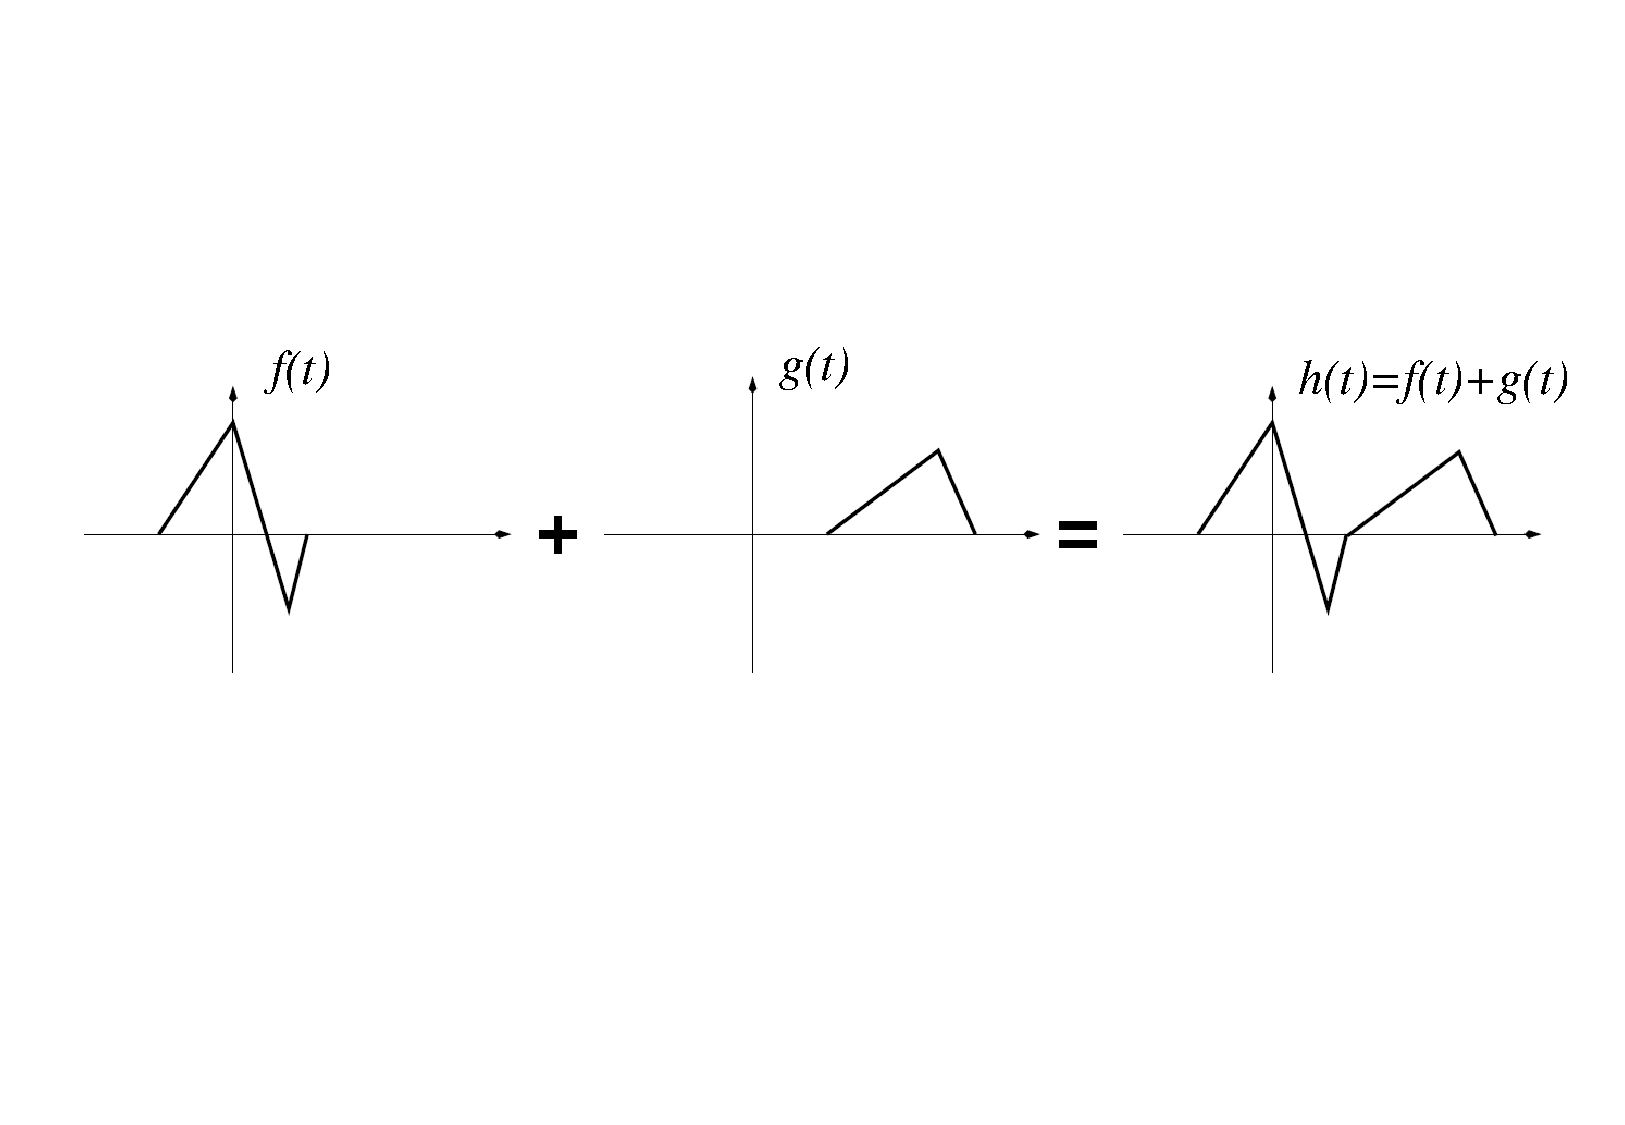
\includegraphics[width=1\textwidth]{img/op_somma_1.pdf}
		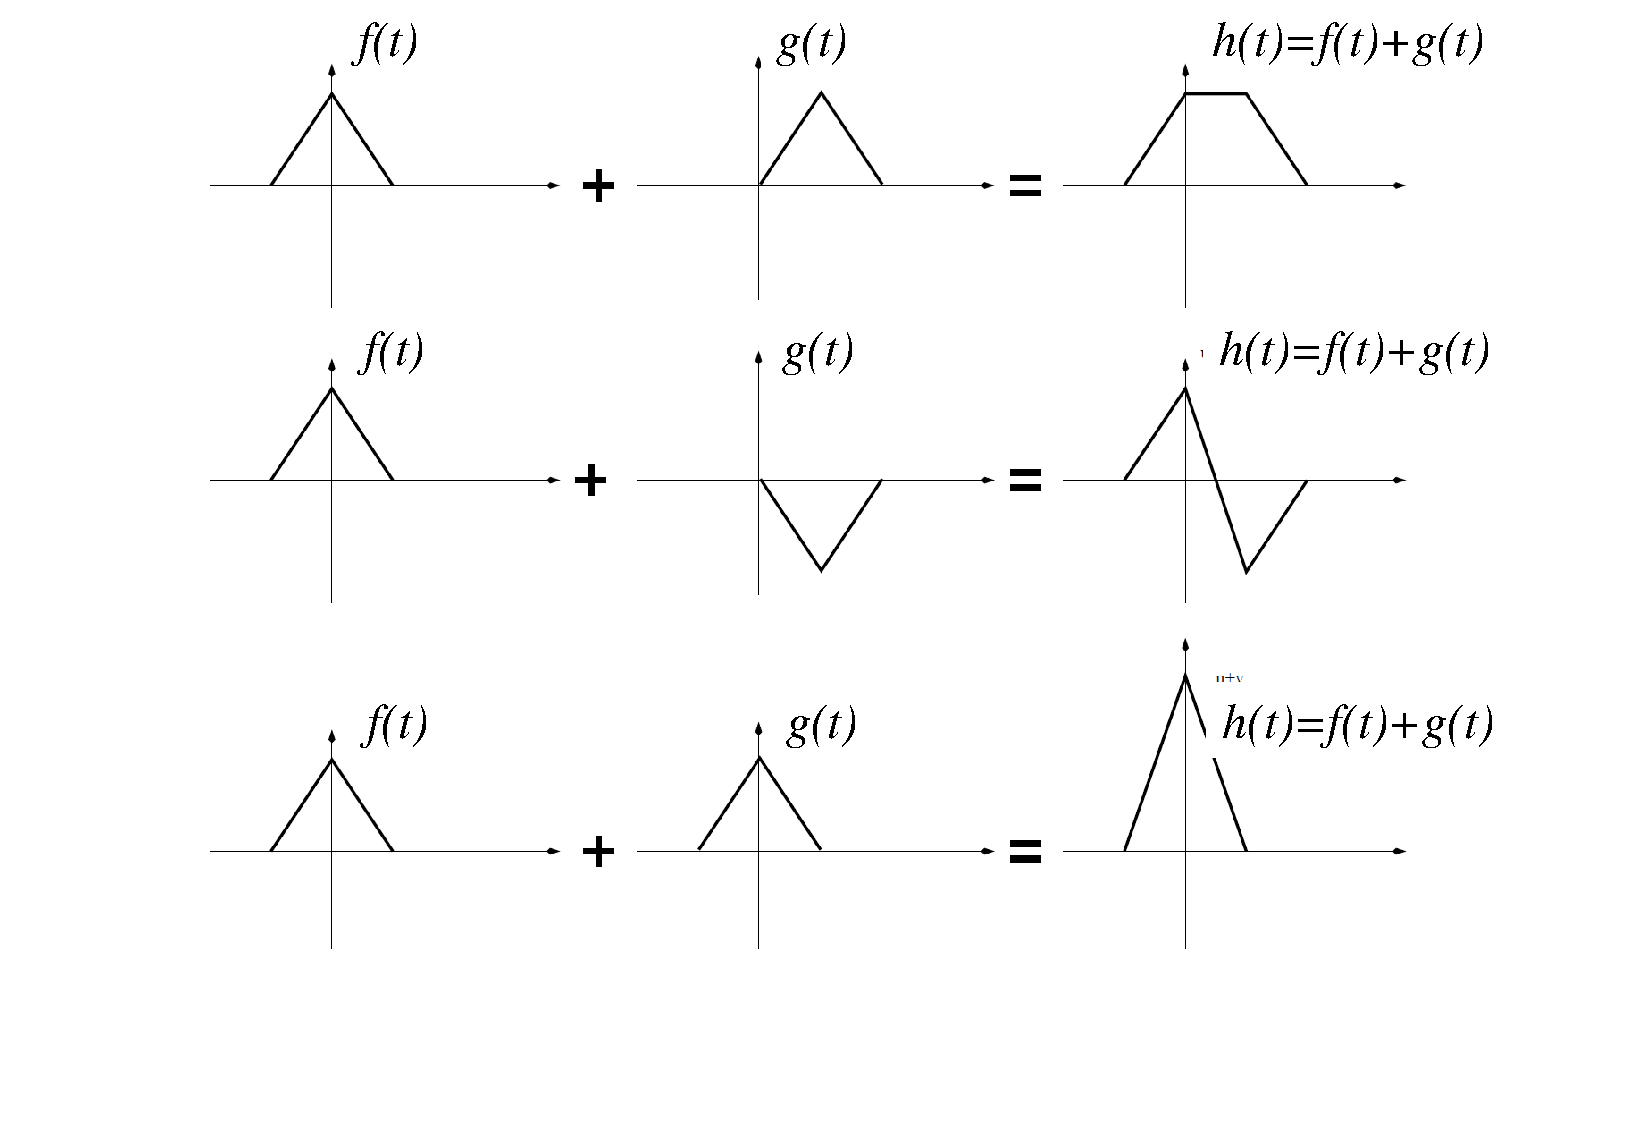
\includegraphics[width=1\textwidth]{img/op_somma_2.pdf}
	\end{figure}

	\newpage
	
	\subsubsection{Shift (o traslazione)}
	
	Lo \textbf{\emph{shift}} (o traslazione) è il cambio di posizione di un segnale. Può essere effettuato:
	
	\begin{itemize}
		\item \textbf{Traslazione a destra} con la funzione $f(t-\tau)$
		\item \textbf{Traslazione a sinistra} con la funzione $f(t+\tau)$
	\end{itemize}
	
	\begin{figure}[!htp]
		\centering
		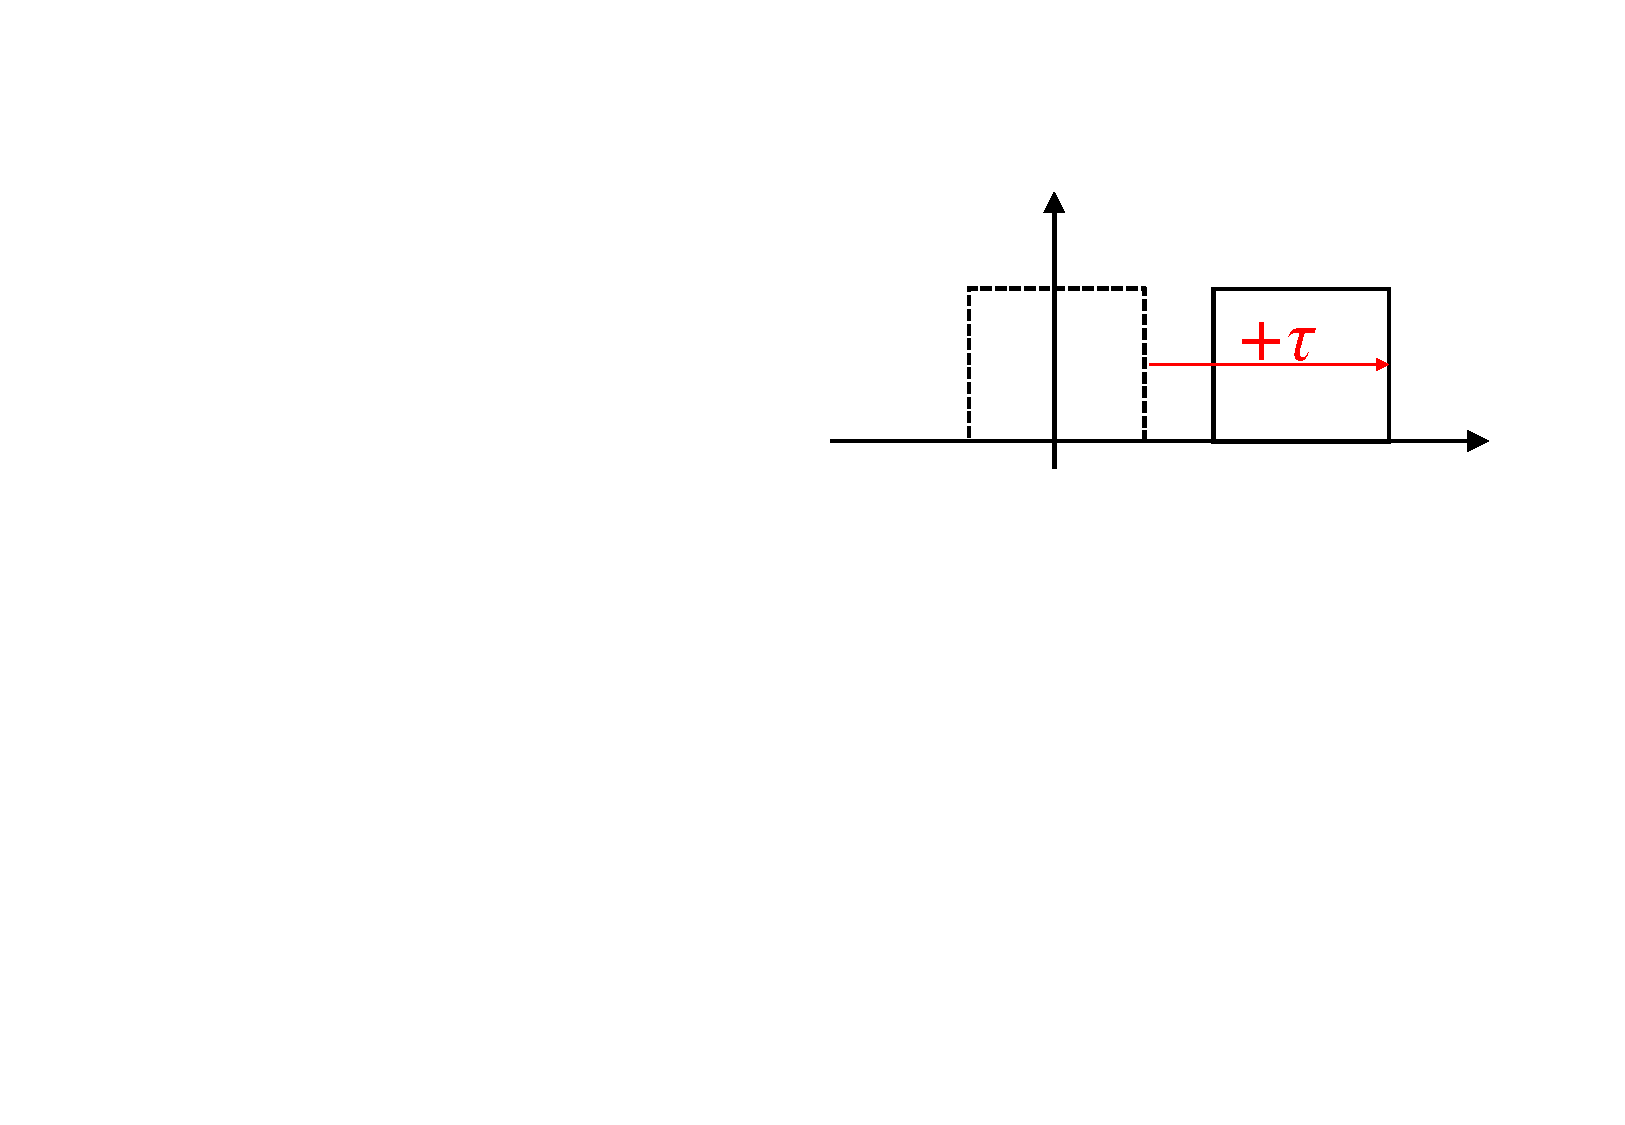
\includegraphics[width=0.5\textwidth]{img/op_shift_dx.pdf}\label{op_shift_dx}
		\caption{Shift a destra}
		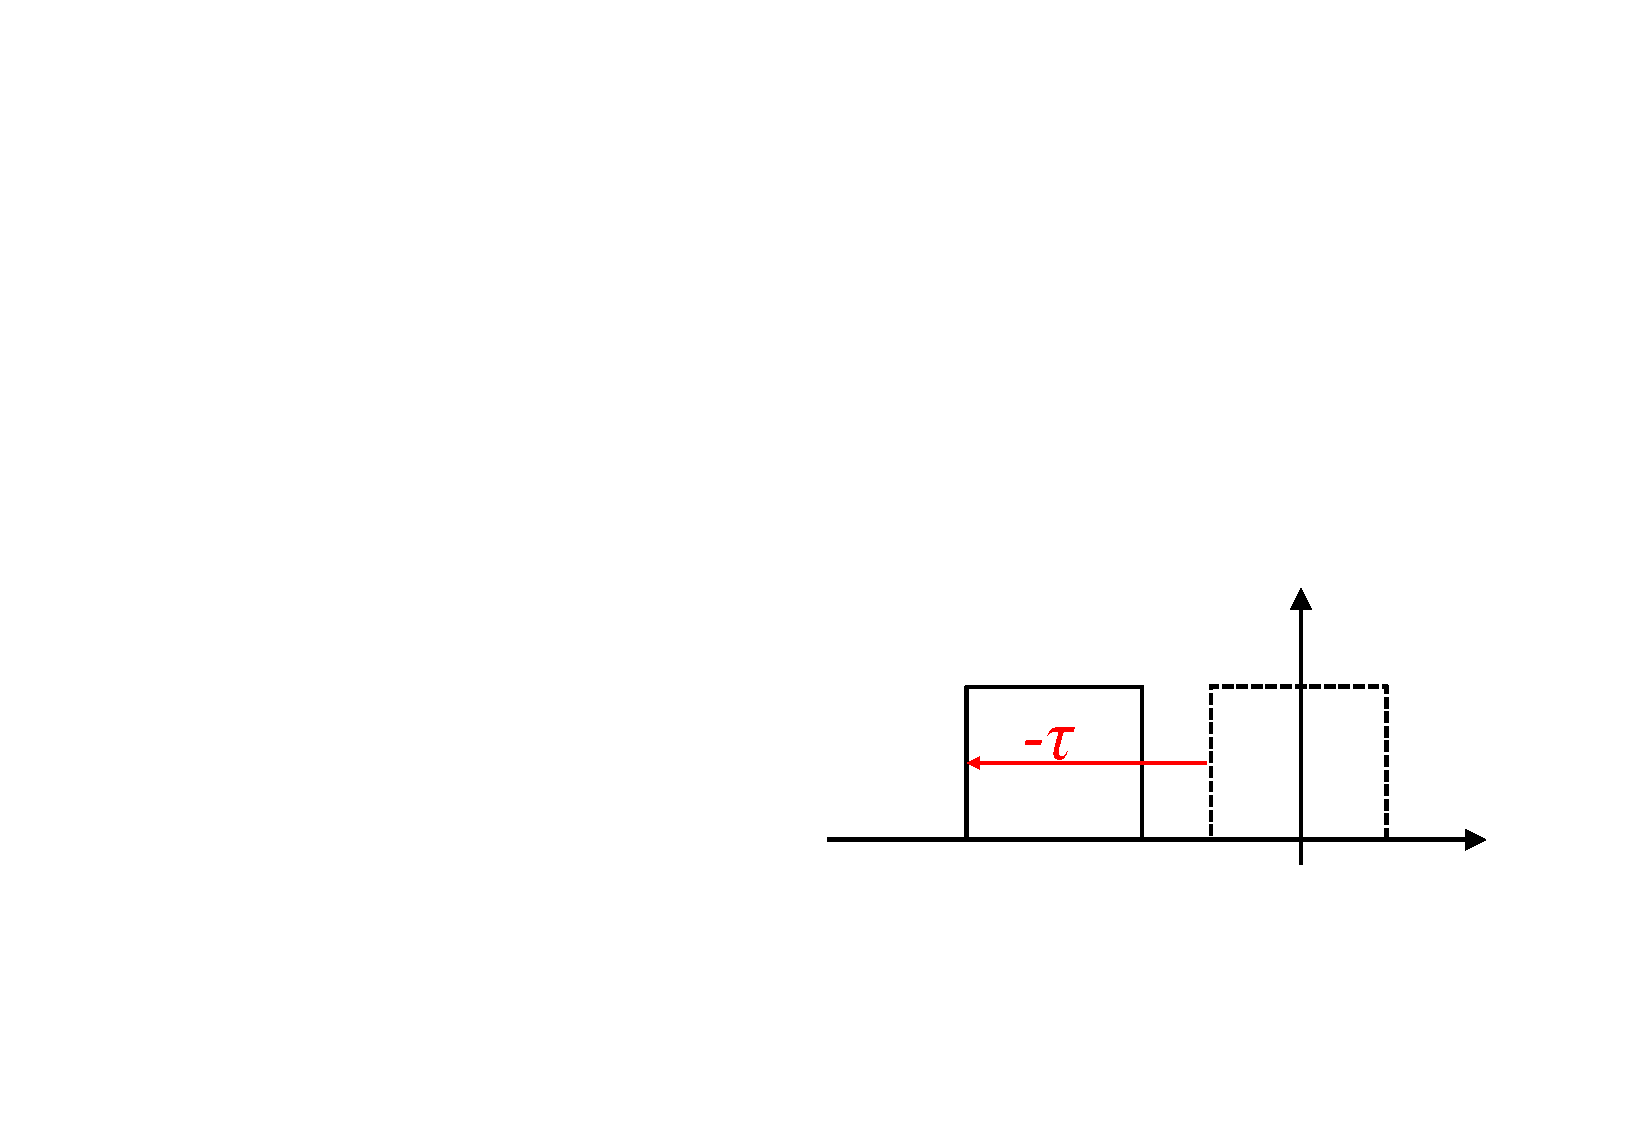
\includegraphics[width=0.5\textwidth]{img/op_shift_sx.pdf}\label{op_shift_sx}
		\caption{Shift a sinistra}
	\end{figure}

	\newpage
	
	\subsubsection{Funzione box $\Pi$ e impulso di Dirac}\label{funzione box e impulso di Dirac}
	
	La funzione \textbf{\emph{box}} è definita nel seguente modo:
	
	\begin{equation*}
		A \Pi\left(\dfrac{x}{b}\right) \hspace{2em} x\in\left[-\dfrac{b}{2}, \dfrac{b}{2}\right]
	\end{equation*}

	\begin{figure}[!htp]
		\centering
		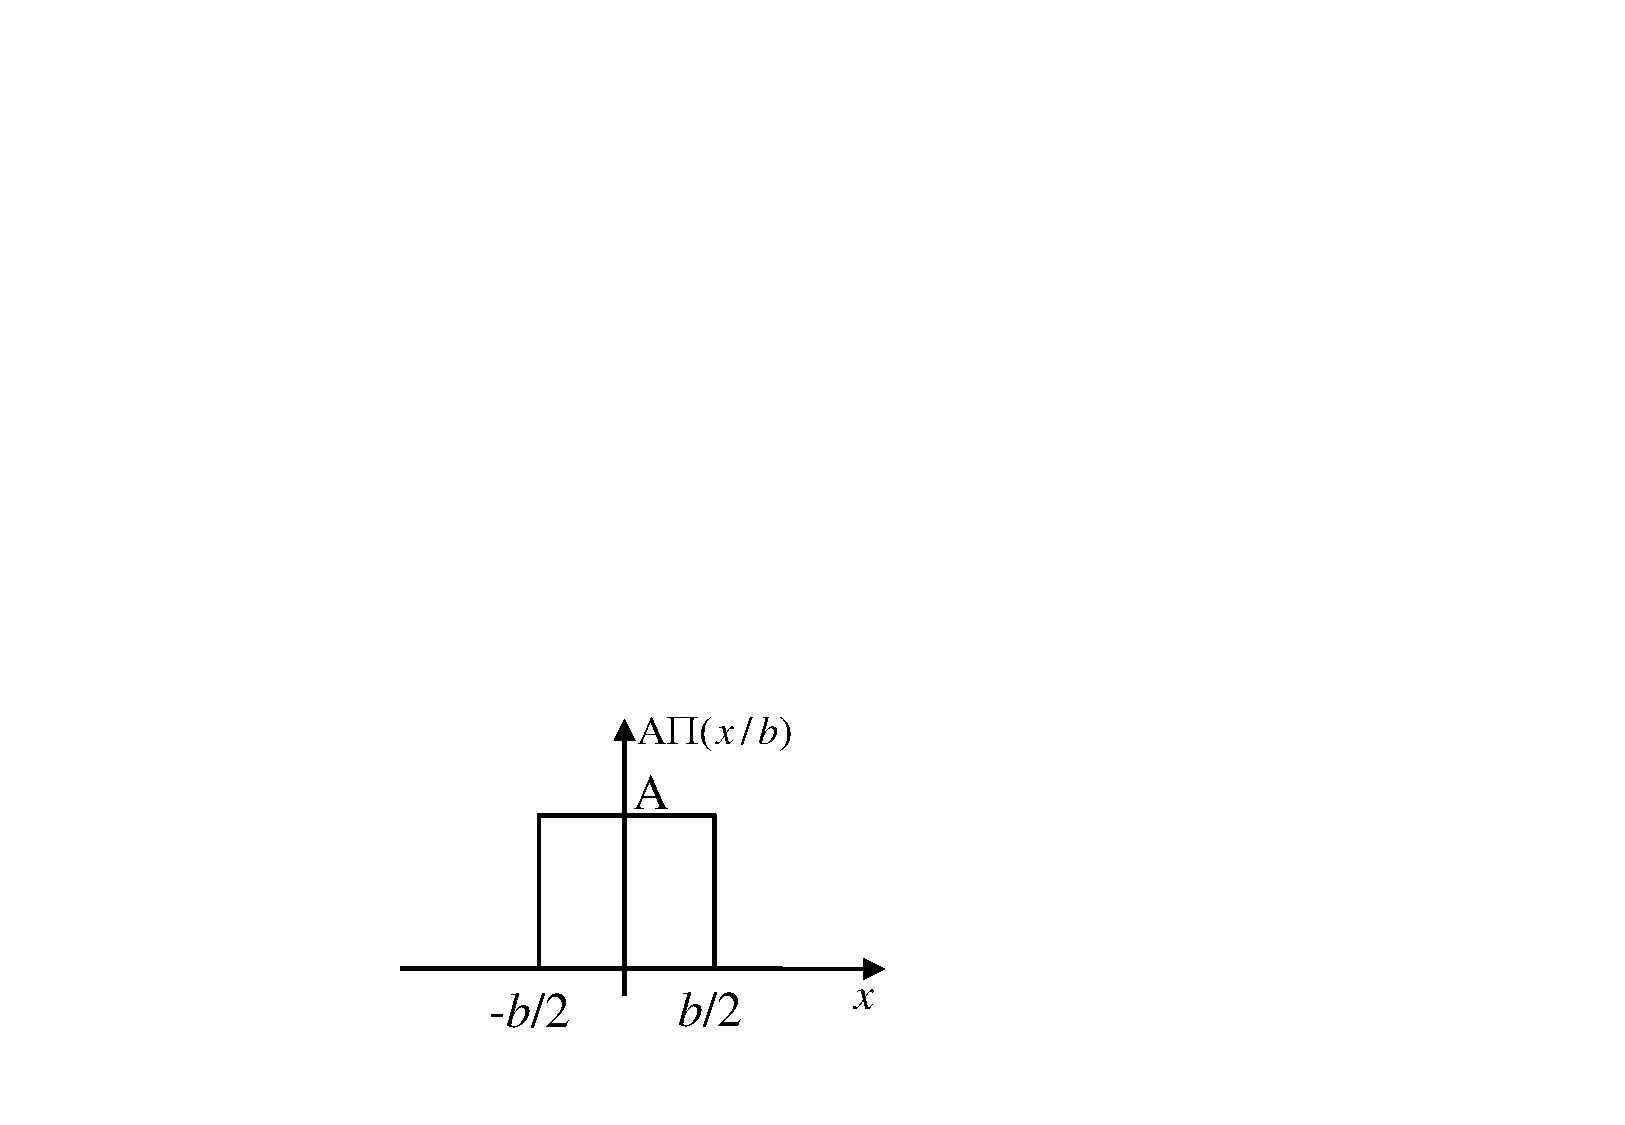
\includegraphics[width=0.4\textwidth]{img/box.pdf}\label{box}
		\caption{Box generica}
	\end{figure}

	La funzione $\delta(x)$ è chiamata \textbf{\emph{impulso unitario}} o \textbf{\emph{impulso di Dirac}} perché è definita nel seguente modo:
	
	\begin{equation*}
		\delta(x) = 
		\begin{cases}
			\infty  & \text{se } x=0 \\
			0		& \text{se } x\ne 0
		\end{cases}
		\hspace{2em} \int_{-\infty}^{\infty} \delta(x)\: dx = 1
	\end{equation*}

	\noindent
	Quindi è un impulso che tende all'infinito solamente quando la $x$ è nell'origine, ma il suo integrale è uguale a $1$. Alcune \textbf{proprietà} dell'impulso:
	
	\begin{enumerate}
		\item $\delta(x-x_0) = 0 \hspace{1em} \forall x\ne x_0$
		\item Data una funzione generica $f$ (\textbf{setacciamento}\label{setacciamento}): $\displaystyle \int_{-\infty}^{\infty} f(x)\delta(x-x_0)\: dt = f(x_0)$
		\item $\delta(x - x_0) = \delta(x_0 - x)$
		\item $\delta(ax) = \dfrac{1}{|a|} \delta(x) \hspace{1em} \forall x \in \mathbb{R} \text{, fissato } a \in \mathbb{R}-\{0\}$
	\end{enumerate}

	\newpage
	
	\subsubsection{Funzione sinc}\label{funzione sinc}
	
	La funzione \textbf{\emph{sinc}} è definita nel seguente modo:
	
	\begin{equation*}
		\mathrm{sinc}(t) = \dfrac{\sin{\left(\pi t\right)}}{\pi t}
	\end{equation*}

	\noindent
	Ha due \textbf{caratteristiche} importanti: (1) l'intersezione con l'asse delle $x$ avviene sempre nei numeri interi positivi e negativi (quindi $1$ e $-1$, $2$ e $-2$, ecc.); (2) il limite $\displaystyle \lim_{t\rightarrow \pm\infty}\mathrm{sinc}(t) = 0$.\newline
	Questa funzione è \textbf{importante per l'analisi nel dominio del tempo} (o \textbf{frequenza}).
	
	\subsubsection{Funzione triangolo $\Lambda$}
	
	La funzione \textbf{\emph{triangolo}} è definita nel seguente modo:
	
	\begin{equation*}
		\Lambda(x) =
		\begin{cases}
			1-|x|, 	& |x| < 1 \\
			0		& \text{altrimenti}
		\end{cases}
	\end{equation*}

	\noindent
	Questa funzione è \textbf{importante per l'analisi spettrale e} per le \textbf{operazioni di convoluzione}.
	
	\subsubsection{Funzione segno ($sgn$)}
	
	La funzione \textbf{\emph{segno}} è definita nel seguente modo:
	
	\begin{equation*}
		\mathrm{sgn}(x) =
		\begin{cases}
			-1, 	& x < 0 \\
			+1,		& x > 0 \\
			0		& x = 0
		\end{cases}
	\end{equation*}
	
	\noindent
	Questa funzione ribalta segnali sopra o sotto l'asse delle $x$.
	
	\subsubsection{Funzione gradino}
	
	La funzione \textbf{\emph{gradino}} è definita nel seguente modo:
	
	\begin{equation*}
		u(x) =
		\begin{cases}
			0 & x < 0 \\
			1 & x \ge 0
		\end{cases}
	\end{equation*}
	
	\noindent
	Questa funzione rappresenta un \textbf{segnale} che si attiva a partire dal tempo specificato e rimane attivo indefinitamente. Attenzione! Non si confonda questo segnale con il segno.
	
	\newpage
	
	\subsubsection{Treno di impulsi}
	
	Il \textbf{\emph{treno di impulsi}} $S_{\Delta T}(x)$ è la somma di un numero infinito di impulsi periodici discreti distanziati di una quantità $\Delta T$:
	
	\begin{equation*}
		S_{\Delta T}(x) = \sum_{n = -\infty}^{\infty} \delta (x - n \Delta T) \hspace{1em} n \in \mathbb{Z}
	\end{equation*}

	\begin{figure}[!htp]
		\centering
		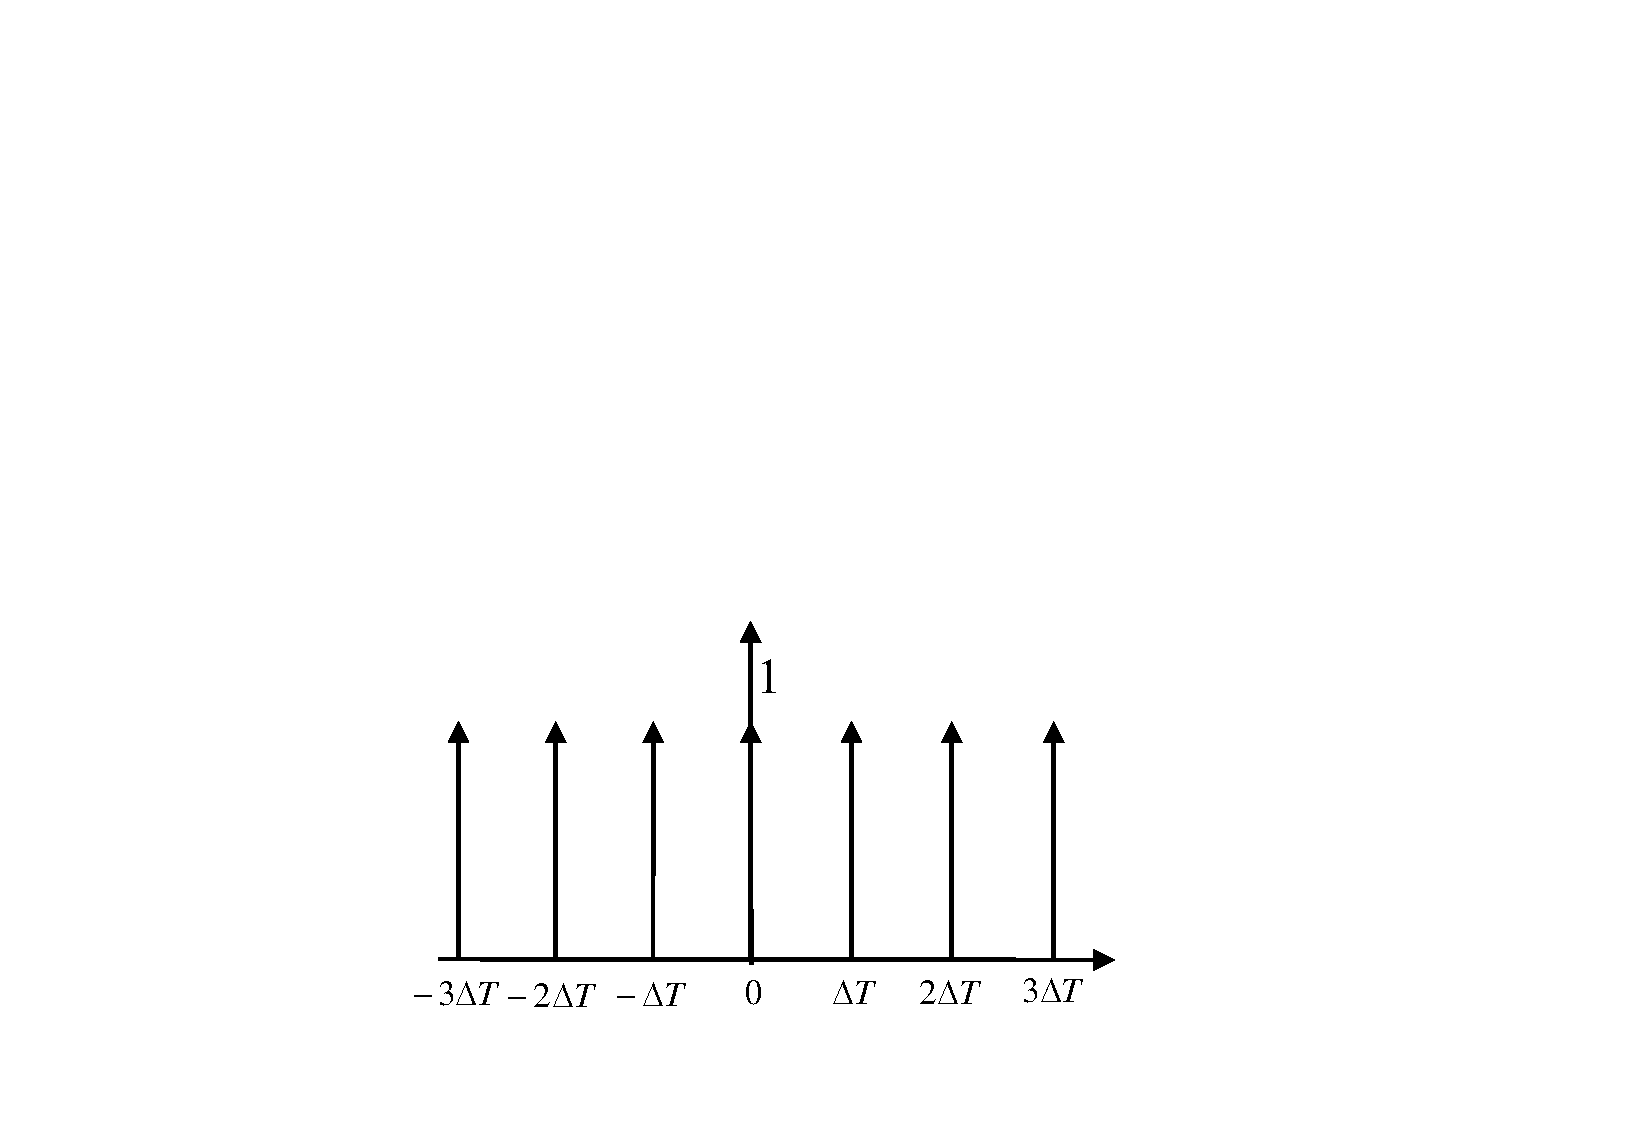
\includegraphics[width=0.5\textwidth]{img/treno_di_impulsi.pdf}\label{treno_di_impulsi}
		\caption{Treno di impulsi}
	\end{figure}

	\subsubsection{Energia di un segnale}
	
	L'\textbf{\emph{energia di un segnale}} è definita nel seguente modo:
	
	\begin{equation*}
		E_f =
		\begin{cases}
			\displaystyle \int_{-\infty}^{+\infty} f^{2}(t)\: dt & \text{se } f \in \mathbb{R} \\
			\displaystyle \int_{-\infty}^{+\infty} \left| f(t) \right|^{2} dt \hspace{1em} \text{con } \left| f(t) \right|^{2} = \tilde{f}(t) f(t), & f \in \mathbb{C}
		\end{cases}
	\end{equation*}
	
	\noindent
	Un segnale si dice \textbf{ad energia finita} (o \textbf{di energia}) se l'integrale che rappresenta l'energia converge ed è diverso da $0$. Quindi:
	
	\begin{itemize}
		\item[\ding{43}] \textbf{Condizione \emph{sufficiente}} all'esistenza della sua trasformata di Fourier. Le funzioni trigonometriche non sono di energia ma hanno comunque la Trasformata di Fourier.
		\item[\ding{42}] \textbf{Condizione \emph{necessaria}} per essere un segnale ad energia finita, all'infinito ($+\infty$ e $-\infty$) l'\textbf{ampiezza} va a zero.
	\end{itemize}

	\noindent
	Alcuni esempi:

	\begin{itemize}
		\item[\ding{80}] \textbf{Segnali di energia.} Impulsi rettangolari, oscillazioni smorzate ($\mathrm{sinc}$);
		\item[\ding{80}] \textbf{Segnali \underline{non} di energia.} Funzioni trigonometriche $\sin$ e $\cos$.
	\end{itemize}

	\noindent
	L'\textbf{unità di misura} è il \emph{joule}.
	
	\subsubsection{Potenza media di un segnale}
	
	La \textbf{\emph{potenza media di un segnale}} è definita nel seguente modo:
	
	\begin{equation*}
		P_f =
		\begin{cases}
			\displaystyle \lim_{T \rightarrow +\infty} \dfrac{1}{T} \int_{-\dfrac{T}{2}}^{+\dfrac{T}{2}} f^{2}(t)\: dt & \text{se } f \in \mathbb{R} \\
			\displaystyle \lim_{T \rightarrow +\infty} \dfrac{1}{T} \int_{-\dfrac{T}{2}}^{+\dfrac{T}{2}} \left|f(t)\right|^{2}\: dt \hspace{1em} \text{con } \left| f(t) \right|^{2} = \tilde{f}(t) f(t), & f \in \mathbb{C}
		\end{cases}
	\end{equation*}
	
	\noindent
	Un segnale si dice \textbf{a potenza finita} (o \textbf{di potenza}) se l'integrale che rappresenta la potenza converge ed è diverso da $0$. L'\textbf{unità di misura} è il \emph{watt}.\newline
	Infine, un segnale ad energia finita ha la potenza che tende a zero (per cui un segnale non può appartenere ad entrambe le categorie). Invece, esistono segnali che non sono né di energia, n* di potenza finita.
	
	\newpage
	
	\subsection{Altre operazioni fondamentali}
	
	\subsubsection{Rescaling (o riscalatura)}
	
	La funzione di \textbf{\emph{rescaling}} è definita nel seguente modo:
	
	\begin{equation*}
		\forall f(t) : D_1 \in \mathbb{R}, \hspace{1em} \omega \ne 0
	\end{equation*}
	
	\noindent
	Simile allo \emph{shift}, il \emph{rescaling} ha una definizione generica e due varianti:
	
	\begin{itemize}
		\item \textbf{Definizione generica} con la funzione semplice $f(t)$ (immagine~\ref{rescaling}).
		\item \textbf{Ritardo \underline{lineare} del segnale di un fattore $\omega$} con la funzione $f(\omega t), 0 < \omega < 1$ (immagine~\ref{rescaling_ritardo}).
		\item \textbf{Accelero \underline{lineare} del segnale di un fattore $\omega$} con la funzione $f(\omega t), \omega > 1$ (immagine~\ref{rescaling_accelero}).
	\end{itemize}
	
	\begin{figure}[!htp]
		\centering
		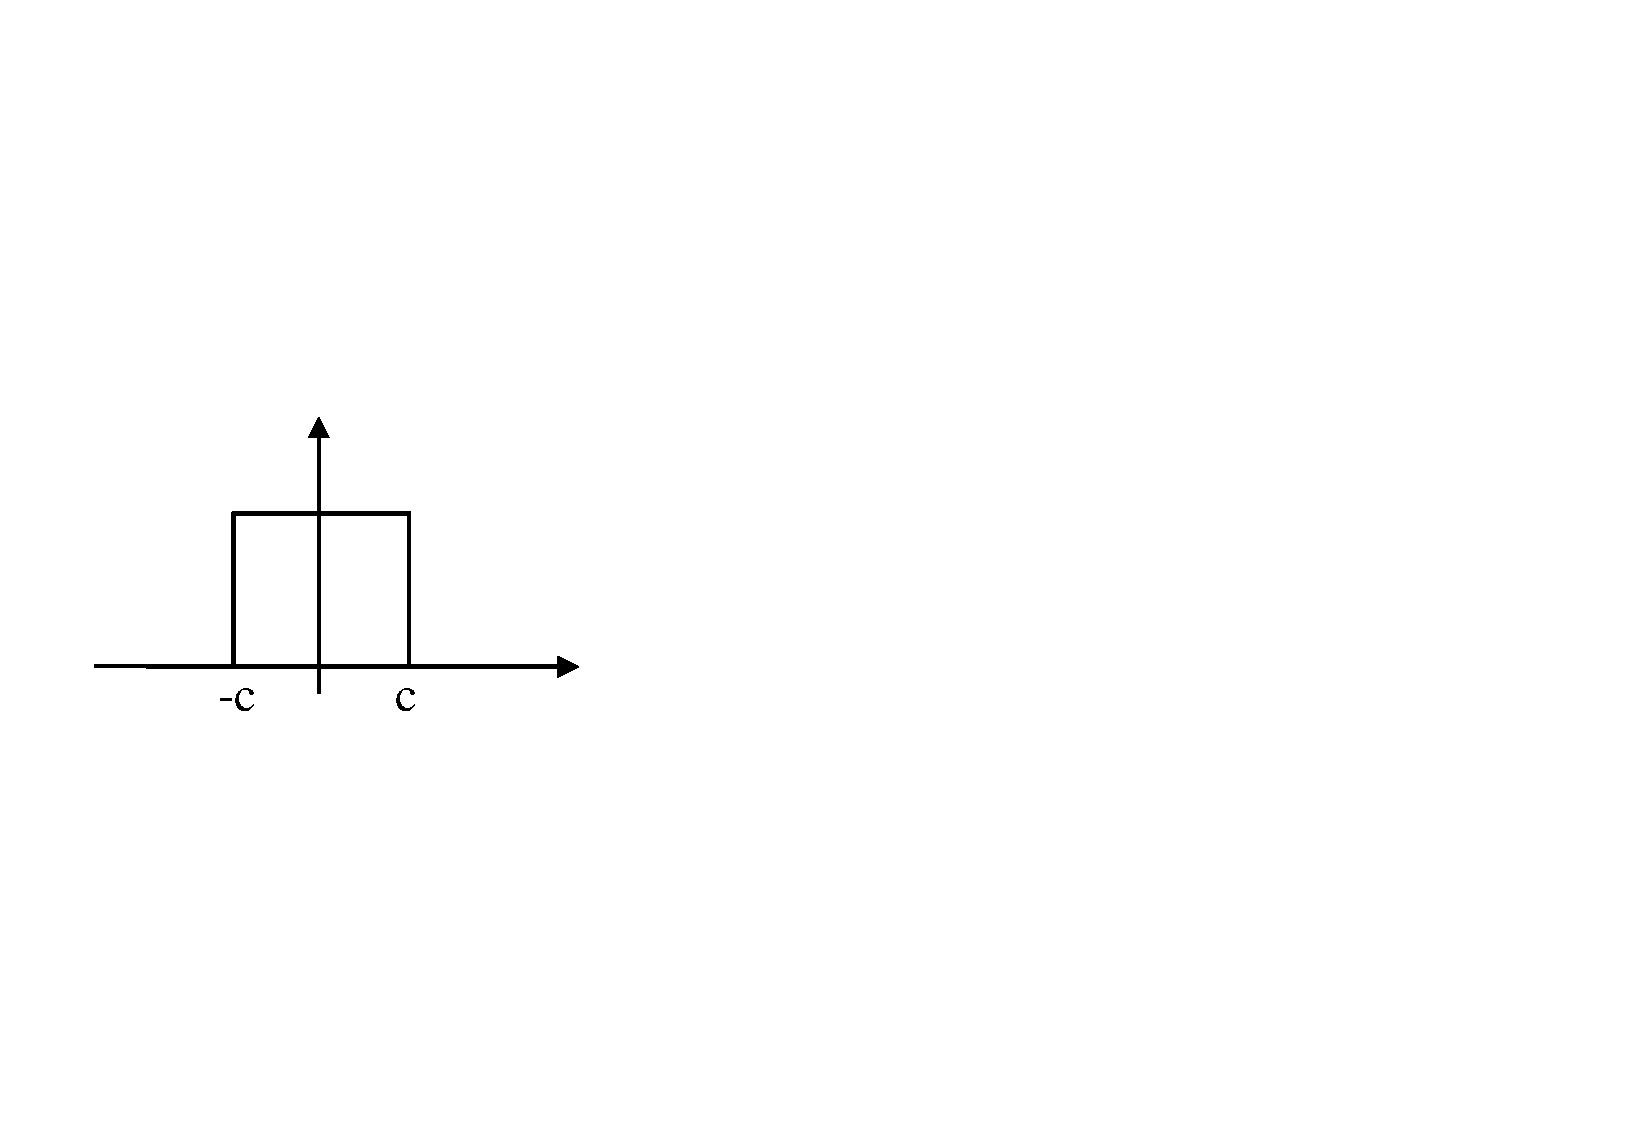
\includegraphics[width=0.5\textwidth]{img/rescaling.pdf}
		\caption{Definizione generica}\label{rescaling}
		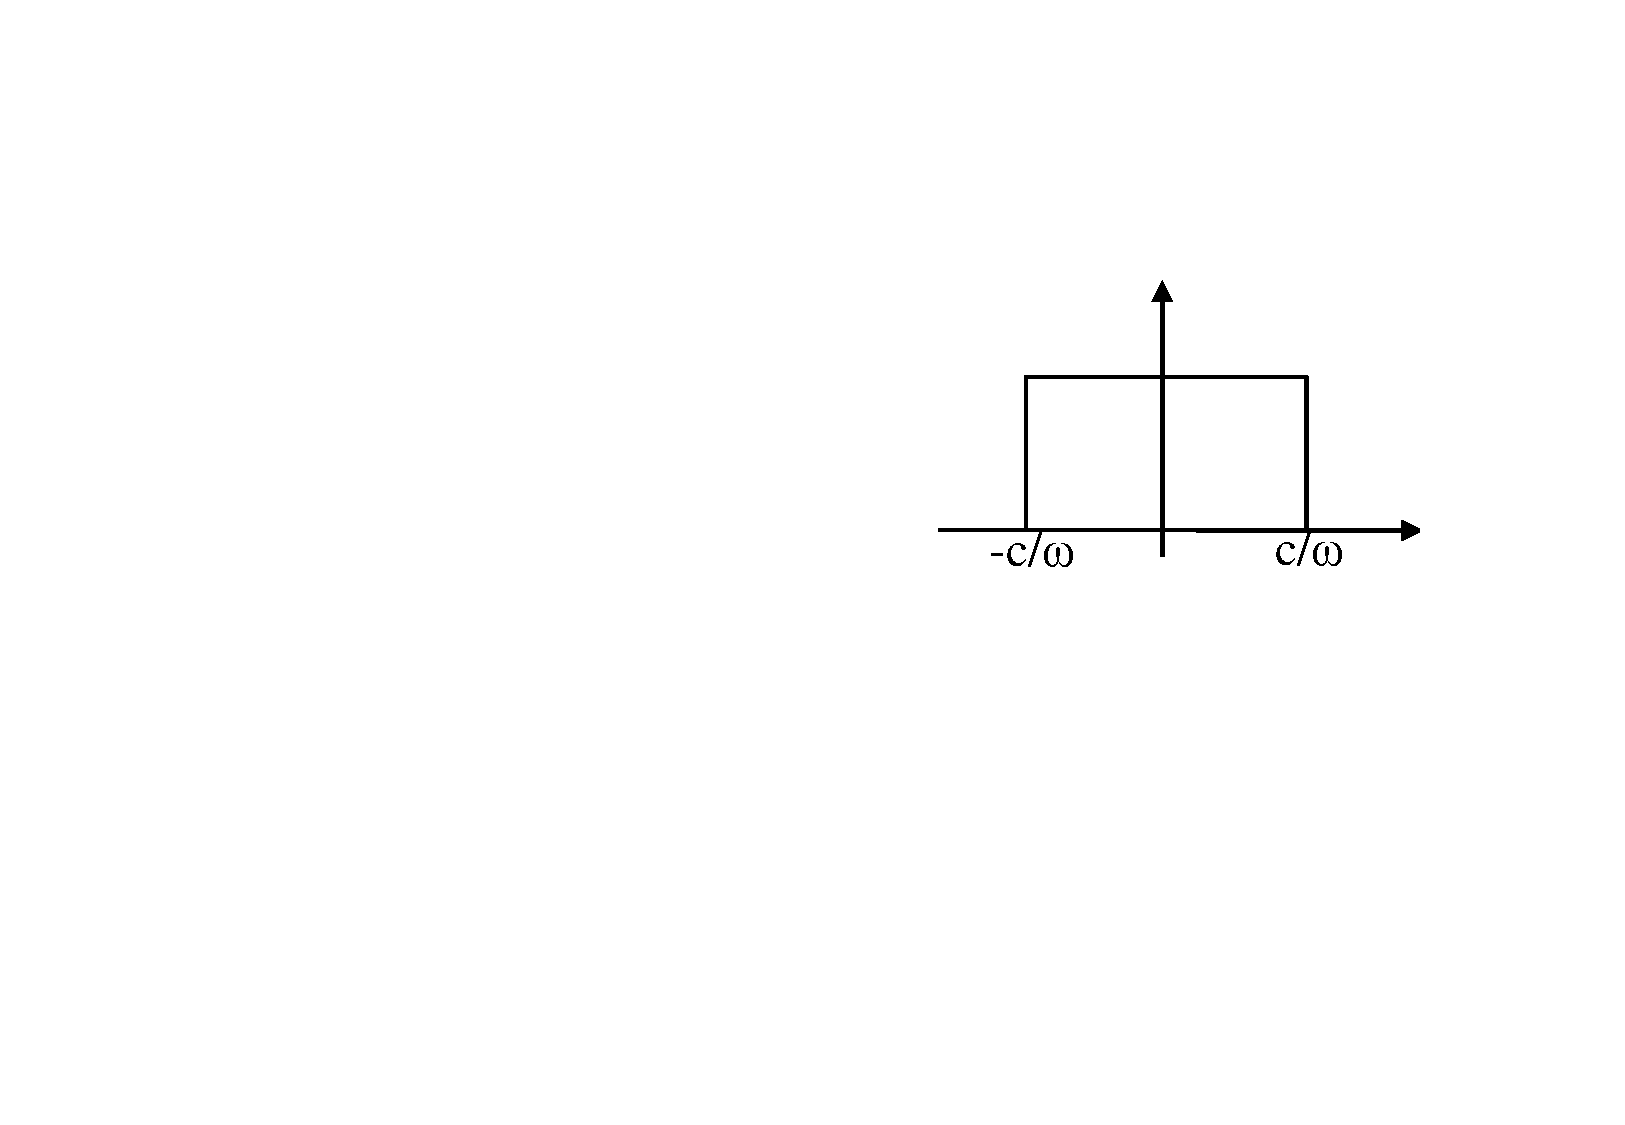
\includegraphics[width=0.5\textwidth]{img/rescaling_ritardo.pdf}
		\caption{Ritardo \underline{lineare} del segnale di un fattore $\omega$}\label{rescaling_ritardo}
		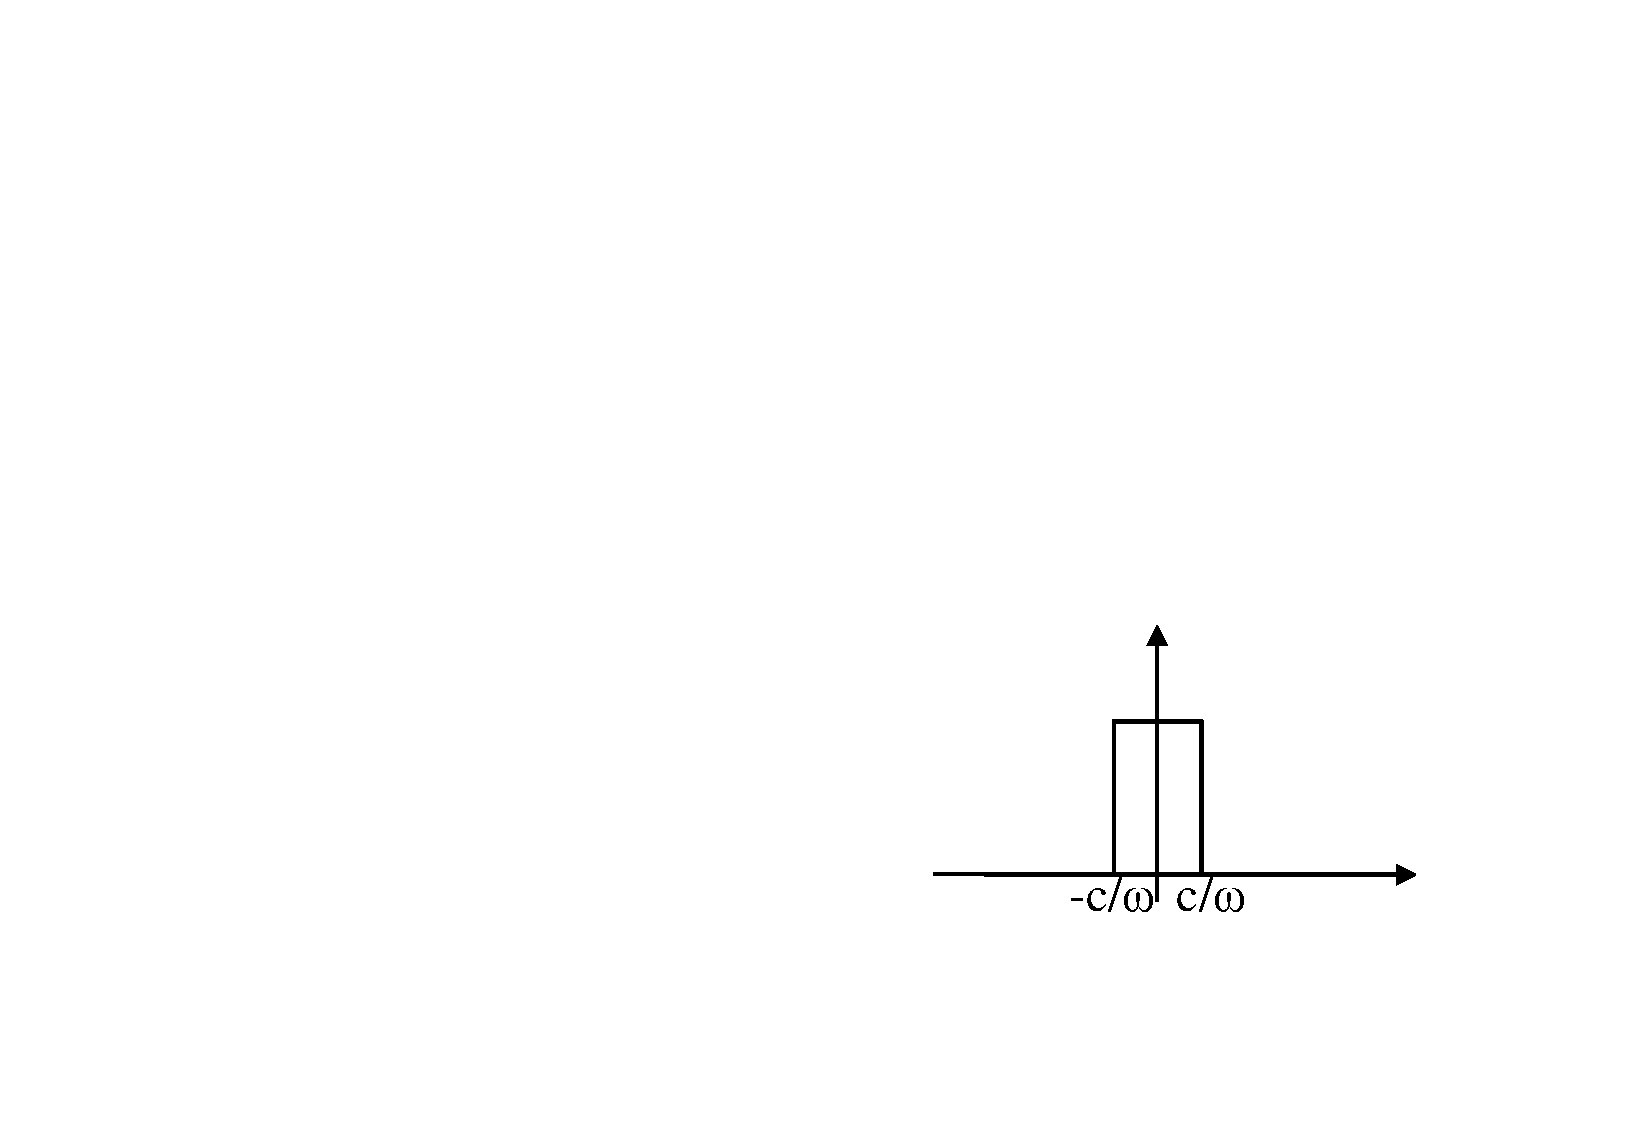
\includegraphics[width=0.5\textwidth]{img/rescaling_accelero.pdf}
		\caption{Accelero \underline{lineare} del segnale di un fattore $\omega$}\label{rescaling_accelero}
	\end{figure}

	\subsubsection{Cross-Correlazione}\label{cross correlazione}
	
	Dati $f_1(\tau), f_2(\tau)$ segnali continui, $\tau\in\mathbb{R}$ il segnale di \textbf{\emph{cross-correlazione}} viene definito come:
	
	\begin{equation*}
		\displaystyle f_1 \otimes f_2 (t) = \int_{-\infty}^{+\infty} \tilde{f_1}(\tau) f_2(\tau - t)\: d\tau
	\end{equation*}

	\noindent
	In cui $\tilde{f_1}(\tau)$ rappresenta un \emph{complesso coniugato}. Nel caso in cui $f_1$ è reale, allora $\tilde{f_1}(\tau) \rightarrow f_1(\tau)$. \newline
	Infine, con $t = 0$ si ha l'\textbf{\emph{integrale di cross-correlazione}}, il quale è definito se l'integrale converge (ovviamente se il segnale non è né di energia, né di potenza, la convergenza non esiste!).
	
	\newpage
	
	
	
	
	\subsubsection{Esercizi d'esame}
	
	\textcolor{Red3}{\textbf{\emph{Esercizio.}}}
	
	Il primo esercizio fornisce una funzione $f(t)$:
	
	\begin{equation*}
		f(t) = \Pi \left(\dfrac{t-2}{4}\right) e^{-2t}
	\end{equation*}

	\noindent
	Le \textbf{richieste} dell'esercizio sono le seguenti:
	
	\begin{enumerate}[label=\Roman*]
		\item Rappresentare graficamente il segnale;
		
		\item Calcolare sia l'energia che la potenza media. Inoltre, dire se $f(t)$ è una funzione di energia o di potenza fornendo una motivazione valida. Infine, calcolare l'energia o la potenza nel caso in cui $f(t)$ sia solo composta da $e^{-2t}$;
		
		\item Scrivere l'espressione analitica rispetto $z(t) = -f(-t)$ e $v(t) = f(t+4)$
	\end{enumerate}

	\noindent
	\textcolor{Green4}{\textbf{\emph{Risoluzione I.}}}
	
	\noindent
	Il \textbf{primo passo} è quello di scomporre la funzione così da avere una visione più chiara sulle operazioni da effettuare:
	
	\begin{equation*}
		f(t) = \Pi \left(\dfrac{t-2}{4}\right) e^{-2t} \longrightarrow f(t) = \Pi \left(\dfrac{1}{4} \cdot \left(t - 2\right)\right)
	\end{equation*}

	\noindent
	Come si può osservare, ci sono due operazioni da eseguire. Quindi, dopo l'esplicitazione si esegue la rappresentazione del segnale base $\Pi(t)$:
	
	\begin{figure}[!htp]
		\centering
		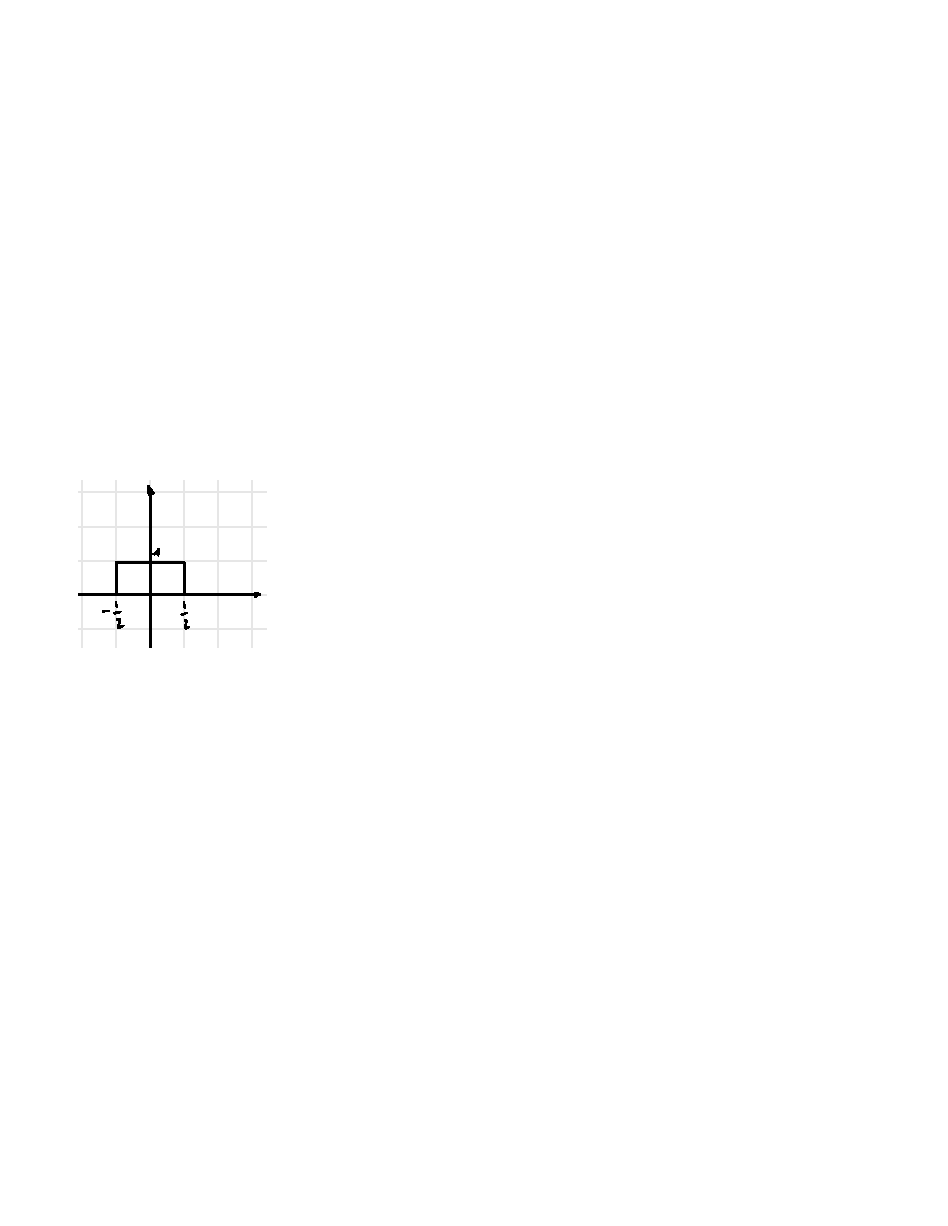
\includegraphics[width=0.4\textwidth]{img/ex_exam/Pi_func_1.pdf}
		\caption{Rappresentazione della funzione $f(t)$, ovvero un box.}
	\end{figure}

	\newpage
	Adesso si esegue l'operazione di moltiplicazione per un fattore che in questo caso è $\dfrac{1}{4}$. Quindi si rappresenta la box $\Pi\left(\dfrac{1}{4}\cdot t\right)$:
	
	\begin{figure}[!htp]
		\centering
		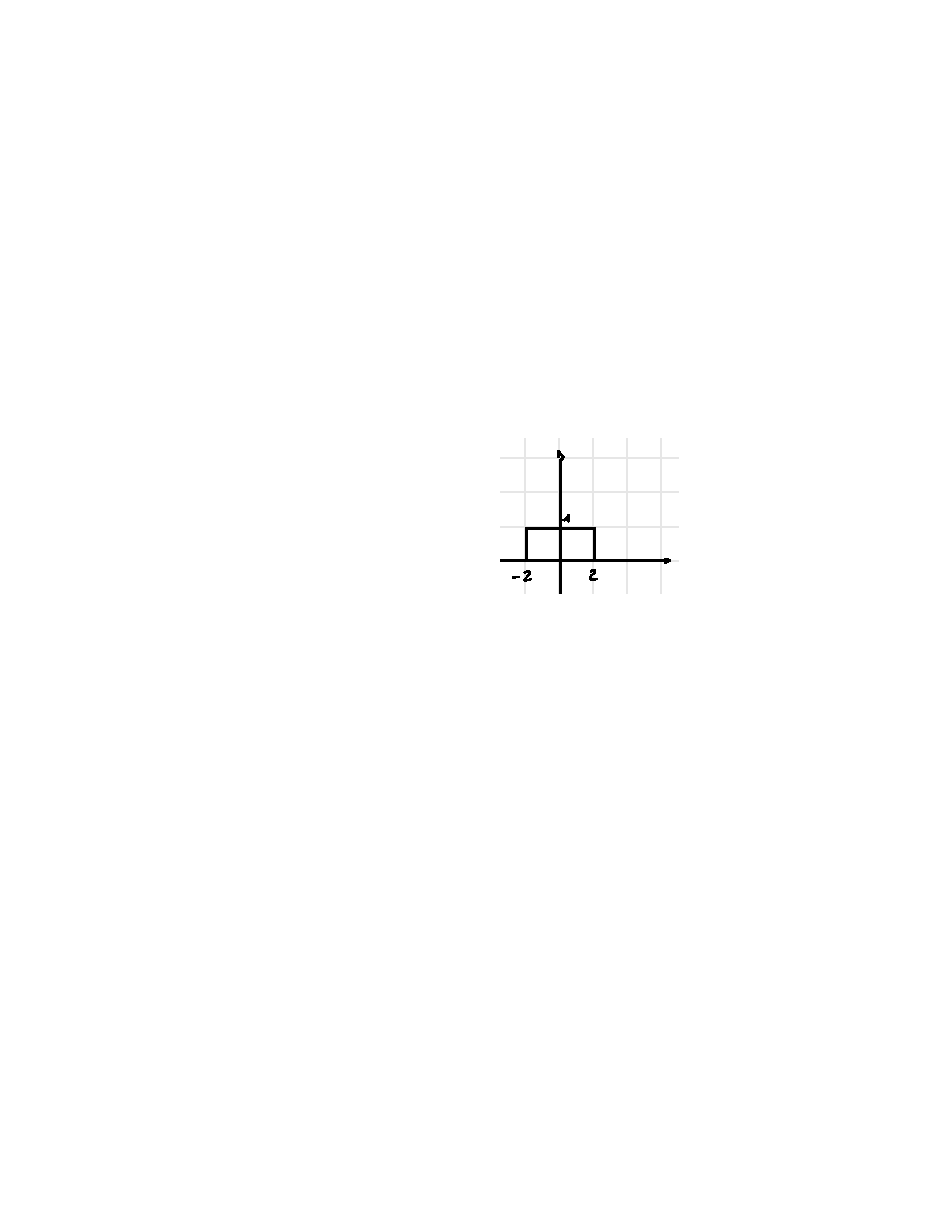
\includegraphics[width=0.4\textwidth]{img/ex_exam/Pi_func_1-Mod.pdf}
		\caption{Box $\Pi\left(\dfrac{1}{4}\cdot t\right)$ allargata.}
	\end{figure}

	\noindent
	L'operazione che è stata effettuata è stata semplicemente considerare la box del tipo $\Pi\left(\dfrac{t}{4}\right)$. Ricordandosi le nozioni del corso di Sistemi, per definizione quindi la box è definita nell'intervallo $-2, +2$.
	
	Infine, viene applicata l'ultima operazione, ovvero il $-2$ all'incognita $t$. Quindi, la funzione box diventerà $\Pi\left(\dfrac{1}{4}\left(t-2\right)\right)$ e la sua rappresentazione grafica sarà uno shift a destra (ritardo):
	
	\begin{figure}[!htp]
		\centering
		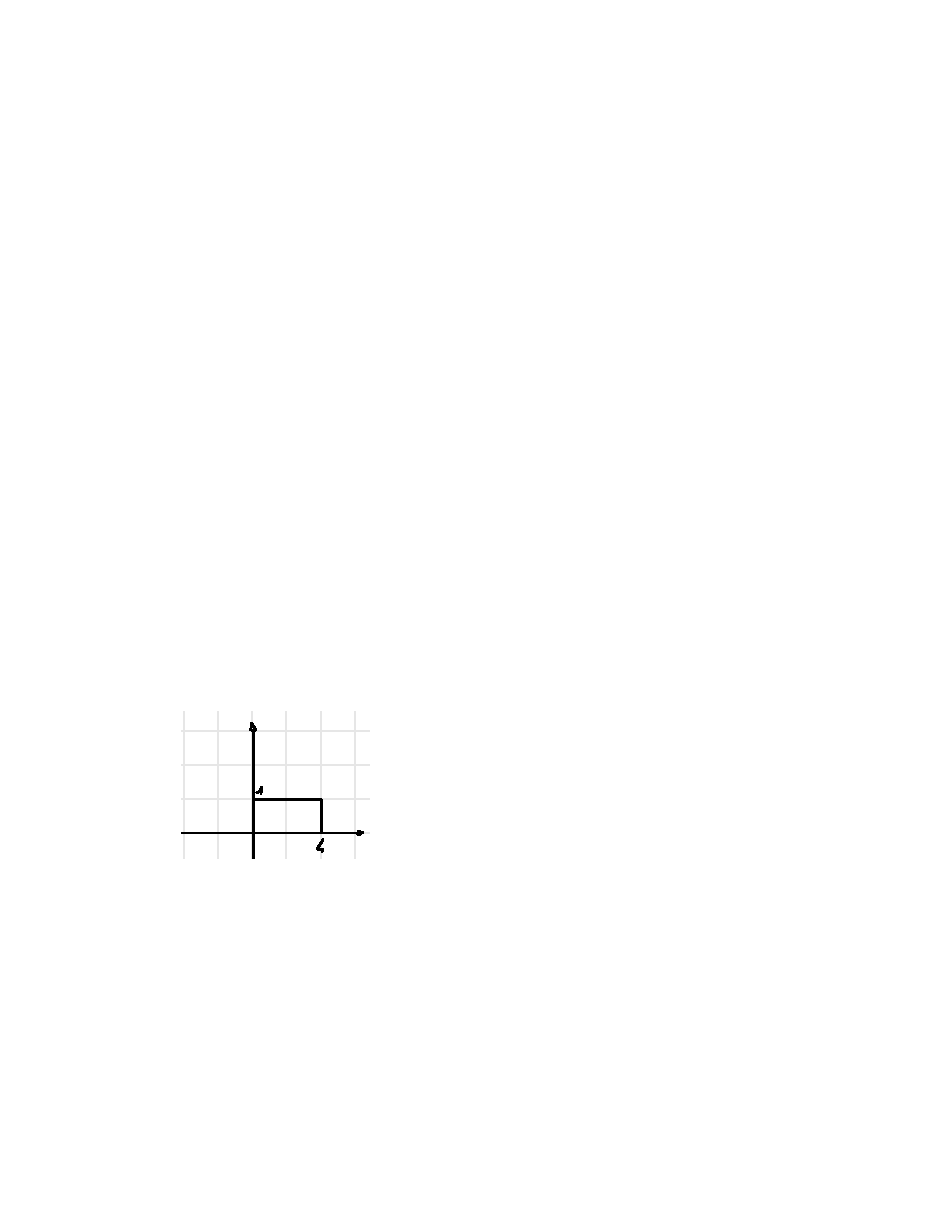
\includegraphics[width=0.4\textwidth]{img/ex_exam/Pi_func_1-Mod2.pdf}
		\caption{Box $\Pi\left(\dfrac{1}{4}\left(t-2\right)\right)$ dopo lo shift a destra.}
	\end{figure}

	\newpage

	Il \textbf{primo punto si conclude} con la rappresentazione del segnale $e^{-2t}$ e la sua combinazione con la box. Quindi:
	
	\begin{figure}[!htp]
		\centering
		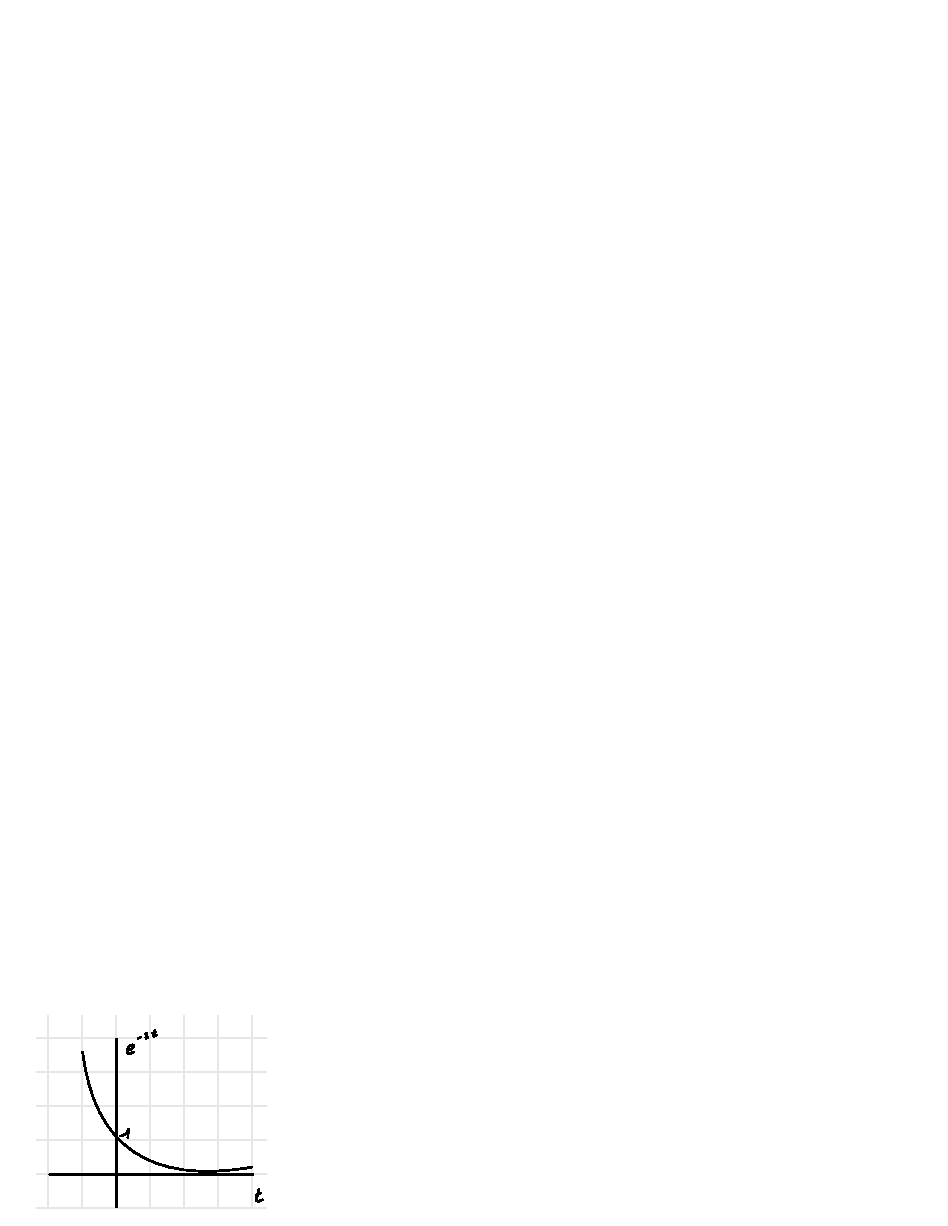
\includegraphics[width=0.4\textwidth]{img/ex_exam/E_func_1.pdf}
		\caption{Rappresentazione della funzione $e^{-2t}$}
	\end{figure}

	\noindent
	E infine la sua concatenazione con la box, quindi una sorta di applicazione di un filtro:
	
	\begin{figure}[!htp]
		\centering
		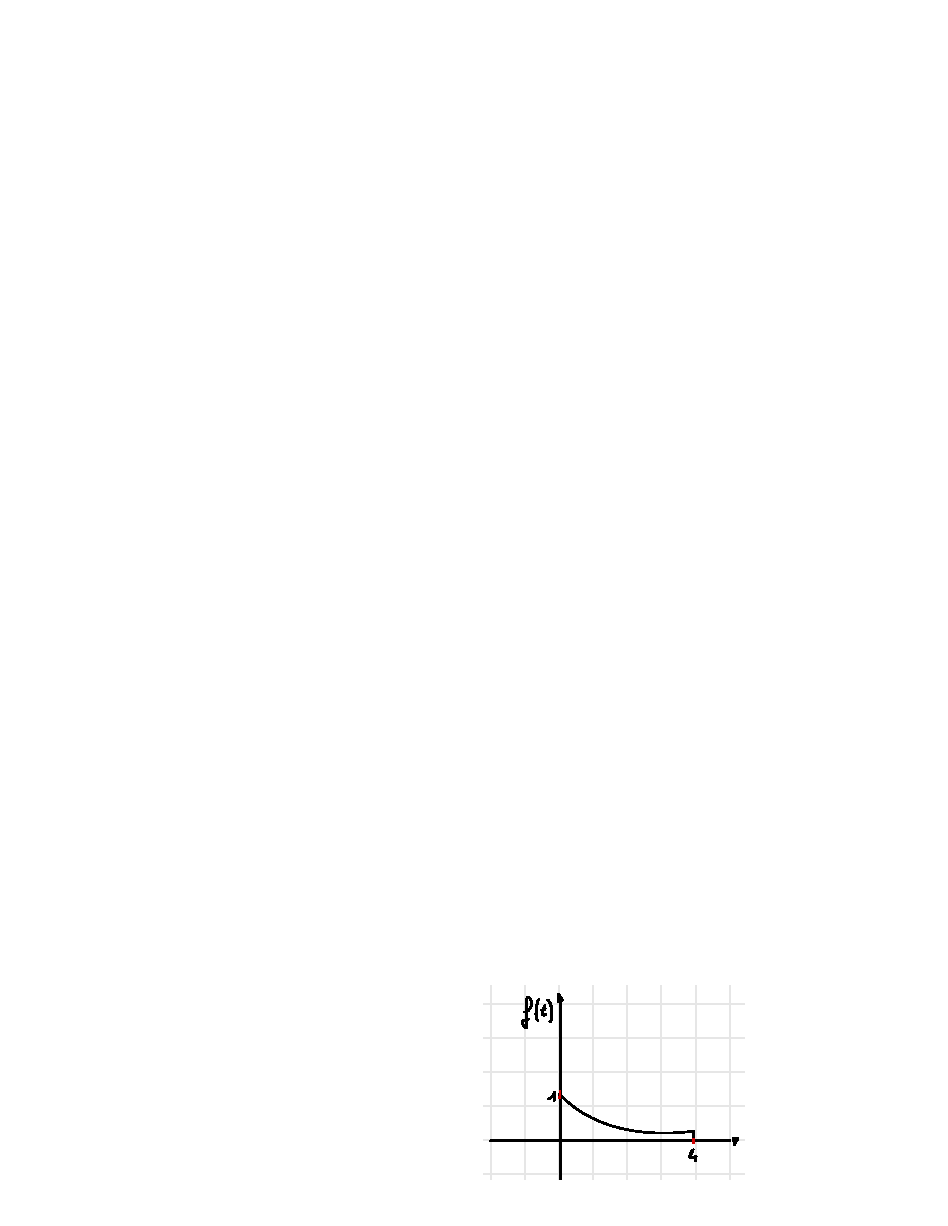
\includegraphics[width=0.4\textwidth]{img/ex_exam/Sol_func_1.pdf}
		\caption{Rappresentazione finale della funzione $f(t) = \Pi \left(\dfrac{t-2}{4}\right) e^{-2t}$}\label{ex1_grafico}
	\end{figure}

	\newpage

	\noindent
	\textcolor{Green4}{\textbf{\emph{Risoluzione II.}}}

	Guardando la figura~\ref{ex1_grafico} si può già intuire che tipo di segnale sia. Infatti, dato che è limitato e non si estende all'infinito, per definizione è un \textbf{segnale finito}, quindi \textbf{di energia} e \underline{non} di potenza. Per dimostrare questa affermazione, si eseguono i calcoli:
	
	\begin{gather*}
		\textbf{Definizione di energia: } E_{f} = \int_{-\infty}^{\infty}{\left|f(t)\right|^2\:\mathrm{d}t} = \int_{-\infty}^{\infty}{f(t)^2\:\mathrm{d}t} \\
		\textbf{Definizione di potenza: } P_{f} = \lim_{T\rightarrow\infty}{\dfrac{1}{T} \int_{-\frac{T}{2}}^{\frac{T}{2}}{f^{2}(t)\:\mathrm{d}t}}
	\end{gather*}

	\noindent
	Dopo le definizioni, si esegue l'effettivo calcolo con i valori numerici:
	
	\begin{gather*}
		\textbf{Energia finita} \\
		E_{f} = \int_{0}^{4}{e^{-4t}\:\mathrm{d}t} = \left.\dfrac{e^{-4t}}{-4}\right\vert_{0}^{4} = \dfrac{-e^{-16}+1}{4} = \dfrac{1}{4} \ne 0 \\
		\textbf{Potenza finita} \\
		P_{f} = \lim_{T\rightarrow\infty}{\dfrac{1}{T} \int_{0}^{4}{e^{-4t}\:\mathrm{d}t}} = \lim_{T\rightarrow\infty}{\dfrac{1}{T}\cdot\dfrac{1}{4}} = 0
	\end{gather*}

	\noindent
	Come si osserva dai risultati, \underline{è} un segnale di energia finita poiché è un valore noto, invece \underline{non è} un segnale di potenza poiché il risultato è zero e non rispetta la definizione.
	
	Al contrario, se la funzione fosse composta solamente dall'esponenziale, il calcolo dell'energia e della potenza sarebbe:
	
	\begin{gather*}
		\textbf{Energia: } E_{f} = \int_{-\infty}^{\infty}{e^{-4t}\:\mathrm{d}t} = \left.\dfrac{e^-4t}{-4}\right\vert_{-\infty}^{\infty} = \lim_{T\rightarrow\infty}{\dfrac{e^{-4t} - e^{4t}}{-4}} = \infty \\
		\textbf{Potenza: } P_{f} = \lim_{T\rightarrow\infty}{\dfrac{1}{T} \int_{-\frac{T}{2}}^{\frac{T}{2}}{e^{-4t}\:\mathrm{d}t}} = \lim_{T\rightarrow\infty}\left.\dfrac{e^{-4t}}{-4}\cdot\dfrac{1}{T}\right\vert_{-\frac{T}{2}}^{\frac{T}{2}} = \lim_{T\rightarrow\infty}\dfrac{e^{-2T} - e^{2T}}{-4T} = \infty
	\end{gather*}

	\noindent
	Come si evince dai calcoli, il segnale non è né di energia né di potenza perché entrambi i risultati sono uguali a infinito.\newline
	
	\noindent
	\textcolor{Green4}{\textbf{\emph{Risoluzione III.}}}
	
	Considerando la funzione $z(t)$, si osserva che è la copia simmetrica rispetto all'origine di $f(t)$. Invece, la funzione $v(t)$ è identica alla funzione $f(t)$ ma ``shiftata'' a sinistra di $4$:
	
	\begin{equation*}
		f(t) = -f(-t) \hspace{2em} v(t) = f(t + 4)
	\end{equation*}

	\newpage
	
	\noindent
	\textcolor{Red3}{\textbf{\emph{Esercizio 2.}}}
	
	\noindent
	Il secondo esercizio fornisce una funzione $f(t)$:
	
	\begin{equation*}
		f(t) = \mathrm{sgn }\left(a\cdot\cos{\left(\dfrac{2\pi}{T_0} t\right)}\right)
	\end{equation*}
	
	\noindent
	Con $T_0 = 2$. Le \textbf{richieste} dell'esercizio sono le seguenti:
	
	\begin{enumerate}[label=\Roman*]
		\item Rappresentare graficamente il segnale;
		
		\item Calcolare sia l'energia che la potenza media. Inoltre, dire se $f(t)$ è una funzione di energia o di potenza fornendo una motivazione valida.
	\end{enumerate}
	
	\noindent
	\textcolor{Green4}{\textbf{\emph{Risoluzione I.}}}
	
	\noindent
	Viene rappresentato il segnale della funzione segno $\mathrm{sng}$:
	
	\begin{figure}[!htp]
		\centering
		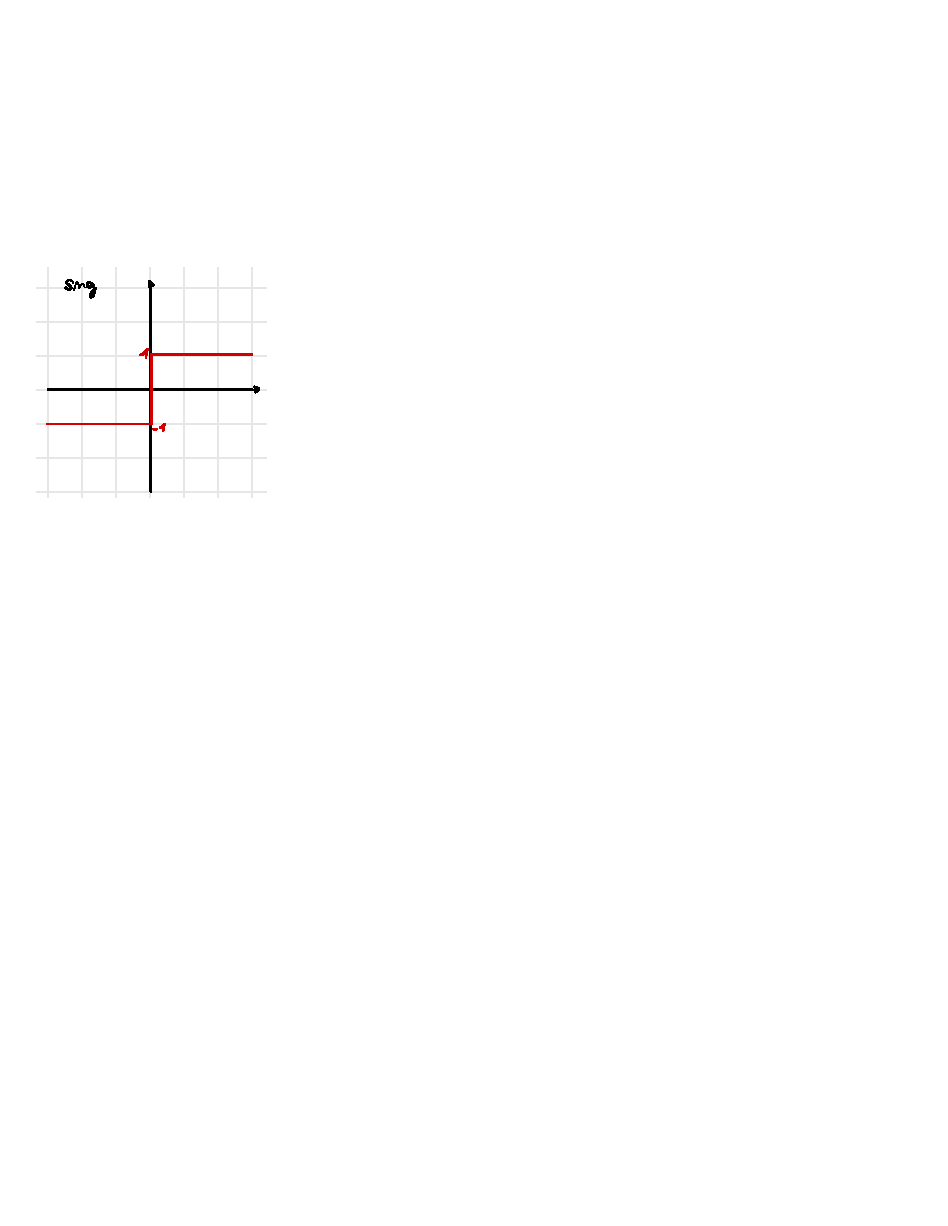
\includegraphics[width=0.4\textwidth]{img/ex_exam/sng_func_2.pdf}
		\caption{Funzione segno $\mathrm{sng}$.}
	\end{figure}

	\noindent
	Si esplicitando le operazioni della funzione:
	
	\begin{equation*}
		f(t) = \mathrm{sgn }\left(a\cdot\cos{\left(\dfrac{2\pi}{T_0} t\right)}\right) = \cos\left(\dfrac{1}{T_0}\cdot 2\pi t\right)
	\end{equation*}

	\noindent
	E si rappresenta inizialmente la funzione $\cos\left(2\pi\right)$ con $T_0 = 1$:
	
	\begin{figure}[!htp]
		\centering
		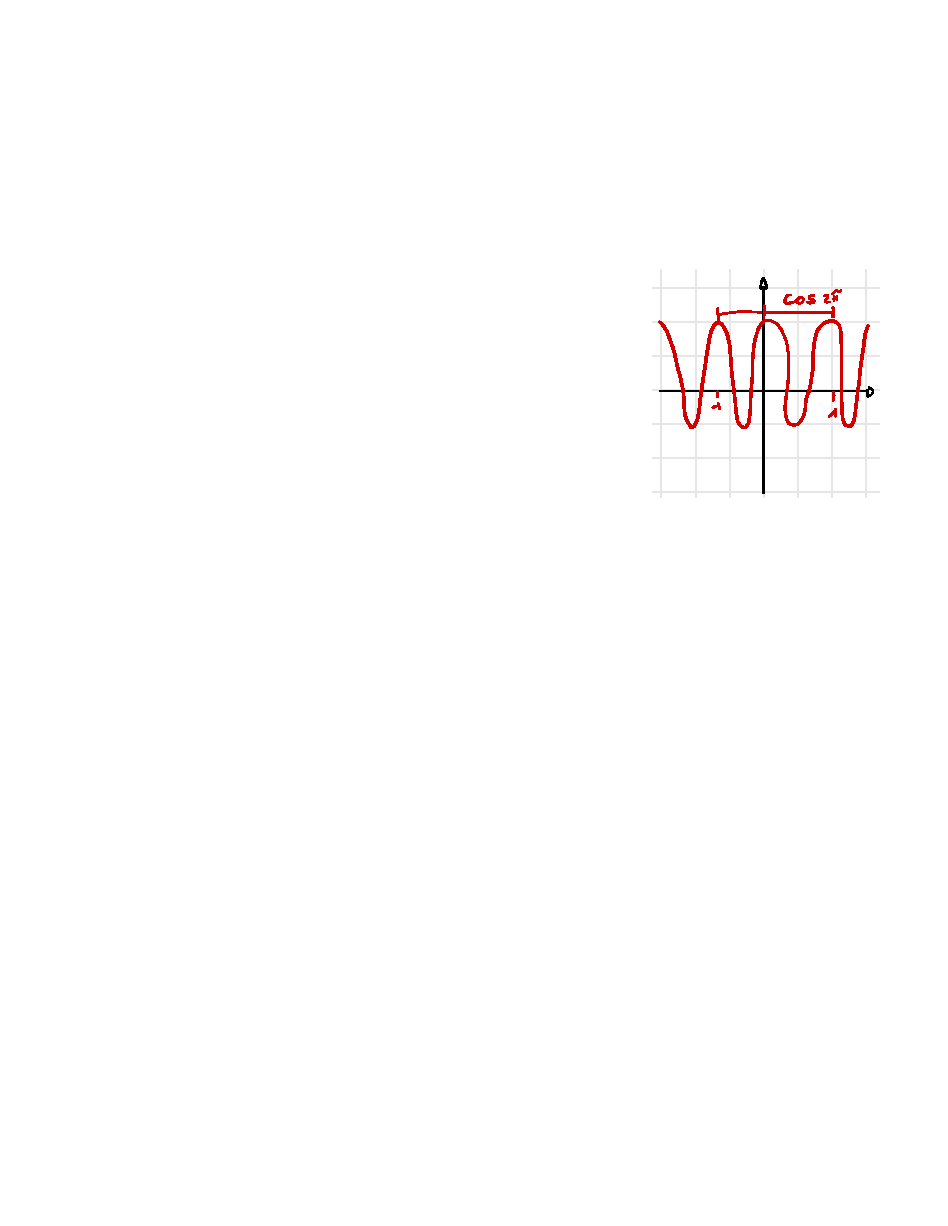
\includegraphics[width=0.4\textwidth]{img/ex_exam/sng_func_2-Mod.pdf}
		\caption{Funzione coseno $\cos\left(2\pi\right)$.}
	\end{figure}

	\newpage

	\noindent
	Si conclude la rappresentazione grafica aumentando $T_0$ in maniera molto semplice:
	
	\begin{figure}[!htp]
		\centering
		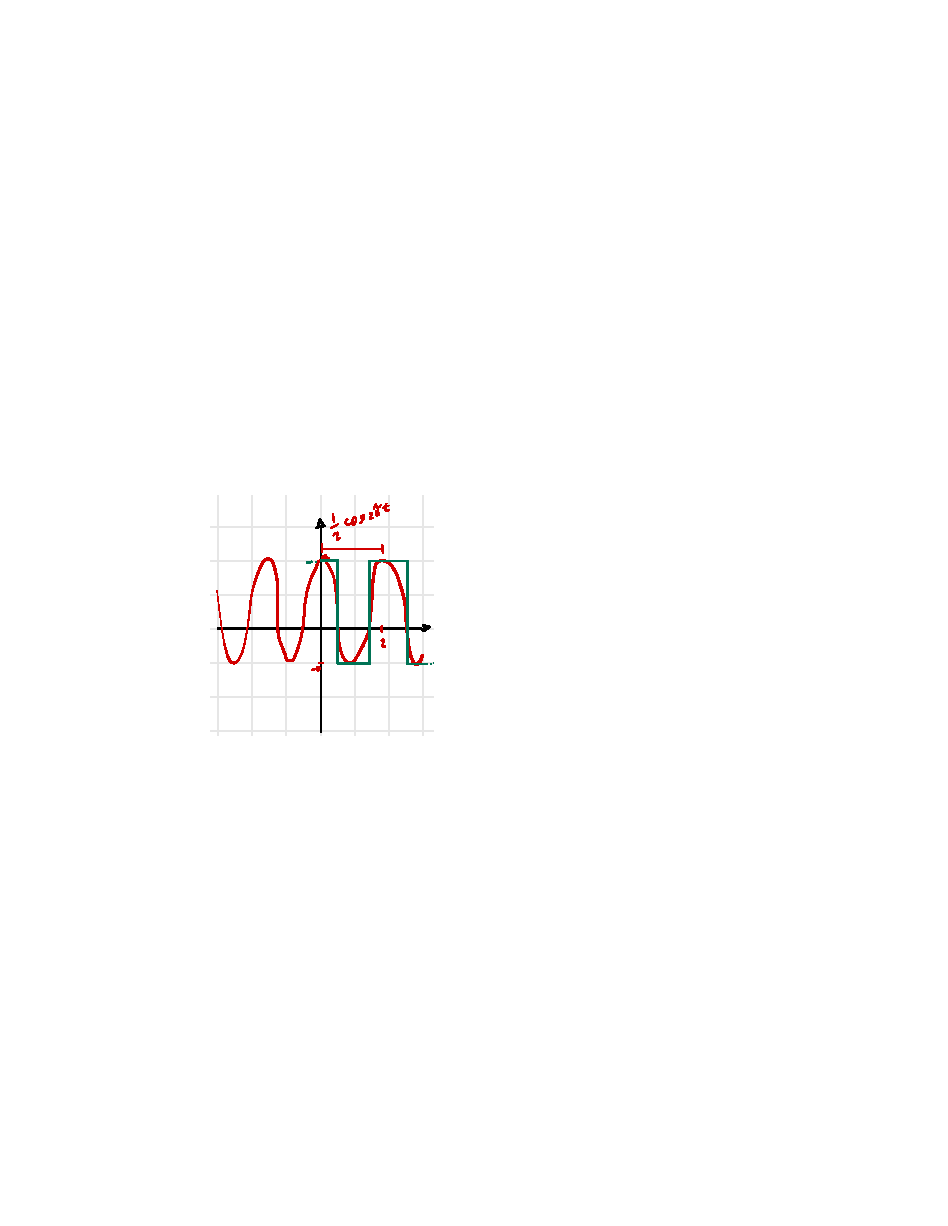
\includegraphics[width=0.4\textwidth]{img/ex_exam/sng_func_2-Mod2.pdf}
		\caption{Funzione coseno $\cos\left(2\pi\right)$ moltiplicata per $\dfrac{1}{T_0}=\dfrac{1}{2}$.}\label{ex2_grafico}
	\end{figure}
	\noindent
	\textcolor{Green4}{\textbf{\emph{Risoluzione II.}}}
	
	\noindent
	Si conclude l'esercizio calcolando l'energia o la potenza del segnale. Per farlo, dato che non è definito in un intervallo ma continua all'infinito, si calcolano i rispettivi integrali in un intervallo arbitrario $n$ e poi lo si estende all'infinito:
	
	\begin{gather*}
		E_{f} = \int_{-\infty}^{\infty} f^{2}(t) \:\mathrm{d}t = \lim_{n\rightarrow\infty} \int_{-n\cdot\frac{T_0}{2}}^{n\cdot\frac{T_0}{2}} f^{2}(t) \:\mathrm{d}t = \lim_{n\rightarrow\infty} n\cdot\int_{-\frac{T_0}{2}}^{\frac{T_0}{2}} f^{2} (t) \:\mathrm{d}t = \infty \\
		P_{f} = \lim_{T\rightarrow\infty} \dfrac{1}{T} \int_{-\frac{T}{2}}^{\frac{T}{2}} f^{2}(t) \:\mathrm{d}t = \lim_{n\rightarrow\infty} \dfrac{1}{nT_{0}} \int_{-n\frac{T_{0}}{2}}^{n\frac{T_{0}}{2}} f^{2}(t)\:\mathrm{d}t = 
		\cancel{\lim_{n\rightarrow\infty}} \dfrac{1}{\cancel{n}T_{0}} \cdot \cancel{n} \cdot \int_{-\frac{T_{0}}{2}}^{\frac{T_{0}}{2}} f^{2}(t)\:\mathrm{d}t = \\
		= \dfrac{1}{T_{0}} \cdot T_{0} = \dfrac{1}{2} \cdot 2 = 1 \longrightarrow \ne 0
	\end{gather*}

	\noindent
	È evidente che il segnale è di potenza. Come si evince dalla figura~\ref{ex2_grafico}, i tratti di colore verde indicano il rettangolo formato dal segnale. Calcolando l'area del rettangolo, si ottiene esattamente il valore di $T_{0}$. Infatti, la base del rettangolo (verticale) è $2$, mentre l'altezza (orizzontale) è $1$.
	
	\newpage
	
	\subsubsection{Cross-Correlazione Normalizzata}\label{cross correlazione normalizzata}
	
	Ha l'\textbf{obbiettivo} di trattare segnali con range di valori diversi e consente di eseguire \textbf{confronti uno-a-molti} (\emph{one-to-many}):
	
	\begin{equation*}
		f_{1} \bar{\otimes} f_{2}\left(t\right) = \dfrac{\displaystyle \int_{-\infty}^{+\infty} \tilde{f_{1}}\left(\tau\right) f_{2}\left(\tau - t\right) \: \mathrm{d}\tau}{\displaystyle \sqrt{E_{f_{1}} E_{f_{2}}}}
	\end{equation*}
	
	\noindent
	In cui $E_{f}$ indica l'\textbf{energia} del segnale $f$. Ci sono due caratteristiche importanti:
	
	\begin{itemize}
		\item $f_{1} \bar{\otimes} f_{2}\left(t\right) \in \left[-1, 1\right]$
		
		\item $\left|f_{1} \bar{\otimes} f_{2}\left(t\right)\right| = 1 \iff f_{1}\left(\tau\right) = \alpha f_{2} \left(\tau - t\right)$
	\end{itemize}
	
	\noindent
	Inoltre, si parla di \textbf{autocorrelazione} (normalizzata e non) quando $f_{1} = f_{2}$. Utile per i segnali stocastici.\newline
	
	\noindent
	Nel \textbf{\emph{caso di segnali discreti}}, dati $x_{1}\left(k\right), x_{2}\left(k\right)$:
	
	\begin{equation*}
		x_{1} \otimes x_{2}\left(n\right) = \sum_{k = -\infty}^{+\infty} \tilde{x_{1}}\left(k\right) x_{2} \left(k - n\right) \hspace{1em} k \in \mathbb{Z}
	\end{equation*}

	\noindent
	Sotto l'ipotesi di convergenza della serie, cioè la serie deve convergere.\newline
	
	\noindent
	Nel caso in cui $x_{1}\left(k\right)$ e $x_{2}\left(k\right)$ sono limitati di lunghezza M ed N rispettivamente, allora la \textbf{cross correlazione è di lunghezza} $M+N-1$.
	
	\newpage
	
	\noindent
	\textcolor{Green4}{\textbf{Cross-Correlazione 1D}}\newline
	
	\noindent
	Data la definizione:
	
	\begin{equation*}
		x_{1} \otimes x_{2}\left(n\right) = \sum_{k = -\infty}^{+\infty} x_{1}\left(k\right) x_{2}\left(k - n\right)
	\end{equation*}
	
	\noindent
	Esistono diverse casistiche:
	
	\begin{itemize}
		\item $n = 0$ si confronta tra $x_{1}$ e $x_{2}$ nei loro domini temporali originali.
		
		\item $n > 0$ sposto $x_{2}$ a destra poiché c'è l'anticipo di $x_{2}$
		
		\item $n < 0$ sposto $x_{2}$ a sinistra poiché c'è ritardo di $x_{2}$
	\end{itemize}

	\begin{figure}[!htp]
		\centering
		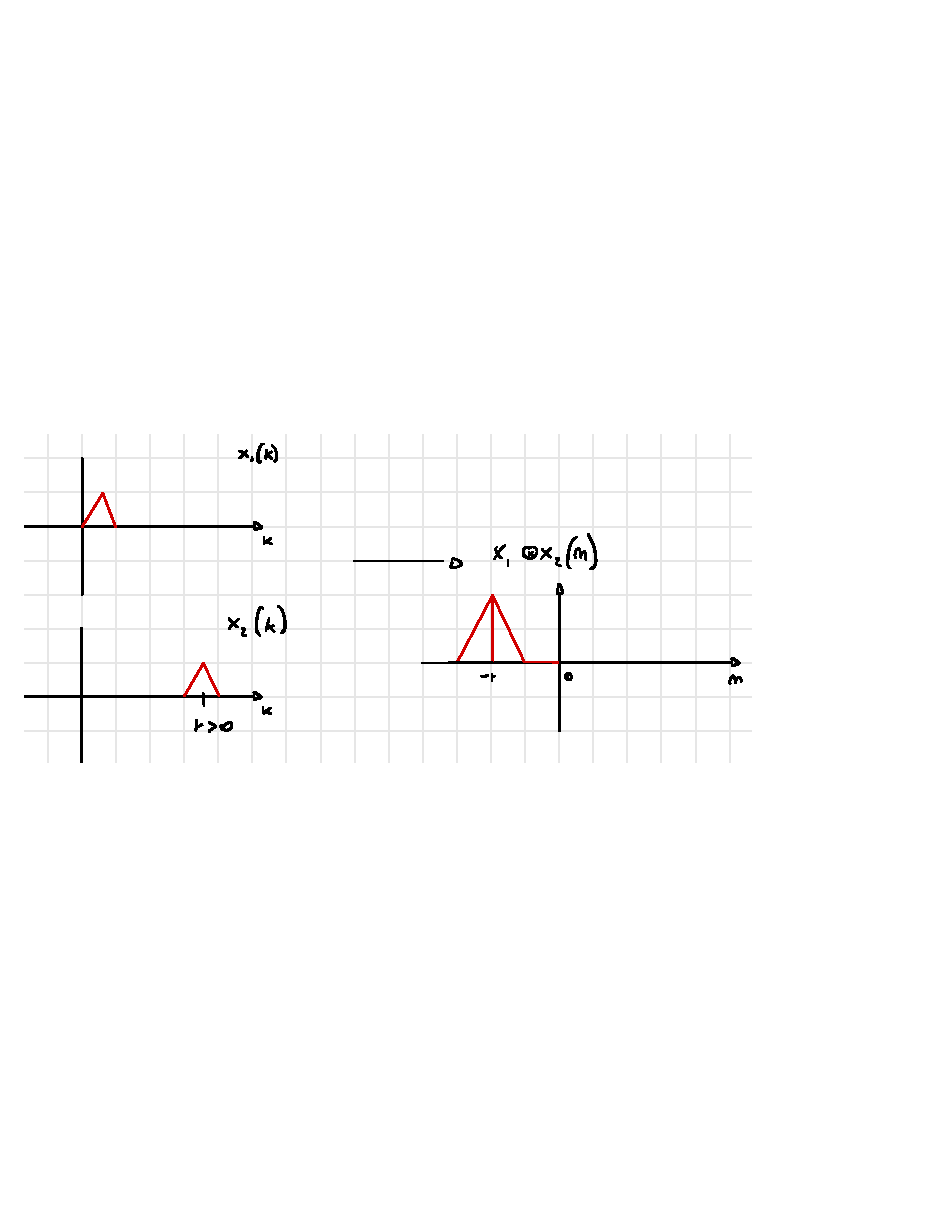
\includegraphics[width=0.9\textwidth]{img/ex_exam/eg_cross-correlazione-1D.pdf}
		\caption{Esempio di cross-correlazione normalizzata 1D.}
	\end{figure}

	\noindent
	Il triangolo $x_{2}$ va verso sinistra e il lasso di tempo che $x_{2}$ non combacia con $x_{1}$, viene rappresentato come una linea orizzontale sull'asse delle $n$ nel piano cartesiano di destra.
	
	\newpage
	
	\noindent
	\textcolor{Green4}{\textbf{Cross-Correlazione 2D}}\newline
	
	\noindent
	Data la definizione:
	
	\begin{equation*}
		x_{1} \otimes x_{2}\left(m, n\right) = \sum_{u = -\infty}^{+\infty} \sum_{v = -\infty}^{+\infty} x_{1}\left(u, v\right) x_{2}\left(u - m, v - n\right) \hspace{1em} u,v,m,n \in \mathbb{Z}
	\end{equation*}
	
	\noindent
	Nel 2D $x_{1}$ e $x_{2}$ possono essere pensate come \textbf{immagini infinite}.\newline
	
	\noindent
	Di solito $x_{1}$ e $x_{2}$ sono \textbf{immagini finite} (segnali digitali ad intervallo limitato), e gli estremi di sommatoria sono quindi finiti.\newline
	
	\noindent
	Il primo segnale $x_{1}$ viene chiamato \textbf{\emph{template}}, o \textbf{\emph{matrice kernel}}, mentre $x_{2}$ genericamente \textbf{immagine} (di solito, la matrice kernel $x_{1}$ ha una dimensionalità minore di quella dell'immagine).\newline
	
	\noindent
	Nel caso $x_{1} = x_{2}$ si ha \textbf{autocorrelazione 2D}.\newline
	
	\noindent
	\textcolor{Green4}{\textbf{Cross-Correlazione normalizzata 2D}}\newline
	
	\noindent
	Si definisce come:
	
	\begin{equation*}
		x_{1} \otimes x_{2}\left(m,n\right) = \dfrac
		{\sum_{u = -\infty}^{+\infty} \sum_{v = -\infty}^{+\infty} \left[x_{1}\left(u, v\right)\right]\left[x_{2}\left(u-m, v-n\right)\right]}
		{\sqrt{\sum_{u = -\infty}^{+\infty} \sum_{v = -\infty}^{+\infty} \left[x_{1}\left(u,v\right)\right]^{2} {\sum_{u = -\infty}^{+\infty} \sum_{v = -\infty}^{+\infty} \left[x_{2}\left(u,v\right)\right]^{2}}}}
	\end{equation*}

	\noindent
	In altre parole, fissato il punto di applicazione $n, m$, si sottrae la media ad ogni punto nell'interno di applicazione dalla matrice kernel. Successivamente, si divide per il prodotto della varianza dei due segnali, estraendo a radice alla fine.
	
	\begin{figure}[!htp]
		\centering
		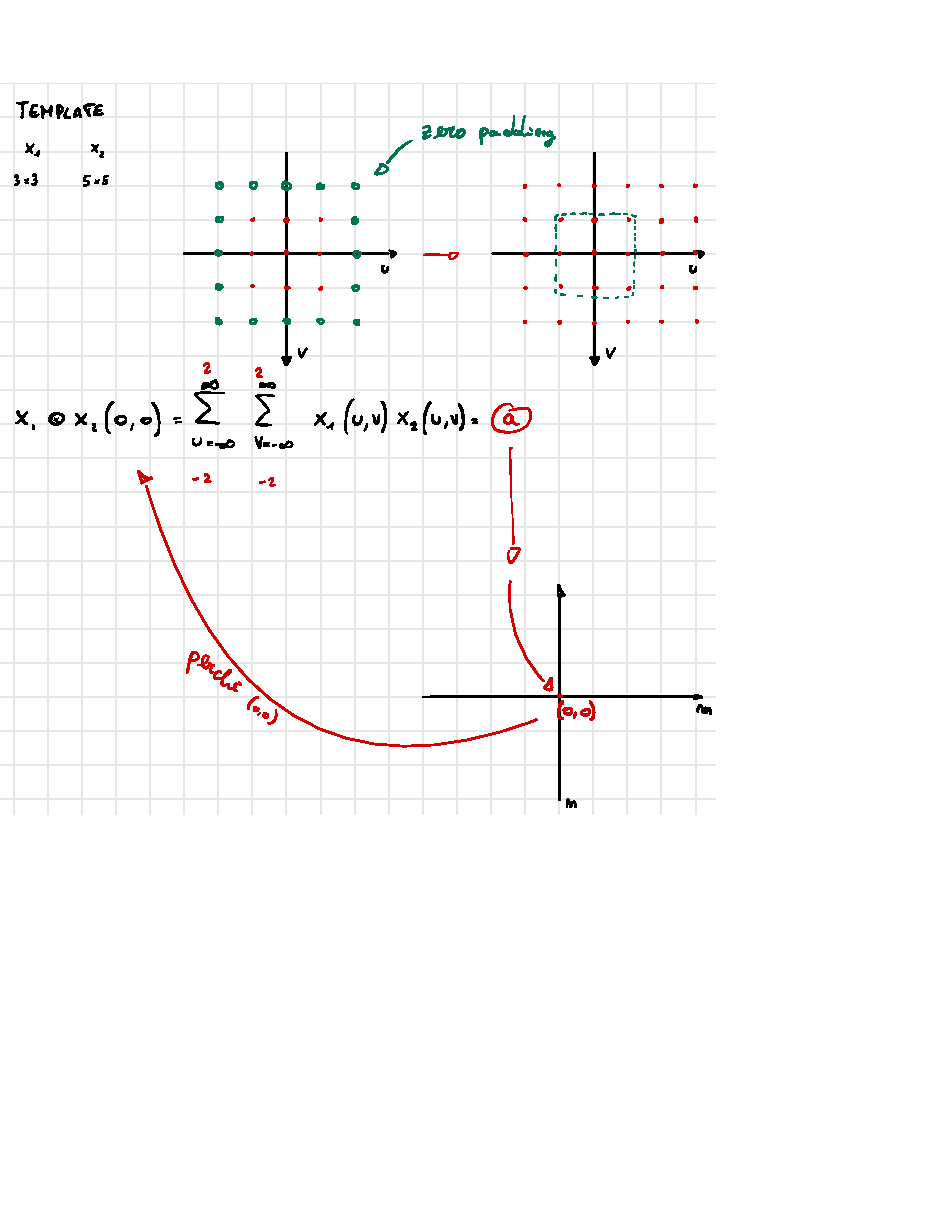
\includegraphics[width=1\textwidth]{img/ex_exam/eg_cross-correlazione-2D.pdf}
		\caption{Esempio di Cross-Correlazione normalizzata 2D.}
	\end{figure}

	\newpage
	
	\noindent
	\textcolor{Red3}{\textbf{Esercizio Cross-Correlazione 2D}}\newline
	
	\noindent
	Dati le due immagini $x_{1}$ di dimensione $5 \times 5$ e $x_{2}$ di dimensione $3 \times 3$, si calcola la cross-correlazione 2D. Quindi, si effettua la rappresentazione grafica.
	
	\begin{figure}[!htp]
		\centering
		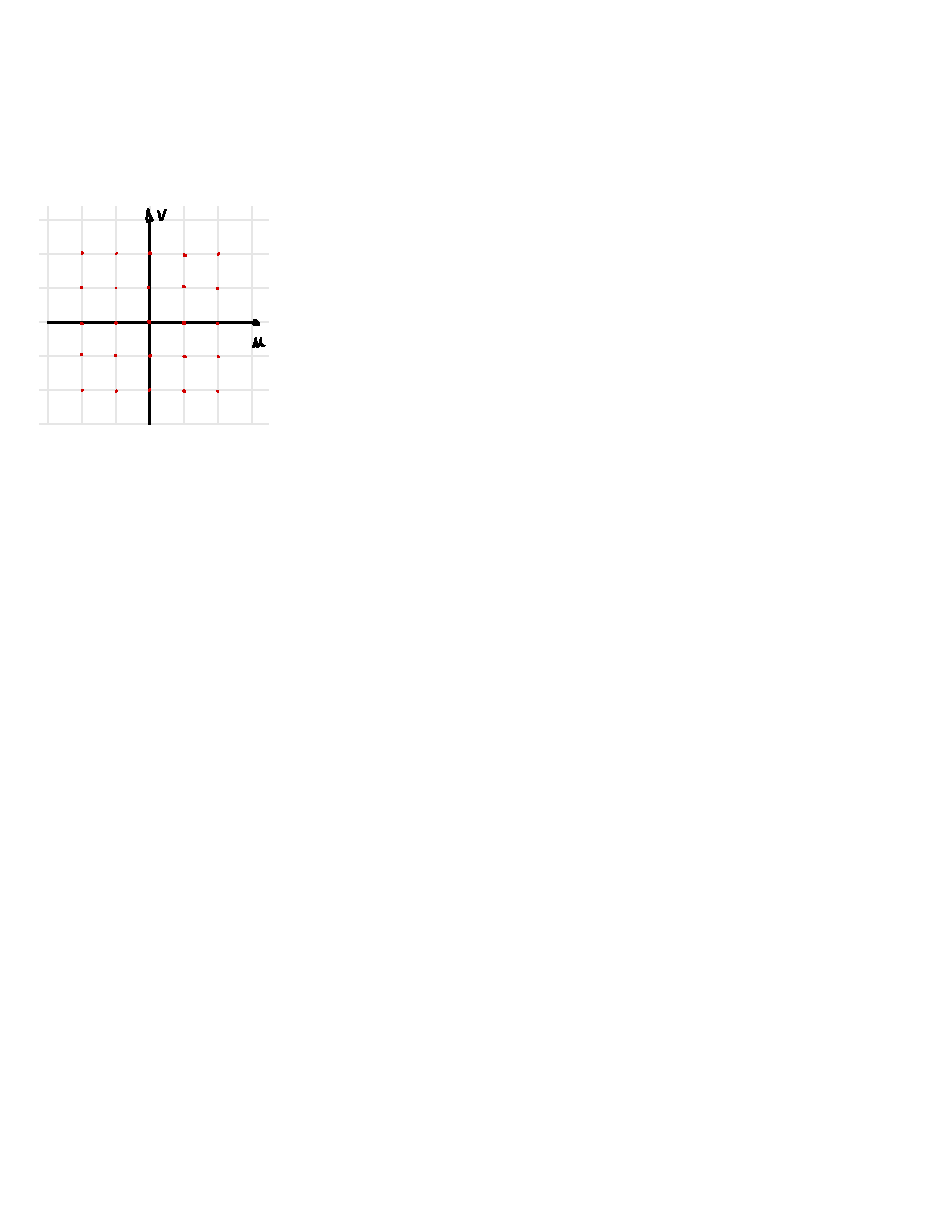
\includegraphics[width=0.5\textwidth]{img/cross-correlazione-2D_ex1.pdf}
		\caption{Piano cartesiano di $x_{2}$ di dimensione $5 \times 5$.}
		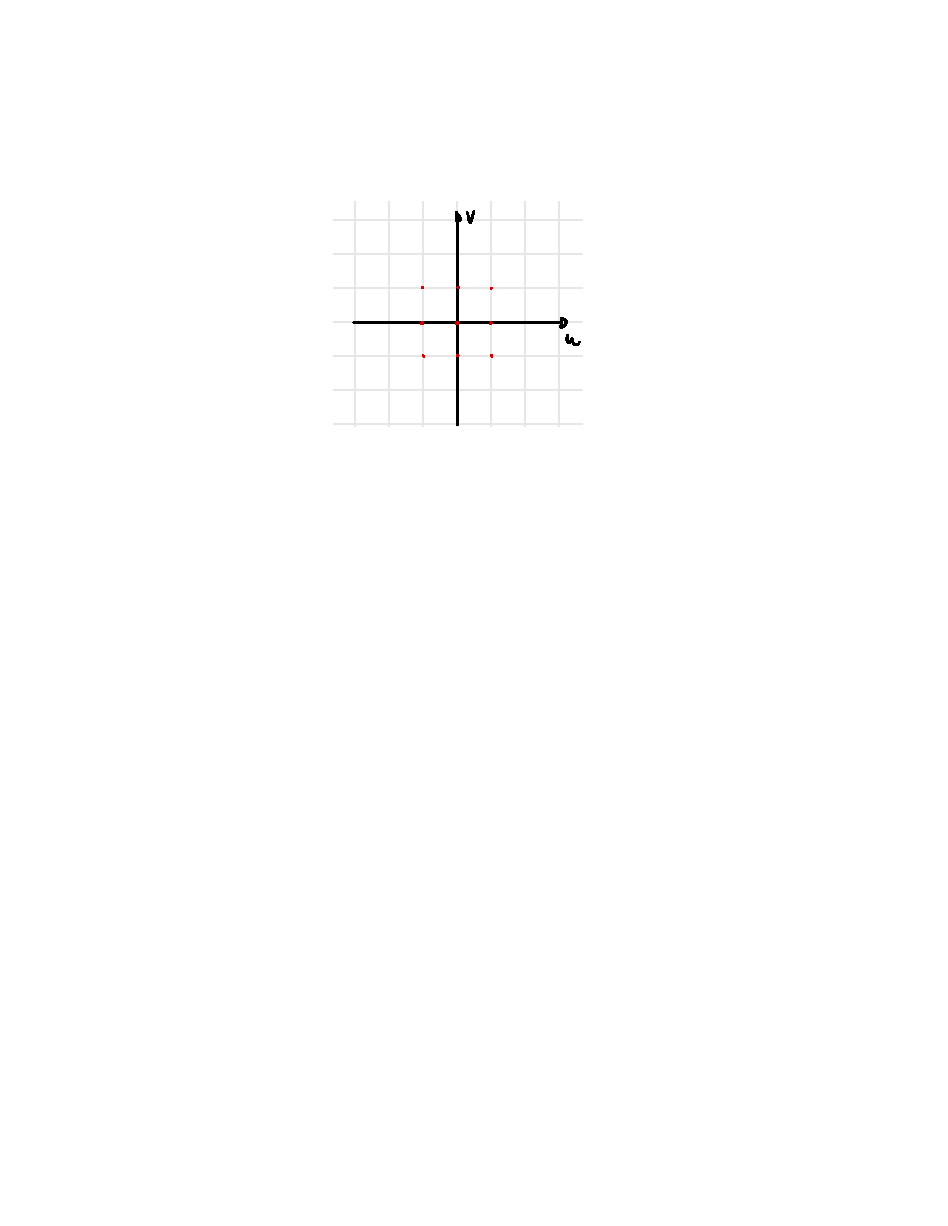
\includegraphics[width=0.5\textwidth]{img/cross-correlazione-2D_ex1_1.pdf}
		\caption{Piano cartesiano di $x_{1}$ di dimensione $3 \times 3$.}
	\end{figure}

	\noindent
	E vengono fornite dall'esercizio le due matrici:
	
	\begin{equation*}
		x_{2} =
		\begin{bmatrix}
			1 & 0 & 0 & 0 & 0 \\
			0 & 1 & 0 & 0 & 0 \\
			0 & 0 & 1 & 0 & 0 \\
			0 & 1 & 1 & 0 & 1 \\
			0 & 0 & 0 & 1 & 0 \\
		\end{bmatrix}
		\hspace{2em}
		x_{1} =
		\begin{bmatrix}
			1 & 0 & 0 \\
			0 & 1 & 0 \\
			0 & 0 & 1 \\
		\end{bmatrix}		
	\end{equation*}

	\noindent
	Esse indicano i valori nei punti corrispondenti. L'\textbf{obbiettivo dell'esercizio} è trovare:
	
	\begin{itemize}
		\item L'argomento massimo della cross-correlazione ($\arg \max x_{1} \otimes x_{2}\left(m,n\right)$);
		
		\item Il massimo della cross-correlazione ($\max x_{1} \otimes x_{2} \left(m,n\right)$).
	\end{itemize}

	\noindent
	L'argomento massimo è con i valori $m = 1$ e $n = -1$ poiché così facendo la diagonale incontra tutti i valori positivi e che formano il massimo. Infatti, prendendo in considerazione la matrice $x_{2}\:5 \times 5$ e osservando l'operazione di cross-correlazione 2D:
	
	\begin{gather*}
		\sum_{u} \sum_{v} x_{1} \left(u,v\right) \cdot x_{2}\left(u - m, v - n\right) \\
		\xrightarrow{\text{sostituzione termini noti } (m, n)} \sum_{u} \sum_{v} x_{1} \left(u,v\right) \cdot x_{2}\left(u - 1, v - \left(-1\right)\right)
	\end{gather*}

	\noindent
	Risulta evidente come si debba spostare a destra, rispetto l'origine, la matrice $x_{2}$ di un solo valore\footnote{Shift a destra poiché $u-1$ nell'equazione rappresenta un ritardo.} e sotto, rispetto sempre l'origine, di un valore negativo\footnote{Spostamento sotto l'asse delle ascisse poiché è un valore positivo $v+1$.}. Così facendo, la diagonale della matrice $x_{2}$ corrisponderà esattamente a tutti i valori $1$ della matrice $x_{1}$.

	\newpage
	
	\subsubsection{Convoluzione}
	
	La \textbf{convoluzione} è un parente stretto della cross-correlazione, ma è leggermente diverso. È definito nel seguente modo:
	
	\begin{equation*}
		f_{1} * f_{2}\left(t\right) = \int_{-\infty}^{+\infty} f_{1}\left(\tau\right) f_{2}\left(t - \tau\right) \mathrm{d}\tau
	\end{equation*}

	\noindent
	Con $t \in \mathbb{R}$. Si ricordi che se i \textbf{segnali non sono né di energia né di potenza, l'integrale \underline{converge}}.\newline
	
	\noindent
	Nel caso in cui i \textbf{segnali} siano \textbf{discreti}, dati $x_{1}\left(n\right)$, $x_{1}\left(n\right)$:
	
	\begin{equation*}
		x_{1} * x_{2} \left(n\right) = \sum_{k = -\infty}^{+\infty} x_{1}\left(k\right) x_{2}\left(n - k\right)
	\end{equation*}

	\noindent
	Con $k \in \mathbb{Z}$.
	
	\noindent
	Nel caso in cui $x_{1} \left(n\right)$ e $x_{2} \left(n\right)$ sono limitati di lunghezza $M$ ed $N$ rispettivamente, allora la \textbf{convoluzione è di lunghezza} $M+N-1$.\newline
	
	\noindent
	\textcolor{Green4}{\textbf{Convoluzione 2D}}\newline
	
	\noindent
	Nel caso delle immagini, quindi del 2D, $x_{1}$ ed $x_{2}$ sono solitamente \textbf{segnali digitali ad intervallo limitato}, e la convoluzione diventa dunque:
	
	\begin{equation*}
		x_{1} * x_{2}\left(m,n\right) = \sum_{u = -\infty}^{+\infty} \sum_{v = -\infty}^{+\infty} x_{1} \left(u,v\right) x_{2}\left(m - u, n - v\right) \hspace{2em} u,v,m,n\in\mathbb{Z}
	\end{equation*}

	\noindent
	Solitamente il primo segnale $x_{1}$ viene chiamato \textbf{\underline{filtro}}, o \textbf{\underline{matrice kernel}}, mentre $x_{2}$ genericamente \textbf{\underline{immagine}} (solitamente la matrice kernel ha una dimensione inferiore di quella dell'immagine).
	
	\newpage
	
	\section{Analisi di Fourier}
	
	\subsection{Serie di Fourier}\label{serie di fourier}
	
	Una funzione, chiamata \textbf{\underline{funzione di sintesi}}, $f: \mathbb{R} \rightarrow \mathbb{R}$ di variabile continua $t$, periodica di periodo $T$, si esprime come:
	
	\begin{equation*}
		f(t) = \sum_{n = -\infty}^{+\infty} c_{n} \underbrace{e^{j \frac{2\pi n}{T}t}}_{\text{fasore}} \hspace{2em} n\in\mathbb{Z}
	\end{equation*}

	\noindent
	Dove $c_{n}$ è un numero complesso. Invece, una \textbf{\underline{funzione di analisi}} è espressa come:
	
	\begin{equation*}
		c_{n} \in \mathbb{C} = \dfrac{1}{T} \int_{-\frac{T}{2}}^{+\frac{T}{2}} f\left(t\right) \underbrace{e^{-j \frac{2\pi n}{T}t}}_{\text{fasore}} \mathrm{d}t \hspace{2em} n \in \mathbb{Z}
	\end{equation*}

	\noindent
	\textbf{N.B.} si ricorda che $e^{j \frac{2\pi n}{T}t}$ è un \textbf{fasore rotante} di velocità angolare $\dfrac{2\pi n}{T} t$.\newline
	La \textbf{\underline{funzione di sintesi}} quindi non è altro che una somma di infiniti termini. Ciascuno è composto dalla moltiplicazione tra un numero complesso ed un fasore, il quale \emph{produce un altro fasore}. Esprimendo $c_{n}$ come numero complesso in forma polare:
	
	\begin{equation*}
		c_{n} e^{j \frac{2 \pi n}{T} t} = |c_{n}| e^{j \theta_{n}} e^{j \frac{2 \pi n}{T} t} = |c_{n}| e^{j \left(\frac{2 \pi n}{T} t + \theta_{n}\right)}
	\end{equation*}

	\noindent
	Si può notare come questa conversione corrisponda ad \textbf{estendere} il fasore $e^{j\frac{2 \pi n}{T} t}$ ad una lunghezza $|c_{n}|$ facendolo partire con un \textbf{angolo di partenza} uguale a $\theta_{n}$ (chiamato \textbf{\underline{angolo di fase}}).\newline
	
	\noindent
	\textbf{\underline{Altra osservazione:}} se $c_{n}$ appartiene all'insieme $\mathbb{R}$, significa che $\theta_{n}$ non compare. Questo comporta un cambiamento nella lunghezza dell'$n$-esimo fasore pari a $|c_{n}|$:
	
	\begin{equation*}
		c_{n} = |c_{n}| \cancel{e^{j \theta_{n}}}
	\end{equation*}

	\newpage
	
	\noindent
	\textcolor{Green4}{\textbf{\underline{Esempio 1}}}\newline
	
	\noindent
	Il primo esempio di serie di Fourier si applica per il segnale trigonometrico:
	
	\begin{equation*}
		f\left(t\right) = \cos\left(2 \pi t\right) \hspace{2em} \text{con } T = 1
	\end{equation*}

	\noindent
	Applicando la \textbf{funzione di analisi} e saltando i passaggi perché complessi, si ottengono i seguenti valori:
	
	\begin{equation*}
		c_{-1} = \dfrac{1}{2} \hspace{3em}
		c_{0} = 0 \hspace{3em}
		c_{1} = \dfrac{1}{2} \hspace{3em}
		c_{i \le -2, i \ge 2} = 0
	\end{equation*}

	\noindent
	E sostituendo nella \textbf{funzione di sintesi}:
	
	\begin{equation*}
		\cos\left(2 \pi t\right) = \dfrac{1}{2} e^{-j 2 \pi t} + \dfrac{1}{2} e^{j 2 \pi t} = \dfrac{e^{j 2 \pi t} + e^{-j 2 \pi t}}{2}
	\end{equation*}

	\noindent
	Ci sono \textbf{tre osservazioni} da fare:
	
	\begin{enumerate}[label=\Roman*.]
		\item $\dfrac{2\pi}{T} = f_{0}$;
		
		\item $c_{n} = |c_{n}| e^{j\theta_{n}}$;
		
		\item In questo caso, $c_{n} \in \mathbb{R}$ quindi l'angolo di fase non è presente.
	\end{enumerate}

	\noindent
	\textbf{Le parti} dell'equazione sono le seguenti:
	
	\begin{equation*}
		\cos{\left(2 \pi t\right)} = \dfrac{1}{2} e^{-j 2 \pi t} + \dfrac{1}{2} e^{j 2 \pi t}
	\end{equation*}

	\begin{itemize}[label=\ding{43}]
		\item $\cos{\left(2 \pi t\right)} \rightarrow$ La funzione trigonometrica da studiare
		
		\item $\dfrac{1}{2} e^{-j 2 \pi t} \rightarrow$ Fasore di modulo $0.5$ e velocità angolare $-2\pi t$
		
		\item $\dfrac{1}{2} e^{j 2 \pi t} \rightarrow$ Fasore di modulo $0.5$ e velocità angolare $2\pi t$
	\end{itemize}

	\begin{figure}[!htp]
		\centering
		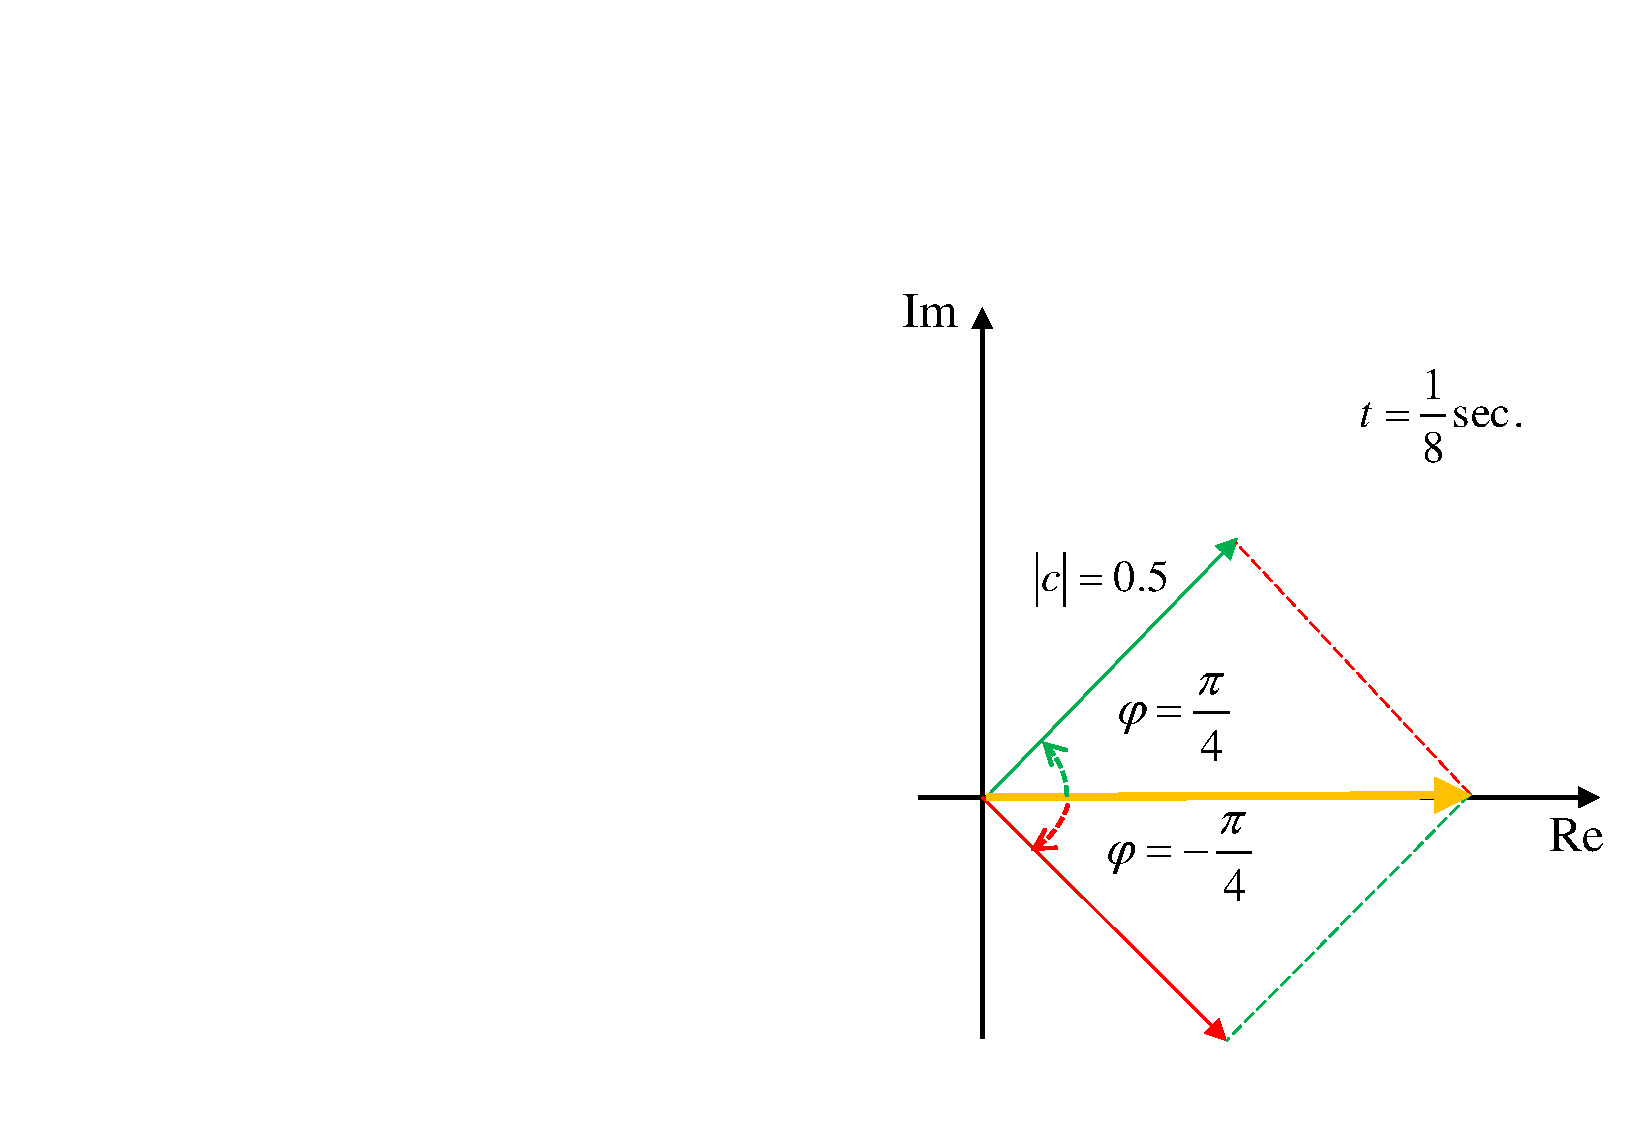
\includegraphics[width=0.5\textwidth]{img/fourier_eg1.pdf}
		\caption{Grafico rappresentante i due fasori. La freccia verde rappresenta il valore assunto da $\cos{\left(2\pi t\right)}$ per $t = \dfrac{1}{8}$.}
	\end{figure}

	\noindent
	I coefficienti $c_{n = -1}$ e $c_{n = 1}$ sono relativi ai \textbf{\underline{moduli o ampiezze}} \textbf{dei fasori} complessi di frequenza $f_{0} \cdot n$ con $n = -1,1$ e ricordando che:
	
	\begin{equation*}
		\exp\left(j \left(\dfrac{2 \pi n}{T} t\right)\right) = \exp\left(j \left(f_{0} n t\right)\right)
	\end{equation*}

	\noindent
	Che si possono annotare con le variabili $f_{-1}$ e $f_{1}$ per $f_{0} \cdot n$ con $n = -1, 1$ e analogamente per gli altri $n \in \mathbb{Z}$.\newline
	
	\noindent
	Inoltre, è possibile disegnare lo \textbf{\underline{spettro di ampiezza}} che \textbf{mostra i moduli dei fasori costruiti con la trasformata di Fourier}, in particolare la funzione di sintesi.
	
	\begin{figure}[!htp]
		\centering
		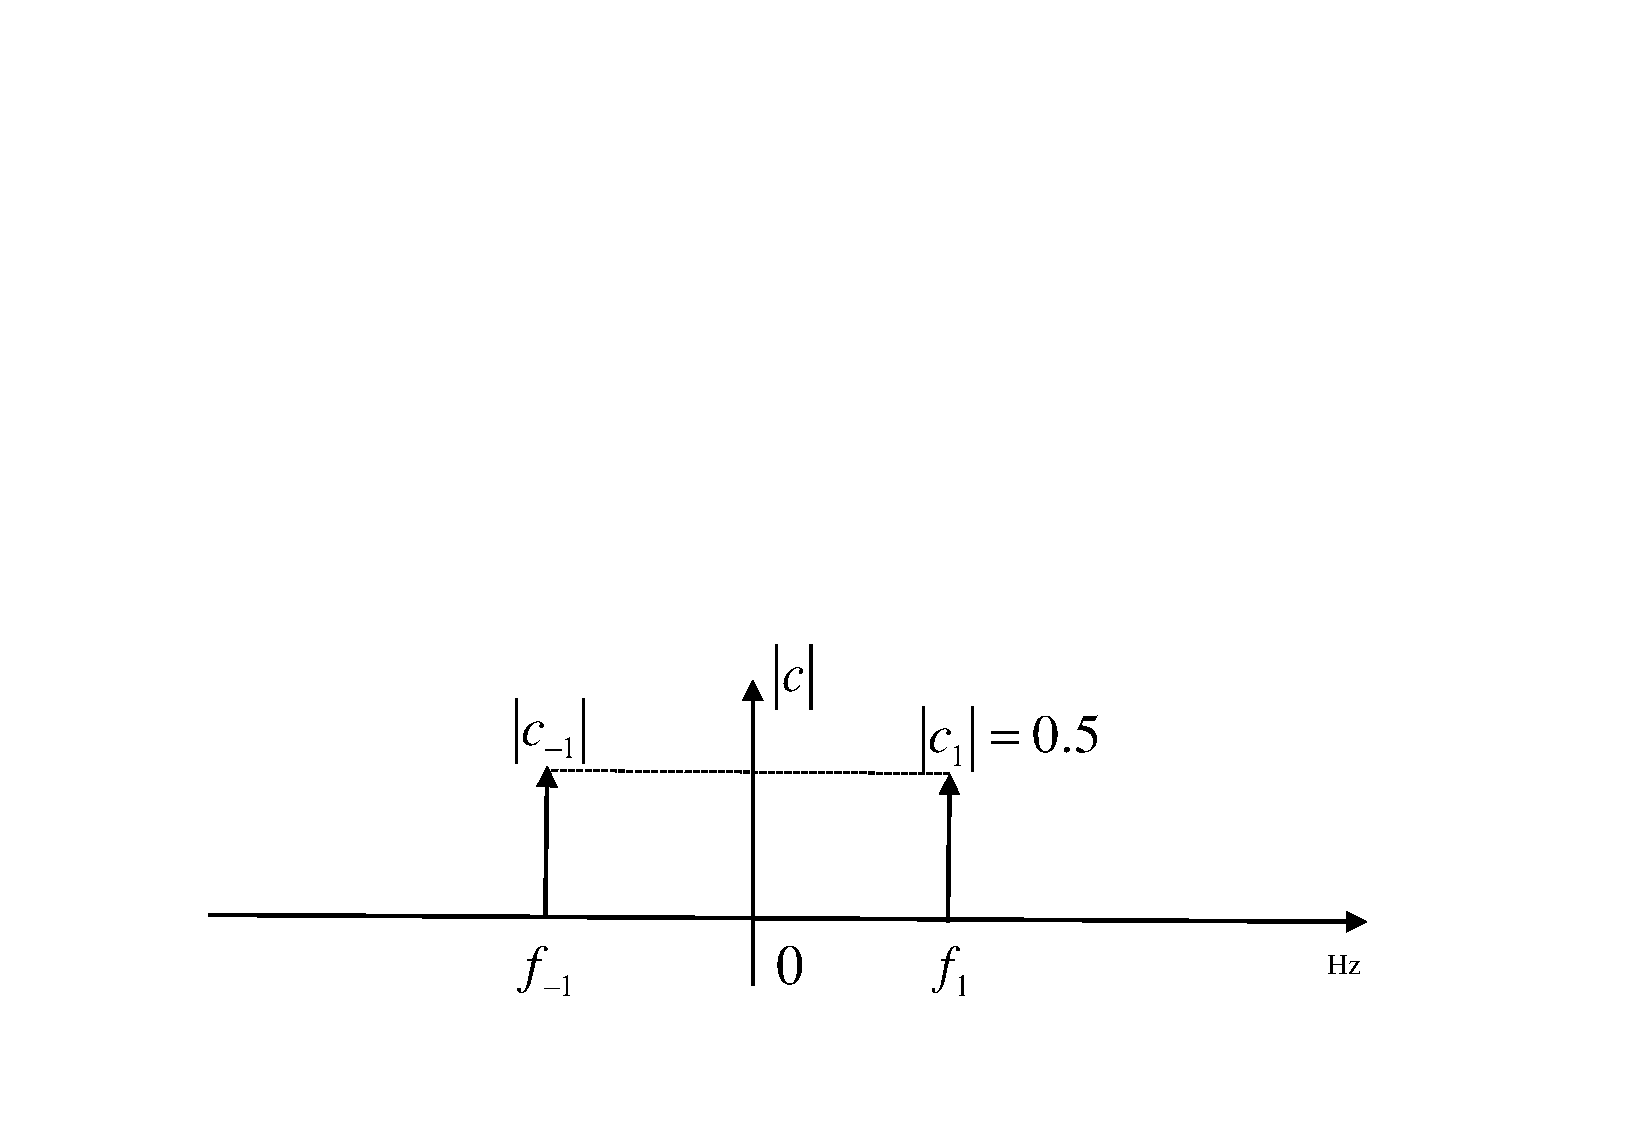
\includegraphics[width=0.9\textwidth]{img/fourier_spettro_di_ampiezza.pdf}
		\caption{Grafico che rappresenta lo spettro di ampiezza.}
	\end{figure}

	\newpage
	
	\noindent
	\textcolor{Green4}{\textbf{\underline{Esempio 2}}}\newline
	
	\noindent
	Il secondo esempio di serie di Fourier è il segnale trigonometrico:
	
	\begin{equation*}
		f\left(t\right) = \sin\left(2 \pi t\right) \hspace{2em} \text{con } T = 1
	\end{equation*}

	\noindent
	Applicando la \textbf{funzione di analisi} e saltando i passaggi perché complessi, si ottengono i seguenti valori:
	
	\begin{equation*}
		c_{-1} = -\dfrac{1}{2j} \hspace{3em}
		c_{0} = 0 \hspace{3em}
		c_{1} = \dfrac{1}{2j} \hspace{3em}
		c_{i \le -2, i \ge 2} = 0
	\end{equation*}

	\noindent
	Dove questa volta $c_{n} \in \mathbb{C}$ ed in particolare:
	
	\begin{equation*}
		\pm \dfrac{1}{2j} = \pm \dfrac{1}{2j} \cdot \dfrac{j}{j} = \pm \dfrac{1}{2} \cdot \dfrac{j}{j^{2}} = j \cdot \mp \dfrac{1}{2}
	\end{equation*}

	\noindent
	Si passa alla forma di esponenziale complesso:
	
	\begin{gather*}
		j \cdot \dfrac{1}{2} = 0 + j \cdot \dfrac{1}{2} \\
		|c| = \sqrt{0^{2} + \left(\dfrac{1}{2}\right)^{2}} = \dfrac{1}{2} \\
		\theta = \arctan\left(\dfrac{0.5}{0}\right) \rightarrow \dfrac{\pi}{2} \\
		\dfrac{1}{2} e^{j \cdot \frac{\pi}{2}} = c_{-1}
	\end{gather*}

	\begin{figure}[!htp]
		\centering
		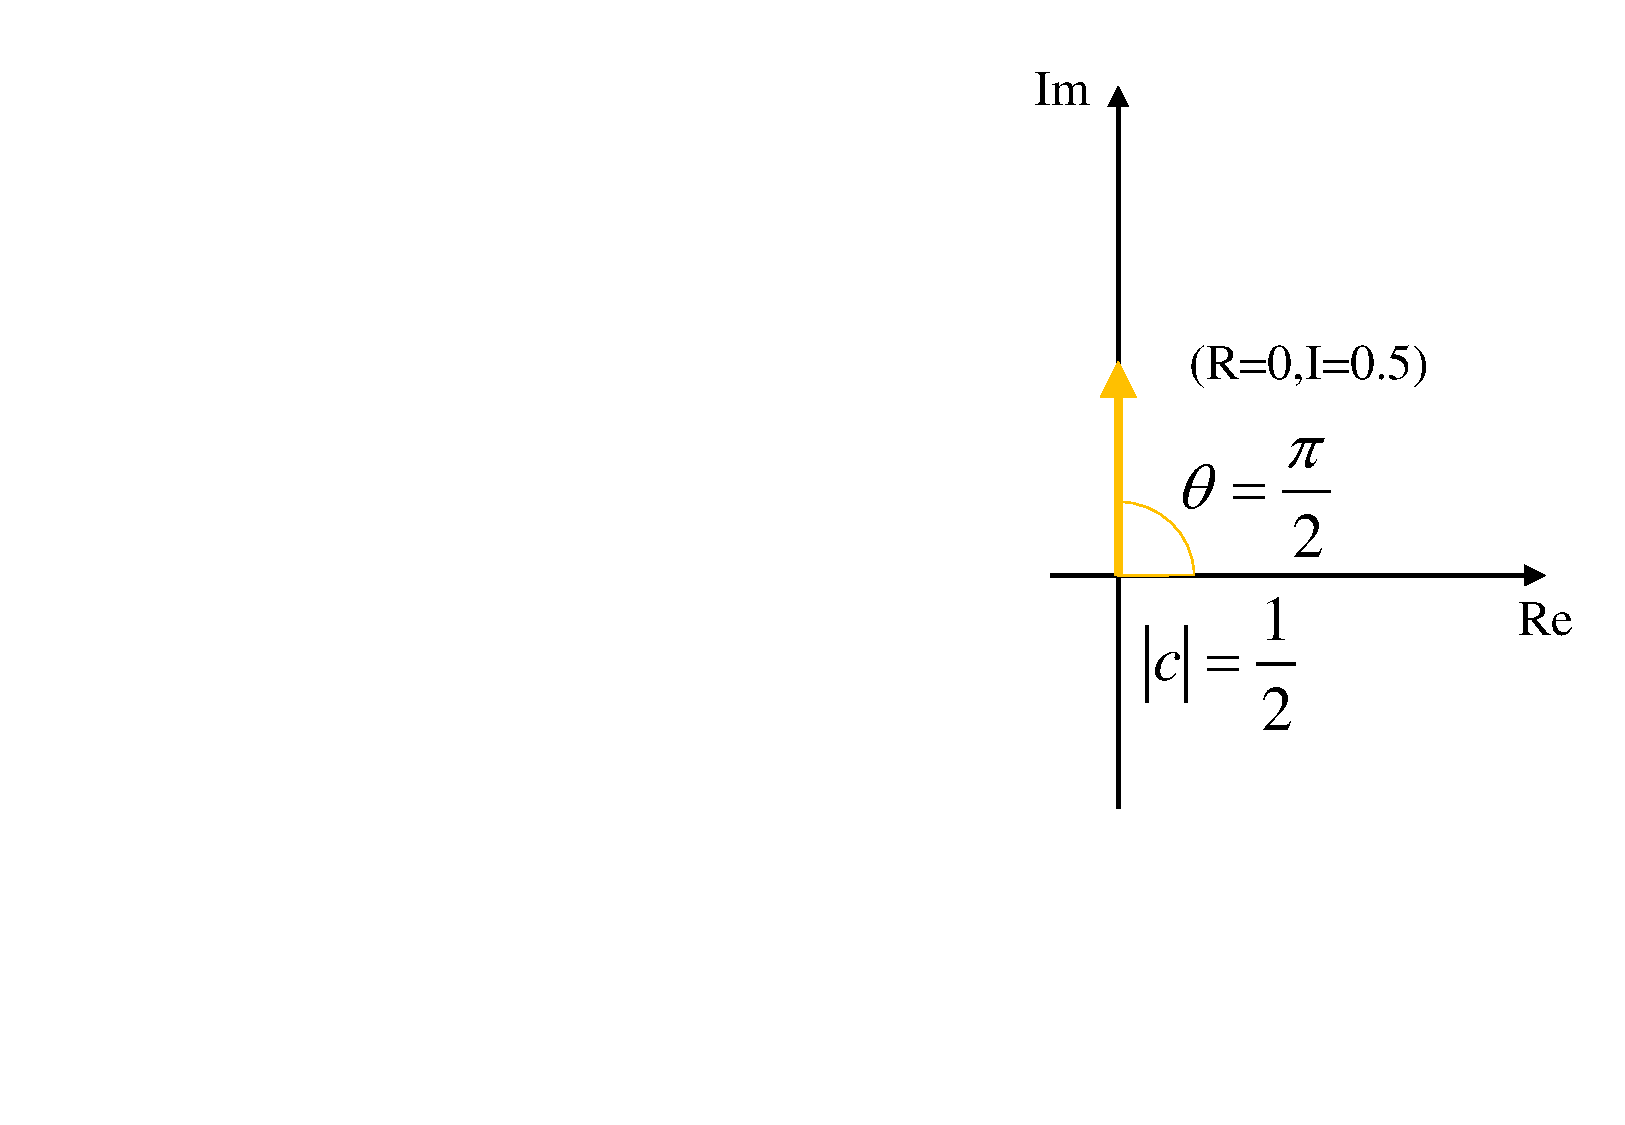
\includegraphics[width=0.3\textwidth]{img/fourier_eg2.pdf}
		\caption{Grafico di $c_{-1}$.}
	\end{figure}

	\newpage
	\noindent
	Analogamente:
	
	\begin{gather*}
		j \cdot -\dfrac{1}{2} = 0 + j \cdot \left(-\dfrac{1}{2}\right) \\
		|c| = \sqrt{0^{2} + \left(-\dfrac{1}{2}\right)^{2}} = \dfrac{1}{2} \\
		\theta = \arctan\left(-\dfrac{0.5}{0}\right) \rightarrow -\dfrac{\pi}{2} \\
		\dfrac{1}{2} e^{j \cdot \left(-\frac{\pi}{2}\right)} = c_{1}
	\end{gather*}

	\begin{figure}[!htp]
		\centering
		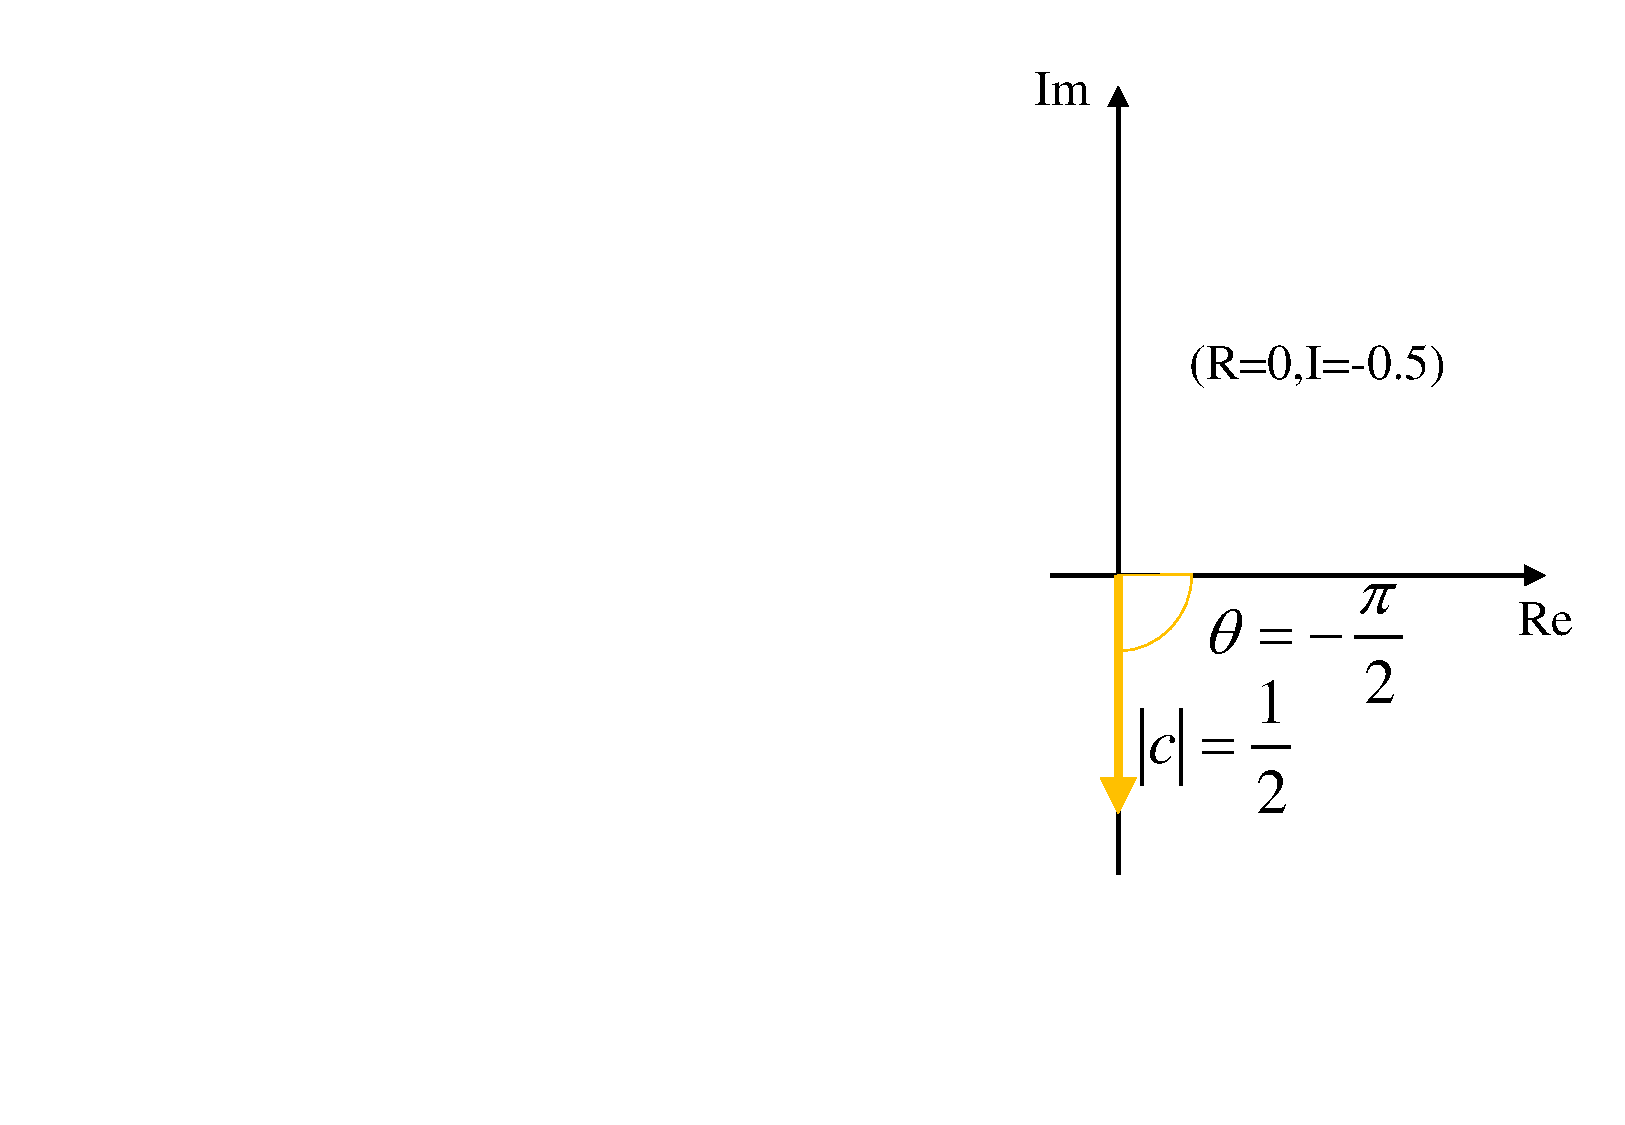
\includegraphics[width=0.3\textwidth]{img/fourier_eg2_2.pdf}
		\caption{Grafico di $c_{1}$.}
	\end{figure}

	\newpage
	\noindent
	Applicando l'\textbf{equazione di sintesi} e sostituendo i termini noti:
	
	\begin{gather*}
		\sin{\left(2 \pi t\right)} = \sum_{n = -\infty}^{+\infty} c_{n} e^{j \frac{2 \pi n}{T} t} = c_{-1} e^{j-2\pi t} + c_{1} e^{j2\pi t} \\
		\xrightarrow{\text{sostituzione dei termini noti }c_{-1}, c_{1}} = \dfrac{1}{2} e^{j \frac{\pi}{2}} e^{j \cdot \left(-2 \pi t\right)} + \dfrac{1}{2}  e^{j \frac{-\pi}{2}} e^{j 2 \pi t} \\
		\xrightarrow{\text{forma finale }} = \dfrac{1}{2} \exp{\left(j\left(-2 \pi t + \dfrac{\pi}{2}\right)\right)} + \exp{\left(j\left(2 \pi t - \dfrac{\pi}{2}\right)\right)}
	\end{gather*}

	\begin{figure}[!htp]
		\centering
		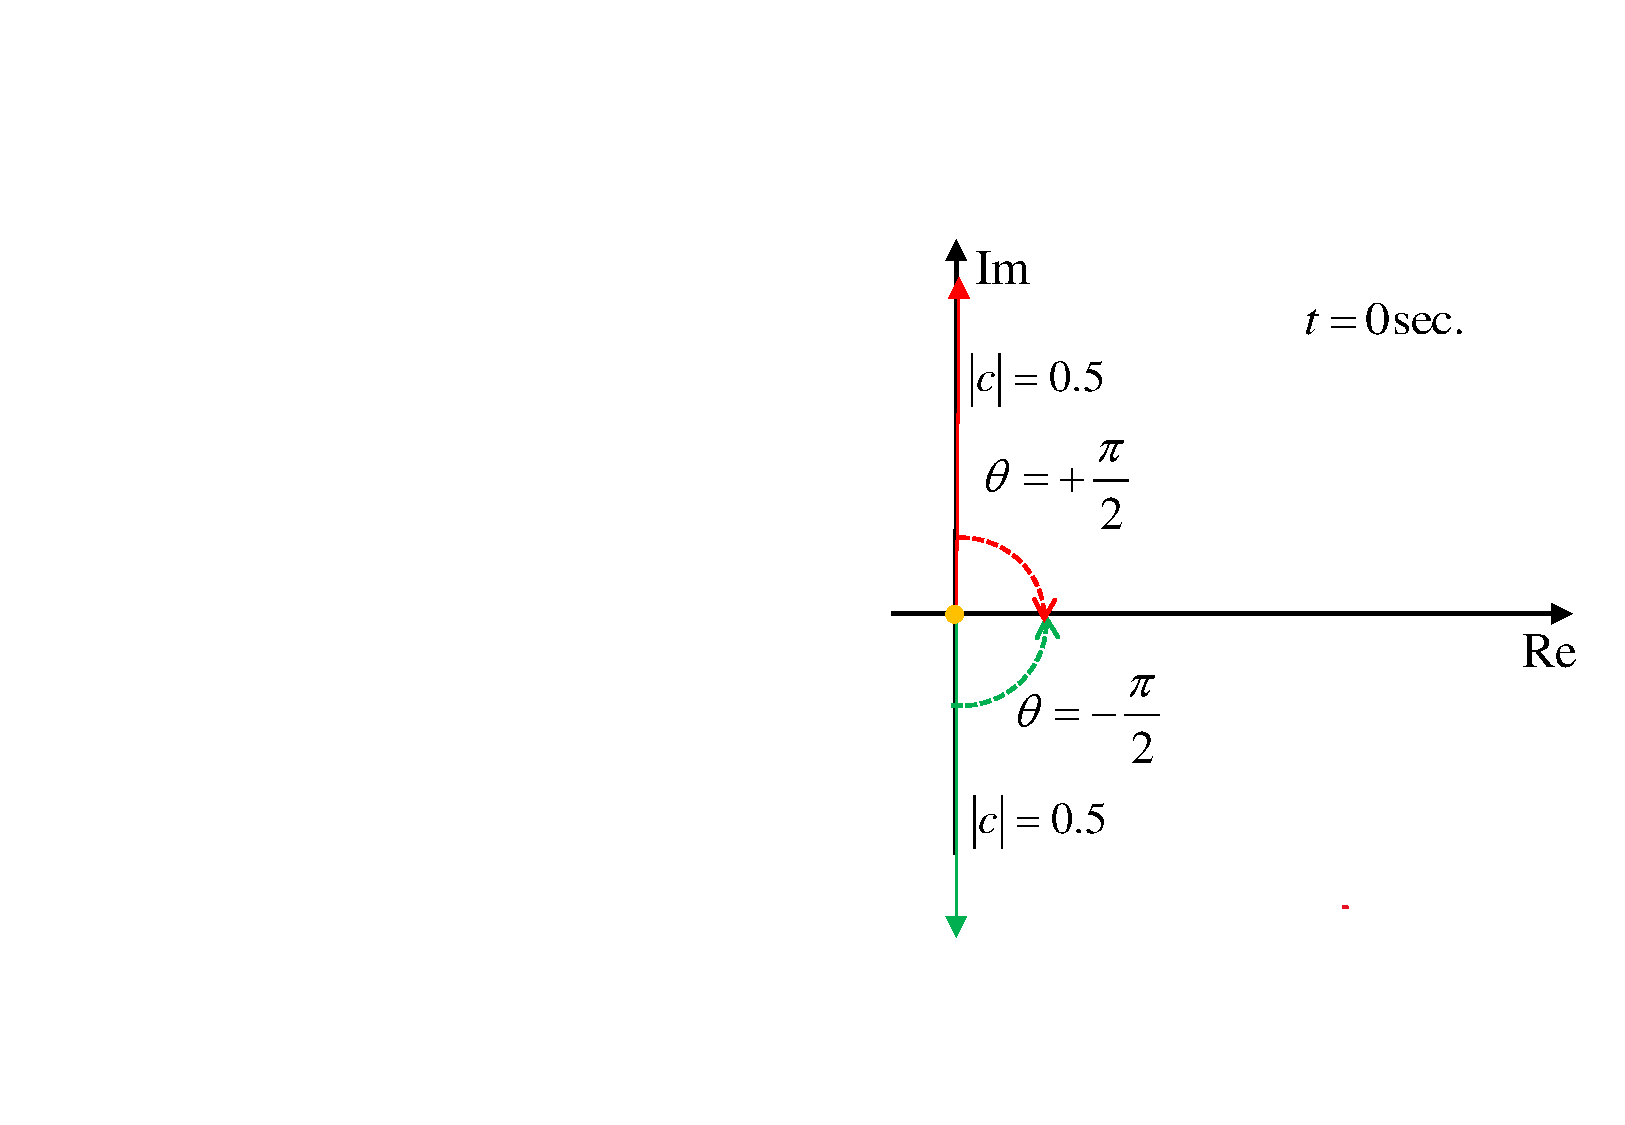
\includegraphics[width=0.5\textwidth]{img/fourier_eg2_3.pdf}
		\caption{Grafico finale.}
	\end{figure}

	\noindent
	Infine, si disegna lo \textbf{\underline{spettro di ampiezza}} e lo \textbf{\underline{spettro di fase}}, quest'ultimo è un \textbf{grafico in cui si riportano gli angoli di fase della funzione}.
	
	\begin{figure}[!htp]
		\centering
		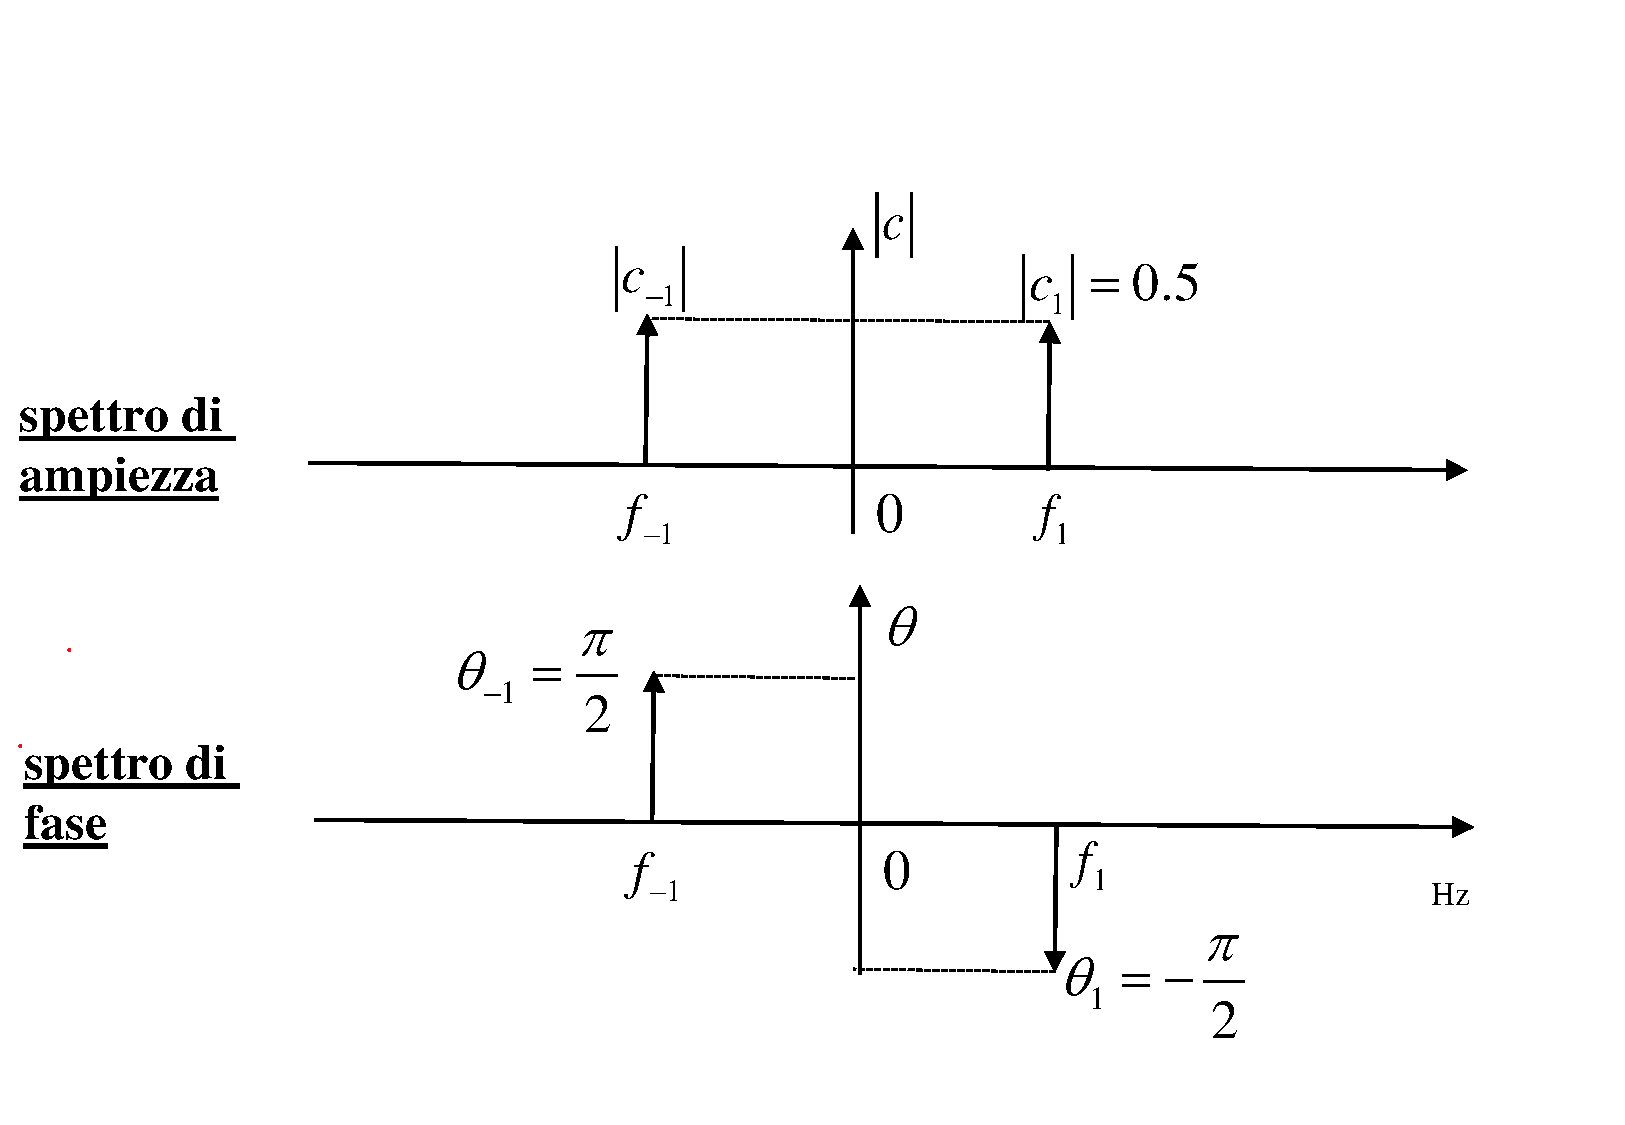
\includegraphics[width=0.9\textwidth]{img/fourier_spettro_di_ampiezza-e-fase.pdf}
		\caption{Spettro di ampiezza e di fase della funzione $\sin\left(2 \pi t\right)$.}
	\end{figure}

	\newpage
	
	\subsubsection{Proprietà della serie di Fourier}
	
	\noindent
	Lo \textbf{spettro di ampiezza e di fase} sono funzioni nel dominio delle frequenze che formano lo {\underline{\textcolor{Red3}{\textbf{spettro di Fourier}}}}. Lo spettro di Fourier per i segnali periodici gode delle \textbf{seguenti \underline{proprietà}}:
	
	\begin{itemize}
		\item Lo \textbf{spettro di ampiezza è \emph{simmetrico}} rispetto all'asse $y$;
		
		\item Lo \textbf{spettro di fase è \emph{antisimmetrico}} rispetto all'asse $y$;
		
		\item Se i coefficienti $c_{n}$ sono reali, \textbf{non esiste lo spettro di fase};
		
		\item Entrambe gli spettri sono funzioni a pettine\label{funzioni a pettine}, definite su frequenze multiple rispetto a quella fondamentale:
		
		\begin{equation*}
			\left\{\dfrac{2 \pi n}{T}\right\}_{n \in \mathbb{Z}} = \left\{f_{0} \cdot n\right\}_{n \in \mathbb{Z}} \equiv \left\{f_{n}\right\}_{n \in \mathbb{Z}}
		\end{equation*}
	\end{itemize}

	\newpage
	
	\subsection{Trasformata di Fourier continua} \label{trasformata di fouerier continua}
	
	\subsubsection{Trasformata di Fourier}
	
	Sia $f\left(t\right)$ un \textbf{segnale reale continuo} $f:\mathbb{R} \rightarrow \mathbb{R}$ periodico o non, si definisce la \textcolor{Red3}{\textbf{Trasformata di Fourier}} (TdF) $\mathcal{F}\left(f\left(t\right)\right) = F\left(\mu\right)$ il segnale $\mathcal{F}: \mathbb{R} \rightarrow \mathbb{C}$:
	
	\begin{equation*}
		\mathcal{F}\left(f\left(t\right)\right) = F\left(\mu\right) = \int_{-\infty}^{+\infty} f\left(t\right) e^{-j 2 \pi \mu t} \: \mathrm{d}t
	\end{equation*}

	\noindent
	L'\textbf{unità frequenziale} $\mu$ è l'angolo di $\frac{n}{T}$ della serie di Fourier (per esempio, con $n = 1$, $T = 1$ sec. $\rightarrow \mu = 1 \text{ sec.}^{-1} = 1$ Hz).\newline
	
	\noindent
	La Trasformata di Fourier esiste se $f\left(t\right)$ è un \textbf{segnale di energia}. Condizione sufficiente e non necessaria perché altri segnali ammettono la TdF.
	
	\subsubsection{Trasformata di Fourier inversa}
	
	Sia $F\left(\mu\right)$ la trasformata di Fourier di un segnale $f: \mathbb{R} \rightarrow \mathbb{R}$. Si definisce la \textcolor{Red3}{\textbf{trasformata di Fourier inversa}} il segnale $\mathcal{F}^{-1} \left(F\left(\mu\right)\right) = f\left(t\right)$:
	
	\begin{equation*}
		\mathcal{F}^{-1} = \left(F\left(\mu\right)\right) = f\left(t\right) = \int_{-\infty}^{+\infty} F\left(\mu\right) e^{j 2 \pi \mu t} \: \mathrm{d}\mu
	\end{equation*}

	\noindent
	La trasformata di Fourier restituisce, per una data frequenza $\mu$, un coefficiente di \dquotes{presenza} $F\left(\mu\right)$. Infatti, la sua inversa \textbf{\underline{permette di ricostruire $f$ a partire da $F$}}.
	
	\begin{figure}[!htp]
		\centering
		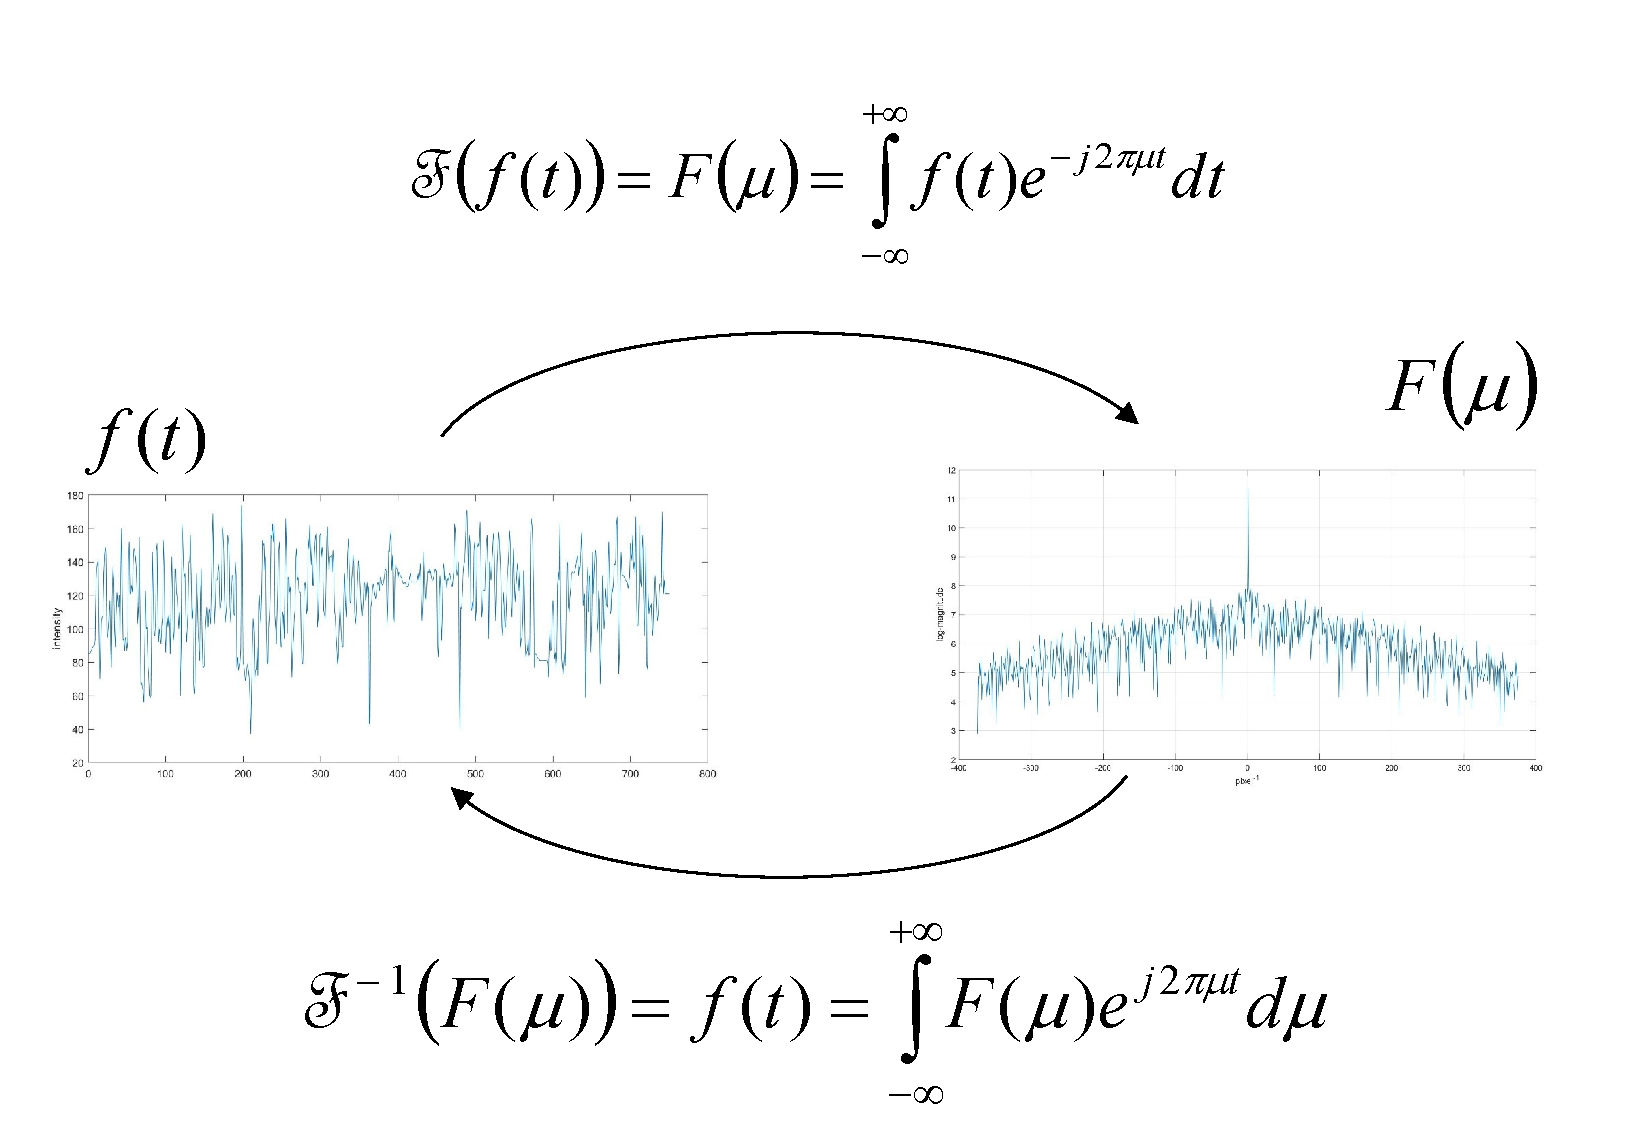
\includegraphics[width=1\textwidth]{img/trasformata_fourier1.pdf}
		\caption{(Anti)Trasformata di Fourier su un segnale $f\left(t\right)$.}
	\end{figure}

	\newpage

	\noindent
	Nel caso in cui il segnale $f\left(t\right)$ non è reale, la trasformata è complessa:
	
	\begin{itemize}
		\item $t$ rappresenta il \textbf{\underline{tempo}} (in secondi), allora $\mu$ rappresenta gli \textbf{Hertz}, cioè $\frac{\text{numero cicli}}{\text{secondi}}$;
		
		\item $t$ rappresenta lo \textbf{\underline{spazio}} (in metri), allora $\mu$ rappresenta la \textbf{frequenza spaziale}, cioè $\frac{\text{numero cicli}}{\text{metri}}$
	\end{itemize}

	\noindent
	Mentre nella serie di Fourier le funzioni rappresentate negli spettri di ampiezza e di fase erano a \dquotes{pettine} (paragrafo~\ref{funzioni a pettine}), in questo caso le funzioni sono solitamente continue, nello spettro di ampiezza, o continue a tratti:
	
	\begin{figure}[!htp]
		\centering
		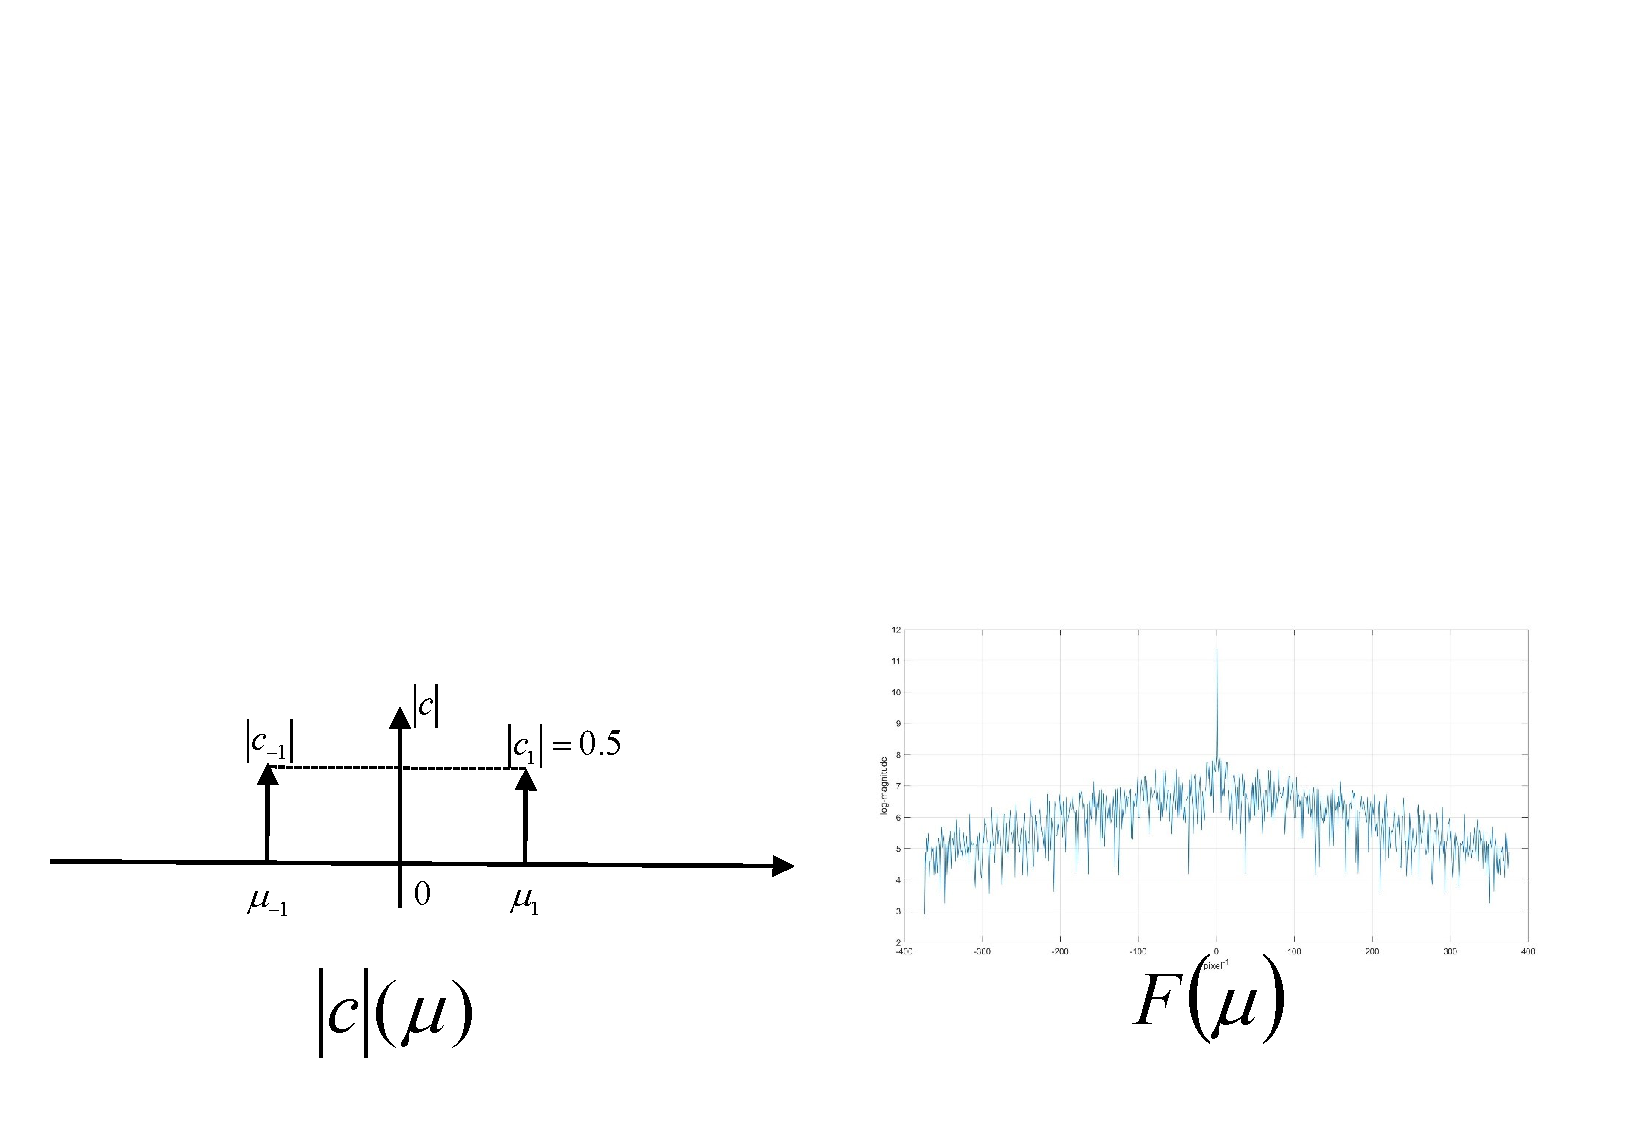
\includegraphics[width=0.9\textwidth]{img/trasformata_fourier2.pdf}
		\caption{Esempio di spettro di ampiezza.}
	\end{figure}
	
	\newpage
	
	\subsubsection{Proprietà della trasformata di Fourier}
	
	\begin{itemize}[label=\ding{42}]
		\item \textcolor{Red3}{\textbf{\underline{Linearità}}}
			\begin{equation*}
				a_{1} f_{1}\left(t\right) + a_{2}f_{2}\left(t\right) \hspace{1em} \xrightarrow{\mathcal{F}} \hspace{1em} a_{1}F_{1}\left(\mu\right) + a_{2}F_{2}\left(\mu\right)
			\end{equation*}
		
		\item \textcolor{Red3}{\textbf{\underline{Scalatura temporale}}}
			\begin{equation*}
				z\left(t\right) = f\left(at\right) \hspace{1em} \xrightarrow{\mathcal{F}} \hspace{1em} Z\left(\mu\right) = \dfrac{1}{a} \: F\left(\dfrac{\mu}{a}\right)
			\end{equation*}
		
		\item \textcolor{Red3}{\textbf{\underline{Dualità}}}
			\begin{gather*}
				f\left(t\right) \hspace{1em} \xrightarrow{\mathcal{F}} \hspace{1em} F\left(\mu\right) \\
				F\left(t\right) \hspace{1em} \xrightarrow{\mathcal{F^{-1}}} \hspace{1em} f\left(-\mu\right)
			\end{gather*}
			N.B. derivando la forma analitica per una trasformata, la sua antitrasformata ne produce un'altra con segno opposto.
			
		\item \textcolor{Red3}{\textbf{\underline{Time shift}}}
			\begin{equation*}
				\begin{matrix}
					\mathcal{F}\left(f\left(t-t_{0}\right)\right) & = & \displaystyle \int_{-\infty}^{+\infty} f\left(t-t_{0}\right) e^{-j 2 \pi \mu t} \: \mathrm{d}t \\
					\\
					& = & \displaystyle \int_{-\infty}^{+\infty} f\left(u\right) e^{-j 2 \pi \mu \left(u + t_{0}\right)} \: \mathrm{d}u \\
					\\
					& = & \displaystyle \int_{-\infty}^{+\infty} f\left(u\right) e^{-j 2 \pi \mu u} e^{-j 2 \pi \mu t_{0}} \: \mathrm{d}u \\
					\\
					& = & \displaystyle e^{-j 2 \pi \mu t_{0}} \: \int_{-\infty}^{+\infty} f\left(u\right) e^{-j 2 \pi \mu u} \: \mathrm{d}u \\
					\\
					& = & F\left(\mu\right) e^{\overbrace{- j 2 \pi \mu t_{0}}^{fase}}
				\end{matrix}
			\end{equation*}
	\end{itemize}

	\newpage
	
	\subsubsection{Trasformata di Fourier di una box}
	
	La trasformata di Fourier di una box (paragrafo~\ref{funzione box e impulso di Dirac}) è la seguente:
	
	\begin{equation*}
		\mathcal{F}\left(f\left(t\right)\right) = \int_{-\infty}^{+\infty} A \Pi \left(\dfrac{t}{w}\right) e^{-j 2 \pi \mu t} \: \mathrm{d}t = F\left(\mu\right)
	\end{equation*}

	\noindent
	Il \textbf{\underline{risultato corrisponde alla funzione}} $\mathrm{sinc}$:
	
	\begin{equation*}
		f\left(\mu\right) = Aw \cdot \mathrm{sinc }\left(\mu w\right)
	\end{equation*}
	
	\noindent
	Dove la funzione $\mathrm{sinc}$ è uguale a:
	
	\begin{equation*}
		\mathrm{sinc} = \dfrac{\sin\left(\pi \mu w\right)}{\pi \mu w}
	\end{equation*}

	\noindent
	Per ripassare la funzione $\mathrm{sinc}$, si rimanda al paragrafo~\ref{funzione sinc}. Tuttavia, si ricorda che la sua forma generale è del tipo:
	
	\begin{equation*}
		\mathrm{sinc} \left(m\right) = \dfrac{\sin \left(\pi m\right)}{\pi m}
	\end{equation*}

	\noindent
	E risultata uguale a:
	
	\begin{itemize}
		\item $\mathrm{sinc}\left(0\right) = 1$
		\item $\mathrm{sinc}\left(m\right) = 0 \hspace{1em} \forall m \in \mathbb{Z}$
	\end{itemize}

	\noindent
	Prima di concludere, si ricorda che:
	
	\begin{itemize}[label=\ding{43}]
		\item All'\textbf{aumentare} della \textbf{larghezza} della box, la funzione $\mathrm{sinc}$ tenderà a \textbf{stringersi};
		
		\item La box è \textbf{limita}, invece la $\mathrm{sinc}$ è \textbf{infinita} a destra e sinistra, anche se il termine al denominatore attenua il valore della funzione comportando un limite a $0$.
			
		\item In sintesi, la TdF di una box è:
			\begin{equation*}
				\Pi\left(\dfrac{t}{w}\right) \hspace{1em} \xrightarrow{\mathcal{F}} \hspace{1em} w \cdot \mathrm{sinc} \left(\mu w\right)
			\end{equation*}
	\end{itemize}

	\begin{figure}[!htp]
		\centering
		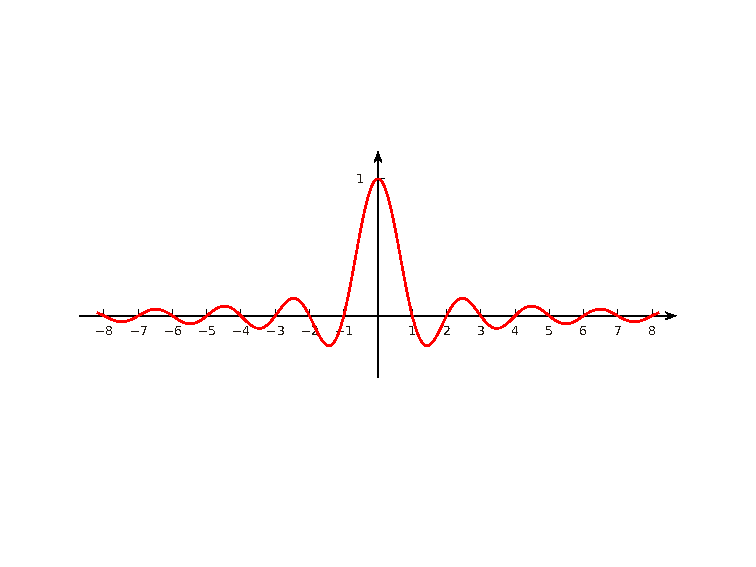
\includegraphics[width=0.8\textwidth]{img/sinc.pdf}
		\caption{Grafico della funzione sinc.}\label{grafico sinc}
	\end{figure}

	\newpage

	\subsubsection[Trasformata di Fourier di un $\mathrm{sinc}$]{Trasformata di Fourier di un $\boldsymbol{\mathrm{sinc}}$}
	
	La trasformata di Fourier di un segnale $\mathrm{sinc}$ (segnale rappresentato in figura~\ref{grafico sinc}) è la seguente:
	
	\begin{equation*}
		\mathcal{F}\left(f\left(t\right)\right) = \int_{-\infty}^{+\infty} \mathrm{sinc}\left(tw\right) e^{-j 2 \pi \mu t} \: \mathrm{d}t = F\left(\mu\right)
	\end{equation*}

	\noindent
	Dato che la TdF di una box è:
	
	\begin{equation*}
		\Pi\left(\dfrac{t}{w}\right) \hspace{1em} \xrightarrow{\mathcal{F}} \hspace{1em} w \cdot \mathrm{sinc} \left(\mu w\right)
	\end{equation*}

	\noindent
	Al contrario, si ottiene la \textbf{\underline{trasformata di Fourier di un $\mathrm{sinc}$}}:
	
	\begin{equation*}
		\mathrm{sinc}\left(tw\right) \hspace{1em} \xrightarrow{\mathcal{F}} \hspace{1em} \dfrac{1}{w} \Pi \left(-\dfrac{\mu}{w}\right) = \dfrac{1}{w} \cdot \Pi \left(\dfrac{\mu}{w}\right)
	\end{equation*}

	\newpage

	\subsubsection{Trasformata di Fourier di un impulso}
	
	La trasformata di Fourier di un impulso\footnote{Definizione di impulso al paragrafo~\ref{funzione box e impulso di Dirac}.} è la seguente:
	
	\begin{equation*}
		\mathcal{F}\left(f\left(t\right)\right) = F\left(\mu\right) = \int_{-\infty}^{+\infty} \delta\left(t\right) e^{-j 2 \pi \mu t} \: \mathrm{d}t
	\end{equation*}

	\noindent
	Il risultato della trasformata di Fourier di un impulso è molto semplice grazie alle sue proprietà. Infatti, il risultato è uguale a:
	
	\begin{equation*}
		\int_{-\infty}^{+\infty} \delta\left(t\right) e^{-j 2 \pi \mu t} \: \mathrm{d}t = \int_{-\infty}^{+\infty} \delta\left(0\right) e^{-j 2 \pi \mu 0} \: \mathrm{d}t = 1
	\end{equation*}

	\noindent
	La proprietà che consente di ottenere il risultato uguale a $1$ è la seguente:
	
	\begin{equation*}
		\delta\left(t\right) =
		\begin{cases}
			\infty  & \text{se } t = 0 \\
			0		& \text{se } t \ne 0
		\end{cases}
		\hspace{2em} \longrightarrow \hspace{2em}
		\int_{-\infty}^{+\infty}\delta\left(t\right)\mathrm{d}t = 1
	\end{equation*}

	\noindent
	\textbf{\underline{N.B. In questo caso è rappresentabile solo lo spettro di ampiezza!}}\newline
	
	\noindent
	Analogamente, con un impulso centrato in $t_{0}$, quindi non nell'origine:
	
	\begin{equation*}
		\mathcal{F}\left(f\left(t\right)\right) = F\left(\mu\right) = \int_{-\infty}^{+\infty} \delta\left(t-t_{0}\right) e^{-j 2 \pi \mu t} \: \mathrm{d}t = e^{-j 2 \pi \mu t_{0}}
	\end{equation*}

	\noindent
	Il risultato è stato ottenuto grazie alla proprietà di setacciamento (definita a pagina~\pageref{setacciamento}). Tuttavia, in questo caso i valori non sono più reali ma complessi.
	
	\newpage
	
	\subsubsection{Trasformata di Fourier di un treno di impulsi}
	
	Data la definizione di treno di impulsi (funzione definita nel paragrafo~\ref{treno_di_impulsi}):
	
	\begin{equation*}
		S_{\Delta T}\left(t\right) = \sum_{n = -\infty}^{+\infty} \delta\left(t - n\Delta T\right) \hspace{1em} n \in \mathbb{Z}
	\end{equation*}

	\noindent
	Si ottiene la sua relativa trasformata di Fourier:
	
	\begin{equation*}
		\mathcal{F}\left(S_{\Delta T}\left(t\right)\right) = \int_{-\infty}^{+\infty} S_{\Delta T}\left(t\right) e^{-j 2 \pi \mu t}\: \mathrm{d}t = F\left(\mu\right)
	\end{equation*}

	\noindent
	Tralasciando i vari calcoli numerici per arrivare al risultato, si può scrivere la trasformata di Fourier in maniera più semplice:
	
	\begin{equation*}
		S_{\Delta T}\left(t\right) \hspace{2em} \xrightarrow{\mathcal{F}} \hspace{2em} \sum_{n = -\infty}^{+\infty} \dfrac{1}{\Delta T} \delta\left(\mu - \dfrac{n}{\Delta T}\right)
	\end{equation*}

	\newpage
	
	\subsubsection{Sintesi}
	
	Qui di seguito si lascia un riassunto rapido delle trasformate di Fourier continue dei segnali più importanti.
	
	\begin{table}[!htbp]
		\centering
		\begin{tabular}{@{} l l c l @{}}
			\toprule
			Segnale & & & Trasformata di Fourier \\
			\midrule
			Box:				& $A\Pi\left(\dfrac{t}{w}\right)$	& $\xrightarrow{\mathcal{F}}$ & $Aw \cdot \mathrm{sinc}\left(\mu w\right)$ \\
			&&&\\
			Sinc:				& $\mathrm{sinc}\left(tw\right)$	& $\xrightarrow{\mathcal{F}}$ & $\dfrac{1}{w}\cdot\Pi \left(-\dfrac{\mu}{w}\right) = \dfrac{1}{w}\cdot \Pi\left(\dfrac{\mu}{w}\right)$ \\
			&&&\\
			Impulso:			& $\delta\left(t\right)$			& $\xrightarrow{\mathcal{F}}$ &
			$\begin{cases}
				1 						& \text{se valori reali}\\
				e^{-j 2 \pi \mu t_{0}}	& \text{se valori complessi}
			\end{cases}$ \\
			&&&\\
			Treno di impulsi:	& $S_{\Delta T}\left(t\right)$ 		& $\xrightarrow{\mathcal{F}}$ & $\displaystyle\sum_{n = -\infty}^{+\infty} \dfrac{1}{\Delta T} \cdot \delta \left(\mu - \dfrac{n}{\Delta T}\right)$ \\
			\bottomrule
		\end{tabular}
		\caption{Trasformate di Fourier continue.}
	\end{table}

	\newpage
	
	\subsection{Trasformata di Fourier a tempo discreto}\label{trasformata di fourier a tempo discreto}
	
	\subsubsection{Campionamento}
	
	Sia $f\left(t\right)$ un segnale reale continuo definito $f : \left] -\infty, + \infty \right[ \in \mathbb{R} \rightarrow \mathbb{R}$ (attenzione al dominion non limitato), anche non periodico:
	
	\begin{figure}[!htp]
		\centering
		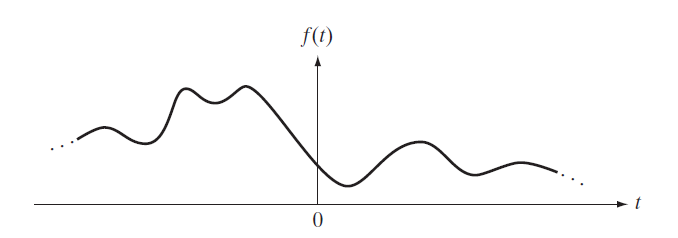
\includegraphics[width=0.65\textwidth]{img/campionamento_1.png}
	\end{figure}

	\noindent
	Questo tipo di segnale, per essere elaborato al computer deve essere \textbf{campionato} ad intervalli discreti. Per farlo, si prenda in considerazione il treno di impulsi:
	
	\begin{equation*}
		S_{\Delta T} \left(t\right) = \sum_{n = -\infty}^{+\infty} \delta\left(t - n\Delta T\right)
	\end{equation*}

	\noindent
	Con periodo $\Delta T$, ossia con \textbf{frequenza di campionamento} pari a: $\mu_{S} = \dfrac{1}{\Delta T}$

	\begin{figure}[!htp]
		\centering
		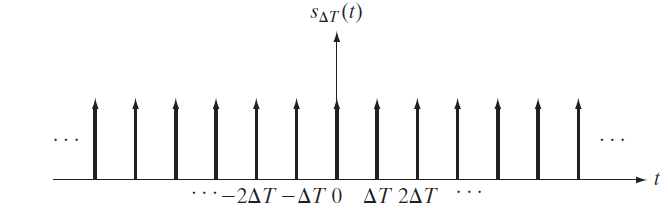
\includegraphics[width=0.65\textwidth]{img/campionamento_2.png}
	\end{figure}

	\noindent
	Si assuma che il treno di impulsi sia un \textbf{segnale discreto}. Matematicamente parlando, \textbf{campionare un segnale \underline{significa} moltiplicarlo per un treno di impulsi}:
	
	\begin{equation*}
		\tilde{f}\left(t\right) = f\left(t\right) \cdot S_{\Delta T}\left(t\right) = f\left(t\right) \cdot \sum_{n = -\infty}^{+\infty} \delta\left(t - n \Delta T\right)
	\end{equation*}

	\begin{figure}[!htp]
		\centering
		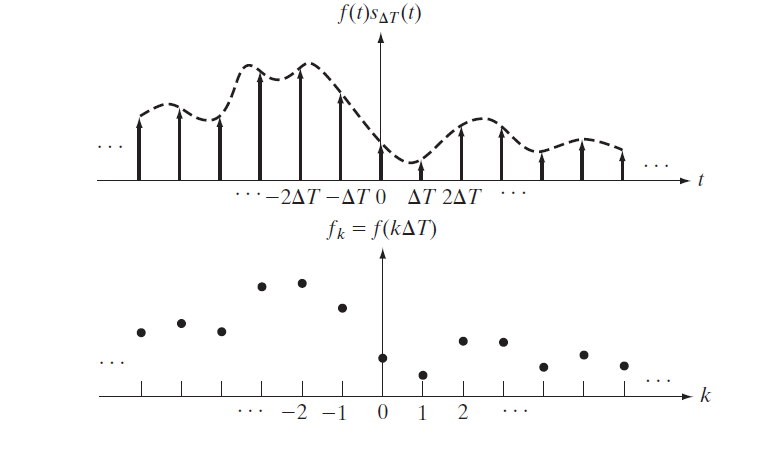
\includegraphics[width=0.65\textwidth]{img/campionamento_3.png}
	\end{figure}
	
	\newpage
	
	\subsubsection{Trasformata di Fourier a tempo discreto}
	
	Sia $F\left(\mu\right)$ la trasformata di Fourier di un segnale $f\left(t\right): \mathbb{R} \rightarrow \mathbb{R}$. Si considera $\tilde{f}\left(t\right)$ e si calcola la trasformata di Fourier $\tilde{F}\left(\mu\right)$ (entrambi sono a tempo discreto). Grazie alla convoluzione si ottiene:
	
	\begin{equation*}
		\tilde{F}\left(\mu\right) = \mathcal{F}\left\{\tilde{f}\left(t\right)\right\} = F\left(\mu\right) * S_{\Delta T}\left(\mu\right)
	\end{equation*}

	\noindent
	Si ricorda che:
	
	\begin{equation*}
		S_{\Delta T} \left(\mu\right) = \dfrac{1}{\Delta T} \sum_{n = -\infty}^{+\infty}\delta\left(\mu - \dfrac{n}{\Delta T}\right)
	\end{equation*}	

	\noindent
	E risolvendo la convoluzione, si ottiene che la \textcolor{Red3}{\textbf{\underline{trasformata di Fourier a tempo}}} \textcolor{Red3}{\textbf{\underline{discreto}}} corrisponde a:
	
	\begin{equation*}
		F\left(\mu\right) * S_{\Delta T}\left(\mu\right) = \int_{-\infty}^{+\infty} F\left(\tau\right) \cdot S_{\Delta T} \left(\mu - \tau\right) \: \mathrm{d}\tau = \dfrac{1}{\Delta T} \sum_{n = -\infty}^{+\infty} F \left(\mu - \dfrac{n}{\Delta T}\right)
	\end{equation*}

	\noindent
	Analizzando la formula si evidenziano alcuni termini:
	
	\begin{itemize}
		\item $F\left(\mu\right)$ è la trasformata di Fourier della funzione originale $f\left(t\right)$;
		
		\item $F\left(\mu - \dfrac{n}{\Delta T}\right)$ è la trasformata di Fourier della funzione originale $f\left(t\right)$ shiftato a destra di una quantità pari a $\dfrac{n}{\Delta T}$;
		
		\item $\dfrac{1}{\Delta T} \sum_{n = -\infty}^{+\infty} F \left(\mu - \dfrac{n}{\Delta T}\right)$ sono infinite copie dello spettro $F\left(\mu\right)$, ripetute ovviamente ogni $\dfrac{1}{\Delta T}$. \newline
		Inoltre, è un \textbf{segnale periodico} (nelle frequenze) di periodo $\dfrac{1}{\Delta T}$, ovvero si ripete ogni $\dfrac{1}{\Delta T}$ Hz.\newline
		La sua scalatura nell'ampiezza è pari a $\dfrac{1}{\Delta T}$ e rappresenta la T.d.F. a tempo discreto.
	\end{itemize}

	\newpage
	
	\subsubsection{Teorema del campionamento}
	
	Un \textbf{\underline{segnale reale continuo}} $f\left(t\right)$, limitato in banda, può essere \textbf{\underline{ricostruito}} \textbf{\underline{senza errori completamente dai suoi campioni}} se essi sono acquisiti con un tempo di campionamento $\Delta T$ tale per cui:
	
	\begin{equation*}
		\dfrac{1}{\Delta T} = \mu_{S} \ge 2 \mu_{\text{max}}
	\end{equation*}

	\noindent
	Ovvero se nel tempo si adotta una frequenza di campionamento $\dfrac{1}{\Delta T}$ almeno doppia rispetto alla frequenza massima del segnale $\mu_{\text{max}}$.\newline
	In altre parole, il teorema del campionamento afferma che tutte le proprietà di un segnale possono essere espresse usando dei campioni.\newline
	
	\noindent
	\textbf{\underline{Attenzione!}} L'espressione $\dfrac{1}{\Delta T}$ viene chiamata \textbf{\emph{frequenza di Nyquist}} e per frequenze minori si crea aliasing, fenomeno che impedisce la ricostruzione senza errori.
	
	\subsubsection{Considerazioni}
	
	Dal \textbf{\underline{punto di vista teorico}} la trasformata di Fourier a tempo discreto consente di ricostruire il segnale. Tuttavia, è impossibile implementarla in un computer poiché tende, come limiti, all'infinito e ci vorrebbe un numero infinito di campioni e di segnali di tipo $\mathrm{sinc}$.
	
	\newpage
	
	\subsection{Trasformata di Fourier discreta}\label{trasformata di fourier discreta}
	
	La trasformata di Fourier di un segnale reale continuo $f\left(t\right)$ di dominio illimitato e non periodico, campionato nel tempo con periodo di campionamento $\Delta T$, è una funzione continua, periodica (di periodo $\dfrac{1}{\Delta T}$) anch'essa di dominio illimitato:
	
	\begin{equation*}
		\tilde{f}\left(t\right) = f\left(t\right) \cdot \sum_{n = -\infty}^{+\infty}\delta\left(t - n\Delta T\right) \: \textcolor{Red3}{\overset{\mathcal{F}}{\longrightarrow}} \: \tilde{F}\left(\mu\right) = \dfrac{1}{\Delta T} \sum_{n = -\infty}^{+\infty} F\left(\mu - \dfrac{n}{\Delta T}\right)
	\end{equation*}

	\noindent
	Il \textbf{problema} di questa formulazione è data l'espressione analitica dello spettro, la quale suppone che si è a \textbf{conoscenza della T.d.F.} teorica $F$ \textbf{del segnale di partenza}. Questo, spesso, è molto difficile.\newline
	
	\noindent
	Si ricava dunque una \emph{forma più semplice} da manipolare. Essa consente di \textbf{costruire una rappresentazione spettrale a partire dai campioni della funzione originale} $f\left(t\right)$:
	
	\begin{equation*}
		\tilde{F}\left(\mu\right) = \sum_{n = -\infty}^{+\infty} f_{n} \: e^{-j 2 \pi \mu n \Delta T}
	\end{equation*}
	
	\noindent
	Al contrario, la prima formulazione era più chiara per comprendere il fatto che la T.d.F. di una funzione campionata genera delle repliche dello spettro originale $F\left(\mu\right)$.\newline
	
	\noindent
	L'equazione alternativa deve essere modificata, eseguendo un campionamento per il dominio spettrale, per poterla implementare su un computer. Per farlo, si prende in considerazione solo l'intervallo frequenziale da $0$ a $\dfrac{1}{\Delta T} = \mu_{S}$.
	
	\begin{figure}[!htp]
		\centering
		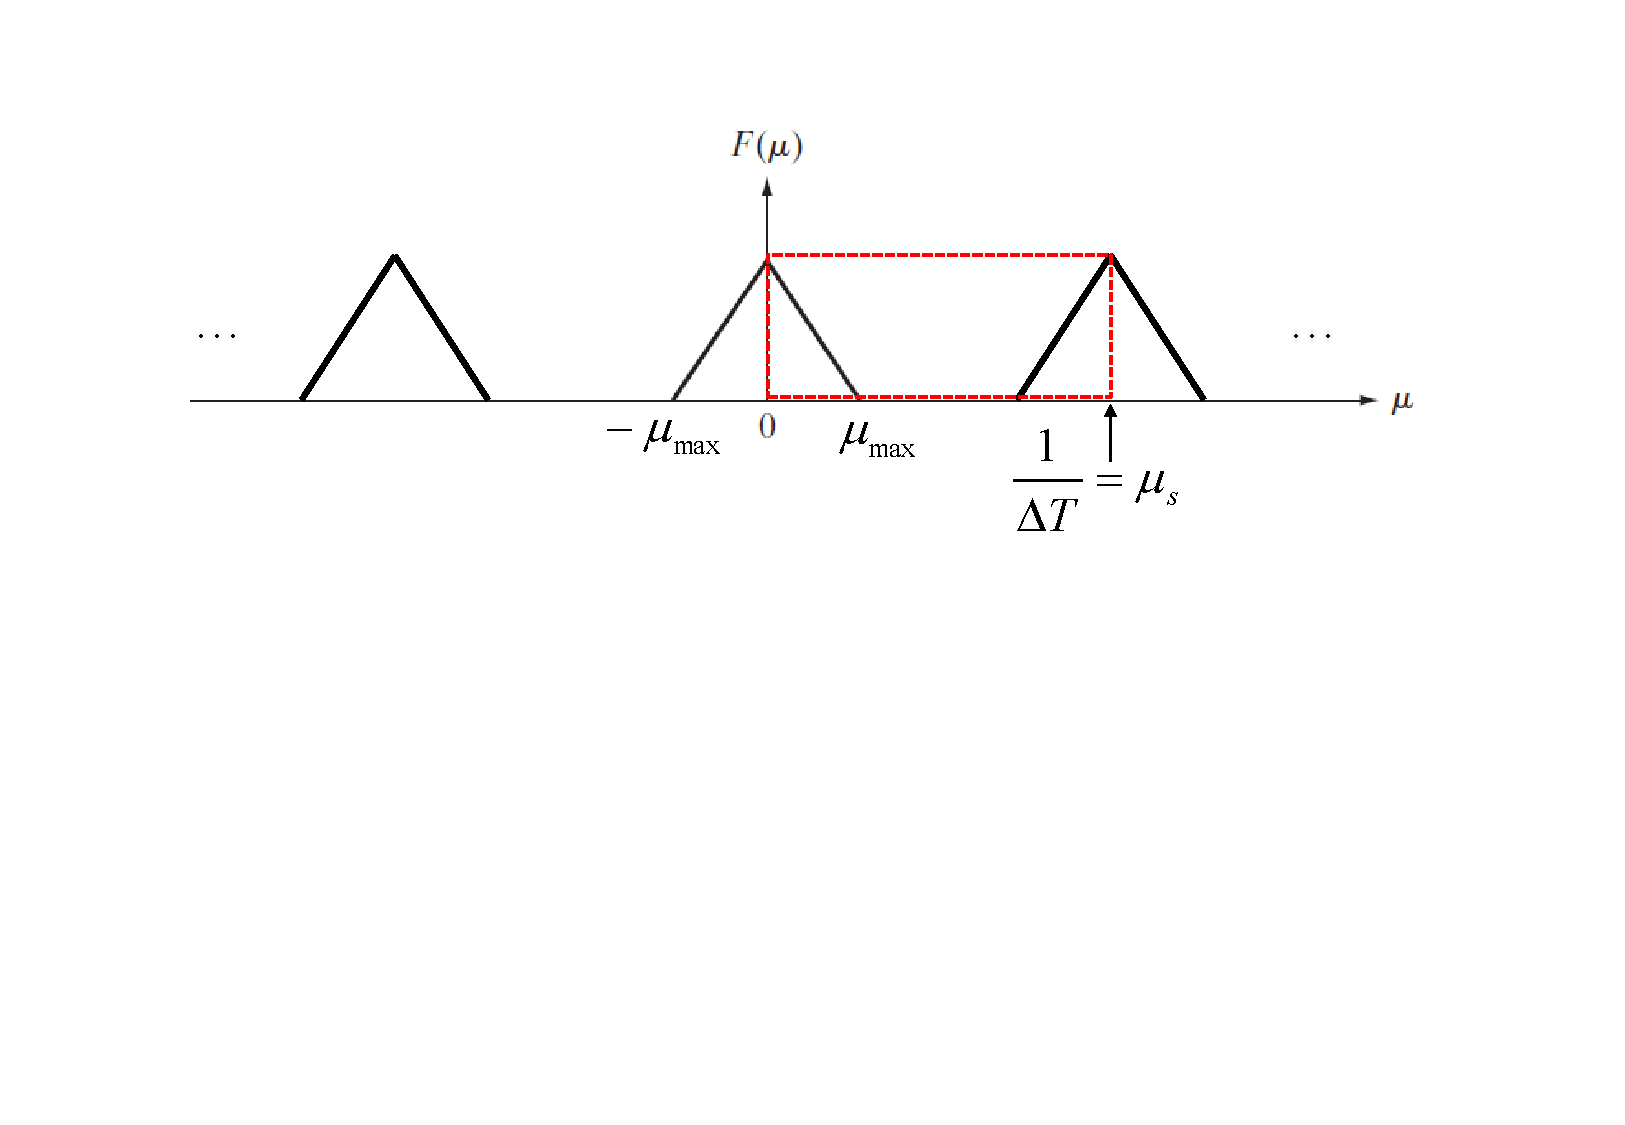
\includegraphics[width=0.7\textwidth]{img/trasformata_fourier_discreta1.pdf}
	\end{figure}

	\noindent
	Inoltre, si prendono in considerazione $M$ campioni tramite l'operazione di campionamento.
	
	\begin{figure}[!htp]
		\centering
		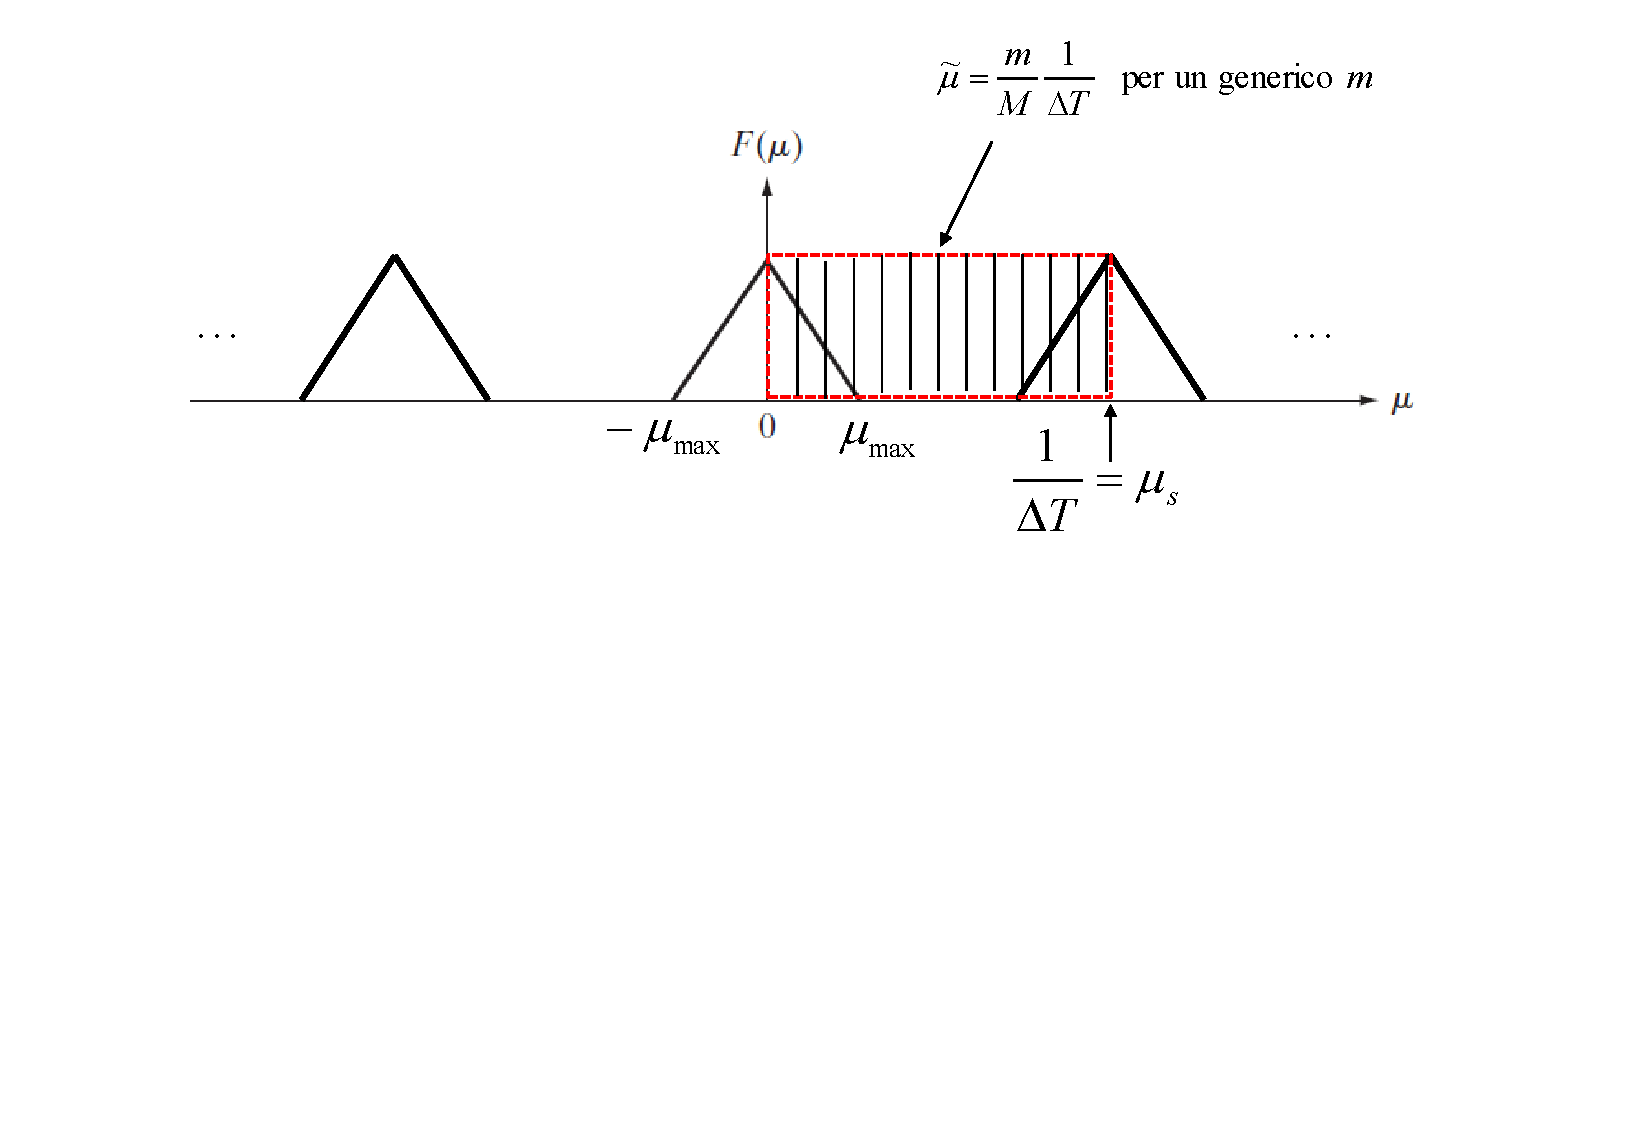
\includegraphics[width=0.7\textwidth]{img/trasformata_fourier_discreta2.pdf}
	\end{figure}

	\newpage

	\noindent
	In cui:
	
	\begin{equation*}
		\tilde{\mu} = \dfrac{m}{M} \cdot \dfrac{1}{\Delta T} \hspace{2em} \text{con } m = 0, ..., M-1 \text{ e dove } \dfrac{m}{M} \in \left[0,1 - \dfrac{1}{M}\right]
	\end{equation*}

	\noindent
	La $m$ indica il \textbf{range di variazione} degli indici dei campioni frequenziali. Calcolando la trasformata di Fourier a tempo discreto sui campioni $M$, si giunge alla \textcolor{Red3}{\textbf{\underline{forma finale della trasformata di Fourier discreta}}}:
	
	\begin{equation*}
		\tilde{F}\left(\tilde{\mu}\right) = \tilde{F}\left(\dfrac{m}{M} \cdot \dfrac{1}{\Delta T}\right) = \sum_{n = 0}^{M - 1} f_{n} e^{-j 2 \pi \frac{m}{M} n} \hspace{2em} \text{con } m = 0, ..., M - 1
	\end{equation*}

	\noindent
	La \textcolor{Red3}{\textbf{\underline{trasformata di Fourier discreta inversa}}}, ovvero l'antitrasformata:
	
	\begin{equation*}
		\tilde{f}\left(n \Delta T\right) = f\left(n \Delta T\right) = f_{n} = \dfrac{1}{M} \sum_{m = 0}^{M - 1} F_{m} e^{j 2 \pi \frac{m}{M} n}
	\end{equation*}

	\newpage
	
	\subsection{Riassunto Trasformate}
	
	Qui di seguito vengono rappresentate le trasformate più importanti.
	
	\begin{table}[!htbp]
		\centering
		\begin{tabular}{@{} l l c l @{}}
			\toprule
			%Segnale & & & Trasformata di Fourier \\
			Funzione & & & Serie di Fourier \\
			\midrule
			&&& \\
			Funzione di sintesi: & $f(t)$ && $\sum_{n = -\infty}^{+\infty} c_{n} \underbrace{e^{j \frac{2\pi n}{T}t}}_{\text{fasore}} \hspace{2em} n\in\mathbb{Z}$ \\
			&&& \\
			Funzione di analisi: & $c_{n} \in \mathbb{C}$ && $\dfrac{1}{T} \int_{-\frac{T}{2}}^{+\frac{T}{2}} f\left(t\right) \underbrace{e^{-j \frac{2\pi n}{T}t}}_{\text{fasore}} \mathrm{d}t \hspace{2em} n \in \mathbb{Z}$ \\
			&&& \\
			\toprule
			Segnale  & & & Trasformata di Fourier continua \\
			\midrule
			Box:				& $A\Pi\left(\dfrac{t}{w}\right)$	& $\xrightarrow{\mathcal{F}}$ & $Aw \cdot \mathrm{sinc}\left(\mu w\right)$ \\
			&&&\\
			Sinc:				& $\mathrm{sinc}\left(tw\right)$	& $\xrightarrow{\mathcal{F}}$ & $\dfrac{1}{w}\cdot\Pi \left(-\dfrac{\mu}{w}\right) = \dfrac{1}{w}\cdot \Pi\left(\dfrac{\mu}{w}\right)$ \\
			&&&\\
			Impulso:			& $\delta\left(t\right)$			& $\xrightarrow{\mathcal{F}}$ &
			$\begin{cases}
				1 						& \text{se valori reali}\\
				e^{-j 2 \pi \mu t_{0}}	& \text{se valori complessi}
			\end{cases}$ \\
			&&& \\
			Treno di impulsi:	& $S_{\Delta T}\left(t\right)$ 		& $\xrightarrow{\mathcal{F}}$ & $\displaystyle\sum_{n = -\infty}^{+\infty} \dfrac{1}{\Delta T} \cdot \delta \left(\mu - \dfrac{n}{\Delta T}\right)$ \\
			&&& \\
			\toprule
			Funzione & & & Trasformata di Fourier a tempo discreto \\
			\midrule
			&&& \\
			$F\left(\mu\right) * S_{\Delta T}\left(\mu\right)$ & & & $\dfrac{1}{\Delta T} \sum_{n = -\infty}^{+\infty} F \left(\mu - \dfrac{n}{\Delta T}\right)$ \\
			&&& \\
			\toprule
			Funzione & & & Trasformata di Fourier discreta \\
			\midrule
			&&& \\
			$\tilde{F}\left(\tilde{\mu}\right)$ &&& $\tilde{F}\left(\dfrac{m}{M} \cdot \dfrac{1}{\Delta T}\right) = \sum_{n = 0}^{M - 1} f_{n} e^{-j 2 \pi \frac{m}{M} n}$ \\
			&&& \\
			&&& $m = 0, ..., M - 1$ \\
			&&& \\
			\toprule
			Funzione & & & Trasformata di Fourier discreta inversa \\
			\midrule
			&&& \\
			$\tilde{f}\left(n \Delta T\right) = f\left(n \Delta T\right) = f_{n}$ &&& $\dfrac{1}{M} \sum_{m = 0}^{M - 1} F_{m} e^{j 2 \pi \frac{m}{M} n}$ \\
			&&& \\
			\bottomrule
		\end{tabular}
		\caption{Trasformate di Fourier.}
	\end{table}
	
	\newpage
	
	\subsection{Domanda da \textcolor{Red3}{esame}}
	
	All'esame è possibile che sia richiesto come domanda: \dquotes{quali sono le trasformate di Fourier studiate durante il corso?}
	
	La risposta, anche se banale, è la seguente: le trasformate di Fourier studiate durante il corso sono $4$:
	
	\begin{enumerate}[label=\Roman*.]
		\item Serie di Fourier (paragrafo~\ref{serie di fourier})
		\item Trasformata di Fourier continua (paragrafo~\ref{trasformata di fouerier continua})
		\item Trasformata di Fourier a tempo discreto (paragrafo~\ref{trasformata di fourier a tempo discreto})
		\item Trasformata di Fourier discreta (paragrafo~\ref{trasformata di fourier discreta})
	\end{enumerate}

	\newpage
	
	\section{Elaborazione di immagini - Dominio spaziale}
	
	L'\textcolor{Red3}{\textbf{\underline{elaborazione delle immagini}}} consiste nel prendere come input un'immagine (segnale) e restituirne un'altra (sempre segnale) come output.\newline
	
	\noindent
	Il \textcolor{Red3}{\textbf{\underline{rinforzo (\emph{enhancement}) di immagini}}} è un tipo di elaborazione delle immagini. Il suo \textbf{obbiettivo} è elaborare un'immagine in modo che il risultato sia più adatto alle esigenze soggettive dell'utente. La definizione è \emph{problem-oriented} poiché, per esempio, per visualizzare lo spettro di ampiezza di un'immagine, è necessario eseguire un'operazione di rinforzo (\emph{log-transformation}); oppure, per migliorare la visibilità dei dettagli di un'immagine, si effettua un'altra operazione di rinforzo (\emph{sharpening}).\newline
	
	\noindent
	La \textcolor{Red3}{\textbf{\underline{qualità di un'immagine}}} è la combinazione pesata di tutti gli attributi significativi di un'immagine. Infatti, \emph{non} esiste una ricetta univoca per determinare quando un'immagine sia di qualità poiché è un'opinione soggettiva. Tuttavia, è più facile dire quando un'immagine \emph{non} è di qualità. In genere, un'\textcolor{Red3}{\textbf{\underline{immagine \emph{non} è di qualità}}} quando non viene interpretata facilmente da un operatore umano.\newline
	
	\noindent
	A differenza del rinforzo, il \textcolor{Red3}{\textbf{\underline{restauro (\emph{restoration})}}} è un processo di ricostruzione dell'immagine a partire da un modello di degradazione noto.
	
	\newpage
	
	\subsection{Strumento per l'elaborazione: istogramma}
	
	I pixel di un'immagine sono una \dquotes{popolazione} sulla quale è possibile calcolare tutte le quantità statistiche descrittive che vengono usate normalmente come media, mediana, varianza, deviazione standard, quartili, percentili, etc. Uno \textbf{strumento fondamentale} per l'elaborazione delle immagini è l'\textcolor{Red3}{\textbf{\underline{istogramma}}}, il quale può essere visto come una funzione continua o discreta.\newline
	
	\noindent
	Infatti, per ogni livello di grigio (in un'immagine solo a livelli di grigi) vengono riportati il numero di pixel. Per un'immagine $I\left[M,N\right]$ si identifica con $M,N$ il \textbf{numero di pixel righe per colonne} e con la funzione $H\left(r\right)$ il \textbf{numero di pixel di valore} $r$, quest'ultimo è definito nell'intervallo $0 \le r \le L-1$ con $r,L \in \mathbb{N}$ dove $L$ indica i livelli di grigio. Inoltre:
	
	\begin{equation*}
		\sum_{r = 0}^{L - 1} H\left(r\right) = M \cdot N
	\end{equation*}

	\noindent
	Grazie all'istogramma, è possibile comprendere immediatamente le caratteristiche dell'immagine (come in figura).
	
	\begin{figure}[!htp]
		\centering
		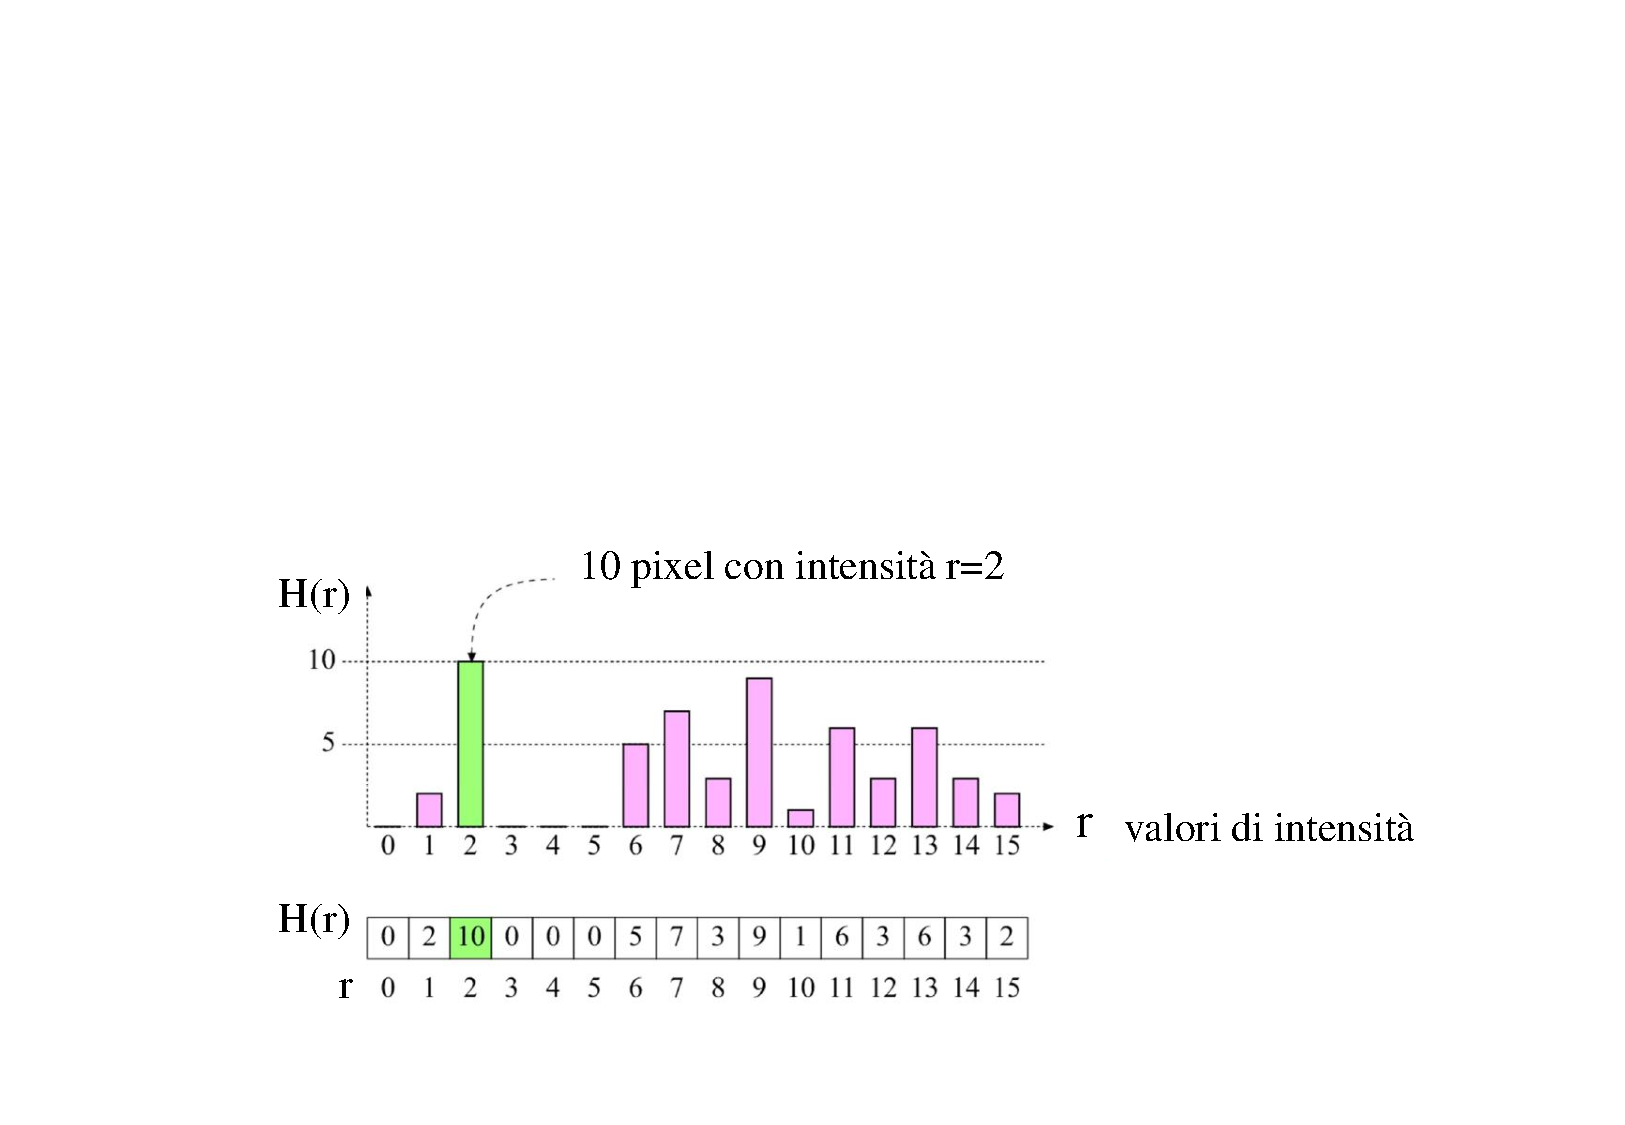
\includegraphics[width=0.8\textwidth]{img/istogramma.pdf}
		\caption{Esempio di istogramma.}
	\end{figure}

	\noindent
	Un istogramma può essere anche visto come una distribuzione di probabilità:
	
	\begin{equation*}
		p_{h}\left(r\right) = \dfrac{H\left(r\right)}{M \cdot N} \hspace{2.5em} \sum_{r} p_{h}\left(r\right) = 1
	\end{equation*}

	\noindent
	Uno \textcolor{Red3}{\textbf{\underline{svantaggio}}} di questo strumento è che immagini diverse potrebbero avere istogrammi simili, questo perché l'istogramma non tiene conto della distribuzione spaziale dei pixel. Dunque, \textbf{utilizzando solo questo metodo è impossibile ricostruire un'immagine}.\newline
	
	\noindent
	Al contrario, un \textcolor{Green4}{\textbf{\underline{vantaggio}}} dell'istogramma è la possibilità di identificare facilmente il \textcolor{Red3}{\textbf{contrasto}}: rapporto o differenza tra il valore più alto (punto più luminoso) e il valore più basso (punto più scuro) della luminosità (che corrisponde al livello di grigio per le immagini a livello di grigio).\newline
	Un'immagine viene definita:
	
	\begin{itemize}
		\item Valori più alti sulla destra:
		\begin{itemize}
			\item \textbf{chiara}, caratteristica dell'immagine;
			\item \textbf{sovraesposta}, caratteristica di come è stata acquisita l'immagine.
		\end{itemize}
	
		\item Valori più alti sulla sinistra:
		\begin{itemize}
			\item \textbf{scura}, caratteristica dell'immagine;
			\item \textbf{sottoesposta}, caratteristica di come è stata acquisita l'immagine.
		\end{itemize}
	\end{itemize}

	\newpage
	
	\subsection{Domini}
	
	L'elaborazione delle immagini può avvenire nel \textbf{dominio spaziale} o nel \textbf{dominio frequenziale} (dopo aver applicato la T.d.F. discreta 2D). Nel \textcolor{Red3}{\textbf{\underline{dominio spaziale}}}, l'elaborazione delle immagine può essere espressa come:
	
	\begin{equation*}
		g\left(x,y\right) = T\left[f\left(x,y\right)\right]
	\end{equation*}

	\noindent
	In cui:
	
	\begin{itemize}[label=-]
		\item $f$ è l'immagine di ingresso (input) da elaborare;
		\item $g$ è l'immagine d'uscita (output) elaborata;
		\item $T$ è un operatore su $f$ definito in un intorno di $\left(x,y\right)$.
	\end{itemize}

	\noindent
	L'\textcolor{Red3}{\textbf{\underline{operatore}}} definito in un intorno di $\left(x,y\right)$ può essere di tre tipi:
	
	\begin{itemize}
		\item \textbf{Puntuale:} $\left[f\left(x,y\right)\right] = f\left(x,y\right)$, l'intorno coincide con il pixel stesso;
		
		\item \textbf{Locale:} $\left[f\left(x,y\right)\right]$ rappresenta una regione, per esempio quadrata, attorno al pixel di locazione $\left(x,y\right)$;
		
		\item \textbf{Globale:} $\left[f\left(x,y\right)\right]$ rappresenta l'intera immagine $f$.
	\end{itemize}

	\newpage
	
	\subsection{Operazioni puntuali}
	
	Si dice \textcolor{Red3}{\textbf{\underline{operatore puntuale}}}, un operatore che ha preso in input il valore di un pixel e ne restituisce uno cambiato, il quale dipende esclusivamente dal valore del pixel in ingresso.\newline
	
	\noindent
	L'\textbf{\underline{obbiettivo}} è quello di variare il contrasto. Infatti, eseguendo questa operazione, si evidenziano le differenze strutturali dell'oggetto rappresentato. Per farlo, basta cambiare il valore di un pixel per renderlo più scuro o più chiaro.\newline
	
	\noindent
	Un operatore puntuale può essere rappresentato tramite una \textbf{\underline{funzione}} che prende in input un valore $r$ e lo modifica in un valore $s = T\left(r\right)$ con $s,r$ appartenenti allo stesso campo di definizione (esempio tra 0 e 255). Più in generale viene definita come:
	
	\begin{equation*}
		T: \left[0, L - 1\right] \subset \mathbb{R} \longrightarrow \left[0, L - 1\right] \subset \mathbb{R}
	\end{equation*}

	\noindent
	Dato che un operatore puntuale dipende solo dal singolo valore del pixel, esso è dunque descritto da una tabella di questo tipo:
	
	\begin{center}
		\begin{tabular}{|c|c|c|c|c|c|c|c|c|}
			\hline
			&&&&&&&& \\
			r & 0 & 1 & 2 & 3 & 4 & 5 & 6 & $\cdots$ \\
			&&&&&&&& \\
			\hline
			&&&&&&&& \\
			s & $T\left(0\right)$ & $T\left(1\right)$ & $T\left(2\right)$ & $T\left(3\right)$ & $T\left(4\right)$ & $T\left(5\right)$ & $T\left(6\right)$ & $\cdots$ \\
			&&&&&&&& \\
			\hline
		\end{tabular}
	\end{center}

	\newpage
	
	\subsubsection{Identità}
	
	È l'operazione più semplice e non fa nulla:
	
	\begin{equation*}
		s = r
	\end{equation*}

	\subsubsection{Negativo}
	
	Rende l'immagine più scura:
	
	\begin{equation*}
		s = L - 1 - r
	\end{equation*}

	\noindent
	Nel caso dei livelli di grigio:
	
	\begin{equation*}
		s = 255 - r
	\end{equation*}

	\noindent
	Viene \textbf{utilizzata} quando si hanno dettagli grigi immersi in zone nere che si vogliono evidenziare.

	\subsubsection{Clamping}
	
	Limita l'intensità ad un range definito $\left[a,b\right]$:
	
	\begin{equation*}
		T\left(r\right) = \begin{cases}
			a & \text{se } r < a \\
			r & \text{se } a \le r \le b \\
			b & \text{se } r > b \\
		\end{cases}
	\end{equation*}

	\noindent
	Viene \textbf{utilizzata} nel caso in cui ci siano dei pixel di rumore molto chiari o molto scuri che \emph{mascherano} l'immagine. Quindi, si pensi per esempio ad un'immagine con dei puntini bianchi al quale si applica il \emph{clamping} per rimuoverli.
	
	\subsubsection{Stretching/Shrinking}
	
	Stira/comprime le intensità di un range $\left[r_{\min}, r_{\max}\right]$ ad un range definito $\left[a,b\right]$:
	
	\begin{equation*}
		s = \left[\dfrac{r - r_{\min}}{r_{\max} - r_{\min}}\right] \left[b - a\right] + a
	\end{equation*}

	\noindent
	In cui:
	
	\begin{itemize}
		\item $r_{\min / \max}$ sono il più piccolo/grande livello di grigio del range che si vuole trattare;
		\item $a,b$ sono il minimo e il massimo \dquotes{stretchati}.
	\end{itemize}

	\noindent
	\textbf{Nota bene:} l'operazione è seguita da \emph{rounging} (arrotondamento) nel caso di dominio di valori nei naturali (come in 0-255). Inoltre, lo \textbf{stretching \underline{non} risolve il problema del rumore impulsivo (puntini neri o bianchi)}, neanche se mascherato con il clamping.
	
	\newpage
	
	\subsubsection{Trasformazione logaritmica}\label{trasformazione logaritmica}
	
	La forma generale è:
	
	\begin{equation*}
		s = c \cdot \log\left(1 + r\right) \hspace{2em} r \in \left[0, L - 1\right]
	\end{equation*}

	\noindent
	Con $c$ che rappresenta la \textbf{costante di normalizzazione}:
	
	\begin{equation*}
		c = \dfrac{L - 1}{\log\left(L\right)}
	\end{equation*}
	
	\noindent
	La quale assicura la mappatura in $\left[0, L - 1\right]$. Inoltre, l'aggiunta di $1$ permette di evitare il calcolo di quantità $\in\left[0,1\right[$ che generano valori minori di zero ed in particolare il calcolo di $\log\left(0\right) = -\infty$.\newline
	
	\noindent
	Viene \textbf{utilizzata} quando si vuole mappare fasce strette di valori dell'immagine originale in fasce più ampie, aumentandone così il range del contrasto, rendendo inoltre l'interpretazione umana più informativa.
	
	\subsubsection{Trasformazione esponenziale}
	
	Al contrario della trasformazione logaritmica, la trasformazione esponenziale consente di aumentare il range di una fascia determinata di livelli di grigi chiari:
	
	\begin{equation*}
		s = \left(e^{r}\right)^{\frac{1}{c}} - 1 \hspace{2em} r \in \left[0, L - 1\right]
	\end{equation*}

	\noindent
	Con la \textbf{costante di normalizzazione}:
	
	\begin{equation*}
		c = \dfrac{L - 1}{\log\left(L\right)}
	\end{equation*}

	\newpage

	\subsubsection{Trasformazione di potenza}
	
	La trasformazione di potenza può essere espressa come:
	
	\begin{equation*}
		s = cr^{\gamma} \hspace{2em} c,\gamma > 0 \in \mathbb{R}
	\end{equation*}

	\noindent
	La costante $c$ è scelta \textbf{in dipendenza da} $\gamma$ in modo da normalizzare i valori di $s$ nell'intervallo $\left[0,255\right]$.
	
	\begin{itemize}[label=-]
		\item $\gamma < 1$, la trasformazione ha effetti analoghi alla trasformazione logaritmica (\ref{trasformazione logaritmica}), cioè espansione della dinamica per bassi valori di $r$, mentre compressione della dinamica per alti valori di $r$;
		
		\item $\gamma > 1$, la trasformazione ha effetti opposti ai valori negativi di gamma.
	\end{itemize}

	\noindent
	Nella pratica, il termine di normalizzazione $c$ è complicato da definire analiticamente, quindi si preferiscono due versioni di $s$:
	
	\begin{itemize}
		\item \textbf{Non normalizzata:} $\tilde{s} = r^{\gamma}$;
		
		\item \textbf{Normalizzata} $s = cr^{\gamma}$
	\end{itemize}

	\noindent
	Per passare dalla versione \textbf{non normalizzata alla versione normalizzata} si esegue lo \emph{stretching}:
	
	\begin{equation*}
		s = \left[\dfrac{\tilde{s} - \tilde{s}_{\min}}{\tilde{s}_{\max}} - \tilde{s}_{\min}\right] \left[\max-\min\right]
	\end{equation*}

	\noindent
	Dove $\tilde{s}_{\min / \max}$ sono il più piccolo/grande livello di grigio e $\max$ e $\min$ sono il massimo e il minimo livello di grigio possibile (255, 0).
	
	\subsubsection{Binarizzazione}
	
	Produce un'immagine che ha solo due livelli: nero e bianco. Si \textbf{ottiene} scegliendo una soglia $T$, si imposta a colore nero tutti i pixel il cui valore è minore a $T$ e si imposta a colore bianco tutti gli altri.\newline
	
	\noindent
	Si \textbf{utilizza} la binarizzazione per discriminare un oggetto dalla scena.
	
	\begin{figure}[!htp]
		\centering
		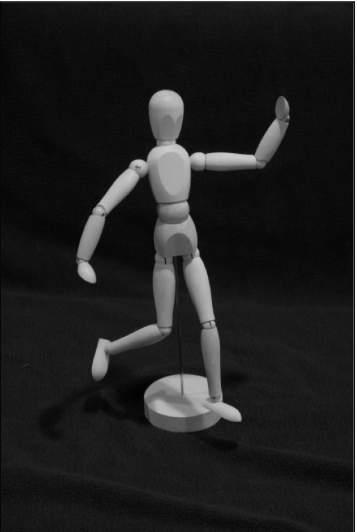
\includegraphics[width=0.2\textwidth]{img/binarizzazione1.png}
		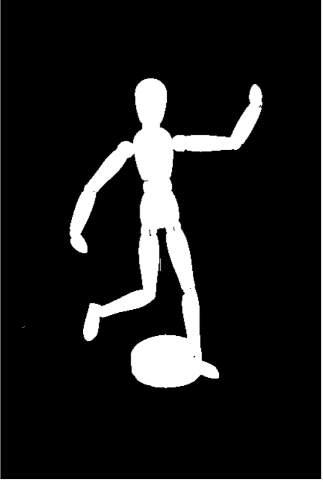
\includegraphics[width=0.2\textwidth]{img/binarizzazione2.png}
	\end{figure}

	\noindent
	Solitamente il suo utilizzo è prevalente nell'ambito delle immagini biomedicali e di videosorveglianza. La difficoltà maggiore di questa tecnica è il saper scegliere la soglia $T$ più ragionevole.
	
	\subsubsection{Binarizzazione attraverso il metodo di Otsu}
	
	Questo metodo assume che ci siano due regioni da scegliere, come nella seguente figura:
	
	\begin{figure}[!htp]
		\centering
		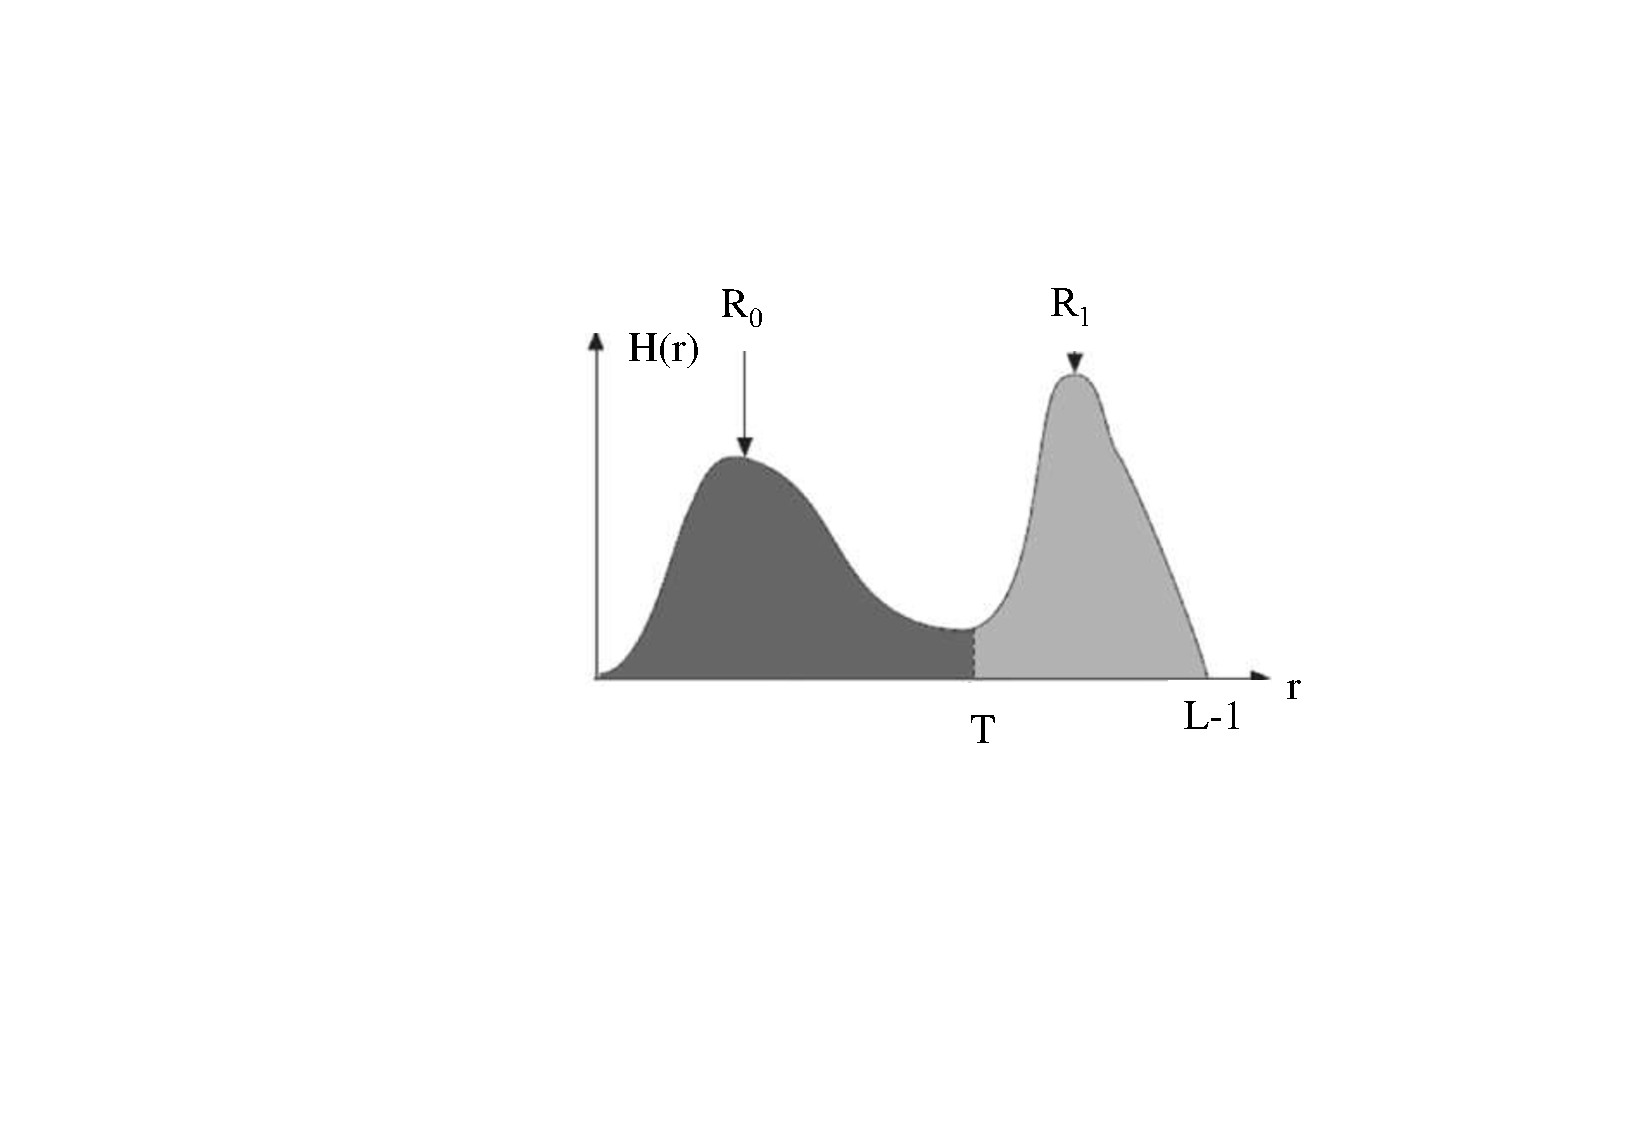
\includegraphics[width=0.5\textwidth]{img/binarizzazione_otsu.pdf}
	\end{figure}

	\noindent
	Se l'immagine ha un \textbf{istogramma bimodale la binarizzazione è efficace}, altrimenti no. Le due regioni sono definite come:
	
	\begin{equation*}
		\begin{array}{lll}
			p_{0 \rightarrow T}\left(r\right) & = & \dfrac{H\left(r\right)}{\displaystyle\sum_{r = 0}^{T} H\left(r\right)} \\
			&& \\
			\sigma_{0 \rightarrow T}^{2} & = & \displaystyle\sum_{r = 0}^{T} p_{0 \rightarrow T}\left(r\right)\left(r - \mu_{0 \rightarrow T}\right)^{2} \\
			&& \\
			\mu_{0 \rightarrow T} & = & \displaystyle\sum_{r = 0}^{T}r \cdot p_{0 \rightarrow T}\left(r\right)
		\end{array}
	\end{equation*}

	\noindent
	La formula \textbf{da minimizzare su $T$} è la seguente:
	
	\begin{equation*}
		\sigma_{w}^{2}\left(T\right) = W_{0}\left(T\right) \sigma_{0}^{2}\left(T\right) + W_{1}\left(T\right) \sigma_{1}^{2}\left(T\right)
	\end{equation*}

	\noindent
	Dove si considera la versione probabilistica dell'istogramma, ovvero la sua versione normalizzata, e si ha:
	
	\begin{equation*}
		\begin{array}{lll}
			W_{0}\left(T\right) & = & \displaystyle\sum_{r=0}^{T-1} p\left(r\right) \\
			&& \\
			W_{1}\left(T\right) & = & \displaystyle\sum_{r=T}^{L-1} p\left(r\right) \\
			&& \\
			p\left(r\right) & = & \dfrac{1}{M \cdot N} \displaystyle\sum_{r=0}^{L-1} H\left(r\right)
		\end{array}
	\end{equation*}

	\noindent
	Dove $W_{0}, W_{1}$ sono le probabilità che le due classi siano separate da $T$ e $\sigma_{0}^{2}$ e $\sigma_{1}^{2}$ sono le varianze sui valori di istogramma assunti dalle due classi. \textbf{L'approccio \dquotes{cicla} su tutti i possibili valori di $T$ e restituisce:}
	
	\begin{equation*}
		T_{best} = \arg_{T} \min \left(\sigma_{w}^{2}\left(T\right)\right)
	\end{equation*}

	\subsubsection{Equalizzazione}
	
	Un'immagine si dice \textbf{equalizzata} quando il contributo di ogni differente tonalità di grigio è simile. L'istogramma tende ad essere uniforme o appiattito.\newline
	
	\noindent
	L'\textbf{obbiettivo} è vedere l'istogramma come una distribuzione e di renderla il più simile a quella uniforme. Una \textbf{distribuzione uniforme} ha un'\textbf{entropia massima}\footnote{Secondo l'entropia, un sistema isolato si trasforma ed evolve nel tempo fino a raggiungere uno stato di equilibrio finale macroscopico in cui le differenze locali sono minime.}. Nelle immagini, ogni valore della distribuzione è un valore di grigio, per cui ogni valore di grigio appartiene all'entropia massima.\newline
	
	\noindent
	Si \textbf{utilizza} questo operatore poiché un istogramma piatto assicura a livello percettivo una risposta del cervello migliore (in termini di numero di dettagli che si riesce a riconoscere), per cui l'immagine diventa più \dquotes{informativa} da osservare.\newline
	
	\noindent
	Se $r_{k}$ è il $k$-esimo livello di grigio $k = 0, ..., L - 1$ e $H\left(r_{k}\right)$ è il conteggio dato dall'istogramma dell'immagine di dimensione $M \times N$, allora si può definire:
	
	\begin{equation*}
		p_{r}\left(r_{k}\right) = \dfrac{H\left(r_{k}\right)}{M \cdot N}
	\end{equation*}

	\noindent
	L'\textcolor{Red3}{\textbf{\underline{equalizzazione dell'istogramma}}} si basa sulla seguente funzione $T$, con $s_{k}$ che rappresenta il $k$-esimo valore di grigio in cui viene \dquotes{mappato} $r_{k}$:
	
	\begin{equation*}
		s_{k} = T\left(r_{k}\right) = \left(L-1\right) \displaystyle\sum_{j=0}^{k} p_{r}\left(r_{k}\right) = \dfrac{\displaystyle\sum_{j=0}^{k} H\left(r_{j}\right)}{\dfrac{M \cdot N}{\left(L-1\right)}}
	\end{equation*}

	\noindent
	\textcolor{Red3}{\textbf{\emph{\underline{Algoritmo}}}}
	
	\begin{enumerate}[label=\Roman*.]
		\item Calcolare le $L$ somme cumulative $\displaystyle\sum_{j=0}^{k} p_{r}\left(r_{j}\right)$ dei valori dell'istogramma visto come distribuzione con $k = 0, ..., L-1$;
		
		\item Moltiplicare i valori del passo precedente per il massimo di livelli di grigio $L - 1$;
		
		\item Normalizzazione dei valori calcolati al primo passo, dividendo per il numero totale di pixel $M \cdot N$ e arrotondamento;
		
		\item Applicare il mapping $T$ ottenuto.
	\end{enumerate}

	\newpage
	
	\noindent
	\textcolor{Green4}{\textbf{\underline{\emph{Esempio}}}}\newline
	
	\noindent
	Sia data un'immagine con $L = 8, 64\times64$ pixel $\left(M \cdot N = 4096\right)$, con la seguente distribuzione d'intensità:
	
	\begin{table}[!htbp]
		\centering
		\begin{tabular}{@{} l c c @{}}
			\toprule
			$r_{k}$ & $H\left(r_{k}\right)$ & $p_{r}\left(r_{k}\right) = \dfrac{H\left(r_{k}\right)}{M \cdot N}$ \\
			\midrule
			$r_{0} = 0$	& $790$	& $0.19$ \\
			&& \\
			$r_{1} = 1$	& $1023$& $0.25$ \\
			&& \\
			$r_{2} = 2$	& $850$	& $0.21$ \\
			&& \\
			$r_{3} = 3$	& $656$	& $0.16$ \\
			&& \\
			$r_{4} = 4$	& $329$	& $0.08$ \\
			&& \\
			$r_{5} = 5$	& $245$	& $0.06$ \\
			&& \\
			$r_{6} = 6$	& $122$	& $0.03$ \\
			&& \\
			$r_{7} = 7$	& $81$	& $0.02$ \\
			\bottomrule
		\end{tabular}
	\end{table}

	\begin{figure}[!htp]
		\centering
		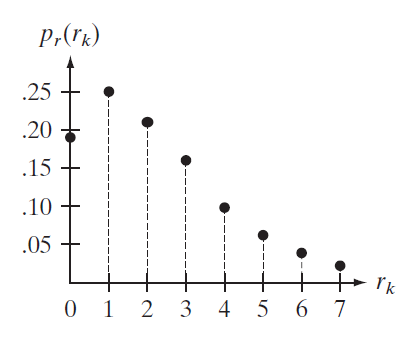
\includegraphics[width=0.5\textwidth]{img/eg_equalizzazione.png}
		\caption{Rappresentazione della distribuzione di intensità.}
	\end{figure}
	
	\noindent
	Si applica la formula di equalizzazione:
	
	\begin{equation*}
		\begin{array}{lllllllll}
			s_{0} & = & T\left(r_{0}\right) & = & 7\displaystyle\sum_{j=0}^{0} p_{r}\left(r_{j}\right) & = & 7p_{r}\left(r_{0}\right) & = & 1.33 \\
			&&&&&&&&\\
			s_{1} & = & T\left(r_{1}\right) & = & 7\displaystyle\sum_{j=0}^{1} p_{r}\left(r_{j}\right) & = & 7p_{r}\left(r_{0}\right) + 7p_{r}\left(r_{1}\right) & = & 3.08
		\end{array}
	\end{equation*}
	
	\noindent
	Analogamente anche per gli altri valori si applica la formula e si trovano i seguenti valori:
	
	\begin{equation*}
		\begin{array}{lll}
			s_{2} & = & 4.55 \\
			s_{3} & = & 5.67 \\
			s_{4} & = & 6.23 \\
			s_{5} & = & 6.65 \\
			s_{6} & = & 6.86 \\
			s_{7} & = & 7.00 \\
		\end{array}
	\end{equation*}

	\begin{figure}[!htp]
		\centering
		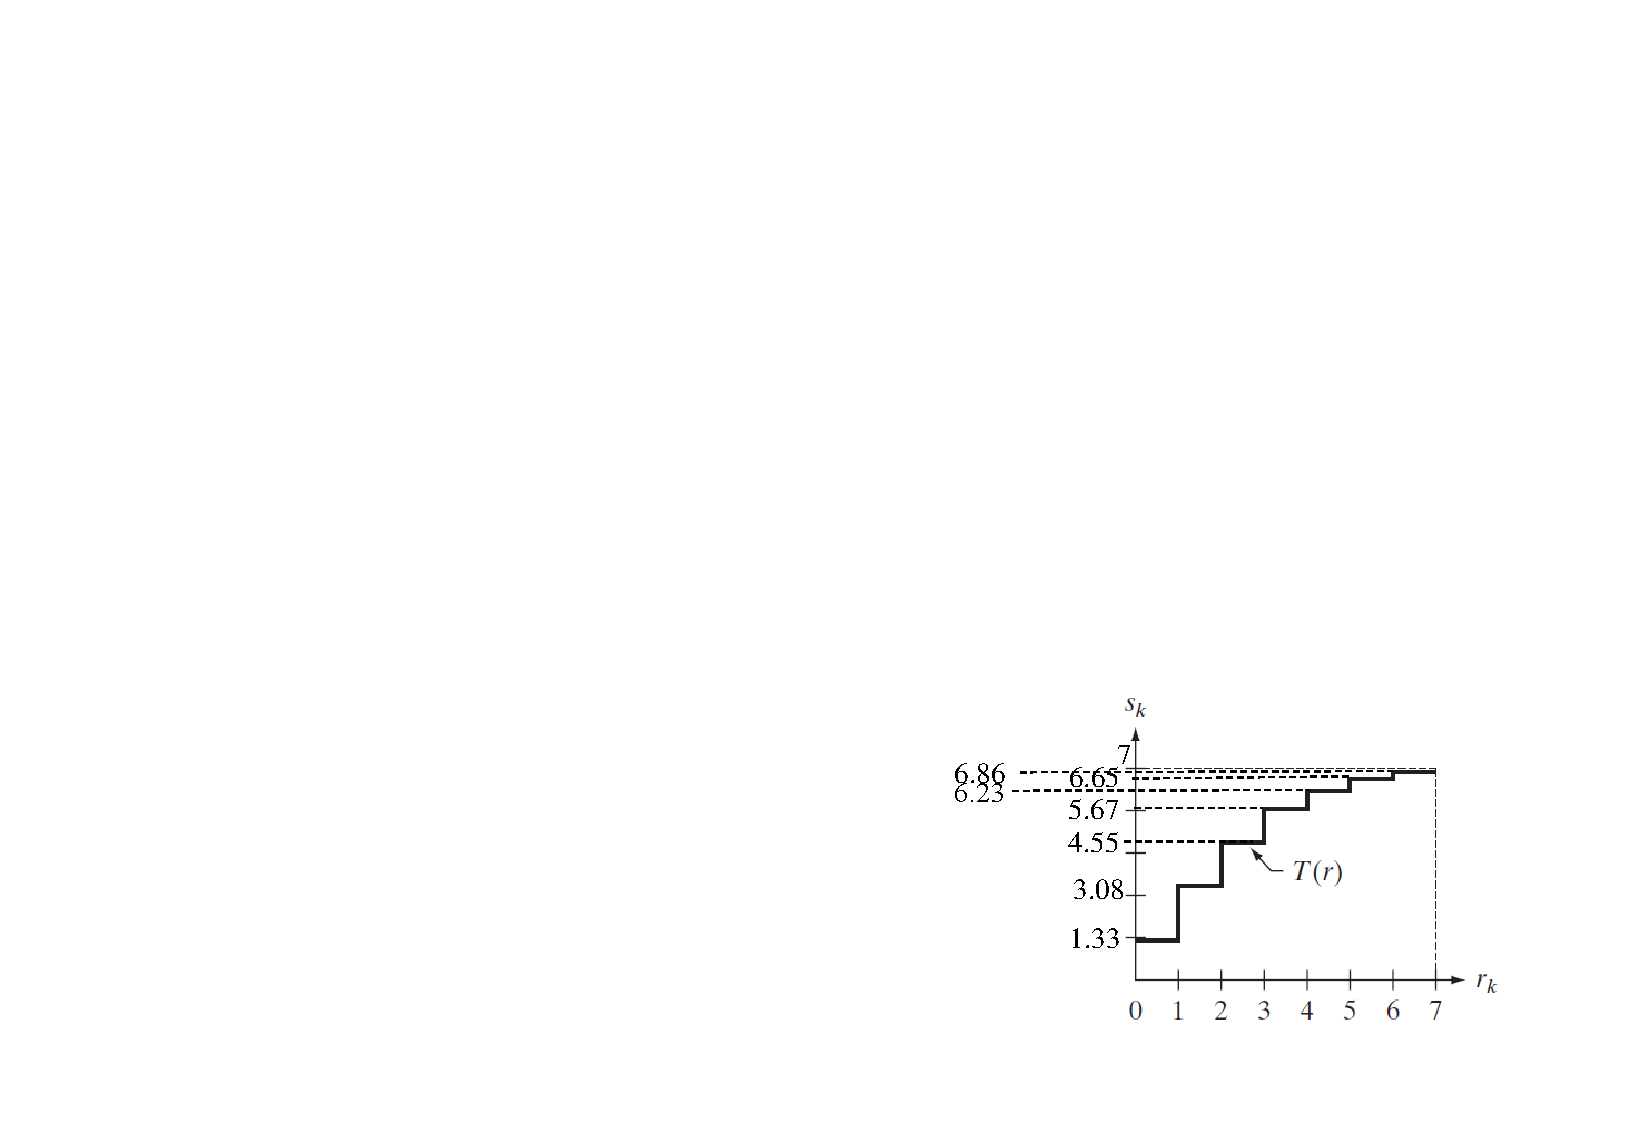
\includegraphics[width=0.7\textwidth]{img/eg_equalizzazione.pdf}
		\caption{LUT (\emph{Lookup Table})}
	\end{figure}

	\noindent
	\textbf{LUT} (\emph{Lookup Table}) è un termine utilizzato per descrivere una predeterminata lista di numeri che offre una \dquotes{scorciatoia} per una specifica computazione. Nel contesto dei colori, una LUT trasforma i colori, ricevuti come input (camera), in un output desiderato (final footage).\newline
	
	\noindent
	L'immagine è quantizzata, quindi si effettua l'arrotondamento dei valori ottenendo l'intero più vicino:
	
	\begin{equation*}
		\begin{array}{lllll}
			s_{0} & = & 1.33 & \longrightarrow & 1 \\
			s_{1} & = & 3.08 & \longrightarrow & 3 \\
			s_{2} & = & 4.55 & \longrightarrow & 5 \\
			s_{3} & = & 5.67 & \longrightarrow & 6 \\
			s_{4} & = & 6.23 & \longrightarrow & 6 \\
			s_{5} & = & 6.65 & \longrightarrow & 7 \\
			s_{6} & = & 6.86 & \longrightarrow & 7 \\
			s_{7} & = & 7.00 & \longrightarrow & 7 \\
		\end{array}
	\end{equation*}

	\newpage

	\noindent
	Dopo l'arrotondamento, si ottiene una nuova immagine e il suo relativo istogramma.
	
	\begin{figure}[!htp]
		\centering
		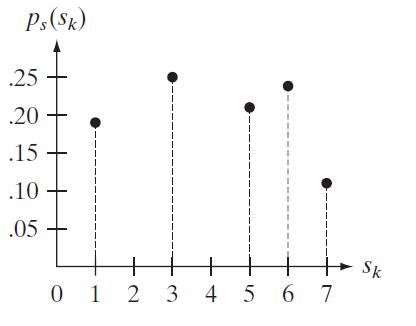
\includegraphics[width=0.5\textwidth]{img/eg_equalizzazione2.png}
	\end{figure}

	\newpage
	
	\subsection{Operazioni locali}
	
	Un'\textcolor{Red3}{\textbf{\underline{operazione locale}}} restituisce un pixel che dipende da un limitato intorno del corrispondente punto in input. Tali operazioni vengono \textbf{utilizzati} per migliorare la qualità delle immagini o per estrarre delle informazioni dall'immagine.\newline
	
	\noindent
	Le operazioni locali sono come dei filtraggi spaziali dell'immagine. Il \textbf{\underline{filtraggio spaziale}} è un'elaborazione $T$ dell'immagine $f$ dove un pixel di locazione $\left(n,m\right)$, di intensità $f\left(n,m\right)$, viene cambiato in $g\left(n,m\right)$ da una funzione dei pixel in un intorno di $\left(n,m\right)$, ossia:
	
	\begin{equation*}
		g\left(n,m\right) = T\left(\left[f\left(n,m\right)\right]\right)
	\end{equation*}

	\noindent
	Dove le parentesi quadrate indicano che viene preso in considerazione un intorno di $n,m$. Ovviamente, il risultato dell'operazione, se applicato a tutti i pixel dell'immagine $f$, è una nuova immagine $g$.\newline
	
	\noindent
	Gli intorni presi maggiormente in considerazione sono di grandezza $K \times K$, con $K$ dispari (per fare in modo di considerare uniformemente i pixel attorno al punto $\left(n,m\right)$ di applicazione), di solito $3 \times 3, 5 \times 5, 7 \times 7$. I pixel al di fuori dell'intorno non prendono parte alla funzione.\newline
	
	\noindent
	\textcolor{Red3}{\textbf{\underline{\emph{Pseudocodice}}}}\newline
	
	\begin{itemize}
		\item \textbf{Input:}
		\begin{itemize}
			\item Immagine $f$ definita con un suo valore di pixel generico $f\left(n,m\right) \in \left[0 ... L - 1\right] \subset \mathbb{N}$ con $\left(n,m\right) \in \left[1 ... \mathbb{N}\right] \times \left[1 ... M\right] \subset \mathbb{N} \times \mathbb{N}$;
			
			\item Intorno di valori di pixel $\left[f\left(n,m\right)\right]$ ossia $f\left(n-u, m-v\right)$ definita come:
			\begin{equation*}
				\left(u,v\right) \in \left[-\dfrac{K-1}{2} \cdots \dfrac{K-1}{2}\right] \times \left[-\dfrac{K-1}{2} \cdots \dfrac{K-1}{2}\right] \subset \mathbb{N} \times \mathbb{N} \hspace{2em} K \in \left\{3,5,7,...\right\}
			\end{equation*}
		\end{itemize}
		
		\item \textbf{Output:}
		\begin{itemize}
			\item Nuova immagine $g\left(n,m\right) \in \mathbb{R}$ che attraverso operazioni puntuali può essere riportata in $g\left(n,m\right) \in \left[0 ... L-1\right] \subset \mathbb{N}$
		\end{itemize}
	
		\item \textbf{Procedimento:}
		\begin{equation*}
			\begin{array}{l}
				\mathrm{for} \: n = 1 ... N \\
				\hspace{2em} \mathrm{for} \: m = 1 ... M \\
				\hspace{4em} g\left(n,m\right) = T\left(\left[f\left(n,m\right)\right]\right)
			\end{array}
		\end{equation*}
	\end{itemize}

	\newpage
	
	\subsubsection{Filtraggi spaziali: lineari e non lineari}
	
	Le due principali categorie di operazioni locali sono lineari e non lineari:
	
	\begin{itemize}
		\item \textcolor{Red3}{\textbf{\underline{Filtraggio lineare}}} se $T$ è una combinazione lineare dei valori di pixel nel vicinato. Quindi, la convoluzione di un'immagine con un kernel è una somma di fattori ognuno dei quali è una moltiplicazione di un valore dell'immagine per un coefficiente del filtro:
		\begin{equation*}
			g\left(n,m\right) = T\left(\left[f\left(n,m\right)\right]\right) = h * f\left(n,m\right) = \sum_{u=-k}^{+k} \sum_{v=-k}^{+k} h\left(u,v\right) f\left(n-u, m-v\right)
		\end{equation*}
		\begin{equation*}
			k = \dfrac{K-1}{2}
		\end{equation*}
		Un esempio di operazione lineare è la convoluzione;
		
		\item \textcolor{Red3}{\textbf{\underline{Filtraggio non lineare}}} se $T$ contiene operazioni non lineari sulle variabili indipendenti. Un esempio di operazioni non lineari sono la mediana dei pixel nell'intorno e il valore massimo dei pixel nel vicinato.
	\end{itemize}

	\noindent
	I filtraggi lineari \textbf{\underline{non}} presentano un \textbf{\underline{problema ai bordi}} nel momento in cui l'intorno è definito all'interno dell'immagine (cioè non cade fuori dall'immagine). Alcuni filtri lineari:
	
	\begin{itemize}[label=-]
		\item \textbf{Cropping} è un filtro dove solo l'intorno cade all'interno dell'immagine, quindi il filtro viene applicato ad un'area ristretta e non a tutta l'immagine. Un esempio:
		\begin{equation*}
			\text{Input } = 
			\begin{bmatrix}
				1 & 2 & 2 & 3 & 1 \\
				3 & 2 & 2 & 1 & 4 \\
				2 & 5 & 2 & 7 & 1 \\
				9 & 0 & 1 & 1 & 2 \\
				3 & 1 & 2 & 4 & 1
			\end{bmatrix}
			\longrightarrow
			\text{ Output } = 
			\begin{bmatrix}
				* & * & * & * & * \\
				* & 30 & 45 & 30 & * \\
				* & 46 & 27 & 37 & * \\
				* & 34 & 41 & 28 & * \\
				* & * & * & * & *
			\end{bmatrix}
		\end{equation*}
		Le aree con un * non verranno calcolate;
		
		\item \textbf{Zero Padding} utilizzato per inserire degli zero che creano degli artefatti così da consentire il filtraggio. Un esempio:
		\begin{equation*}
			\text{Input } = 
			\begin{bmatrix}
				0 & 0 & 0 & 0 & 0 & 0 & 0 \\
				0 & 1 & 2 & 2 & 3 & 1 & 0 \\
				0 & 3 & 2 & 2 & 1 & 4 & 0 \\
				0 & 2 & 5 & 2 & 7 & 1 & 0 \\
				0 & 9 & 0 & 1 & 1 & 2 & 0 \\
				0 & 3 & 1 & 2 & 4 & 1 & 0 \\
				0 & 0 & 0 & 0 & 0 & 0 & 0
			\end{bmatrix}
			\longrightarrow
			\text{ Output } = 
			\begin{bmatrix}
				\colorbox{gray}{11} & \colorbox{gray}{19} & \colorbox{gray}{17} & \colorbox{gray}{22} & \colorbox{gray}{11} \\
				\colorbox{gray}{25} & 30 & 45 & 30 & \colorbox{gray}{31} \\
				\colorbox{gray}{25} & 46 & 27 & 37 & \colorbox{gray}{19} \\
				\colorbox{gray}{35} & 34 & 41 & 28 & \colorbox{gray}{29} \\
				\colorbox{gray}{16} & \colorbox{gray}{27} & \colorbox{gray}{12} & \colorbox{gray}{18} & \colorbox{gray}{10}
			\end{bmatrix}
		\end{equation*}
		Le aree in grigio non vengono calcolate.
		
		\newpage
		
		\item \textbf{Replicazione} utilizzata per creare artefatti, infatti l'immagine risultante non è realistica. Un esempio:
		\begin{equation*}
			\text{Input } = 
			\begin{bmatrix}
				1 & 1 & 2 & 2 & 3 & 1 & 1 \\
				1 & 1 & 2 & 2 & 3 & 1 & 1 \\
				3 & 3 & 2 & 2 & 1 & 4 & 4 \\
				2 & 2 & 5 & 2 & 7 & 1 & 1 \\
				9 & 9 & 0 & 1 & 1 & 2 & 2 \\
				3 & 3 & 1 & 2 & 4 & 1 & 1 \\
				3 & 3 & 1 & 2 & 4 & 1 & 1
			\end{bmatrix}
			\longrightarrow
			\text{ Output } = 
			\begin{bmatrix}
				\colorbox{gray}{25} & \colorbox{gray}{27} & \colorbox{gray}{29} & \colorbox{gray}{31} & \colorbox{gray}{33} \\
				\colorbox{gray}{34} & 30 & 45 & 30 & \colorbox{gray}{39} \\
				\colorbox{gray}{51} & 46 & 27 & 37 & \colorbox{gray}{32} \\
				\colorbox{gray}{54} & 34 & 41 & 28 & \colorbox{gray}{35} \\
				\colorbox{gray}{48} & \colorbox{gray}{32} & \colorbox{gray}{24} & \colorbox{gray}{34} & \colorbox{gray}{26}
			\end{bmatrix}
		\end{equation*}
		Le aree in grigio non vengono calcolate.
	\end{itemize}

	\newpage
	
	\subsection{Rumore nelle immagini}
	
	Il \textcolor{Red3}{\textbf{\underline{rumore nelle immagini}}} è un disturbo dell'immagine introdotto dal sistema di acquisizione (e.g. fotocamera) o dal mezzo di propagazione che ne degrada la qualità (e.g. Whatsapp). Il rumore è tipicamente \emph{modellato} come \textbf{additivo} e \textbf{casuale}:
	
	\begin{equation*}
		\tilde{f}\left(n,m\right) = f\left(n,m\right) + \varepsilon\left(n,m\right)
	\end{equation*}

	\noindent
	Dove $f$ è l'\textbf{immagine} priva di rumore e $\varepsilon$ è un processo aleatorio che genera delle quantità che seguono una distribuzione particolare, indipendentemente da dove il processo è collocato nell'immagine, ovvero indipendentemente da $n,m$.\newline
	
	\noindent
	Esistono due \textbf{tipi di rumore}: gaussiano additivo bianco (rumore generato da una distribuzione gaussiana) e impulsivo (rumore generato da una distribuzione bernoulliana).\newline
	
	\noindent
	La \textbf{quantità di rumore} può essere stimata attraverso la misura di $SNR$\label{SNR} (\emph{signal to noise ratio}), di cui esistono varie versioni. La più utilizzata è la \emph{\textbf{mean square, $SNR_{ms}$}}:
	
	\begin{equation*}
		SNR_{ms} = \dfrac{
		\displaystyle\sum_{n=1}^{N}\sum_{m=1}^{M} \tilde{f}\left(n,m\right)^{2}
		}{
		\displaystyle\sum_{n=1}^{N}\sum_{m=1}^{M} \left[\tilde{f}\left(n,m\right) - f\left(n,m\right)\right]^{2}
		}
	\end{equation*}

	\noindent
	Una forma alternativa della $SNR$ può essere stimata grazie alla varianza $\sigma_{n}^{2}$, o alla deviazione standard $\sigma_{n}$:
	
	\begin{equation*}
		SNR = \dfrac{\sigma_{s}}{\sigma_{n}}
	\end{equation*}

	\noindent
	Dove $\sigma_{s}$ è la deviazione standard del segnale e $\sigma_{n}$ è la deviazione standard dell'immagine affetta da rumore. Per questo motivo si utilizzano immagini ad alto contrasto, poiché $\sigma_{s}$ risulta maggiore!
	
	\newpage
	
	\subsubsection{Rumore gaussiano additivo bianco}
	
	Il \textcolor{Red3}{\textbf{\underline{rumore gaussiano additivo bianco}}} è un processo stocastico, ovvero una variabile aleatoria che emette valori casuali nel tempo $\varepsilon\left(t\right)$ o nello spazio $\varepsilon\left(n,m\right)$ con le seguenti caratteristiche:
	
	\begin{itemize}
		\item Si somma al segnale pulito;
		
		\item Non è periodico nel tempo o nello spazio;
		
		\item I valori vengono prodotti con la seguente probabilità:
		\begin{equation*}
			P\left(\varepsilon\left(n,m\right) = l\right) = \dfrac{1}{\sqrt{2\pi\sigma^{2}}} \cdot \exp\left(-\dfrac{\left(l - 0\right)^{2}}{2\sigma^{2}}\right)
		\end{equation*}
		In cui $0$ è uguale a $\mu$, ovvero indica la media del rumore. Inoltre, data una distribuzione gaussiana $\mu$, $\sigma^{2}$ il $98\%$ di valori $l \in \left[\mu - 2.5\sigma, \mu + 2.5\sigma\right]$.
		
		\item I valori seguono una distribuzione gaussiana di media pari a zero, ed una particolare varianza $\sigma^{2}$ (o deviazione standard $\sigma$) dove più è alta la varianza, più distanti da zero saranno i numeri prodotti e sommati all'immagine pulita, più rumorosa l'immagine finale.
	\end{itemize}

	\begin{figure}[!htp]
		\centering
		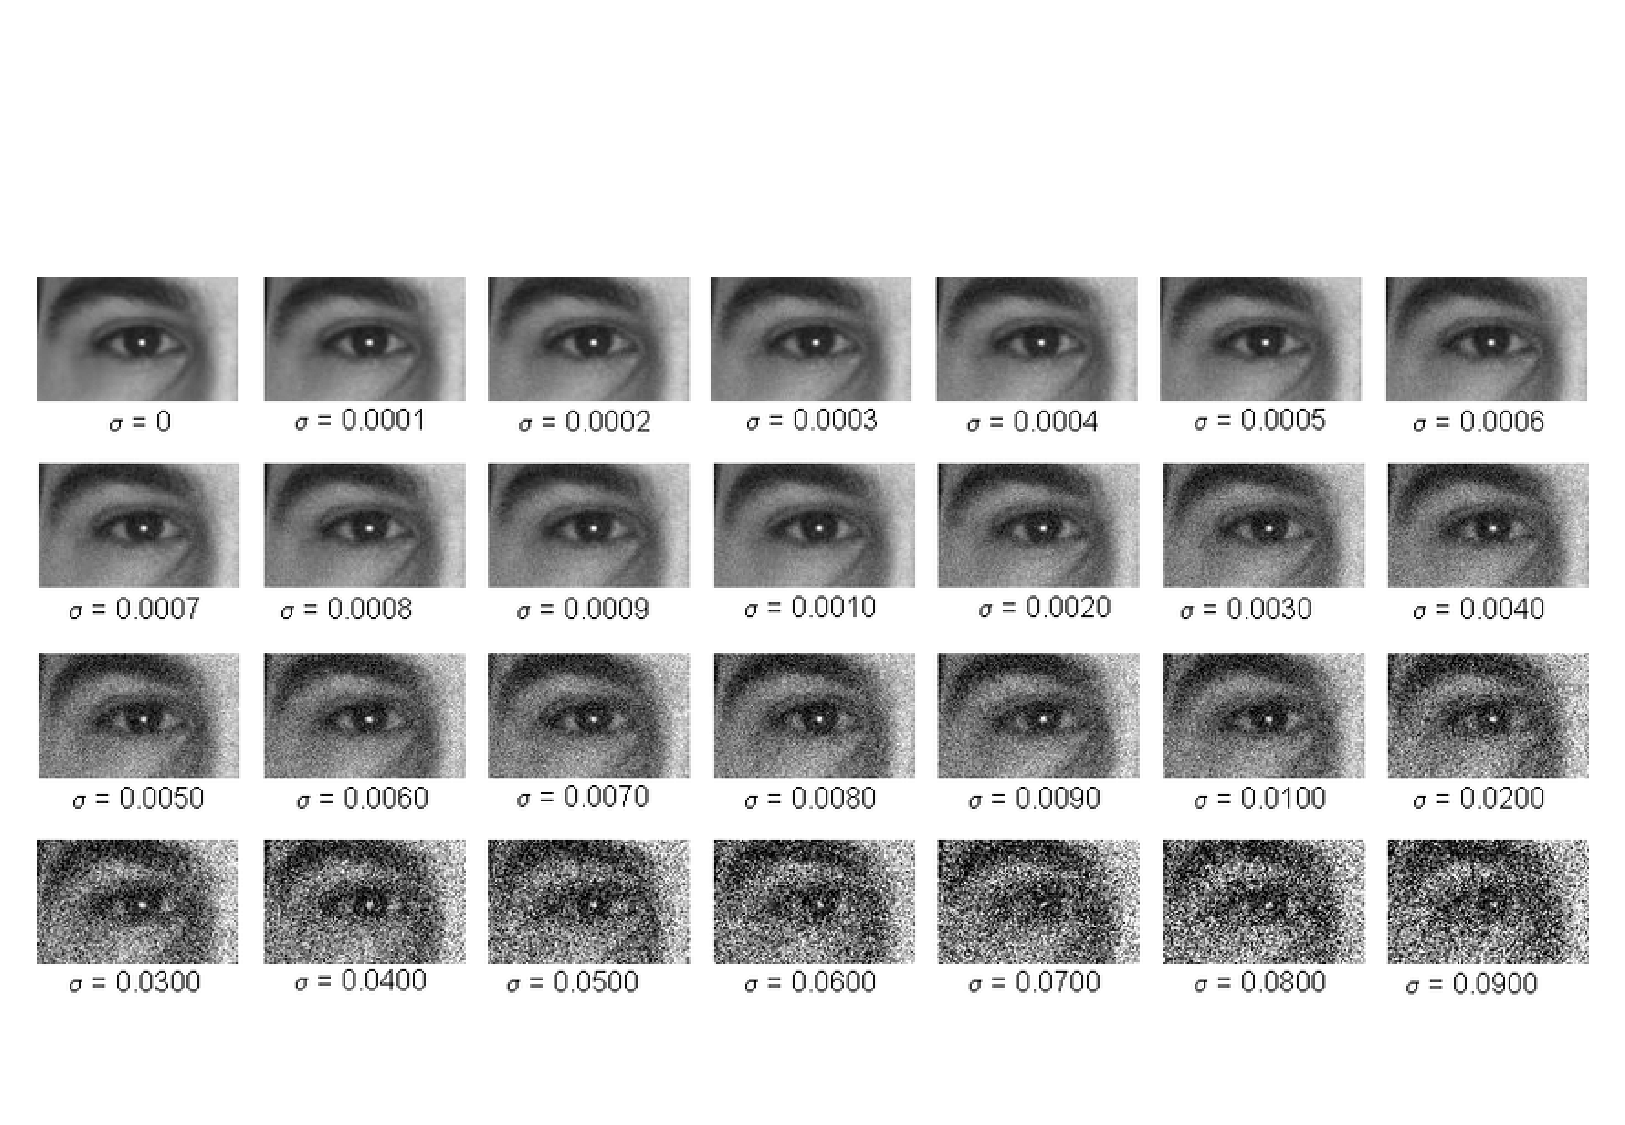
\includegraphics[width=\textwidth]{img/rumore_gaussiano_additivo_bianco.pdf}
		\caption{Esempio di rumore gaussiano a diversi valori di $\sigma$.}
	\end{figure}

	\newpage
	
	\subsubsection{Rumore impulsivo}
	
	Il \textcolor{Red3}{\textbf{\underline{rumore impulsivo}}} è causato da alterazione brusche nel segnale, viene parametrizzato da un fattore $D$ (una percentuale) che è la densità con cui esso si localizza su pixel dell'immagine: maggiore il valore di intensità $D$, maggiore sarà il numero di pixel affetti.\newline
	
	\noindent
	Per esempio, il disturbo sale e pepe (\href{https://it.wikipedia.org/wiki/Rumore_sale_e_pepe}{\emph{salt-and-pepper noise}}) può essere utilizzato selezionando una percentuale $D$ di pixel, ovvero $D\%$, in maniera uniforme nell'immagine e per ogni pixel si assegna un valore minimo o massimo con probabilità uniforme pari a $p = 0.5$.
	
	\begin{figure}[!htp]
		\centering
		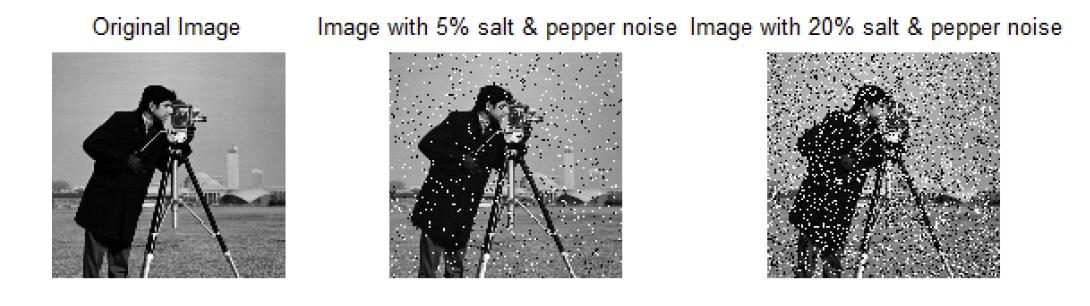
\includegraphics[width=\textwidth]{img/rumore_impulsivo.png}
		\caption{Esempio di applicazione dell'effetto \emph{salt-and-pepper noise}.}
	\end{figure}

	\newpage
	
	\subsection{Altre operazioni locali: tipologie di filtraggio}
	
	Esistono altre $3$ tipologie principali di filtraggio:
	
	\begin{itemize}
		\item \textcolor{Red3}{\textbf{\emph{Smoothing}}}, utilizzato per aumentare il $SNR$ (pagina~\pageref{SNR}), ovvero per rimuovere il rumore.\newline
		Per esempio, il filtro di media, mediano, gaussiano;

		\item \textcolor{Red3}{\textbf{\emph{Sharpening}}}, utilizzato per aumentare il grado di dettaglio delle immagini.\newline
		Per esempio, il filtro laplaciano;

		\item \textcolor{Red3}{\textbf{\emph{Estrazione di caratteristiche}}}, utilizzato per estrarre rappresentazioni alternative alle immagini di partenza, che ne evidenzino aspetti particolari (edge, microstrutture, oggetti).\newline
		Per esempio, il filtro prewitt, sobel, cenny.
	\end{itemize}

	\newpage

	\subsubsection{Smoothing - Filtro media}
	
	Il \textcolor{Red3}{\textbf{\underline{filtro media}}} è utilizzato per \textbf{rimuovere il rumore gaussiano}. È un filtraggio $T$ lineare, si attua attraverso la convoluzione dell'immagine con la maschera media la quale ha le seguenti caratteristiche:
	
	\begin{itemize}[label=-]
		\item Dimensioni $K \times K$ con $K$ dispari;
		\item I suoi coefficienti sono tutti uguali e pari a $\dfrac{1}{K^{2}}$;
		\item Il suo funzionamento è il seguente: dato un intorno di applicazione $\left[\left(n,m\right)\right]$, esso calcola la media dei valori vii compresi $\left[\tilde{f}\left(n,m\right)\right]$, e la sostituisce al posto del valore $\tilde{f}\left(n,m\right)$:
		\begin{equation*}
			g\left(n,m\right) = T\left(\left[\tilde{f}\left(n,m\right)\right]\right) = E\left(\left[f\left(n,m\right)\right]\right)
		\end{equation*}
		Dove $E$ è l'operatore di media, perché $T$ essenzialmente è l'operatore di media
	\end{itemize}

	\noindent
	Si \textbf{osservi} che la somma dei valori del kernel è $1$:
	
	\begin{equation*}
		\begin{bmatrix}
			\frac{1}{9} & \frac{1}{9} & \frac{1}{9} \\
			&& \\
			\frac{1}{9} & \frac{1}{9} & \frac{1}{9} \\
			&& \\
			\frac{1}{9} & \frac{1}{9} & \frac{1}{9}
		\end{bmatrix}
	\end{equation*}

	\noindent
	Questo significa che il filtraggio in una locazione $\left(x,y\right)$ è una \textbf{combinazione lineare convessa}. In altre parole, la somma dei livelli di grigio dell'immagine originale $f$ e di quella processata $g$ sono uguali (a meno di padding!).\newline
	\textbf{Maggiore è l'ampiezza} $K$ della maschera, \textbf{più severo è l'effetto della media} sulla struttura dell'immagine.
	
	\begin{figure}[!htp]
		\centering
		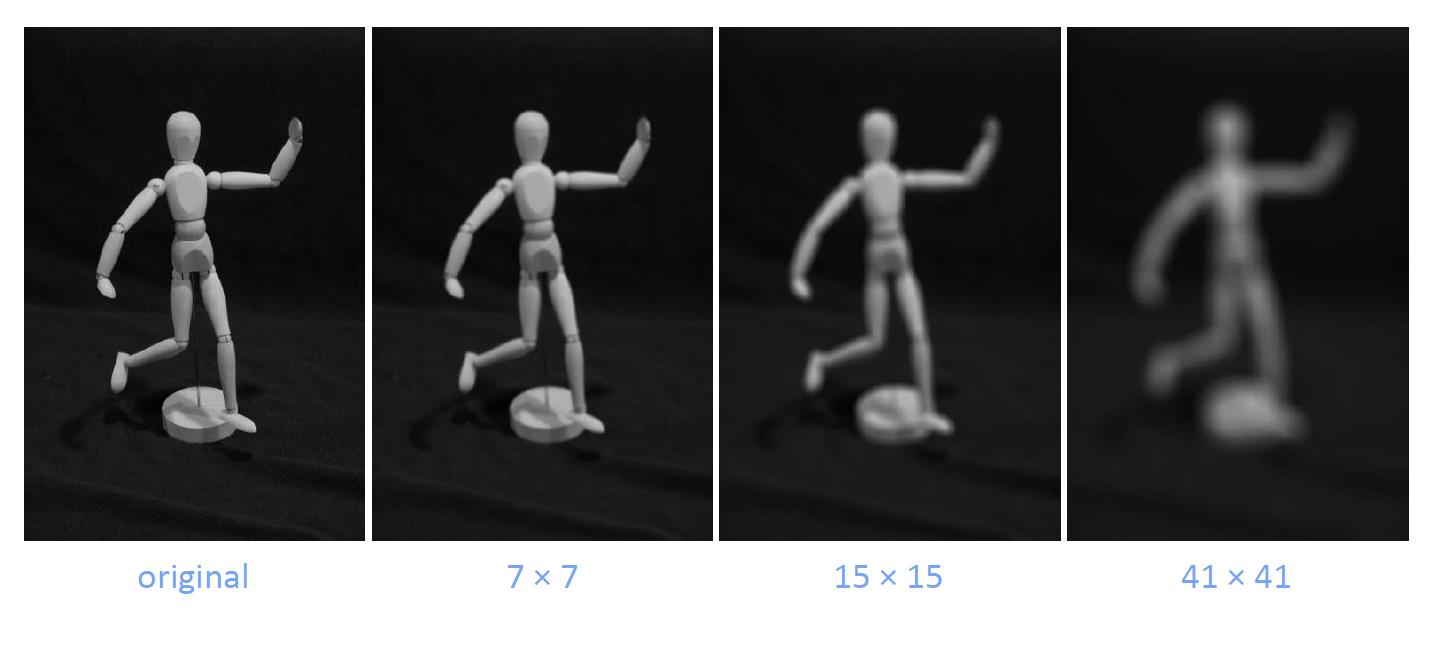
\includegraphics[width=\textwidth]{img/filtro_media.png}
		\caption{Esempio di filtro media all'aumentare di $K$, ovvero della grandezza.}
	\end{figure}

	\subsubsection{Smoothing - Filtro mediano}
	
	Il \textcolor{Red3}{\textbf{\underline{filtro mediano}}} è utilizzato per \textbf{rimuovere il rumore impulsivo}. È un filtraggio $T$ non lineare, che si realizza attraverso un algoritmo. Data la matrice dell'immagine:
	
	\begin{equation*}
		\begin{bmatrix}
			240 & 245 & 0   \\
			247 & 0   & 244 \\
			251 & 246 & 250
		\end{bmatrix}
	\end{equation*}

	\begin{enumerate}
		\item Si calcola la media di tutti i valori della matrice:
		\begin{equation*}
			\dfrac{240+245+0+247+0+244+251+246+250}{9} \approx 191
		\end{equation*}
	
		\item Si inseriscono in un vettore riga i valori in ordine crescente:
		\begin{equation*}
			\begin{bmatrix}
				0 & 0 & 240 & 244 & 245 & 246 & 247 & 250 & 251
			\end{bmatrix}
		\end{equation*}
	
		\item Si calcola la mediana del vettore:
		\begin{equation*}
			9 \div 2 = 4.5 \longrightarrow \begin{bmatrix}
				0 & 0 & 240 & 244 & \underline{245} & 246 & 247 & 250 & 251
			\end{bmatrix}
		\end{equation*}
	\end{enumerate}

	\begin{figure}[!htp]
		\centering
		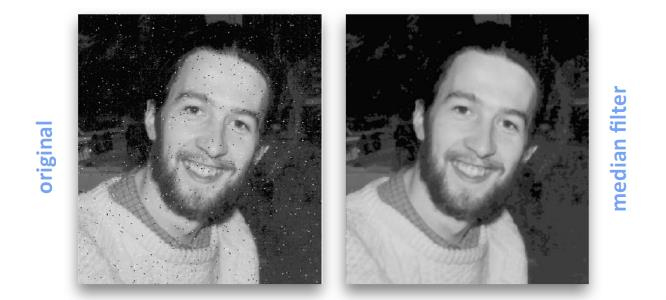
\includegraphics[width=\textwidth]{img/filtro_mediano.png}
		\caption{Esempio di applicazione di filtro mediano.}
	\end{figure}

	\newpage
	
	\subsubsection{Smoothing - Filtro gaussiano}
	
	Il \textcolor{Red3}{\textbf{\underline{filtro gaussiano}}} è quello di rendere più \dquotes{lisica (\emph{smooth})} l'immagine, in modo simile al filtraggio di media, e come parametro l'operatore prende il valore $\sigma$ che rappresenta la \textbf{forza} (maggiore è il valore, più è forte lo \emph{smoothing}). La \textbf{differenza} sostanziale tra il filtraggio di media e il filtraggio gaussiano è che quest'ultimo è una media pesata, dove i pesi più vicini al centro della maschera hanno valori più alti. Così facendo si ha:
	
	\begin{itemize}
		\item \textcolor{Green4}{\textbf{\emph{Vantaggio}}}
		\begin{itemize}
			\item Il filtraggio gaussiano effettua uno \emph{smoothing} più lieve, \textbf{preservando i contorni meglio} di quanto faccia il filtraggio media. Quindi, la struttura viene preservata meglio.
		\end{itemize}
		
		\item \textcolor{Red3}{\textbf{\emph{Svantaggio}}}
		\begin{itemize}
			\item Il rumore viene rimosso in maniera inferiore e questo provoca l'\textbf{impossibilità di applicare la formula di annullamento del rumore} visto per il filtro media.
		\end{itemize}
	\end{itemize}

	\noindent
	Questo filtro può essere \textbf{implementato in maniera efficiente} in quanto la maschera è separabile, ovvero è possibile eseguirlo facendo un filtraggio prima su tutte le $N$ righe dell'immagine come se fossero funzioni $1D$, e poi su tutte le $M$ colonne:
	
	\begin{equation*}
		\begin{array}{lll}
			I_{G}\left(i,j\right) & = & \displaystyle\sum_{h = -\frac{m}{2}}^{\frac{m}{2}} \displaystyle\sum_{k = -\frac{m}{2}}^{\frac{m}{2}} G\left(h,k\right) I\left(i+h, j+k\right) \\
			&& \\
			& = & \displaystyle\sum_{h = -\frac{m}{2}}^{\frac{m}{2}} \displaystyle\sum_{k = -\frac{m}{2}}^{\frac{m}{2}} \exp\left(-\dfrac{h^{2} + k^{2}}{2\sigma^{2}}\right) I\left(i+h, j+k\right) \\
			&& \\
			& = & \displaystyle\sum_{h = -\frac{m}{2}}^{\frac{m}{2}} \exp\left(-\dfrac{h^{2}}{2\sigma^{2}}\right) \displaystyle\sum_{k = - \frac{m}{2}}^{\frac{m}{2}} \exp\left(-\dfrac{k^{2}}{2\sigma^{2}}\right) I\left(i+h, j+k\right)
		\end{array}
	\end{equation*}

	\noindent
	Dove le variabili $i,j,h,k,m$ sono indici per comprendere la \textbf{separabilità}. Quest'ultima consente di progettare manualmente un filtro gaussiano come segue nella prossima pagina.
	
	\newpage
	
	\noindent
	Si definiscono i parametri $\sigma$ e $W$. Quindi, si fissi $\sigma$ e si trovi la dimensione della maschera $W$ sapendo che $W$ deve essere tale da contenere un'elevata percentuale di probabilità (uguale all'area della densità gaussiana, come in figura). In particolare, la statistica dice che con $W = 5\sigma$ si copre il $98.75\%$ dell'area della densità gaussiana. In altre parole, se si vuole $\sigma = 1$ allora $W = 5 \cdot 1 = 5$; se si vuole $\sigma = 0.6$ allora $W = 5 \cdot 0.6 = 3$.
	
	\begin{figure}[!htp]
		\centering
		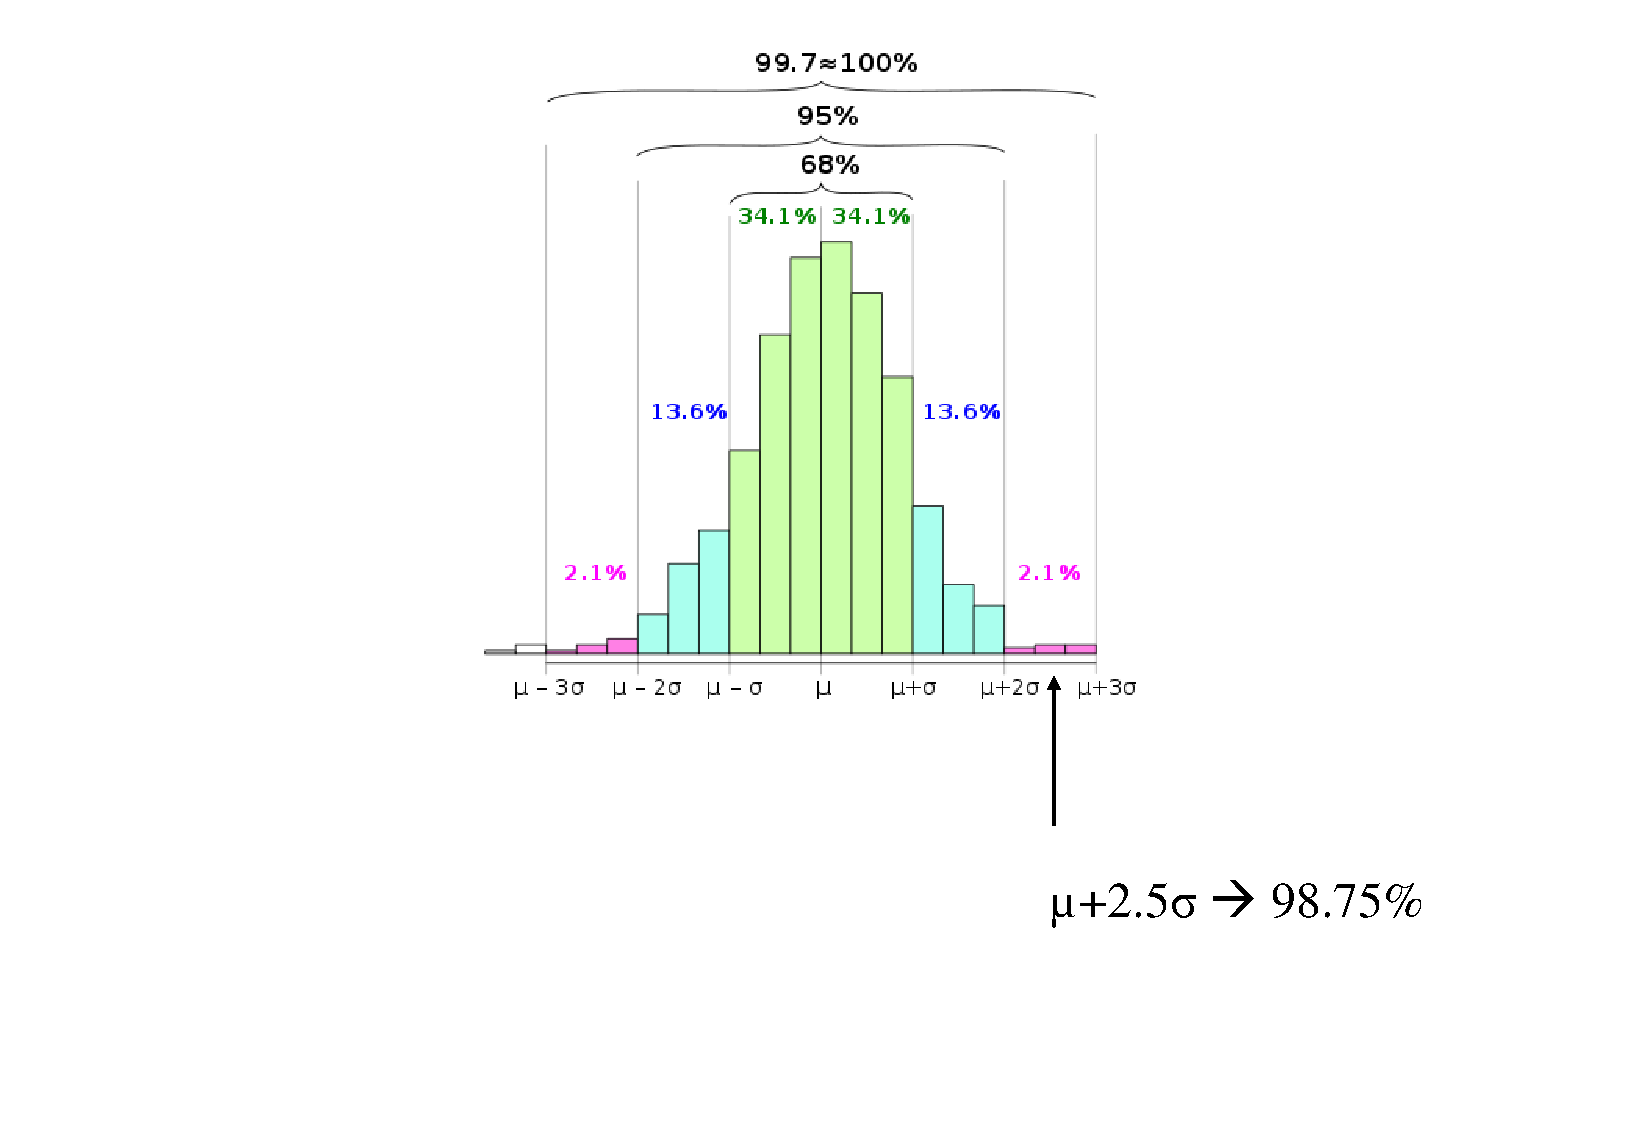
\includegraphics[width=\textwidth]{img/filtro_gaussiano.pdf}
	\end{figure}

	\subsubsection{Domanda da \textcolor{Red3}{esame}}
	
	\textcolor{Red3}{\textbf{\emph{Domanda}}}\newline
	
	\noindent
	Il livello di noise gaussiano presente in un'immagine, se esso noto (e.g. $\sigma_{1} = 0.01$) può guidare la scelta del parametro $\sigma_{2}$ della maschera di filtro gaussiano?\newline
	
	\noindent
	\textcolor{Green4}{\textbf{\emph{Risposta}}}\newline
	
	\noindent
	No, perché il rumore gaussiano lavora su tutti i valori di grigio, mentre il filtro gaussiano sulle coordinate e non c'è correlazione. Invece, il filtro media è quello ideale.
	
	\newpage
	
	\subsubsection{Filtraggi di sharpening}
	
	I \textcolor{Red3}{\textbf{\underline{filtraggi di sharpening}}} servono per evidenziare i dettagli o come post processing dopo filtraggi di \emph{smoothing} (questo perché i filtraggi di \emph{smoothing} eliminano i dettagli). Per lo stesso motivo, i filtraggi di sharpening possono incrementare il rumore (un'immagine di rumore è un'immagine ad alta frequenza). Esistono due categorie: \textbf{\emph{basic highpass spatial filtering}} e \textbf{\emph{high boost filtering}}.\newline
	
	\noindent
	I filtri di sharpening sono detti anche \textbf{filtri di derivata}, poiché calcolano numericamente nell'intorno in cui sono definiti la derivata locale (prima o seconda) dell'immagine.
	
	\begin{center}
		\textcolor{Red3}{\textbf{\underline{Rispetto a $\boldsymbol{x}$}}}
	\end{center}

	\noindent
	\textcolor{Green4}{\textbf{Derivata asimmetrica}}
	
	\begin{equation*}
		\begin{array}{lll}
			I_{x}\left(x,y\right) & = & \dfrac{\partial I}{\partial x}\left(x,y\right) = \lim_{h \rightarrow 0} \dfrac{I\left(x+h, y\right) - I\left(x,y\right)}{h} \\
			&& \\
			I_{x}\left[x,y\right] & = & \dfrac{\partial I}{\partial x}\left[x,y\right] = I\left[x+1, y\right] - I\left[x,y\right]
		\end{array}
	\end{equation*}

	\noindent
	\textcolor{Green4}{\textbf{Derivata simmetrica}}
	
	\begin{equation*}
		\begin{array}{lll}
			I_{x}\left(x,y\right) & = & \dfrac{\partial I}{\partial x}\left(x,y\right) = \lim_{h \rightarrow 0} \dfrac{I\left(x+h, y\right) - I\left(x-h,y\right)}{2h} \\
			&& \\
			I_{x}\left[x,y\right] & = & \dfrac{\partial I}{\partial x}\left[x,y\right] = \dfrac{1}{2} \left(I\left[x+1, y\right] - I\left[x-1,y\right]\right)
		\end{array}
	\end{equation*}

	\noindent
	\textcolor{Green4}{\textbf{Filtro differenziale asimmetrico}}
	
	\begin{equation*}
		\partial_{x} = \begin{bmatrix}
			-1 & 1
		\end{bmatrix}
	\end{equation*}

	\noindent
	\textcolor{Green4}{\textbf{Filtro differenziale simmetrico}}
	
	\begin{equation*}
		\partial_{x} = \dfrac{1}{2} \begin{bmatrix}
			-1 & 0 & 1
		\end{bmatrix}
	\end{equation*}

	\newpage

	\begin{center}
		\textcolor{Red3}{\textbf{\underline{Rispetto a $\boldsymbol{y}$}}}
	\end{center}

	\noindent
	\textcolor{Green4}{\textbf{Derivata asimmetrica}}
	
	\begin{equation*}
		\begin{array}{lll}
			I_{y}\left(x,y\right) & = & \dfrac{\partial I}{\partial y}\left(x,y\right) = \lim_{h \rightarrow 0} \dfrac{I\left(x, y+h\right) - I\left(x,y\right)}{h} \\
			&& \\
			I_{y}\left[x,y\right] & = & \dfrac{\partial I}{\partial y}\left[x,y\right] = I\left[x, y+1\right] - I\left[x,y\right]
		\end{array}
	\end{equation*}

	\noindent
	\textcolor{Green4}{\textbf{Derivata simmetrica}}
	
	\begin{equation*}
		\begin{array}{lll}
			I_{y}\left(x,y\right) & = & \dfrac{\partial I}{\partial y}\left(x,y\right) = \lim_{h \rightarrow 0} \dfrac{I\left(x, y+h\right) - I\left(x,y-h\right)}{2h} \\
			&& \\
			I_{y}\left[x,y\right] & = & \dfrac{\partial I}{\partial y}\left[x,y\right] = \dfrac{1}{2} \left(I\left[x, y+1\right] - I\left[x,y-1\right]\right)
		\end{array}
	\end{equation*}
	
	\noindent
	\textcolor{Green4}{\textbf{Filtro differenziale asimmetrico}}
	
	\begin{equation*}
		\partial_{y} = \begin{bmatrix}
			-1 \\
			1
		\end{bmatrix}
	\end{equation*}

	\noindent
	\textcolor{Green4}{\textbf{Filtro differenziale simmetrico}}
	
	\begin{equation*}
		\partial_{y} = \dfrac{1}{2} \begin{bmatrix}
			-1 \\
			0 \\
			1
		\end{bmatrix}
	\end{equation*}
	
	\noindent
	\textbf{Proprietà} della \textbf{derivata prima}:
	
	\begin{itemize}[label=-]
		\item Nulla in regioni di intensità costante;
		\item Non nulla in presenza di variazioni di intensità.
	\end{itemize}
	
	\noindent
	\textbf{Proprietà} della \textbf{derivata seconda}:
	
	\begin{itemize}[label=-]
		\item Nulla in regioni di intensità costante;
		\item Nulla in presenza di variazioni costanti di intensità (rampe);
		\item Non nulla in presenza di variazioni non costanti (all'inizio e alla fine di rampe).
	\end{itemize}

	\newpage
	
	\subsubsection{Sharpening - Basic Highpass Spatial Filtering}
	
	Il filtraggio di sharpening chiamato \textcolor{Red3}{\textbf{\underline{basic highpass spatial filtering}}} è un \textbf{filtraggio lineare} con il laplaciano, con la maschera $H$ caratterizzata da coefficienti di un segno (e.g. positivo) vicino al centro e di segno opposto (e.g. negativo) nella periferia esterna.\newline
	
	\noindent
	Una tipica maschera di filtraggio, chiamata laplaciana:
	
	\begin{equation*}
		\dfrac{1}{9} \times \begin{bmatrix}
			-1 & -1 & -1 \\
			-1 & 8  & -1 \\
			-1 & -1 & -1
		\end{bmatrix}
	\end{equation*}

	\noindent
	Altre maschere laplaciane:
	
	\begin{equation*}
		\begin{bmatrix}
			0 & 1  & 0 \\
			1 & -4 & 1 \\
			0 & 1  & 0
		\end{bmatrix}
		\hspace{2em}
		\begin{bmatrix}
			1 & 1  & 1 \\
			1 & -8 & 1 \\
			1 & 1  & 1
		\end{bmatrix}
	\end{equation*}
	\begin{equation*}
		\begin{bmatrix}
			0  & -1 & 0 \\
			-1 & 4  & -1 \\
			0  & -1 & 0
		\end{bmatrix}
		\hspace{2em}
		\begin{bmatrix}
			-1 & -1 & -1 \\
			-1 &  8 & -1 \\
			-1 & -1 & -1
		\end{bmatrix}
	\end{equation*}

	\noindent
	Alcune caratteristiche:
	
	\begin{itemize}
		\item La \textbf{somma dei coefficienti è zero}. Questo indica che quando il filtro passa su regioni con livelli di grigio quasi stabili, l'output della maschera è zero o molto piccolo;
		
		\item L'\textbf{uscita è alta} quando il valore centrale differisce dai valori periferici;
		
		\item L'\textbf{immagine di output non assomiglierà} a quella originale;
		
		\item L'\textbf{immagine di output mostra tutti i dettagli};
		
		\item Sono inclusi alcuni \textbf{ridimensionamenti} e/o \emph{\textbf{clipping}}, necessari per compensare eventuali livelli di grigio negativi dopo il filtraggio.
	\end{itemize}

	\noindent
	Il filtraggio lineare utilizza il \emph{basic highpass spatial filtering} per \textbf{creare un'immagine realistica}, simile a quella di partenza, con gli edge amplificati:
	
	\begin{equation*}
		g\left(n,m\right) = T\left(\left[f\left(n,m\right)\right]\right) = f\left(n,m\right) + c \cdot h * f\left(n,m\right)
	\end{equation*}

	\noindent
	In cui $h$ indica la \textbf{maschera laplaciana}, $c$ è una \textbf{costante} pari a uno nel caso in cui il pixel centrale della maschera laplaciana sia positivo, altrimenti $-1$.
	
	\newpage
	
	\subsubsection{Sharpening - Filtro Laplaciano}
	
	La funzione \textcolor{Red3}{\textbf{\underline{laplaciana}}} prende in ingresso un parametro $\alpha$ il cui significato è legato all'importanza che si vuole dare agli edge verticali e orizzontali $\left(\alpha = 0\right)$, diagonali $\left(\alpha = 1\right)$, tutti gli edge $\left(\alpha = 0.5\right)$, attraverso questa formula:
	
	\begin{equation*}
		h = \dfrac{1}{\alpha + 1} \begin{bmatrix}
			-\alpha  & \alpha-1 & -\alpha  \\
			\alpha-1 & \alpha+5 & \alpha-1 \\
			-\alpha	 & \alpha-1 & -\alpha
		\end{bmatrix}
	\end{equation*}
	
	\subsubsection{Sharpening - High Boost Filtering}
	
	L'immagine filtrata dallo \emph{sharpening} si ottiene sottraendo l'immagine filtrata con \emph{smoothing} dall'immagine originale:
	
	\begin{equation*}
		\textbf{Immagine filtrata dallo sharpening} = \text{Originale } - \text{ Im. filtrata con smoothing}
	\end{equation*}

	\noindent
	Se la costante $A$ rappresenta un \textbf{fattore di amplificazione degli edge}, allora il filtro \textcolor{Red3}{\textbf{\underline{high boost filtering}}} è definito come:
	
	\begin{equation*}
		\textbf{High-boost} = A \cdot \text{ Originale } + \text{ Im. filt. dallo sharpening}
	\end{equation*}

	\noindent
	A differenza degli altri filtri, questo dà maggiore libertà al progettista. Infatti, il blur può avvenire attraverso una maschera di supporto arbitrariamente grande.
	
	\newpage
	
	\section{Elaborazione di immagini - Rinforzo del dominio delle frequenze}
	
	\subsection{Ripasso formule utili}
	
	Si ricorda la trasformata di Fourier discreta a una dimensione (1D) che si rappresenta con la seguente equazione:
	
	\begin{equation*}
		\tilde{F}\left(\dfrac{m}{M} \dfrac{1}{\Delta T}\right) = F\left(\dfrac{m}{M} \dfrac{1}{\Delta T}\right) = F_{m} = \sum_{n=0}^{M-1} f_{n} e^{-j 2 \pi \frac{m}{M} n}
	\end{equation*}

	\noindent
	Mentre la trasformata di Fourier discreta inversa (o antitrasformata), corrisponde a:
	
	\begin{equation*}
		\tilde{f}\left(n \Delta T\right) = f\left(n \Delta T\right) = f_{n} = \dfrac{1}{M} \sum_{m=0}^{M-1} F_{m} e^{j 2 \pi \frac{m}{M} n}
	\end{equation*}

	\noindent
	È possibile fare alcune osservazioni riguardo le trasformate di fourier in una e due dimensioni. Partendo dalla definizione:
	
	\begin{equation*}
		F_{m} = \sum_{n=o}^{M-1} f_{n}e^{- j 2 \pi \frac{m}{M} n}
	\end{equation*}

	\noindent
	Si intende la trasformata di Fourier discreta come la moltiplicazione del segnale per delle funzioni sinusoidali 1D. Più il segnale \dquotes{assomiglia} alla sinusoide di frequenza specifica con cui si moltiplica, più il valore di ampiezza della trasformata di Fourier discreta è alto per quella frequenza.\newline
	
	\noindent
	Si esegue un cambio di variabile, quindi $\mu$ diventa la \textbf{variabile delle frequenze} e $x$ quella dello \textbf{spazio}. Entrambe rappresentano una quantità campionata e 1D è:
	
	\begin{equation*}
		F_{m} = \sum_{n=0}^{M-1} f_{n} e^{- j 2 \pi \frac{m}{M} n} \longrightarrow F_{u} = F\left(u\right) = \sum_{x=0}^{M-1} f\left(x\right) e^{- j 2 \pi \frac{u}{M} x}
	\end{equation*}

	\noindent
	Si passa alla seconda dimensione aggiungendo $y$ e $v$ per l'\textbf{analisi verticale}:	
	\begin{equation*}
		F\left(u,v\right) = \sum_{x=0}^{M-1} \sum_{y=0}^{N-1} f\left(x,y\right) e^{- j 2 \pi \left(\frac{u}{M} x + \frac{v}{N} y\right)}
	\end{equation*}
	In cui $F\left(u,v\right)$ rappresenta la \textbf{risposta} di $I$ all'immagine (complessa) di base $\left(u,v\right) e^{\cdots}$, invece l'esponenziale rappresenta l'\textbf{immagine} (complessa) base che è funzione di $\left(u,v\right)$.\newpage
	
	\noindent
	Si elencano un paio di \textbf{proprietà della trasformata di Fourier discreta 2D}, utili per questo capitolo:
	\begin{itemize}
		\item \textbf{Traslazione}:
		\begin{equation*}
			\begin{array}{llll}
				\text{Segnale: } & g\left(x,y\right) & = & f\left(x-x_{0}, y-y_{0}\right) \\
				&&& \\
				\text{T.d.F.:}   & G\left(u,v\right) & = & F\left(u,v\right) e^{-j 2 \pi \left(\frac{u}{M}x_{0} + \frac{v}{N}y_{0}\right)} \\
				&&& \\
				\text{Segnale: } & g\left(x,y\right) & = & f\left(x,y\right)e^{j2\pi \left(\frac{u}{M}x_{0} + \frac{v}{N}y_{0}\right)} \\
				&&& \\
				\text{T.d.F.:}   & G\left(u,v\right) & = & f\left(u-u_{0}, v-v_{0}\right)
			\end{array}
		\end{equation*}
		
		\item \textbf{Rotazione}: la trasformata di Fourier di un'immagine a cui è stata applicata una rotazione $\theta$, porterà ad un'immagine di trasformata ruotata di angolo $\theta$:
		\begin{equation*}
			\mathcal{F}\left(f_{\theta}\right)\left(u,v\right) = \mathcal{F}\left(f\right)_{\theta}\left(u,v\right)
		\end{equation*}
	\end{itemize}

	\noindent
	Si richiama anche il \textbf{teorema di convoluzione}, ovvero la convoluzione nel tempo tra due segnali corrisponde alla moltiplicazione nel dominio delle frequenze. Ovviamente per cambiare dominio è necessario applicare Fourier:
	\begin{equation*}
		\begin{array}{lll}
			\mathcal{F}\left(f * h\right) & = & \mathcal{F}\left(f\right) \cdot \mathcal{F}\left(h\right) \\
			&& \\
			\mathcal{F}\left(f \cdot h\right) & = & \mathcal{F}\left(f\right) * \mathcal{F}\left(h\right)
		\end{array}
	\end{equation*}
	Questo teorema è la base del filtraggio in frequenza.\newpage
	
	\subsection{Rumore nel dominio delle frequenze}
	
	Il \textcolor{Red3}{\textbf{rumore}} porta ad un aumento delle alte frequenze. Infatti, eseguendo una riduzione delle alte frequenze, si riduce sia il rumore (aspetto \emph{positivo}) sia il livello di dettaglio (aspetto \emph{negativo}).\newline
	
	\noindent
	Qui di seguito, vengono lasciate tre immagini per eseguire un confronto. L'immagine originale presenta certe frequenze, ma applicando il rumore gaussiano, o sale e pepe (\href{https://it.wikipedia.org/wiki/Rumore_sale_e_pepe}{\emph{salt-and-pepper noise}}), viene ridotto sensibilmente sia il rumore che il livello di dettaglio.
	\begin{figure}[!htp]
		\centering
		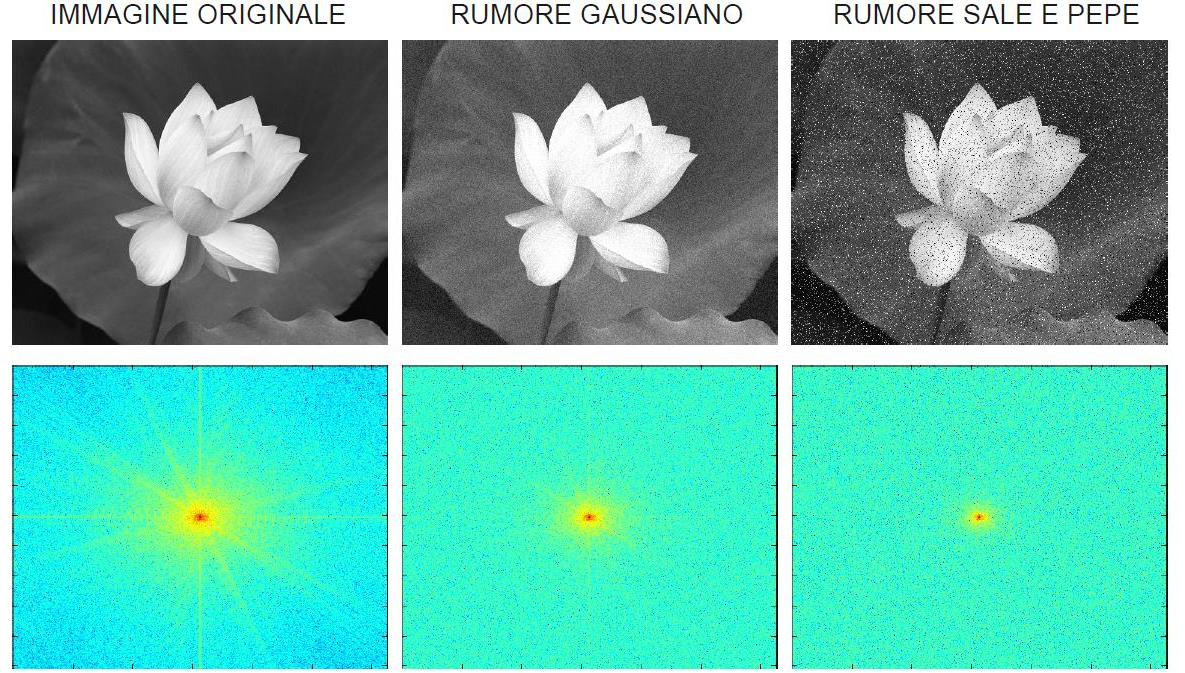
\includegraphics[width=\textwidth]{img/rumore_dominio_frequenze.jpg}
	\end{figure}\newpage

	\subsection{Panoramica su filtri passa alto (\emph{high-pass}) e passa basso (\emph{low-pass})}
	
	I filtri passo alto (\emph{high-pass}) e passa basso (\emph{low-pass}) sono identici a quelli visti durante il corso di Sistemi. L'obbiettivo di questo paragrafo è introdurre qualche definizione e dare una panoramica generale dei due filtri approfonditi nei prossimi paragrafi.\newline
	
	\noindent
	In un immagine, le \textbf{frequenze basse} rappresentano informazioni con variazioni di intensità \dquotes{lente}. Per esempio, le gradazioni di colore su un muro illuminato, o la nuvolosità nel cielo.\newline
	
	\noindent
	Al contrario, le informazioni ad \textbf{alte frequenze} indicano informazioni con variazioni di intensità \dquotes{repentine}. Per esempio, spigoli, angoli e rumore.\newline
	
	\noindent
	Per lavorare sulle frequenze esistono due filtri importanti:
	\begin{itemize}
		\item \textcolor{Red3}{\textbf{Filtro passa basso}} \emph{(low-pass filter)} rimuove dall'immagine le informazioni ad alte frequenze e mantiene quelle a basse frequenze.
		
		\item \textcolor{Red3}{\textbf{Filtro passa alto}} \emph{(high-pass filter)} rimuove dall'immagine le informazioni a basse frequenze e mantiene quelle ad alte frequenze.
	\end{itemize}
	Dato che ogni filtro è il contrario dell'altro, da ciascuno è possibile derivare il suo opposto:
	\begin{equation*}
		H_{PA} = 1 - H_{PB}
	\end{equation*}
	In cui $PA$ indica passa alto e $PB$ passa basso.\newpage
	
	\subsection{Filtri passa basso (\emph{low-pass})}
	
	\subsubsection{Filtri passa basso ideale}
	
	Il \textcolor{Red3}{\textbf{filtro passa basso ideale}} viene usato per ottenere: lo sfocamento e lo \emph{smoothing}. Solitamente, per ottenere questi risultati si attenuano le alte frequenze, ma facendo così si ottiene anche una riduzione inevitabile del rumore.\newline
	
	\noindent
	Matematicamente parlando, un filtro passa basso ideale è una funzione di trasferimento (uguale alla sua trasformata nel dominio delle frequenze) di una box.\newline
	
	\noindent
	Viene detta \textbf{ideale} perché come si vede in figura, una transizione così netta in corrispondenza alla \emph{frequenza di taglio} non è analogicamente realizzabile. In parole povere, è ideale poiché nell'elettronica non può fisicamente avvenire un calo di energia così repentino.
	\begin{figure}[!htp]
		\centering
		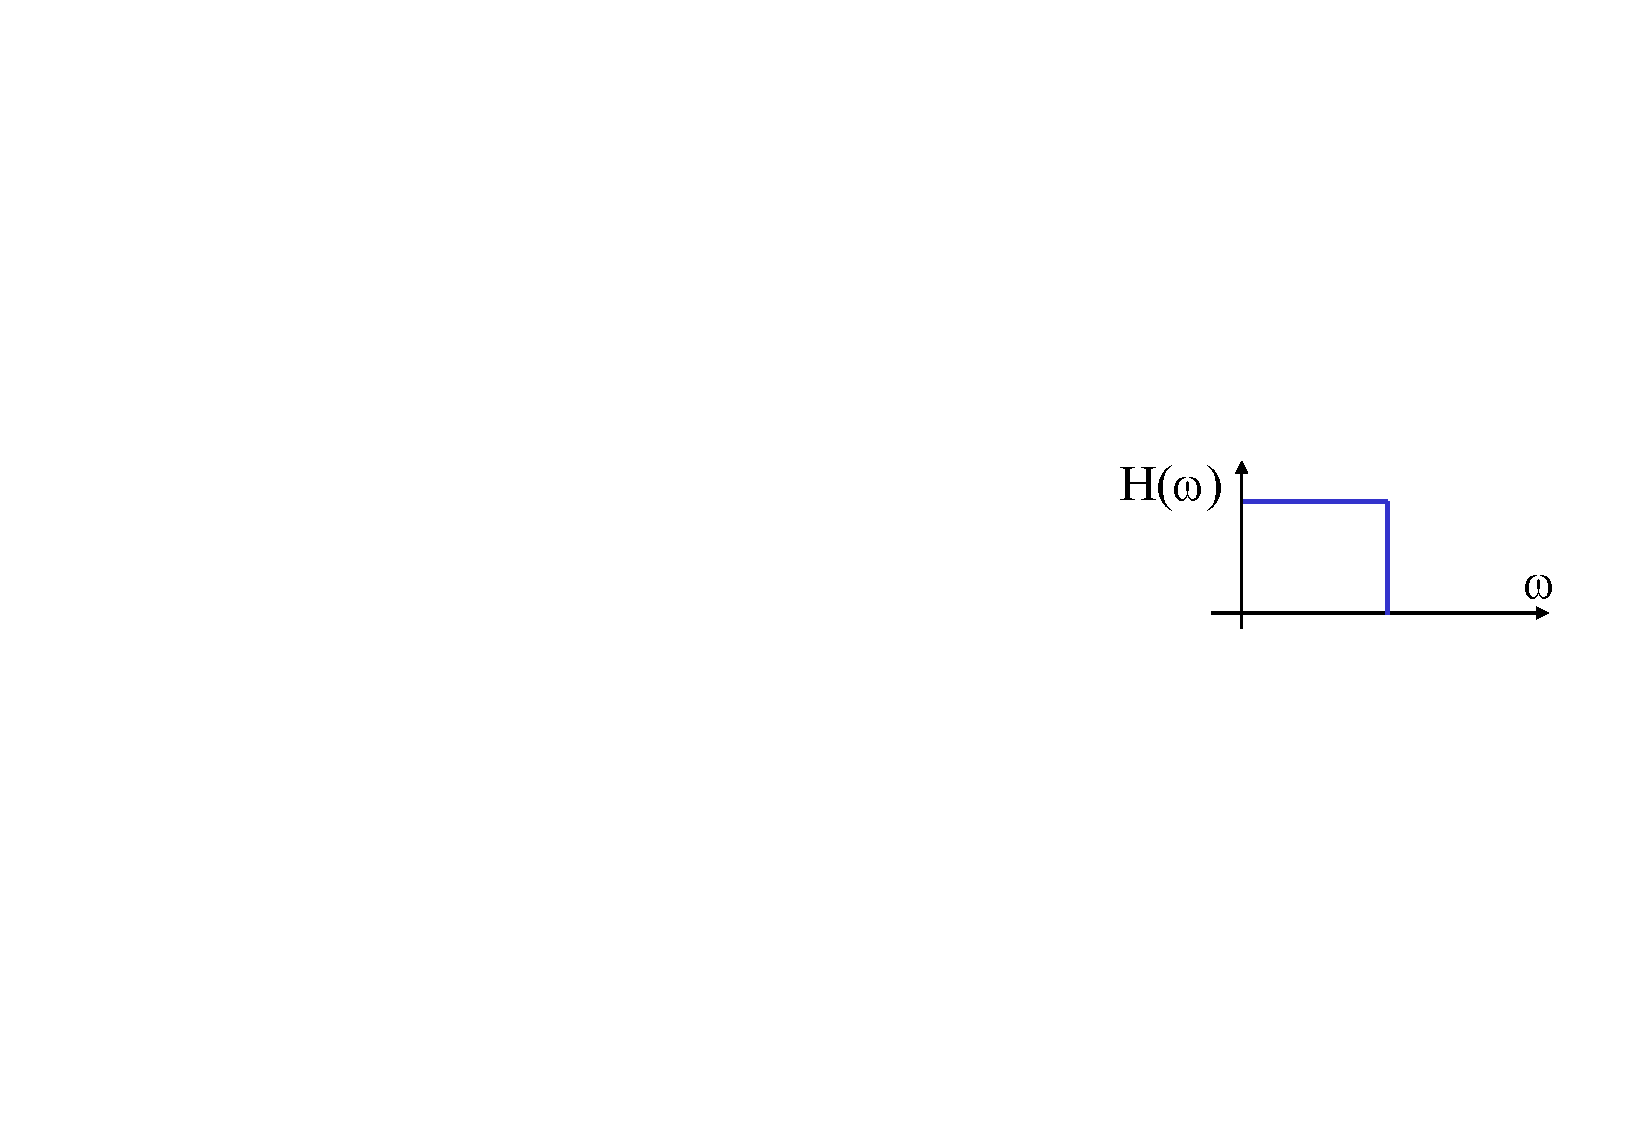
\includegraphics[width=.4\textwidth]{img/box_filtro_passa_bassa_ideale.pdf}
		\caption{Funzione di trasferimento di un filtro passa basso ideale.}
	\end{figure}

	\noindent
	Dato che i filtri studiati sono solamente digitali, teoricamente potremmo tralasciare questo taglio repentino. Purtroppo, esso provoca un effetto visivo indesiderato chiamato \textbf{ringing}.\newline
	
	\noindent
	Il \textcolor{Red3}{\textbf{ringing}} (o effetto di Gibbs) è dovuto al fatto eseguire un filtraggio passa basso ideale (in frequenza) equivale ad eseguire una convoluzione con l'operatore $\mathrm{sinc}$ (nello spazio). Ne consegue che la risposta all'impulso del passa basso ideale è ancora un $\mathrm{sinc}$ e l'\textbf{immagine visivamente risulta increspata vicino ai bordi taglienti}\footnote{Fonte: \href{https://imaging.cs.msu.ru/en/research/ringing}{\emph{Faculty of Computational Mathematics and Cybernetics, Lomonosov Moscow State University}}}.
	\begin{figure}[!htp]
		\centering
		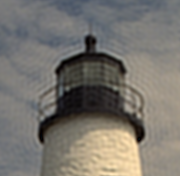
\includegraphics[width=.4\textwidth]{img/ringing_example.png}
		\caption{Effetto ringing su un'immagine.}
	\end{figure}\newpage

	\noindent
	Segnale $H$:
	\begin{figure}[!htp]
		\centering
		\includegraphics[width=.3\textwidth]{img/filtro_passa_basso_ideale.pdf}
	\end{figure}

	\noindent
	Le formule da applicare per il filtro basso ideale sono:
	\begin{equation*}
		H\left(u,v\right) = \begin{cases}
			1 & \text{se } D\left(u,v\right) \le D_{0} \\
			0 & \text{se } D\left(u,v\right) > D_{0}
		\end{cases}
	\end{equation*}
	In cui $D_{0}$ è uguale a $\mu_{\text{thresh}}$ che indica la soglia e $D\left(u,v\right)$ è il raggio del cerchio:
	\begin{equation*}
		D\left(u,v\right) = \sqrt{\left(u - \dfrac{M}{2}\right)^{2} + \left(v - \dfrac{N}{2}\right)^{2}}
	\end{equation*}
	Da notare che solo le frequenze nel cerchio di raggio $D_{0}$ vengono mantenute.\newpage
	
	\subsubsection{Filtri passa basso di Butterworth}
	
	Il \textcolor{Red3}{\textbf{filtro passa basso di Butterworth}} è un filtro con attenuazione dolce in prossimità della frequenza di taglio.	
	\begin{figure}[!htp]
		\centering
		\includegraphics[width=.9\textwidth]{img/filtro_passa_basso_butterworth.png}
		\caption{Filtro passa basso di Butterworth.}
	\end{figure}
	La \textbf{proprietà caratterizzante} di questo filtro è la \textbf{risposta molto ripida nella banda passante}.\newline
	
	\noindent
	L'ordine è $n$ e la frequenza di taglio $D_{0} = \mu_{\text{thresh}}$:
	\begin{equation*}
		H\left(u,v\right) = \dfrac{1}{1 + \left(\dfrac{D\left(u,v\right)}{D_{0}}\right)^{2n}}
	\end{equation*}

	\begin{figure}[!htp]
		\centering
		\includegraphics[width=\textwidth]{img/filtro_passa_basso_butterworth-ordine.png}
		\caption{Applicazione dell'ordine e della frequenza di taglio.}
	\end{figure}

	\noindent
	Le formule da applicare:
	\begin{equation*}
		\begin{array}{lll}
			H\left(u,v\right) & = & \dfrac{1}{1 + \left[\dfrac{D\left(u,v\right)}{D_{0}}\right]^{2n}} \\
			&& \\
			D\left(u,v\right) & = & \sqrt{\left(u - \dfrac{M}{2}\right)^{2} + \left(v - \dfrac{N}{2}\right)^{2}}
		\end{array}
	\end{equation*}
	
	\noindent
	È interessante notare che facendo tendere $n$ all'infinito, si ottiene il filtro passa basso ideale:
	\begin{figure}[!htp]
		\centering
		\includegraphics[width=\textwidth]{img/filtro_passa_basso_butterworth-ideale.png}
	\end{figure}\newpage

	\subsubsection{Filtri passa basso Gaussiano}
	
	La trasformata di Fourier di una funzione Gaussiana è anch'essa Gaussiana:
	\begin{equation*}
		\begin{array}{lll}
			F\left(u\right) & = & Ae^{-\frac{u}{2\sigma^{2}}} \\
			&& \\
			f\left(t\right) & = & \sqrt{2 \pi} \sigma A e^{-2 \pi^{2} \sigma^{2} t^{2}}
		\end{array}
	\end{equation*}
	Oppure allo stesso identico modo:
	\begin{equation*}
		\begin{array}{lll}
			f\left(t\right) & = & Ae^{-\frac{t}{2\sigma^{2}}} \\
			&& \\
			F\left(u\right) & = & \sqrt{2 \pi} \sigma A e^{-2 \pi^{2} \sigma^{2} u^{2}}
		\end{array}
	\end{equation*}
	Le equazioni di questa operazione sono:
	\begin{equation*}
		\begin{array}{lll}
			H\left(u,v\right) & = & e^{-\dfrac{D^{2}\left(u,v\right)}{2 D_{0}^{2}}} \\
			&& \\
			D\left(u,v\right) & = & \sqrt{\left(u - \dfrac{M}{2}\right)^{2} + \left(v - \dfrac{N}{2}\right)^{2}}
		\end{array}
	\end{equation*}
	In cui la costante $D_{0}$ può essere sostituita con $\sigma$, ovvero l'effettiva deviazione standard della distribuzione Gaussiana. In questo caso, la frequenza di taglio $D_{0}$ corrisponde alla deviazione standard $\sigma$. In altre parole, quando $D\left(u,v\right) = \sigma$, allora l'intensità di taglio è $0.607$ e il filtraggio crea un attenuamento di quella frequenza pari al $60.7\%$.\newline
	
	\noindent
	Un'\textbf{osservazione} interessante è la seguente. Un filtro gaussiano con una certa scala nel dominio delle frequenze, corrisponde ad un filtro gaussiano con scala inversa nel dominio dello spazio.
	
	\subsubsection{Sintesi}
	
	Qui di seguito si elencano i filtri passa basso più importanti:
	\begin{itemize}
		\item \textbf{Ideale}: è una brusca transizione in corrispondenza della frequenza di \emph{cut-off}. Questo causa un fenomeno di Gibbs o di \emph{ringing};
		
		\item \textbf{Gaussiano}: transizione di \emph{cut-off} dolce. Il parametro $\sigma$ determina la frequenza di \emph{cut-off};
		
		\item \textbf{Butterworth}: ha una rapidità variabile e transizione \emph{smooth}. La ripidità viene modellata dall'ordine del filtro. La frequenza di \emph{cut-off} viene selezionata indipendentemente dall'ordine del filtro. Si può avere \emph{ringing} per ordini elevati.
	\end{itemize}\newpage
	
	\subsection{Filtri passa alto (\emph{high-pass})}
	
	Un \textcolor{Red3}{\textbf{filtro passa alto}} sopprime (blocca) le basse frequenze e lascia passare le alte frequenze. La costruzione di un filtro passa alto può essere eseguita come:
	\begin{equation*}
		H_{PA} = 1 - H_{PB}
	\end{equation*}
	\begin{figure}[!htp]
		\centering
		\includegraphics[width=.9\textwidth]{img/filtri_passa_alto.png}
		\caption{Filtri passa alto, dall'alto: ideale, di Butterworth, Gaussiano.}
	\end{figure}\newpage
	
	\subsubsection{Filtri passa alto ideale}
	
	Dato il segnale $H$:
	\begin{figure}[!htp]
		\centering
		\includegraphics[width=.3\textwidth]{img/filtro_passa_alto_ideale.pdf}
	\end{figure}
	
	\noindent
	Le formule da applicare per il \textcolor{Red3}{\textbf{filtro passa alto ideale}} sono:
	\begin{equation*}
		\begin{array}{lll}
			H\left(u,v\right) & = & \begin{cases}
				0 & \text{se} D\left(u,v\right) \le D_{0} \\
				1 & \text{se} D\left(u,v\right) > D_{0}
			\end{cases} \\
			&& \\
			D\left(u,v\right) & = & \sqrt{\left(u - \dfrac{M}{2}\right)^{2} + \left(v - \dfrac{N}{2}\right)^{2}}
		\end{array}
	\end{equation*}
	Solamente le frequenze fuori dal cerchio di raggio $D_{0}$ vengono mantenute.
	
	\subsubsection{Filtri passa alto di Butterworth}
	
	Dato il segnale $H$:
	\begin{figure}[!htp]
		\centering
		\includegraphics[width=.3\textwidth]{img/filtro_passa_alto_butterworth.png}
	\end{figure}
	
	\noindent
	Le formule da applicare per il \textcolor{Red3}{\textbf{filtro passa alto di Butterworth}} sono:
	\begin{equation*}
		\begin{array}{lll}
			H\left(u,v\right) & = & \dfrac{1}{1 + \left[\dfrac{D\left(u,v\right)}{D_{0}}\right]^{-2n}} \\
			&& \\
			D\left(u,v\right) & = & \sqrt{\left(u - \dfrac{M}{2}\right)^{2} + \left(v - \dfrac{N}{2}\right)^{2}}
		\end{array}
	\end{equation*}
	Per $n$ tendente ad infinito si ha il filtro passa alto ideale.\newpage
	
	\subsubsection{Filtri passa alto Gaussiano}
	
	Dato il segnale $H$:
	\begin{figure}[!htp]
		\centering
		\includegraphics[width=.3\textwidth]{img/filtro_passa_alto_gaussiano.png}
	\end{figure}
	
	\noindent
	Le formule da applicare per il \textcolor{Red3}{\textbf{filtro passa alto Gaussiano}} sono:
	\begin{equation*}
		\begin{array}{lll}
			H\left(u,v\right) & = & 1 - e^{- \dfrac{D^{2}\left(u,v\right)}{2 D^{2}_{0}}} \\
			&& \\
			D\left(u,v\right) & = & \sqrt{\left(u - \dfrac{M}{2}\right)^{2} + \left(v - \dfrac{N}{2}\right)^{2}}
		\end{array}
	\end{equation*}\newpage

	\subsection{Filtri per enfatizzare le alte frequenze}
	
	Esiste anche il \textcolor{Red3}{\textbf{filtro omeomorfo}} che attenua le basse frequenze e aumenta quelle delle alte:
	\begin{equation*}
		H\left(u,v\right) = \left(\gamma_{H} - \gamma_{L}\right)\left[1 - e^{- \frac{c D^{2}\left[u,v\right]}{D_{0}^{2}}}\right] + \gamma_{L}
	\end{equation*}

	\noindent
	Invece, usando il \textbf{filtro passa alto}, è possibile enfatizza aumentando la variabile $k$:
	\begin{equation*}
		H\left(u,v\right) = \left(1 + k \cdot H_{PA}\left(u,v\right)\right) \cdot H
	\end{equation*}
	Dove $k$ è il contributo delle alte frequenze, $H$ lo spettro dell'immagine e $H_{PA}$ il filtro passa alto\newpage
	
	\subsection{Filtri passa banda ideale 1D e ferma banda ideale}
	
	I seguenti filtri operano su una banda di frequenze, al contrario i precedenti filtri lavoravano su alte o basse frequenze.\newline
	
	\noindent
	Analogamente ai filtri passa basso e alto, anche qui è possibile derivare uno dei due filtri avendo solamente l'altro:
	\begin{equation*}
		H_{PBn} = 1 - H_{FBn}
	\end{equation*}
	Dove $PB$ indica passa banda e $FB$ ferma banda.\newline
	
	\noindent
	Un \textcolor{Red3}{\textbf{filtro passa banda ideale 1D}} sopprime tutte le frequenze al di fuori di un intervallo di frequenze specificato. Più formalmente, esso è rappresentato con la seguente funzione:
	\begin{equation*}
		G\left(\mu\right) = \begin{cases}
			1	& \text{se } u_{1} < \left|u\right| < u_{2} \\
			0	& \text{altrimenti}
		\end{cases}
	\end{equation*}
	Le variabili $u$ rappresentano l'intervallo (come si vede in figura) e al di fuori di esso il valore è zero.
	\begin{figure}[!htp]
		\centering
		\includegraphics[width=.5\textwidth]{img/filtro_passa_banda_ideale.pdf}
		\caption{Rappresentazione grafica del filtro passa banda ideale 1D nel \textbf{dominio delle frequenze}.}
	\end{figure}
	
	\noindent
	Dalla rappresentazione grafica si ricava anche la relativa \textbf{funzione di trasferimento nel dominio delle \underline{frequenze}}, ovvero la somma di due box traslate nel tempo ottenibili eseguendo la convoluzione di una box per due impulsi unitari (Dirac):
	\begin{equation*}
		G\left(u\right) = \Pi\left(\dfrac{u}{\Delta u}\right) * \left[\delta\left(u-u_{0}\right) + \delta\left(u+u_{0}\right)\right]
	\end{equation*}
	Dove i termini $u_{0}$ e $\Delta u$ indicano:
	\begin{itemize}
		\item $u_{0}$ indica dov'è centrata la box ed è ottenibile in questo modo:
		\begin{equation*}
			u_{0} = \dfrac{\left(u_{1} + u_{2}\right)}{2}
		\end{equation*}
		
		\item $\Delta u$ indica la larghezza della box ed è ottenibile in questo modo:
		\begin{equation*}
			\Delta u = u_{2} - u_{1}
		\end{equation*}
	\end{itemize}\newpage
	
	\noindent
	Invece, la \textbf{funzione di trasferimento nel dominio del \underline{tempo}} è la seguente:
	\begin{equation*}
		g\left(t\right) = 2\Delta u \cdot \dfrac{\sin\left(\pi t \Delta u\right)}{\pi t \Delta u} \cdot \cos\left(2 \pi u_{0} t\right)
	\end{equation*}
	Dato che $\Delta u < u_{0}$, allora la funzione $g\left(t\right)$ è un coseno modulato dal $\mathrm{sinc}$. Pensandoci bene, la box viene rappresentata dalla funzione $\mathrm{sinc}$\footnote{Si ricorda che la funzione $\mathrm{sinc}$ è così formata: $\mathrm{sinc}\left(x\right) = \dfrac{\sin\left(\pi x\right)}{\pi x}$} e i due impulsi possono essere rappresentati, ricordando il corso di sistemi, dalla funzione coseno. Se $u_{0}$ è costante e $\Delta u_{0}$ tende a zero, allora si ha un coseno.
	
	\begin{figure}[!htp]
		\centering
		\includegraphics[width=.7\textwidth]{img/filtro_passa_banda_ideale_grafico_tempo.pdf}
		\caption{Rappresentazione grafica del filtro passa banda ideale 1D nel \textbf{dominio del tempo}.}
	\end{figure}\newpage
	
	\noindent
	Un \textcolor{Red3}{\textbf{filtro ferma banda ideale}} sopprime tutte le frequenze nell'intervallo specificato. Più formalmente, esso è rappresentato con la seguente funzione:
	\begin{equation*}
		G\left(\mu\right) = \begin{cases}
			0	& \text{se } u_{1} < \left|u\right| < u_{2} \\
			1	& \text{altrimenti}
		\end{cases}
	\end{equation*}
	Le variabili $u$ rappresentano l'intervallo (come si vede in figura) e al di fuori di esso il valore è uno. Quindi, al contrario del filtro passa banda ideale, il ferma banda non consente al segnale di esistere nelle frequenze specificate.
	\begin{figure}[!htp]
		\centering
		\includegraphics[width=.5\textwidth]{img/filtro_ferma_banda_ideale.pdf}
		\caption{Rappresentazione grafica del filtro ferma banda ideale nel \textbf{dominio delle frequenze}.}
	\end{figure}

	\noindent
	Dalla rappresentazione grafica si ricava anche la relativa \textbf{funzione di trasferimento nel dominio delle \underline{frequenze}}, ovvero la rimozione (segno meno) di due box traslate nel tempo ottenibili eseguendo la convoluzione di una box per due impulsi unitari (Dirac):
	\begin{equation*}
		G\left(u\right) = 1 - \Pi\left(\dfrac{u}{\Delta u}\right) * \left[\delta\left(u-u_{0}\right) + \delta\left(u+u_{0}\right)\right]
	\end{equation*}
	I valori $u_{0}, \Delta u$ hanno lo stesso significato del filtro passa banda ideale. Invece, la \textbf{funzione di trasferimento nel dominio del \underline{tempo}} è la seguente:
	\begin{equation*}
		g\left(t\right) = \delta\left(t\right) - 2\Delta u \cdot \dfrac{\sin\left(\pi t \Delta u\right)}{\pi t \Delta u} \cdot \cos\left(2 \pi u_{0} t\right)
	\end{equation*}
	\begin{figure}[!htp]
		\centering
		\includegraphics[width=.5\textwidth]{img/filtro_ferma_banda_ideale_grafico_tempo.pdf}
		\caption{Rappresentazione grafica del filtro ferma banda ideale nel \textbf{dominio del tempo}.}
	\end{figure}\newpage
	
	\section{Elaborazione di immagini - Estrazione di edge robusta}
	
	\subsection{Estrazione di contorni (\emph{edge})}
	
	Si definisce come \textbf{\emph{feature}} una proprietà dell'immagine. Quest'ultima può essere:
	\begin{itemize}
		\item \textbf{Globale}, ovvero dell'intera immagine;
		\item \textbf{Locale}, ovvero di una parte dell'immagine con speciali proprietà.
	\end{itemize}
	
	\noindent
	Con il termine \textcolor{Red3}{\textbf{edge}} si indica una forte variazione locale dei livelli di grigio, tipicamente associata ad un contorno o ad una separazione tra regioni.\newline
	
	\noindent
	Il fenomeno dell'\emph{edge} provoca una serie di complicazioni. Si definisce il \textcolor{Red3}{\textbf{problema dell'estrazione}}: data un'immagine, la \textbf{rilevazione} (\emph{detection}) e la \textbf{localizzazione} degli edge derivati dalla scena e non dal rumore.\newline
	
	\noindent
	La soluzione al problema non è affatto banale perché: il rumore può mascherare gli \emph{edge} e possono esistere falsi \emph{edge} positivi dovuti a ombre e variazioni di luminosità.\newline
	
	\noindent
	Esistono varie \textbf{tipologie di livello di grigio}:
	\begin{figure}[!htp]
		\centering
		\includegraphics[width=\textwidth]{img/tipologie_ldg.pdf}
	\end{figure}

	\longline\vspace{1em}
	
	\noindent
	Si definisce un \textcolor{Red3}{\textbf{punto di edge}}, un punto dell'immagine con coordinate $\left(i,j\right)$ in cui è presente una variazione significativa locale dell'intensità.\newline
	
	\noindent
	Si definisce un \textcolor{Red3}{\textbf{contorno}}, una lista di punti di \emph{edge} o un'altra struttura dati che modella i punti di \emph{edge}, ordinandoli dal primo all'ultimo. In altre parole, è l'\emph{edge} vero e proprio.\newline
	
	\noindent
	Ancora una volta, nasce una complicazione: il \textcolor{Red3}{\textbf{problema della localizzazione}}. Infatti, nonostante la posizione di un punto di \emph{edge} si identifica tramite le coordinate $\left(i,j\right)$, le costanti $i,j$ potrebbero non essere indici di pixel.\newline
	
	\noindent
	Inoltre, la localizzazione può richiedere anche l'\textbf{orientazione} di un punto d'\emph{edge}. Questo implica l'introduzione del \textbf{gradiente}.\newline
	
	\longline\vspace{1em}
	
	\noindent
	Per concludere, si \textbf{classificano gli \emph{edge}}:
	\begin{itemize}
		\item \textbf{Corretti}: \emph{edge} della scena;
		\item \textbf{Falsi}: non esistono nella scena (\emph{false positives});
		\item \textbf{Mancanti}: presenti nella scena, ma non rilevanti (\emph{false negatives}).
	\end{itemize}\newpage

	\subsection{Criteri per \emph{edge detector} ottimi}
	
	Esistono $3$ criteri per ottenere un \emph{edge detector} ottimo:
	\begin{itemize}
		\item \textcolor{Red3}{\textbf{Buon rilevamento (\emph{detection})}}. Deve minimizzare la probabilità di presenza di falsi positivi e la probabilità di presenza di falsi negativi.\newline
		La massimizzazione del SNR (\emph{Signal to Noise Ratio}, rapporto segnale-rumore; è una grandezza numerica che mette in relazione la potenza del segnale utile rispetto a quella del rumore\footnote{Fonte: \href{https://it.wikipedia.org/wiki/Rapporto_segnale/rumore}{WikipediaIT}}) definito come il rapporto tra la risposta quadratica media (RMS) del filtro agli \emph{step edge} ideali e il rumore;
		
		\item \textcolor{Red3}{\textbf{Buona localizzazione}}. Gli \emph{edge} rilevati devono essere più vicino possibile agli \emph{edge} reali;
		
		\item \textcolor{Red3}{\textbf{Vincolo di singola risposta}}. Per ogni punto di \emph{edge} reale, il filtro deve rilevare \underline{un solo} punto di \emph{edge}. Ossia, minimizzare il numero di massimi locali creati dal rumore intorno all'\emph{edge}.
	\end{itemize}
	I criteri di buon rilevamento e di buona localizzazione, identificano due modi di valutazione per l'estrazione di \emph{edge} indipendentemente dalla lunghezza dell'\emph{edge} e dalla potenza del rumore.\newpage
	
	\subsection{Il gradiente}
	
	Il \textcolor{Red3}{\textbf{gradiente}} è una misura della variazione in una funzione. Nel caso monodimensionale, corrisponde al picco della derivata prima:
	\begin{figure}[!htp]
		\centering
		\includegraphics[width=\textwidth]{img/gradiente.pdf}
	\end{figure}
	
	\noindent
	Assumendo una funzione $f\left(x,y\right)$, allora:
	\begin{equation*}
		\boldsymbol{G}\left[f\left(x,y\right)\right] = \begin{bmatrix}
			G_{x} \\
			G_{y}
		\end{bmatrix} = \begin{bmatrix}
		\dfrac{\partial f}{\partial x} \\
		\\
		\dfrac{\partial f}{\partial y}
	\end{bmatrix}
	\end{equation*}
	Il modulo è pari alla lunghezza del vettore $G$ localizzato su $x$ e $y$:
	\begin{equation*}
		\left\| \boldsymbol{G} \right\| = G = \sqrt{G_{x}^{2} + G_{y}^{2}}
	\end{equation*}
	Approssimazioni del modulo:
	\begin{equation*}
		\begin{array}{lll}
			G & \cong & \left| G_{x} \right| + \left| G_{y} \right| \\
			G & \cong & \max\left(\left| G_{x} \right|, \left| G_{y} \right|\right)
		\end{array}	
	\end{equation*}
	L'orientazione, misurata rispetto all'asse $x$, è data da:
	\begin{equation*}
		\alpha\left(x,y\right) = \arctan\dfrac{G_{y}}{G_{x}}
	\end{equation*}
	In pratica, il vettore $\boldsymbol{G}$ punta nella direzione di massimo scarto della funzione $f$:
	\begin{figure}[!htp]
		\centering
		\includegraphics[width=.3\textwidth]{img/gradiente_direzione.pdf}
	\end{figure}\newpage
	
	\subsection{Estrazione dell'\emph{edge}}
	
	\subsubsection{Il gradiente discreto}
	
	Per differenziare un'immagine digitale $F\left[x,y\right]$ è possibile seguire due strade:
	\begin{enumerate}
		\item Ricostruire un'immagine continua, quindi prendere il gradiente analitico;
		\item Prendere la derivata discreta, tramite \dquotes{differenze finite}, come visto nei capitoli precedenti.
	\end{enumerate}
	Il \textbf{gradiente discreto} è approssimativamente la differenza tra pixel adiacenti:
	\begin{equation*}
		\dfrac{\partial f}{\partial x}\left[x,y\right] \approx F\left[x + 1, y\right] - F\left[x,y\right]
	\end{equation*}
	E le approssimazioni numeriche, invece, sono:
	\begin{equation*}
		\begin{array}{lllll}
			f_{x} & \approx & f\left[i, j+1\right] - f\left[i,j\right] \longrightarrow \begin{bmatrix}
				-1 & 1
			\end{bmatrix} & \longrightarrow & S_{x} = \begin{bmatrix}
			-1 & 1 \\
			0 & 0
		\end{bmatrix} \\
			f_{y} & \approx & f\left[i,j\right] - f\left[i+1, j\right] \longrightarrow \begin{bmatrix}
				1 \\
				-1
			\end{bmatrix} & \longrightarrow & S_{y} = \begin{bmatrix}
			1 & 0 \\
			-1 & 0
		\end{bmatrix}
		\end{array}
	\end{equation*}\label{gradiente discreto}

	\longline
	
	\subsubsection{Operatore di Roberts}
	
	L'\textcolor{Red3}{\textbf{operatore di Roberts}} è un'approssimazione con differenze incrociate:
	\begin{equation*}
		\left|d\left[f\left(i,j\right)\right]\right| = \left|f\left(i,j\right) - f\left(i+1, j+1\right)\right| + \left|f\left(i, j+1\right) - f\left(i+1, j\right)\right|
	\end{equation*}
	La convoluzione dell'immagine (guardare le due matrici $S_{x}$ e $S_{y}$ nel paragrafo~\ref{gradiente discreto}) con $2$ maschere del tipo:
	\begin{equation*}
		S_{1} = \begin{bmatrix}
			1 & 0 \\
			0 & -1
		\end{bmatrix} \hspace{2em} S_{2} = \begin{bmatrix}
			0 & 1 \\
			-1 & 0
	\end{bmatrix}
	\end{equation*}

	\longline
	
	\subsubsection{Operatore di Prewitt}
	
	Data l'approssimazione con vicinato $3\times3$:
	\begin{equation*}
		\begin{bmatrix}
			a_{0} & a_{1} & a_{2} \\
			a_{7} & \left(i,j\right) & a_{3} \\
			a_{6} & a_{5} & a_{4}
		\end{bmatrix}
	\end{equation*}
	L'\textcolor{Red3}{\textbf{operatore di Prewitt}} è un'approssimazione del tipo:
	\begin{equation*}
		\left|r\left[f\left(i,j\right)\right]\right| = \underbrace{\left|\left(a_{2}+a_{3}+a_{4}\right) - \left(a_{0}+a_{7}+a_{6}\right)\right|}_{S_{x}} + \underbrace{\left|\left(a_{0}+a_{1}+a_{2}\right) - \left(a_{6}+a_{5}+a_{4}\right)\right|}_{S_{y}}
	\end{equation*}
	Il risultato:
	\begin{equation*}
		S_{x} = \begin{bmatrix}
			-1 & 0 & 1 \\
			-1 & 0 & 1 \\
			-1 & 0 & 1
		\end{bmatrix} \hspace{2em}
		S_{y} = \begin{bmatrix}
			1  & 1  & 1 \\
			0  & 0  & 0 \\
			-1 & -1 & -1
		\end{bmatrix}
	\end{equation*}\newpage
	
	\subsubsection{Operatore di Sobel}
	
	L'\textcolor{Red3}{\textbf{operatore di Sobel}} ha molte matrici predefinite, tra le più famose:
	\begin{equation*}
		S_{x} = \begin{bmatrix}
			-1 & 0 & 1 \\
			-2 & 0 & 2 \\
			-1 & 0 & 1
		\end{bmatrix} \hspace{2em}
		S_{y} = \begin{bmatrix}
			1  & 2  & 1 \\
			0  & 0  & 0 \\
			-1 & -2 & -1
		\end{bmatrix}
	\end{equation*}
	
	\longline
	
	\subsubsection{Operatore di Kirsch}
	
	L'\textcolor{Red3}{\textbf{operatore di Roberts}} ha $8$ maschere direzionali, ognuna delle quali risponde massimamente per ciascun \emph{edge} in una determinata direzione. Il \textbf{valore massimo} tra gli $8$ valori stimati è il valore di output del gradiente in quel punto, mentre l'indice della maschera codifica le direzioni dell'\emph{edge}.\newline
	
	\noindent
	Un \textbf{esempio di maschere direzionali}:
	\begin{equation*}
		\begin{array}{lllc}
			\textbf{Horizontal line: } & D_{0} & = & \begin{bmatrix}
				-1 & -1  & -1 \\
				2 & 2 & 2 \\
				-1 & -1 & -1
			\end{bmatrix} \\
			&&& \\
			\boldsymbol{45°}\textbf{ line: } & D_{45} & = & \begin{bmatrix}
				-1 & -1  & 2 \\
				-1 & 2 & -1 \\
				2 & -1 & -1
			\end{bmatrix} \\
			&&& \\
			\textbf{Vertical line: } & D_{90} & = & \begin{bmatrix}
				-1 & 2  & -1 \\
				-1 & 2 & -1 \\
				-1 & 2 & -1
			\end{bmatrix} \\
			&&& \\
			\boldsymbol{135°}\textbf{ line: } & D_{135} & = & \begin{bmatrix}
				2 & -1  & -1 \\
				-1 & 2 & -1 \\
				-1 & -1 & 2
			\end{bmatrix} \\
		\end{array}
	\end{equation*}
	
	\longline
	
	\subsubsection{Operatore di Robinson}
	
	L'\textcolor{Red3}{\textbf{operatore di Roberts}} ha $8$ maschere direzionali, simili a quelle di Kirsch.\newpage
	
	\subsubsection{Confronto tra operatori}
	
	Dati gli operatori per estrarre l'\emph{edge}:
	\begin{enumerate}
		\item Gradiente
		\item Roberts
		\item Prewitt
		\item Sobel
	\end{enumerate}
	È possibile osservare come più si è \textbf{vicini al gradiente}, più:
	\begin{itemize}
		\item La localizzazione è buona;
		\item Aumenta la sensibilità al rumore;
		\item Diminuisce la rilevazione, diventa scarsa con il gradiente.
	\end{itemize}
	Al contrario, \textbf{vicino all'operazione di Sobel}:
	\begin{itemize}
		\item Diminuisce la localizzazione;
		\item Diminuisce la sensibilità al rumore;
		\item Aumenta la rilevazione.
	\end{itemize}
	Un esempio di applicazione dei vari operatori:
	\begin{figure}[!htp]
		\centering
		\includegraphics[width=.65\textwidth]{img/confronto_tra_operatori.pdf}
	\end{figure}\newpage
	
	\noindent
	Invece, l'applicazione del gradiente è visibile nella seguente figura. Interessante notare le singoli applicazioni, ovvero solo lungo $x$ o $y$:
	\begin{figure}[!htp]
		\centering
		\includegraphics[width=.8\textwidth]{img/gradiente_examples.png}
	\end{figure}\newpage

	\subsection{Derivata prima}
	
	\subsubsection{Problemi}
	
	Gli operatori di \textbf{derivata prima} vanno applicati per ottenere il gradiente. Tuttavia, presentano dei problemi poiché \textbf{estraggono troppi punti di \emph{edge}}.
	
	\longline
	
	\subsubsection{Effetti del rumore}
	
	Si consideri una singola riga o colonna dell'immagine. Si traccia l'intensità in funzione della posizione del segnale. Si può vedere come la \textbf{derivata prima amplifichi il rumore}:
	\begin{figure}[!htp]
		\centering
		\includegraphics[width=.8\textwidth]{img/derivata_prima.pdf}
	\end{figure}

	\noindent
	Per \textbf{risolvere} questo problema, si applica uno \textbf{\emph{smoothing} preliminare}.

	\longline
	
	\subsubsection{Rilevazione di \emph{edge} o \emph{detection} robusta}
	
	Per rilevare l'\emph{edge} o eseguire una detection robusta, si eseguono tre fasi fondamentali:
	\begin{itemize}
		\item \textbf{Filtraggio} (\emph{noise smoothing}): si vuole ridurre il rumore preservando gli \emph{edge} reali;
		
		\item \textbf{Rinforzo} (\emph{enhancement, sharpening}): facilita il rilevamento dell'\emph{edge}, evidenziando le variazioni locali;
		
		\item \textbf{Rilevamento} (\emph{detection}): decisione sulla presenza o meno dei punti di \emph{edge}.
	\end{itemize}
	Tuttavia, si tenga in considerazione che:
	\begin{itemize}[label=\ding{42}]
		\item Non tutti i punti aventi gradiente diverso da zero sono \emph{edge};
		\item È richiesto tipicamente una fase di sogliatura;
		\item È richiesto talvolta una fase di localizzazione a risoluzione \emph{subpixel} e una fase di assottigliamento (\emph{thinning})
	\end{itemize}\newpage

	\subsubsection{Teorema di convoluzione}
	
	Applicando il \textbf{teorema di convoluzione}:
	\begin{equation*}
		\dfrac{\partial}{\partial x}\left(h * f\right) = \left(\dfrac{\partial}{\partial x}\right) * f
	\end{equation*}
	In questo modo, si risparmia un'operazione di filtraggio. Esempio:
	\begin{figure}[!htp]
		\centering
		\includegraphics[width=\textwidth]{img/convoluzione_derivata_prima.pdf}
	\end{figure}\newpage

	\subsection{Derivata seconda}
	
	\subsubsection{Operatori di derivata seconda}
	
	Gli \textcolor{Red3}{\textbf{operatori di derivata seconda}} rilevano il punto di \emph{edge} mediante il passaggio per lo zero (\emph{zero crossing}) del valore calcolato, e per questo motivo sono \textbf{più precisi} (non necessitano di stabilire una soglia).
	\begin{figure}[!htp]
		\centering
		\includegraphics[width=\textwidth]{img/derivata_seconda.pdf}
	\end{figure}
	
	\noindent
	Nell'immagine è visibile l'applicazione delle varie derivate. Con la derivata prima si evidenzia la massima discontinuità tra i pixel antistanti, mentre con la derivata seconda c'è la massima variazone, ovvero il valore è prossimo allo zero.
	
	\longline
	
	\subsubsection{Operatore Laplaciano}
	
	L'\textcolor{Red3}{\textbf{operatore Laplaciano}} equivale alla derivata seconda in $2$ dimensioni:
	\begin{equation*}
		\nabla^{2} f = \dfrac{\partial^{2} f}{\partial x^{2}} + \dfrac{\partial^{2} f}{\partial y^{2}}
	\end{equation*}
	Approssimando con l'equazione alle differenze e centrando la stima nel pixel $\left(i,j\right)$ si ha:
	\begin{equation*}
		\begin{array}{lll}
			\dfrac{\partial^{2} f}{\partial x^{2}} & = & f\left(i, j+1\right) - 2f\left(i,j\right) + f\left(i,j-1\right) \\
			&& \\
			\dfrac{\partial^{2} f}{\partial y^{2}} & = & f\left(i+1, j\right) - 2f\left(i,j\right) + f\left(i-1,j\right)
		\end{array}
	\end{equation*}
	Combinando in un singolo operatore, si nota che è isotropico:
	\begin{equation*}
		\begin{array}{lll}
			\nabla^{2} & = & \begin{bmatrix}
				0 & 1 & 0 \\
				1 & -4 & 1 \\
				0 & 1 & 0
			\end{bmatrix} \\
			&& \\
			\nabla^{2} & = & \begin{bmatrix}
				1 & 4 & 1 \\
				4 & -20 & 4 \\
				1 & 4 & 1
			\end{bmatrix} \\
			&& \\
			\nabla^{2} & = & \begin{bmatrix}
				0 & -1 & 0 \\
				-1 & 4 & -1 \\
				0 & -1 & 0
			\end{bmatrix} \\
			&& \\
			\nabla^{2} & = & \begin{bmatrix}
				-1 & -1 & -1 \\
				-1 & 8 & -1 \\
				-1 & -1 & -1
			\end{bmatrix}
		\end{array}
	\end{equation*}\newpage

	\subsection{Laplaciano di Gaussiana}
	
	L'\textcolor{Red3}{\textbf{operatore Laplaciano  di Gaussiana}} consiste in un filtraggio Gaussiano e Laplaciano. \textbf{È il metodo migliore per estrarre gli \emph{edge}}. Con questo operatore si può osservare che:
	\begin{itemize}[label=-]
		\item Il filtro di \emph{smoothing} è Gaussiano;
		\item La fase di rinforzo è la derivata seconda, cioè Laplaciano;
		\item Il rilevamento è la fase di attraversamento per lo zero;
		\item La localizzazione è fatta mediante interpolazione lineare.
	\end{itemize}
	L'\textbf{applicazione} di questo filtro Gaussiano ha i seguenti fini:
	\begin{itemize}
		\item \textbf{Riduzione del rumore} per punti isolati e piccole configurazioni;
		\item \dquotes{\textbf{Addolcimento} degli \emph{step edge}};
		\item \dquotes{\textbf{Diffondere (\emph{blur}) gli edge}}.
	\end{itemize}
	Considerando:
	\begin{equation*}
		\dfrac{\partial^{2}}{\partial x^{2}}\left(h*f\right)
	\end{equation*}
	I grafici sono:
	\begin{figure}[!htp]
		\centering
		\includegraphics[width=\textwidth]{img/laplaciano_gaussiana.pdf}
	\end{figure}\newpage
	
	\noindent
	L'\textbf{operatore laplaciano} viene indicato con la lettera nabla al quadrato $\nabla^{2}$:
	\begin{equation*}
		\nabla^{2}f = \dfrac{\partial^{2} f}{\partial x^{2}} + \dfrac{\partial^{2}f}{\partial y^{2}}
	\end{equation*}
	Considerando \emph{edge} soltanto i punti in cui:
	\begin{itemize}
		\item Laplaciano passa per lo zero;
		\item Gradiente locale è massimo (maggiore di una soglia quindi).
	\end{itemize}
	Allora l'uscita dell'operatore Laplaciano di Guassiana è $h\left(x,y\right)$:
	\begin{equation*}
		h\left(x,y\right) = \nabla^{2}\left[g\left(x,y\right) * f\left(x,y\right)\right] = \left[\nabla^{2}g\left(x,y\right)\right] * f\left(x,y\right)
	\end{equation*}
	Dove:
	\begin{equation*}
		\nabla^{2}g\left(x,y\right) = \dfrac{x^{2}+y^{2}-2\sigma^{2}}{2\sigma^{4}} \cdot \exp\left[-\dfrac{x^{2}y^{2}}{2\sigma^{2}}\right]
	\end{equation*}
	Quest'ultimo viene chiamato \textbf{\emph{mexican hat}} poiché ha la forma di cappello messicano:
	\begin{figure}[!htp]
		\centering
		\includegraphics[width=.4\textwidth]{img/mexican_hat.pdf}
	\end{figure}
	
	\noindent
	Adesso, grazie all'introduzione di questo operatore, le due seguenti operazioni sono \textbf{equivalenti}:
	\begin{enumerate}
		\item Eseguire la convoluzione dell'immagine con un filtro Gaussiano di \emph{smoothing} e calcolare il Laplaciano del risultato;
		\item Eseguire la convoluzione dell'immagine con un filtro lineare, ovvero il filtro Laplaciano di Guassiana.
	\end{enumerate}
	Si introduce un \textbf{esempio} di maschera $5\times5$:
	\begin{equation*}
		\begin{bmatrix}
			\phantom{-}0 & \phantom{-}0 & -1 & \phantom{-}0 & \phantom{-}0 \\
			\phantom{-}0 & -1 			& -2 & -1 			& \phantom{-}0 \\
			-1 			 & -2 			& 16 & -2 			& -1 \\
			\phantom{-}0 & -1 			& -2 & -1 			& \phantom{-}0 \\
			\phantom{-}0 & \phantom{-}0 & -1 & \phantom{-}0 & \phantom{-}0
		\end{bmatrix}
	\end{equation*}\newpage

	\noindent
	Data la formula del filtro, con diversi valori della varianza $\sigma$, si ottengono diversi risultati:
	\begin{itemize}
		\item $\boldsymbol{\sigma}$ \textbf{grande}:
		\begin{itemize}
			\item[\ding{51}] Riduzione del rumore migliore;
			\item[\ding{55}] Perdita notevole di informazioni utili
			\item[\ding{61}] Esempi: fusione di edge vicini, presenza di edge falsi, localizzazione imprecisa
		\end{itemize}
	
		\item $\boldsymbol{\sigma}$ \textbf{piccolo}:
		\begin{itemize}
			\item[\ding{51}] Riduzione del rumore minore;
			\item[\ding{55}] Riduzione di perdita di informazioni utili
			\item[\ding{61}] Esempio: molti edge spuri
		\end{itemize}
	\end{itemize}
	Per attenuare i difetti e cercare di ottenere un risultato ottimale, una \textbf{soluzione} comune è il \textbf{filtraggio a diversa scala} (diverse varianze):
	\begin{itemize}
		\item $\boldsymbol{\sigma}$ \textbf{grande}: pochi edge robusti, ma mal localizzati;
		\item $\boldsymbol{\sigma}$ \textbf{piccolo}: miglior localizzazione degli edge robusti.
	\end{itemize}
	Al \textbf{termine di un'applicazione di filtro Laplaciano di Gaussiana}, è necessario fondere i risultati delle varie scale ottenute, secondo alcuni criteri. Per esempio:
	\begin{itemize}
		\item Se ci sono \emph{edge} in tutte le scale;
		\item Se ci sono \emph{edge} almeno su $K$ scale;
		\item E così via.
	\end{itemize}
	L'esempio nella prossima pagina, dovrebbe chiarire maggiormente la teoria di questo filtro:
	\begin{figure}[!htp]
		\centering
		\includegraphics[width=\textwidth]{img/filtro_laplaciano_gaussiana.png}
	\end{figure}\newpage
	
	\subsection{Gradiente e Laplaciano di Gaussiana a confronto}
	
	L'operatore \textbf{gradiente} è efficace nel caso di immagini con poco rumore e transizioni nette.\newline
	
	\noindent
	Al contrario, l'operatore \textbf{Laplaciano di Gaussiana}, insieme allo \emph{zero crossing}, offre un'alternativa quando il rumore è elevato e le transizioni non sono nette.\newline
	Infatti, lo \emph{zero crossing} viene aggiunto poiché offre un modo affidabile per localizzare l'edge. Mentre le proprietà di \emph{smoothing} del Laplaciano di Gaussiana riducono gli effetti del rumore.\newpage
	
	\subsection{Filtro di Canny}
	
	\subsubsection{Definizione}
	
	Il \textcolor{Red3}{\textbf{filtro di Canny}} è uno degli strumenti più efficienti. È il contrapposto all'operazione di Laplaciano di Gaussiana e viene considerato il \dquotes{più esoso computazionalmente}. L'\textbf{algoritmo} consiste in $3$ passi:
	\begin{enumerate}
		\item \textbf{Blur}, ovvero il filtro di rinforzo;
		\item \textbf{Edge thinning}, ovvero \emph{non maxima suppression};
		\item \textbf{Sogliatura ad isteresi} + \textbf{edge linking}.
	\end{enumerate}
	
	\longline
	
	\subsubsection{Modello di \emph{edge} per Canny}
	
	Il \textcolor{Red3}{\textbf{modello di \emph{edge} per Canny}} è lo \emph{step edge}, i cui descrittori sono:
	\begin{itemize}
		\item \textbf{Posizione o centro}, la posizione in cui l'\emph{edge} è rilevato lungo la perpendicolare all'\emph{edge} (solitamente memorizzata come un'immagine binaria);
		
		\item \textbf{Normale o orientazione o direzione}, versore della massima variazione di intensità nel punto di \emph{edge} (perpendicolare al contorno di cui l'\emph{edge} fa parte);
		
		\item \textbf{Forza}, modulo gradiente.
	\end{itemize}
	Il \textbf{modello di \emph{step edge}} è il seguente:
	\begin{equation*}
		G\left(x\right) = \begin{cases}
			0 & x < 0 \\
			A & x \ge 0
		\end{cases}
	\end{equation*}
	Le ipotesi di base sono tre:
	\begin{itemize}[label=-]
		\item Il filtro di rinforzo è lineare;
		\item Il filtro deve essere ottimo per gli \emph{edge} con rumore;
		\item Il rumore è additivo, bianco e Gaussiano.
	\end{itemize}

	\longline

	\subsubsection{Algoritmo di Canny}
	
	L'\textcolor{Red3}{\textbf{algoritmo di Canny}} si divide in tre passaggi. Dato in ingresso l'immagine $I$:
	\begin{enumerate}
		\item Si applica il \textbf{filtro di rinforzo} ad $I$;
		\item Si applica l'algoritmo \textbf{Non-Maxima Suppression} all'output del passaggio precedente;
		\item Si applica la \textbf{Sogliatura ad Isteresi} all'output del passaggio precedente.
	\end{enumerate}
	Il filtro di rinforzo, la non-maxima suppression e la sogliatura ad isteresi, saranno argomenti trattati nei prossimi paragrafi.
	
	\subsubsection{Filtro di Rinforzo}
	
	Il \textcolor{Red3}{\textbf{filtro di rinforzo}} per essere applicato necessita di una serie di passaggi:
	\begin{enumerate}
		\item Si applica all'immagine $I$ il filtro di \emph{smoothing} Gaussiano:
		\begin{equation*}
			J = G * I
		\end{equation*}
		Ovvero la convoluzione, con $G$ che è la Gaussiana con media nulla e varianza $\sigma$.
		
		\item Si calcola il gradiente $\mathrm{d}J = \left[J_{x}, J_{y}\right]$ e se ne stima il modulo e direzione:
		\begin{equation*}
			\begin{array}{lllll}
				e_{s}\left(i,j\right) & = & \sqrt{J^{2}_{x}\left(i,j\right) + J^{2}_{y}\left(i,j\right)} & \Longrightarrow & \text{ img } e_{s} \\
				&&&& \\
				e_{o}\left(i,j\right) & = & \arctan\dfrac{J_{y}\left(i,j\right)}{J_{x}\left(i,j\right)} & \Longrightarrow & \text{ img } e_{o}
			\end{array}
		\end{equation*}
	\end{enumerate}
	Il valore della varianza $\sigma$ da utilizzare, dipende dalla lunghezza dei contorni, dal livello di rumore e dal compromesso tra localizzazione e rilevamento.\newline
	
	\noindent
	Esempio di immagine con $\sigma = 1$:
	\begin{figure}[!htp]
		\centering
		\includegraphics[width=.7\textwidth]{img/filtro_di_rinforzo_1.png}
	\end{figure}

	\noindent
	Esempio di immagine con $\sigma = 1.3$:
	\begin{figure}[!htp]
		\centering
		\includegraphics[width=.7\textwidth]{img/filtro_di_rinforzo_2.pdf}
	\end{figure}\newpage

	\subsubsection{Non-Maxima Suppression}
	
	Il \textcolor{Red3}{\textbf{filtro Non-Maxima Suppression}} produce \emph{edge} di un solo pixel scartando i massimi locali.\newline
	
	\noindent
	Il suo \textbf{\underline{algoritmo}} è così strutturato:
	\begin{itemize}
		\item Riceve in input:
		\begin{itemize}
			\item $e_{s}$, ovvero l'immagine della forza degli \emph{edge};
			\item $e_{o}$, ovvero l'immagine con il gradiente orientato;
			\item $d_{1}, d_{2}, d_{3}, d_{4}$, che rappresentano le direzioni degli \emph{edge} (per esempio, $0°, 45°, 90°, 135°$).
		\end{itemize}
		
		\item Per tutti i pixel con coordinate $\left(i,j\right)$:
		\begin{itemize}
			\item Trovare la direzione $d_{k}$ che approssima meglio la direzione del gradiente in quella posizione $e_{o}\left(i,j\right)$;

			\item Se $e_{i,j}$ è minore di almeno uno dei suoi due vicini lungo $d_{k}$, allora assegna al risultato $I_{N}\left(i,j\right) = 0$, altrimenti $I_{N}\left(i,j\right) = e_{s}\left(i,j\right)$.
		\end{itemize}
		
		\item Il risultato (output) è $I_{N}\left(i,j\right)$, ovvero l'immagine con \emph{edge} più sottili (così da evitare \emph{edge} troppo vicini o antistanti).
	\end{itemize}
	Un esempio di applicazione:
	\begin{figure}[!htp]
		\centering
		\includegraphics[width=1\textwidth]{img/Non-Maxima_Suppression.png}
	\end{figure}
	
	\noindent
	Partendo dall'immagine di sinistra e andando verso l'immagine di destra, viene eseguita un'eliminazione dei valori più piccoli (spiegato in modo approssimativo, si guardi l'algoritmo per capire meglio).\newpage
	
	\subsubsection{Sogliatura ad isteresi}
	
	La \textcolor{Red3}{\textbf{sogliatura ad isteresi}} non è altro che un confronto tra diverse soglie. Tuttavia, questa operazione nasce da un problema.\newline
	
	\noindent
	Il \textbf{problema della sogliatura}: l'immagine creata dalla soppressione dei non massimi (Non-Maxima Suppression, paragrafo precedente), contiene ancora punti spuri creati dal rumore.\newline
	Solitamente, viene definita una soglia $TH$ (\emph{threshold high}) e si scartano i pixel la cui forza è minore di $TH$, ma questo comporta degli svantaggi a seconda della soglia:
	\begin{itemize}
		\item Con \textbf{soglia piccola}, vengono rilevati anche gli \emph{edge} deboli e di conseguenza si \underline{ottengono anche massimi spuri} (falsi contorni);
		
		\item Con \textbf{soglia grande}, i valori dei veri massimi lungo i contorni possono fluttuare intorno alla soglia, \underline{frammentando} così il \underline{contorno}.
	\end{itemize}
	Ecco che la \textbf{\underline{soluzione}} che si applica è la \textbf{soglia ad isteresi}.\newline
	
	\noindent
	L'\textbf{\underline{algoritmo}} è il seguente:
	\begin{itemize}
		\item Riceve in input:
		\begin{itemize}
			\item $I_{N}$, ovvero l'immagine di uscita dell'algoritmo di Non-Maxima Suppression (paragrafo precedente).
		\end{itemize}
	
		\item Vengono scelti due valori: soglia forte (TH, \emph{threshold high}) e soglia debole (TL, \emph{threshold low})
		
		\item Viene analizzato ogni punto di \emph{edge} a seconda che esso sia:
		\begin{itemize}
			\item $> TH$, che corrisponde ad un punto di \emph{edge} forte;
			\item $\ge TL$ and $\le TH$, che corrisponde ad un punto di \emph{edge} debole;
			\item $< TL$, che corrisponde ad un punto di \emph{edge} ininfluente e da non considerare.
		\end{itemize}
	
		\item Il risultato (output) è l'immagine $I_{I}$.
	\end{itemize}\newpage

	\subsubsection{Edge linking}
	
	L'operatore \textcolor{Red3}{\textbf{edge linking}} viene utilizzato nell'algoritmo di Canny e ha il seguente \textbf{\underline{algoritmo}}:
	\begin{itemize}
		\item Per tutti i punti di \emph{edge} ottenuti dalla sogliatura ad isteresi, quindi dall'immagine $I_{I}$:
		\begin{itemize}
			\item Si localizza il prossimo punto di \emph{edge} $I_{I}\left(i,j\right)$ tale che $I_{I}\left(i,j\right) > TH$;
			\item Partendo da $I_{I}\left(i,j\right)$ si segue la catena di massimi locali connessi nelle due direzioni perpendicolari alla normale dell'\emph{edge} finché $I_{I}\left(i,j\right) > TL$ (memorizzando i risultati).
		\end{itemize}
	
		\item Il risultato finale è l'immagine $I_{OUT}$ e un insieme di liste, ognuna descrivente la posizione degli \emph{edge}, la forza e l'orientazione dell'\emph{edge linkato} a cui si fa riferimento.
	\end{itemize}
	Un \textbf{esempio} di \emph{edge linking} con delle piccole frecce rosse per indicare gli effetti. A sinistra, l'immagine dopo la sogliatura ad isteresi e a destra l'immagine dopo l'\emph{edge linking}:
	\begin{figure}[!htp]
		\centering
		\includegraphics[width=\textwidth]{img/edge_linking_1.pdf}
	\end{figure}\newpage

	\subsection{Prestazioni di un \emph{edge detector}}
	
	Per misurare le \textcolor{Red3}{\textbf{prestazioni di un edge detector}}, si seguono alcuni \textbf{criteri}:
	\begin{itemize}
		\item Probabilità di falsi \emph{edge} (\emph{false positives});
		\item Probabilità di \emph{edge} mancanti (\emph{false negatives});
		\item Errore nella stima dell'orientazione;
		\item Distanza media al quadrato della stima dal vero \emph{edge}.
	\end{itemize}
	I \textbf{metodi} di valutazione sono principalmente due: (1) si eseguono delle prove sulle immagini sintetiche e sul rumore noto, (2) molti parametri da considerare.
	
	\longline
	
	\subsection{Figura di merito per gli \emph{edge}}
	
	Inoltre, si esegue una \textbf{misura quantitativa e oggettiva}, valida per ogni \emph{edge detector}, così da ottenere una \textcolor{Red3}{\textbf{figura di merito per gli \emph{edge}}}.\newline
	
	\noindent
	Infine, esistono tre \textbf{tipi di errore}:
	\begin{itemize}
		\item \emph{Edge} validi mancanti;
		\item Errore nella localizzazione;
		\item Classificazione di rumore come \emph{edge}.
	\end{itemize}
	La \textbf{formula} della figura di merito è:
	\begin{equation*}
		F_{M} = \dfrac{1}{\max\left(I_{A}, I_{I}\right)} \sum_{i=1}^{I_{A}}\dfrac{1}{1+d_{i}\alpha^{2}}
	\end{equation*}
	Con:
	\begin{itemize}[label=-]
		\item $I_{A}$, \emph{edge} rilevati
		\item $I_{I}$, \emph{edge} ideali
		\item $d$, distanza minima tra rilevati e ideali
		\item $\alpha$, costante di penalizzazione
	\end{itemize}\newpage

	\subsection{Trasformata di Hough}
	
	\subsubsection{Definizione}
	
	La \textcolor{Red3}{\textbf{trasformata di Hough}} viene utilizzata \textbf{\underline{dopo}} aver estratto gli \emph{edge} da un'immagine ed è conosciuta come una tecnica di \textbf{\emph{object detection}}\footnote{Per \emph{object detection si intende l'individuazione precisa della classe di un oggetto in un'immagine}}, basata su criteri geometrici.\newline
	
	\noindent
	Dato che l'individuazione di un oggetto è difficile per vari motivi, questa trasformata propone una soluzione. Infatti, trasforma il problema dalla ricerca di una curva, ad una banale \textbf{ricerca di massimi}.\newline
	
	\noindent
	In generale, una curva piana è definita in forma analitica tramite un insieme di parametri. Un'equazione lega tale parametri alle coordinate cartesiane con la seguente relazione: 
	\begin{equation*}
		f\left(\left(x,y\right), \left(a_{1}, a_{2}, \cdots, a_{n}\right)\right) = 0
	\end{equation*}
	In cui $\left(x,y\right)$ è un punto della curva nello \textbf{spazio immagine} (SI), e $\left(a_{1}, a_{2}, \cdots, a_{n}\right)$ è una $n$-upla di valori che individuano un punto nello \textbf{spazio dei parametri} (SP). Un punto nello spazio dei parametri individua univocamente una curva analitica.\newline
	
	\noindent
	Per \textcolor{Green4}{\textbf{esempio}}, la \textbf{retta} $y = mx + q$ può essere riscritta come:
	\begin{equation*}
		f\left(\left(x,y\right), \left(m,q\right)\right) = y - mx - q = 0
	\end{equation*}
	Quindi, fissato un punto $\left(x_{i},y_{i}\right)$ nello spazio immagine SI, l'equazione $q = y_{i} - mx_{i}$ descrive un insieme di curve (che rimangono ancora una retta) nello spazio dei parametri SP. Graficamente:
	\begin{figure}[!htp]
		\centering
		\includegraphics[width=\textwidth]{img/esempio_si-sp.png}
	\end{figure}\newpage
	
	\noindent
	I \textbf{cerchi di raggio noto}, generano uno spazio dei parametri SP bidimensionale e la curva generata da ogni punto nello spazio immagine è essa stessa un cerchio:
	\begin{equation*}
		\left(y-y_{c}\right)^{2} + \left(x-x_{c}\right)^{2} = r^{2}
	\end{equation*}
	Lo spazio dei parametri SP è generato dalle coordinate del centro $\left(x_{c},y_{c}\right)$.\newline
	
	\noindent
	Nel caso in cui il \textbf{raggio è incognito}, lo spazio dei parametri SP è tridimensionale:
	\begin{equation*}
		f\left(\left(c,r\right), \left(c_{c},r_{c}\right), \rho\right) = \left(r-r_{c}\right)^{2} + \left(c-c_{c}\right)^{2} - \rho^{2} = 0
	\end{equation*}
	In questo caso, la figura generata è un cono:
	\begin{figure}[!htp]
		\centering
		\includegraphics[width=.7\textwidth]{img/cono.png}
	\end{figure}
	
	\noindent
	\textbf{\underline{\emph{Ricapitolando}}}:
	\begin{itemize}[label=\ding{51}]
		\item Ogni punto nello spazio immagine SP genera una curva o superficie nello spazio dei parametri SP;
		
		\item Nello spazio immagine SP, un'intersezione di molte curve o superfici è l'indizio della presenza di una particolare istanza della curva analitica cercata;
		
		\item In generale, occorre un numero di punti almeno pari al numero dei parametri per individuare una curva, cioè le sue caratteristiche;
		
		\item La soglia alta $HT$ permette quindi di convertire un problema di ricerca di curve in quello più semplice di ricerca di intersezioni.
	\end{itemize}\newpage

	\subsubsection{Trasformata per le rette}
	
	Un punto $P$ vota per il fascio di rette che passano per $P$. Due punti $P$ e $Q$ votano ciascuno per un fascio diverso, e vi è una sola retta in comune ai due fasci (che prende due voti): quella passante per $P$ e $Q$.\newline
	
	\noindent
	I parametri che identificano una retta sono $m$ e $q$ nell'equazione $y = mx + q$ e un fascio è individuato da un \underline{insieme} di valori $m$ e $q$. Dunque, un punto $P = \left(x,y\right)$ vota per un insieme di valori $m,q$ che rappresentano il fascio di rete passanti per $P$.\newline
	
	\noindent
	Il punto $P$ vota per tutti i valori di $p$ e $q$ che soddisfano la solita equazione della retta $y = mx+q$ con $x,y$ fissati. Il punto $P$ vota per la retta nello spazio $m,q$ dove il coefficiente angolare e il termine noto sono dati da $x$ e $y$. Quindi, si passa da una rappresentazione nello spazio cartesiano $x,y$ ad un'altra rappresentazione nello spazio dei parametri $m,q$:
	\begin{figure}[!htp]
		\centering
		\includegraphics[width=\textwidth]{img/trasformata_hough_rette.pdf}
	\end{figure}
	
	\noindent
	Nel caso $n$ punti giacenti su una retta, tutti vengono mappati in un insieme di rette nello spazio dei parametri, tutte passanti per il punto $\left(m,c\right)$ che quindi sarà maggiormente votato. A questo punto, il \textbf{problema si trasforma da \emph{line detection} a \emph{peak detection} nello spazio dei parametri}.\newline
	Tuttavia, questo implica:
	\begin{itemize}
		\item Delimitazione e discretizzazione dello spazio dei parametri;
		\item La ricerca di massimi assoluti per trovare le rette;
		\item Soppressione dei massimi locali per far fronte a picchi spuri nell'intorno di quelli veri.
	\end{itemize}\newpage
	
	\noindent
	In parole povere, viene \textbf{utilizzata la forma polare} perché più comoda, dato che: $\theta$ è delimitato, $\rho$ si può delimitare specificando una regione circolare attorno all'origine.
	\begin{figure}[!htp]
		\centering
		\includegraphics[width=.6\textwidth]{img/trasformata_hough_rette_polare.pdf}
	\end{figure}

	\noindent
	Quindi, ad un fascio di rette passante per $x,y$, corrisponde una curva sinusoidale nello spazio dei parametri SP.\newline
	
	\noindent
	Per concludere, l'\textbf{\underline{algoritmo}} corrisponde a:
	\begin{itemize}
		\item In input riceve l'immagine binaria $M \times N$;

		\item Viene definito lo spazio dei parametri SP ($1$ \emph{edge} e $0$ no \emph{edge}):
		\begin{equation*}
			\rho \in \left[0, \sqrt{M^{2} + N^{2}}\right], \hspace{1.5em} \theta \in \left[0, \pi\right] \rightarrow 0°, 180°
		\end{equation*}
	
		\item Viene eseguita la discretizzazione di $\left(\rho, \theta\right)$ in $\left(\rho_{d}, \theta_{d}\right)$ usando come \dquotes{passo} un valore accettabile a seconda del problema da risolvere (più precisione o più computazione);
		
		\item Sia $A$ la matrice $R \times T$ risultante, inizializzata a zero;
		
		\item Allora, per ogni pixel $I\left(x,y\right) = 1$ e per $h = 1, \cdots, T$:
		\begin{itemize}
			\item Sia $\rho = x \cos\left(\theta_{d}\left(h\right)\right) + y \sin\left(\theta_{d}\left(h\right)\right)$
			\item Si trova l'indice $k$ tale che $\rho_{d}\left(k\right)$ è l'elemento più vicino a $\rho$;
			\item Viene incrementato $A\left(k,h\right)$ di un'unità.
		\end{itemize}
	
		\item Infine, vengono trovati tutti i massimi locali $\left(k_{\rho}, h_{\rho}\right)$ tale che $A\left(k_{\rho}, h_{\rho}\right) > \tau$ soglia.
	\end{itemize}
	L'output finale è un insieme di coppie $\left[\rho_{d}\left(k_{\rho}\right), \theta_{d}\left(h_{\rho}\right)\right]$ che identifica le rette.\newline
	
	\noindent
	Alcune \textbf{considerazioni}:
	\begin{itemize}
		\item[\textcolor{Green4}{\ding{51}}] La $HT$ (\emph{high threshold}) non richiede una fase di \emph{linking} o raggruppamento preliminare;
		
		\item[\textcolor{Green4}{\ding{51}}] È robusta al rumore;
		
		\item[\textcolor{Red3}{\ding{55}}] Data la presenza del rumore e dell'inesistenza della discretizzazione, non esiste un picco ben marcato. Di conseguenza, è necessario un piccolo insieme di accumulatori con valore elevato e viene usato il calcolo del centroide;
		
		\item[\textcolor{Red3}{\ding{55}}] Lo spazio dei parametri SP cresce col numero dei parametri, quindi computazionalmente oneroso per modelli complessi (risolvibile parzialmente con l'uso del gradiente).
	\end{itemize}\newpage

	\subsubsection{Trasformata per i cerchi}
	
	L'equazione del cerchio in forma implicita è:
	\begin{equation*}
		\left(x-a\right)^{2} + \left(y-b\right)^{2} = r^{2}
	\end{equation*}
	Con $a,b$ coordinate del centro e $r$ il raggio.\newline
	
	\noindent
	Lo \textbf{spazio dei parametri} SP è \textbf{multidimensionale}.\newline
	
	\noindent
	\underline{Talvolta}, l'\textbf{equazione parametrica} del cerchio attraverso seni e coseni permette di rendere la trasformata \textbf{più semplice} da trattare:
	\begin{equation*}
		\begin{cases}
			r =\dfrac{x-a}{\cos\theta} \\
			\\
			b = y - \left(x-a\right) \tan\theta
		\end{cases}
	\end{equation*}
	
	\noindent
	Per \textcolor{Green4}{\textbf{esempio}}, se \textbf{si è a conoscenza del raggio del cerchio} $r$ con $a,b$ coordinate del centro:
	\begin{equation*}
		\left(x-a\right)^{2} + \left(y-b\right)^{2} = r^{2}
	\end{equation*}
	Ogni punto genera un cerchio e intersezioni tra cerchi nello spazio dei parametri SP indicando il probabile centro.
	\begin{figure}[!htp]
		\centering
		\includegraphics[width=\textwidth]{img/trasformata_hough_cerchio.png}
	\end{figure}
	
	\noindent
	\textcolor{Green4}{\textbf{Attenzione!}} Se non si è a conoscenza del raggio del cerchio $r$, ma si è in grado di \textbf{calcolare il gradiente del cerchio} nel punto:
	\begin{equation*}
		b = a \tan\theta - x \tan\theta + y
	\end{equation*}
	Che costituisce una linea nello spazio dei parametri. Inoltre, le intersezioni tra rette negli spazi dei parametri, indicano il probabile centro.\newpage
	
	\noindent
	Infine, se \textbf{non si è a conoscenza del cerchio e non è possibile calcolare gli angoli} rispetto alla circonferenza, si utilizza l'\textbf{intersezione di coni}.
	\begin{figure}[!htp]
		\centering
		\includegraphics[width=.9\textwidth]{img/trasformata_hough_coni.png}
	\end{figure}\newpage

	\section{Laboratorio MATLAB}
	
	\subsection{Introduzione a MATLAB}
	
	I comandi base di MATLAB non verranno spiegati poiché già spiegati ampiamente nel corso di Probabilità e Statistica.\newline
	
	\longline
	
	\subsubsection{Script e funzioni}
	
	Uno \textcolor{Red3}{\textbf{script}} è un insieme di comandi MATLAB. Essi possono essere dei semplici file con estensione \dquotes{.m} e possono essere eseguiti (e richiamati) se e solo se sono nella stessa cartella del file chiamante.\newline
	
	\noindent
	Una \textcolor{Red3}{\textbf{funzione}} è una lista di comandi che necessita di \textbf{variabili di input} per essere eseguita e \textbf{restituisce variabili di output}. Come per gli script, l'estensione del file deve essere \dquotes{.m} e il file della funzione \textbf{\underline{deve}} iniziare con la seguente riga di codice:
	\begin{lstlisting}
function [output] = nome_function (input)\end{lstlisting}
	\begin{itemize}
		\item \textsf{function} è la keyword che indica l'inizio della funzione;
		\item \textsf{output} è il nome del valore di output;
		\item \textsf{nome\_function} è il nome della funzione che deve corrispondere al nome del file;
		\item \textsf{input} è il nome del valore di input.
	\end{itemize}
	Tutte le variabili definite internamente sono locali e di conseguenza non verranno viste al di fuori.
	
	\longline
	
	\subsubsection{\textsf{For}, \textsf{while}, \textsf{if}}
	
	Il ciclo \textcolor{Red3}{\textsf{for}} in MATLAB è utilizzato per ripetere un insieme di istruzioni per un numero predeterminato di iterazioni. Deve terminare con la keyword \textsf{end} e la sua sintassi è la seguente:
	\begin{lstlisting}[language=MATLAB]
for index = values
	statements
end	\end{lstlisting}
	Un \textcolor{Green4}{\textbf{esempio}}:
	\begin{lstlisting}[language=MATLAB]
for i = 1:5
	disp(i)
end	\end{lstlisting}
	Con output: $1,2,3,4,5$.\newline
	
	\noindent
	Il ciclo \textcolor{Red3}{\textsf{while}} e il costrutto condizionale \textsf{if} funzionano allo stesso identico modo.\newpage
	
	\subsubsection{Condizioni su vettori e matrici (\textsf{find})}
	
	È possibile effettuare \textbf{operazioni logiche} su \textbf{vettori e matrici}. Per \textcolor{Green4}{\textbf{esempio}}:
	\begin{lstlisting}[language=MATLAB]
x = [2 -1 8 0];
x > 0\end{lstlisting}
	L'output sarà un vettore contenente vero o falso sotto forma di numeri, ovvero $1$ se il valore in quella posizione è maggiore di zero, altrimenti $0$:
	\begin{equation*}
		ans = \left[1 \hspace{1em} 0 \hspace{1em} 1 \hspace{1em} 0\right]
	\end{equation*}
	Queste condizioni di solito vengono utilizzate per modificare alcuni elementi di vettori. Per \textcolor{Green4}{\textbf{esempio}}:
	\begin{lstlisting}[language=MATLAB]
x = [2 -1 8 0];
idx = x > 0;
x(idx) = 100 \end{lstlisting}
	L'output del programma sarà il vettore $x$ contenente il valore $100$ nelle sole posizioni in cui la condizione ($x>0$) era vera. Quindi:
	\begin{equation*}
		x = \left[100 \hspace{1em} -1 \hspace{1em} 100 \hspace{1em} 0\right]
	\end{equation*}
	Invece, per \textbf{ottenere gli indici} è possibile utilizzare il comando \textsf{find}. Esso ritorna il numero di riga e colonna dei valori che hanno rispettato la condizione:
	\begin{lstlisting}[language=MATLAB]
x = [2 -1; 8 0];
tmp = x > 0;
[riga, colonna] = find(tmp)\end{lstlisting}
	L'output:
	\begin{gather*}
		riga = 1 \hspace{1em} 2 \\
		colonna = 1 \hspace{1em} 1
	\end{gather*}\newpage

	\subsubsection{Esercizio 1}
	
	Definire i seguenti tre vettori:
	\begin{itemize}
		\item A vettore riga che contiene i numeri pari da 2 fino a 20;
		\item B vettore riga con tutti i numeri da $-22$ a $-13$;
		\item C vettore riga con 10 valori uguali a 0.
	\end{itemize}
	A partire da questi, effettuare le seguenti operazioni:
	\begin{itemize}
		\item Creare una matrice \textsf{MatX} dove le righe sono costituite da \textsf{A}, \textsf{B} e \textsf{C} (in questo ordine);
		\item Verificare e salvare le dimensioni di \textsf{MatX} e il numero di elementi;
		\item Estrarre la sotto-matrice che contiene le prime due righe e le prime cinque colonne;
		\item Sostituire la seconda colonna di \textsf{MatX} con il valore $31$;
		\item Creare una matrice \textsf{MatY} di numeri reali distribuiti in modo random (\textsf{randn}), con 4 righe e 10 colonne;
		\item Creare una matrice \textsf{MatZ} data dalla concatenazione di \textsf{MatX} e \textsf{MatY};
		\item Verificare le dimensioni di \textsf{Matz} ed estrarre la diagonale.
	\end{itemize}

	\noindent
	\textcolor{Green4}{\textbf{\underline{\emph{Soluzione}}}}\newline
	
	\noindent
	\lstinputlisting[language=MATLAB]{code/lab1_ex1.m}
	La funzione \textsf{numel} (riga 13) consente di contare il numero di elementi di un array. Dato che \textsf{MatX} è una matrice $3 \times 10$, il valore di ritorno della funzione è $30$.
	
	\longline
	
	\subsubsection{Esercizio 2}
	
	\begin{itemize}
		\item Generare un numero casuale con il comando \textsf{randn} (distribuzione normale standard);
		
		\item Assegnare alla variabile $y$ il valore $1$ se tale numero è compreso tra $-1$ e $+1$ (media $+-$ deviazione standard), $0$ altrimenti;
		
		\item Se ripeto il procedimento $10000$ volte, quante volte il numero casuale cade nell'intervallo $\left[-1 \: 1\right]$?
		
		\item (EXTRA) Provare a risolvere l'esercizio anche senza usare cicli (suggerimento: consultate l'help della funzione \textsf{randn}).
	\end{itemize}
	
	\noindent
	\textcolor{Green4}{\textbf{\underline{\emph{Soluzione}}}}\newline
	
	\noindent
	\lstinputlisting[language=MATLAB]{code/lab1_ex2.m}
	L'esercizio extra utilizza una sintassi più minimale e più efficace della precedente. Nonostante la leggibilità potrebbe perdersi, la riga 33 genera un vettore di 10'000 elementi; nella variabile $y$ viene salvato il vettore contenente i valori $1$ nel caso in cui sia vera la condizione, $0$ altrimenti. Grazie a quest'ultima intuizione, facendo la somma dei valori $1$, è possibile contare quanti valori hanno soddisfatto tale condizione.
	
	\longline
	
	\subsubsection{Esercizio 3}
	
	Creare una funzione chiamata \textsf{Mymean} che dato un vettore o una matrice in ingresso restituisca il valore medio. Si ricorda che la funzione \textsf{Mymean} deve essere definita in un file che si chiama \textsf{Mymean.m} e deve iniziare con la seguente riga:
	\begin{lstlisting}[language=MATLAB]
function [output] = Mymean (input)\end{lstlisting}
	Dove \textsf{input} e \textsf{output} sono rispettivamente l'ingresso e l'uscita della funzione. In particolare, nel caso di vettori la funzione \textsf{Mymean} restituisce un singolo valore medio, mentre per le matrici un vettore riga contenente il valore medio di ogni colonna.
	
	Controllare che la funzione dia il risultato atteso (confronto con il risultato della funzione \textsf{mean}) di Matlab) con in ingresso un vettore riga, un vettore colonna e una matrice. Per esempio:
	\begin{lstlisting}[language=MATLAB]
vec = [1:2:30];
vec_media ) Mymean(vec);
media_Matlab = mean(vec);
confronto = [vec_media; media_Matlab]\end{lstlisting}
	
	\noindent
	\textcolor{Green4}{\textbf{\underline{\emph{Soluzione}}}}\newline
	
	\noindent
	Il codice della funzione che richiama Mymean:
	\lstinputlisting[language=MATLAB]{code/lab1_ex3.m}
	E il codice della funzione Mymean:
	\lstinputlisting[language=MATLAB]{code/lab1_ex3-Mymean.m}\newpage
	
	\subsection{Concetti avanzati di MATLAB}
	
	\subsubsection{Debug}
	
	MATLAB consente di eseguire un debug del codice ottimo. Per entrare nella modalità debug è necessario inserire un breakpoint cliccando sul numero di riga del codice interessata (classico stile di debug); all'esecuzione del codice, MATLAB si fermerà alla linea in cui è stato inserito il breakpoint.
	
	\begin{table}[!htbp]
		\centering
		\begin{tabular}{@{} l p{24em} @{}}
			\toprule
			Comando	& Descrizione \\
			\midrule
			\textsf{dbstop if error;}	& Entra in modalità di debug nel momento in cui riscontra un errore nel codice, in corrispondenza della riga che ha prodotto l'errore. Risulta utile per ispezionare il workspace alla ricerca del motivo dell'errore. \\
			%
			\textsf{dbstop if warning;}	& Stessa descrizione di \textsf{dbstop if error} con la differenza che è uno \emph{warning} ad attivare la modalità di debug. \\
			%
			\textsf{dbquit;}			& Esce dalla modalità di debug. \\
			%
			\textsf{dbclear all;}		& Rimuove tutti i breakpoint. \\
			%
			CTRL + r					& Commenta la riga corrente o la porzione di codice selezionata. \\
			CTRL + t					& Elimina il primo commento sulla sinistra, se presente, o della porzione di codice selezionata. \\
			CTRL + i					& Identa la riga di codice o la porzione di codice selezionata guardando l'intero \emph{scope} dello script o funzione in cui ci si trova. \\
			\bottomrule
		\end{tabular}
	\end{table}\newpage
	
	\subsubsection{Rappresentazione grafica dei segnali}\label{MATLAB - Rappresentazione grafica dei segnali}
	
	Le figure possono essere inizializzate con il comando \textsf{figure(number)}.\newline
	
	\noindent
	Il \textbf{\emph{line plot}} è il tipo di grafico più utilizzato per rappresentare i segnali e richiede due vettori della \underline{stessa dimensione}. Un vettore $x$ che rappresenta le coordinate orizzontali di ogni punto e un vettore $y$ che rappresenta i valori corrispondenti nell'asse delle ordinate. Per \textcolor{Green4}{\textbf{esempio}}:
	\begin{lstlisting}[language=MATLAB]
A = [1:10];
B = rand(1,10);
plot(A,B)\end{lstlisting}
	\begin{figure}[!htp]
		\centering
		\includegraphics[width=.7\textwidth]{img/lab/visualizzazione-segnali_1.png}
	\end{figure}
	
	\noindent
	È possibile specificare il colore della linea del grafico inserendo un terzo parametro nella funzione \textsf{plot}. Per \textcolor{Green4}{\textbf{esempio}}, si vuole un grafico identico a quello sopra ma con la linea rossa:
	\begin{lstlisting}[language=MATLAB]
plot(A,B,'r')\end{lstlisting}
	I colori di MATLAB sono 8:
	\begin{table}[!htbp]
		\centering
		\begin{tabular}{@{} l l @{}}
			\toprule
			Comando		& Colore \\
			\midrule
			\textsf{b}	& blue \\
			\textsf{g}	& green \\
			\textsf{r}	& red \\
			\textsf{c}	& cyan \\
			\textsf{m}	& magenta \\
			\textsf{y}	& yellow \\
			\textsf{k}	& black \\
			\textsf{w}	& white \\
			\bottomrule
		\end{tabular}
	\end{table}\newpage

	\noindent
	È possibile specificare anche la tipologia di linea e maker del grafico, per \textcolor{Green4}{\textbf{esempio}}:
	\begin{lstlisting}[language=MATLAB]
plot(A,B,'--or')\end{lstlisting}
	\begin{figure}[!htp]
		\centering
		\includegraphics[width=.7\textwidth]{img/lab/visualizzazione-segnali_2.png}
	\end{figure}

	\noindent
	Le varie tipologie di linee e markers:
	\begin{table}[!htbp]
		\centering
		\begin{tabular}{@{} l l @{}}
			\toprule
			Comando		& Tipo di linea/marker \\
			\midrule
			.		& point \\
			o		& circle \\
			x		& x-mark \\
			+		& plus \\
			$\ast$	& star \\
			s		& square \\
			d		& diamond \\
			v		& triangle (down) \\
			$\wedge$	& triangle (up) \\
			$<$		& triangle (left) \\
			$>$		& triangle (right) \\
			p		& pentagram \\
			h		& hexagram \\
			-		& solid \\
			:		& dotted \\
			-.		& dashdot \\
			- -		& dashed \\
			(none)	& no line \\
			\bottomrule
		\end{tabular}
	\end{table}\newpage

	\noindent
	Altri comandi che vengono utilizzati per rappresentare i grafici sono:
	\begin{table}[!htbp]
		\centering
		\begin{tabular}{@{} l p{17em} @{}}
			\toprule
			Comando	& Descrizione \\
			\midrule
			\textsf{title('titolo')}				& Per settare il titolo \\
			\textsf{xlabel('name')}					& Per settare il nome dell'asse $x$ \\
			\textsf{ylabel('name')}					& Per settare il nome dell'asse $y$ \\
			\textsf{axis([xmin xmax ymin ymax])}	& Per settare minimo/massimo per asse \\
			\textsf{xlim([ ]), ylim([ ])}				& Per settare minimo/massimo per un asse \\
			\textsf{legend('text')}					& Per visualizzare una legenda a lato \\
			\textsf{grid on/off}					& Per visualizzare (o no) la griglia nel grafico \\
			\textsf{hold on}						& Per visualizzare più grafici sovrapposti \\
			\textsf{clf}							& Per pulire il contenuto di una figura \\
			\textsf{stem}							& Per visualizzare la sequenza dei dati $Y$ come steli che si estendono per tutta la lunghezza $X$ \\
			\textsf{subplot}						& Per creare più immagini all'interno di una singola figura \\
			\bottomrule
		\end{tabular}
	\end{table}\newpage
	
	\subsubsection{Rappresentazione dei suoni}
	
	Per \textbf{leggere un file contenente un suono} è necessario il seguente comando:
	\begin{lstlisting}[language=MATLAB]
[Y, FS] = audioread(FILENAME)\end{lstlisting}
	Consente di leggere un file audio, specificato nella stringa FILENAME, e di restituire i dati campionati in \textsf{Y} e la frequenza di campionamento \textsf{FS}, in Hertz.\newline
	
	\noindent
	Per visualizzare i suoni è possibile utilizzare le rappresentazioni grafiche ampiamente spiegate nel paragrafo~\ref{MATLAB - Rappresentazione grafica dei segnali}. Un \textcolor{Green4}{\textbf{esempio}} di codice e del suo relativo grafico (si ricorda che l'operazione \textsf{./} prende ogni valore dell'array e lo divide per l'operando):
	\begin{lstlisting}[language=MATLAB]
t = 1:size(y(1:Fs/2,1),1);
t = t ./ Fs;
figure; plot(t, y(1:Fs/2, 1))
xlabel('t [sec]')
ylabel('amplitude')\end{lstlisting}
	\begin{figure}[!htp]
		\centering
		\includegraphics[width=.7\textwidth]{img/lab/visualizzazione-segnali_3.png}
	\end{figure}\newpage

	\subsubsection{Rappresentazione delle immagini}
	
	In MATLAB esistono due tipologie di immagini:
	\begin{itemize}
		\item \textbf{Indicizzata}, una matrice di dati i cui valori rappresentano un \dquotes{puntatore} al colore vero, contenuto in una mappa di colore.
		
		Le immagini indicizzate sono \textbf{matrici di dati} chiamata di solito $X$ \textbf{e una matrici di colori} chiamata $map$. Quest'ultima è un array ($m \times 3$) di double contenente valori a virgola mobile nell'intervallo $\left[0,1\right]$ e \textbf{ogni riga specifica i componenti rosso, verde e blu di ogni singolo colore}.
		
		Un'immagine indicizzata utilizza la \textbf{mappatura diretta dei valori dei pixel ai valori della mappa di colori}. Quindi, il colore di ciascun pixel dell'immagine viene determinato mappando il valore di $X$ al corrispondente colore nella mappa di colori (i valori di $X$ quindi devono essere numeri interi). Per \textcolor{Green4}{\textbf{esempio}}, l'immagine \textsf{trees.tif}:
		\begin{figure}[!htp]
			\centering
			\includegraphics[width=\textwidth]{img/lab/visualizzazione-segnali_4.png}
		\end{figure}\newpage
		
		\item \textbf{Di intensità}, una matrice di dati i cui valori rappresentano già i colori (in particolare rappresentano intensità all'interno di un intervallo).
		
		Le immagini di intensità sono \textbf{matrici di dati} $I$, i cui valori rappresentano intensità all'interno di un intervallo:
		\begin{itemize}
			\item $M \times N$ (singolo canale): il valore di ogni pixel indica il suo livello di grigio;
			
			\item $M \times N \times K$ (3 canali): i tre valori di ogni pixel indicano il colore (tipicamente secondo la codifica RGB).
		\end{itemize}
		Per \textcolor{Green4}{\textbf{esempio}}, l'immagine \textsf{peppers.png}:
		\begin{figure}[!htp]
			\centering
			\includegraphics[width=\textwidth]{img/lab/visualizzazione-segnali_5.jpg}
		\end{figure}
	\end{itemize}
	Per leggere un file contenente un'immagine in scala di grigi o a colori, e ottenere informazioni su di essa, viene messo a disposizione il comando \textsf{imread}:
	\begin{lstlisting}[language=MATLAB]
I = imread(filename, fmt);
[I, map] = imread(...);
[I, map] = imread(filename);
[I, map] = imread(URL, ...);\end{lstlisting}
	Il parametro \textsf{filename} indica il nome del file e \textsf{fmt} il formato dell'immagine. A seconda del tipo di immagine, il comando ritorna valori differenti:
	\begin{itemize}
		\item Immagini \textbf{indicizzate}, il comando ritorna l'immagine nella variabile \textsf{I}, e la mappa di colore in \textsf{map}.
		
		\item Immagini di \textbf{intensità}, il comando ritorna l'immagine nella variabile \textsf{I}, mentre la mappa \textsf{map} è nulla.
	\end{itemize}\newpage

	\noindent
	Per entrambi i tipi di immagine, la matrice immagine \textsf{I} ha alcune caratteristiche a seconda dell'immagine in scala di grigio o a seconda dell'immagine di intensità a colori:
	\begin{itemize}[label=-]
		\item Immagine in \textbf{scala di grigio o binaria}, quindi ha dimensione $M \times N$ e il prodotto sono il numero di pixel;
		
		\item Immagine di \textbf{intensità a colori}, che possono essere di dimensione $M \times N \times 3$ nel caso di modelli RGB o HSV, oppure di dimensione $M \times N \times 4$ nel caso di modelli CMYK (tipico dei file con estensione \textsf{.tiff}).
	\end{itemize}
	Per \textbf{visualizzare un'immagine} in scala di grigi o a colori contenuta in una matrice \textsf{I}, viene utilizzato il seguente comando:
	\begin{lstlisting}[language=MATLAB]
imshow(I)\end{lstlisting}
	Aggiungendo alcuni parametri è possibile ottenere qualche informazioni in più:
	\begin{itemize}
		\item Con le \textbf{immagini indicizzate}, aggiungendo il parametro \textsf{map}, viene visualizzata un'immagine indicizzata con la relativa mappa di colore contenuta nella variabile \textsf{map}.
		
		\item Con \textbf{immagini in scala di grigi} vengono visualizzati i pixels con i valori all'interno dell'intervallo $\left[low \: high\right]$, gli altri valori saranno sostituiti con il colore nero, se il loro valore è minore di \emph{low}, altrimenti, se maggiore, con il colore bianco.
	\end{itemize}
	Per \textcolor{Green4}{\textbf{esempio}}:
	\begin{lstlisting}[language=MATLAB]
I = imread('cameraman.tif');
figure(1)
subplot(1,2,1), imshow(I)
subplot(1,2,2), imshow(I, [0 80])\end{lstlisting}
	\begin{figure}[!htp]
		\centering
		\includegraphics[width=\textwidth]{img/lab/visualizzazione-segnali_6.jpg}
	\end{figure}
	
	\noindent
	Un ulteriore metodo per \textbf{visualizzare un'immagine in scala di grigi o a colori contenuta in una matrice} \textsf{A} è quello di utilizzare il comando \textsf{imagesc(A)}. L'immagine ottenuta viene visualizzata utilizzando tutto il range di colori compreso nella mappa di colore (colormap). Il suo scopo è visualizzare una generica informazione bidimensionale, massimizzando l'utilizzo della mappa cromatica.\newpage
	
	\subsubsection{Ulteriori comandi utili per le immagini}
	
	Il comando \textsf{surf(I)} consente di \textbf{visualizzare un'immagine \textsf{I} come un rilievo geografico, con valli e picchi}. Risulta \textbf{efficace per capire l'analisi in frequenza}, per vedere l'effetto di operazioni quali estrazioni di edge, segmentazioni, e altro. Un \textcolor{Green4}{\textbf{esempio}}:
	\begin{lstlisting}[language=MATLAB]
I = imread('cameraman.tif');
figure(1)
surf(I)
shading flat
colormap bone\end{lstlisting}
	\begin{figure}[!htp]
		\centering
		\includegraphics[width=.8\textwidth]{img/lab/visualizzazione-segnali_7.jpg}
	\end{figure}
	
	\noindent
	Girando la figura:
	\begin{figure}[!htp]
		\centering
		\includegraphics[width=.8\textwidth]{img/lab/visualizzazione-segnali_8.jpg}
	\end{figure}\newpage

	\noindent
	Con il comando \textsf{imresize(A, scale)} è possibile \textbf{riscalare un'immagine} (a colori o in scala di grigi), rimpicciolendola oppure ingrandendola a seconda del valore del parametro \textsf{scale}. Supponendo:
	\begin{lstlisting}[language=MATLAB]
B = imresize(A,scale)\end{lstlisting}
	Se \textsf{scale} ha valore:
	\begin{itemize}
		\item Compreso tra $0$ e $1$, allora $B < A$
		\item Maggiore di $1$, allora $B > A$
	\end{itemize}
	Con il comand \textsf{imrotate(I, angle)} è possibile \textbf{ruotare un'immagine} in senso orario con valori di \textsf{angle} negativi, in senso antiorario con valori di \textsf{angle} positivi. Ovviamente \textsf{angle} è espresso in gradi.\newline
	
	\noindent
	Con il comando \textsf{imcrop(I)} è possibile visualizzare un'immagine e aprire un tool interattivo per selezionarne una porzione.\newline
	
	\noindent
	Con il comando \textsf{rgb2gray(RGB)} è possibile \textbf{convertire un'immagine da RGB a scala di grigi}.\newline
	
	\noindent
	Con il comando \textsf{imwrite(I, map, 'filename', 'fmt')} è possibile scrivere un file contenente un'immagine in scala di grigi o a colori. Il parametro \textsf{map} è necessario \underline{solo} per le immagini indicizzate.\newpage
	
	\subsubsection{Esercizio 1}
	
	Prendere la foto di Paperino oppure fatevi una foto al volto. Copiate questa foto nella directory di lavoro, e caricatela attraverso MATLAB. Attraverso opportune indicizzazioni della matrice in cui è contenuta la foto, sostituite ai pixel che rappresentano gli occhi dei pixel neri, facendo comprarire una sorta di occhiali da sole.\newline
	
	\noindent
	Si ricorda che il valore nero si ottiene con una terna $RGB = \left[0 \: 0 \: 0\right]$. Visualizzate l'immagine originale e quella modificata attraverso il comando surf, in due plot separati nella stessa figura. Per visualizzare con surf occorre trasformare la foto in scala di grigio. Per una visualizzazione ottimale, usare anche il comando \dquotes{shading flat}.\newline
	
	\noindent
	\textcolor{Green4}{\textbf{\underline{\emph{Soluzione}}}}\newline
	
	\noindent
	Il codice dell'esercizio è il seguente:
	\lstinputlisting[language=MATLAB]{code/lab2_ex1.m}\newpage
	
	\begin{figure}[!htp]
		\centering
		\includegraphics[width=.6\textwidth]{img/lab/lab2_ex1-fig1.jpg}
		\caption{\textsf{figure(1)}}
		\:\newline
		\includegraphics[width=.6\textwidth]{img/lab/lab2_ex1-fig2.jpg}
		\caption{\textsf{figure(2)}}
		\:\newline
		\includegraphics[width=.6\textwidth]{img/lab/lab2_ex1-fig3.jpg}
		\caption{\textsf{figure(3)}}
	\end{figure}\newpage
	
	\subsubsection{Esercizio 2}

	Realizzare una funzione che, data l'immagine a livelli di grigio \textsf{moon.tif}, conti quanti pixel ($=$ entries $i,j$ all'interno della matrice) assumono un particolare valore di grigio, per tutti i valori di grigio compresi tra $0$ e $255$. Il risultato sarà un vettore di naturali di dimensionalità (256, 1) chiamato istogramma. Provare a visualizzare questo vettore usando il comando bar.\newline
	
	\noindent
	\textcolor{Green4}{\textbf{\underline{\emph{Soluzione}}}}\newline
	
	\noindent
	Il codice dell'esercizio è il seguente:
	\lstinputlisting[language=MATLAB]{code/lab2_ex2.m}\newpage
	
	\begin{figure}[!htp]
		\centering
		\includegraphics[width=.7\textwidth]{img/lab/lab2_ex2-fig1.jpg}
		\caption{\textsf{figure(1)}}
	\end{figure}
	\begin{figure}[!htp]
		\centering
		\includegraphics[width=.7\textwidth]{img/lab/lab2_ex2-fig2.jpg}
		\caption{\textsf{figure(2)} e \textsf{figure(3)}}
	\end{figure}
	\newpage
	
	\subsection{Cross Correlazione 1D}
	
	\subsubsection{Cross correlazione}
	
	Molto brevemente, la \textbf{correlazione} ha l'obbiettivo di \textbf{misurare se due segnali sono correlati}, cioè se si comportano nello stesso modo (per esempio se sono simili). Un \textcolor{Green4}{\textbf{esempio}} sono questi due segnali che hanno una correlazione molto alta poiché si comportano nello stesso modo:
	\begin{figure}[!htp]
		\centering
		\includegraphics[width=.6\textwidth]{img/lab/cross-correlazione.pdf}
	\end{figure}
	
	\noindent
	Al contrario, nel seguente caso la correlazione è bassa poiché i due segnali, nel tempo, si comportano in modo diverso. In particolare, il picco del segnale $f2$ è traslato verso destra.
	\begin{figure}[!htp]
		\centering
		\includegraphics[width=.6\textwidth]{img/lab/cross-correlazione-2.pdf}
	\end{figure}
	
	\noindent
	Per \textbf{scoprire se uno dei due segnali}, soprattutto quando viene \textbf{traslato}, ha una \textbf{buona correlazione con l'altro}, viene utilizzata la \textbf{cross correlazione}. In parole povere, viene usata per capire se due segnali sono simili anche in periodi di tempo differenti. Quindi, la figura in alto, nonostante una correlazione bassa, ha una cross correlazione molto alta poiché i due segnali si comportano nello stesso modo in periodi di tempo differenti.\newpage
	
	\noindent
	Si riportano qua di seguito alcune formule con i relativi paragrafi in cui è presente la spiegazione teorica:
	\begin{table}[!htp]
		\centering
		\begin{tabular}{@{} l l @{}}
			\toprule
			Nome segnale & Formula \\
			\midrule
			Cross correlazione 1D (segnali continui)	& $ \displaystyle f_1 \otimes f_2 (t) = \int_{-\infty}^{+\infty} \tilde{f_1}(\tau) f_2(\tau - t)\: d\tau$ \\ [0.5em]
			Cross correlazione 1D normalizzata			& $f_{1} \bar{\otimes} f_{2}\left(t\right) = \dfrac{\displaystyle \int_{-\infty}^{+\infty} \tilde{f_{1}}\left(\tau\right) f_{2}\left(\tau - t\right) \: \mathrm{d}\tau}{\displaystyle \sqrt{E_{f_{1}} E_{f_{2}}}}$ \\ [0.5em]
			Cross correlazione 1D (segnali discreti)	& $x_{1} \otimes x_{2}\left(n\right) = \displaystyle\sum_{k = -\infty}^{+\infty} \tilde{x_{1}}\left(k\right) x_{2} \left(k - n\right)$ \\
			\bottomrule
		\end{tabular}
	\end{table}
	
	\longline
	
	\subsubsection{Applicazione della cross correlazione}
	
	Si supponga di voler calcolare in MATLAB la cross correlazione tra due segnali discreti $f1$ e $f2$, con rispettiva dimensione di $M=5$ e $N=3$.\newline
	
	\noindent
	Quindi, la cross correlazione con un \textbf{\emph{lag} pari a zero} è una moltiplicazione punto a punto con somma:
	\begin{figure}[!htp]
		\centering
		\includegraphics[width=\textwidth]{img/lab/cross-correlazione-3.pdf}
	\end{figure}\newpage
	
	\noindent
	Invece, il calcolo si differenzia leggermente con la \textbf{presenza di un \emph{lag}} (\emph{offset}). Viene spostato il segnale $f2$ ed eseguita la moltiplicazione punto a punto con somma:
	\begin{figure}[!htp]
		\centering
		\includegraphics[width=\textwidth]{img/lab/cross-correlazione-4.pdf}
	\end{figure}
	
	\noindent
	Inoltre, nonostante la cross correlazione sia definita per tutti i possibili valori di lag, in molti casi la cross \textbf{correlazione è pari a zero}, ovvero dove non c'è sovrapposizione:
	\begin{figure}[!htp]
		\centering
		\includegraphics[width=\textwidth]{img/lab/cross-correlazione-5.pdf}
	\end{figure}\newpage
	
	\subsubsection{Cross correlazione nella pratica}
	
	MATLAB mette a disposizione il comando \textsf{xcorr} per eseguire la cross correlazione. In particolare, esso calcola il vettore di cross correlazione \textbf{solo} per i lag per cui c'è sovrapposizione. Quindi, per \textcolor{Green4}{\textbf{esempio}}, i vari calcoli che esegue con due segnali discreti di dimensione $M=5$ e $N=3$:
	\begin{figure}[!htp]
		\centering
		\includegraphics[width=\textwidth]{img/lab/cross-correlazione-6.pdf}
	\end{figure}
	
	\noindent
	In totale il vettore risultato avrà 7 posizioni: $M + N - 1 = 5 + 3 - 1 = 7$.\newpage
	
	\subsubsection{Esercizio 1}
	
	Implementare a mano la cross correlazione 1D, partendo e completando lo script presente nel file \textsf{Lezione3\_EserciziPrincipali.m}.\newline
	
	\noindent
	\textcolor{Green4}{\textbf{\emph{\underline{Soluzione}}}}\newline
	
	\noindent
	Il codice dell'esercizio è il seguente:
	\lstinputlisting[language=MATLAB]{code/lab3_ex1.m}
	
	\begin{itemize}
		\item (9-28) Si assume che i due segnali siano della stessa dimensione, in caso contrario viene eseguito lo \emph{zero-padding}, ovvero vengono aggiunti una serie di zeri.
		
		\item (31-33) Creazione della prima finestra di grafici con organizzazione dei titoli e delle misure.
		
		\item (35-38) Vengono preparati gli array \textsf{tf1} e \textsf{tf2}. Il primo è il segnale che rimane fermo, mentre il secondo è il segnale in movimento che piano piano (ad ogni ciclo) si sposta verso destra aggiungendo zeri a sinistra.
		
		\item (40-63) Il ciclo \textsf{for} continua ad andare finché non è stato ripetuto $2*N-1$ volte. Ad ogni iterazione, viene salvato nell'array \textsf{MYf1xf2} il risultato della cross correlazione e viene spostato il secondo segnale eliminando l'ultimo elemento e aggiungendo uno zero all'inizio. Infine vengono aggiornate le figure.
	\end{itemize}\newpage
	
	\noindent
	Il risultato è il seguente:
	
	\noindent
	\begin{figure}[!htp]
		\centering
		\includegraphics[width=\textwidth]{img/lab/cross-correlazione-7.jpg}
	\end{figure}\newpage
	
	\subsubsection{Esercizio 2}
	
	Cross-correlazione su segnali audio: riconoscimento del suono attraverso la cross-correlazione:
	\begin{itemize}
		\item Caricare i primi 20 secondi dei segnali audio \dquotes{\textsf{funky.mp3}}, \dquotes{\textsf{lost.mp3}}, \dquotes{\textsf{Diana.mp3}}, \dquotes{\textsf{never.mp3}}, \dquotes{\textsf{T69.mp3}};
		
		\item Caricare il segnale audio \dquotes{\textsf{Test.wav}};
		
		\item Confrontate l'esempio di test con le varie canzoni della galleria usando la cross correlazione: da quale canzone proviene?
	\end{itemize}
	Suggerimento: cercare il segnale che contiene la cross correlazione più grande (si parla dello script presente nel file \dquotes{\textsf{Lezione3\_EserciziPrincipali.m}}).\newline
	
	\noindent
	\textcolor{Green4}{\textbf{\emph{\underline{Soluzione}}}}\newline
	
	\noindent
	Il codice dell'esercizio è il seguente:
	\lstinputlisting[language=MATLAB]{code/lab3_ex2.m}
	
	\begin{itemize}
		\item (20-34) Viene rappresentato graficamente il primo risultato che non è altro che una serie di grafici rappresentanti le frequenze delle canzoni caricate
		
		\item (36-44) Dato che l'audio ha due canali stereo, viene eseguita la cross correlazione solo sul primo segnale. I dati vengono salvati all'interno dell'array \textsf{gallery}. Tramite il costrutto \textsf{$\left\{value\right\}$}, si indica che la cella in posizione $value$ deve contenere il valore assegnatole.
		
		\item (46-50) Viene eseguita la cross correlazione e in \textsf{xc} vengono salvati i calcoli effettuati, mentre in \textsf{lagc} viene salvato il lag di ogni cross correlazione effettuata. Infatti, le dimensioni dei vettori presenti in ogni cella di \textsf{xc} e \textsf{lagc} sono uguali.\newline
		Inoltre, ogni volta viene eseguito il controllo della cross correlazione effettuata e viene acquisito il valore assoluto massimo.
		
		\item (52-56) Viene creato il grafico per rappresentare i segnali.
		
		\item (58-72) Viene preso il massimo assoluto tra tutti i massimi trovati nella cross correlazione, insieme al suo indice ovviamente; 
		
		Viene effettuato l'accesso alla lista dei valori di lag e preso il lag relativo al massimo assoluto;
		
		Viene visualizzato infine il segnale in un grafico.
	\end{itemize}\newpage
	
	\noindent
	Il risultato è il seguente:
	
	\noindent
	\begin{figure}[!htp]
		\centering
		\includegraphics[width=.9\textwidth]{img/lab/cross-correlazione-8.jpg}
		\caption{Dataset canzoni.}
	\end{figure}
	\begin{figure}[!htp]
		\centering
		\includegraphics[width=.9\textwidth]{img/lab/cross-correlazione-9.jpg}
		\caption{Risultati di matching.}
	\end{figure}\newpage
	
	\begin{figure}[!htp]
		\centering
		\includegraphics[width=.9\textwidth]{img/lab/cross-correlazione-10.jpg}
		\caption{Segnale originale.}
	\end{figure}\newpage
	
	\subsection{Cross correlazione 2D}
	
	\subsubsection{Estensione della cross correlazione 1D}
	
	A differenza della cross correlazione 1D, la \textbf{cross correlazione 2D} presenta due valori di lag:
	\begin{itemize}
		\item Lag di \textbf{riga} (spostamento nelle righe)
		
		\item Lag di \textbf{colonna} (spostamento nelle colonne)
	\end{itemize}
	Date le due dimensioni, la cross correlazione riguarda quindi le matrici e non più singoli vettori. Tipicamente la \textbf{matrice con dimensione più piccola} viene chiamata \textbf{kernel}, mentre l'altra viene chiamata \textbf{immagine}. La sua formula è la seguente:
	\begin{equation*}
		x_{1} \otimes x_{2}\left(m, n\right) = \sum_{u = -\infty}^{+\infty} \sum_{v = -\infty}^{+\infty} x_{1}\left(u, v\right) x_{2}\left(u - m, v - n\right)
	\end{equation*}
	La cross correlazione 2D viene \textbf{calcolata} spostando la matrice kernel di un offset di riga \textsf{m} e di un offset di colonna \textsf{n}; viene effettuato zero padding; infine, viene eseguita la moltiplicazione punto a punto con somma. In questo modo, viene rappresentato il valore di cross-correlazione 2D per il valore \textsf{(m,n)}.
	
	\longline
	
	\subsubsection{Applicazione della cross correlazione 2D}
	
	I passaggi da eseguire sono i seguenti. Si sposta la matrice kernel, si esegue lo zero padding e infine si esegue la moltiplicazione punto a punto con somma. Così si ottiene la cross correlazione per un determinato lag:
	\begin{figure}[!htp]
		\centering
		\includegraphics[width=.5\textwidth]{img/lab/cross-correlazione2D-1.pdf}
	\end{figure}\newpage
	
	\noindent
	La matrice di correlazione risultante ha dimensione:
	\begin{equation*}
		\left(R1 + R2 - 1\right) \times \left(C1 + C2 - 1\right)
	\end{equation*}
	In cui $R1,C1$ sono le \textbf{dimensioni della matrice immagine} e $R2,C2$ sono le \textbf{dimensioni del kernel}.
	\begin{figure}[!htp]
		\centering
		\includegraphics[width=\textwidth]{img/lab/cross-correlazione2D-2.pdf}
	\end{figure}\newpage
	
	\subsubsection{Ottimizzazione della cross correlazione 2D}
	
	Esiste una versione ottimizzata della cross correlazione 2D. Innanzitutto viene effettuato lo zero padding della matrice \textbf{immagine}. Quindi, vengono aggiunte $R2-1$ colonne di eri a destra e a sinistra; vengono aggiunte $C2-1$ righe di zeri sopra e sotto:
	\begin{figure}[!htp]
		\centering
		\includegraphics[width=.6\textwidth]{img/lab/cross-correlazione2D-3.pdf}
	\end{figure}
	
	\noindent
	Per ogni valore di lag, viene posizionata la matrice di kernel in quella determinata posizione; viene estratta la corrispondente parte della matrice immagine tramite lo zero padding; infine, viene applicata la moltiplicazione punto a punto con somma:
	\begin{figure}[!htp]
		\centering
		\includegraphics[width=.8\textwidth]{img/lab/cross-correlazione2D-4.pdf}
	\end{figure}
	
	\noindent
	Ripetendo questa operazione per tutti i possibili lag, viene ottenuta la matrice di cross correlazione.\newpage
	
	\subsubsection{Esercizio 1}
	
	Usare la cross correlazione 2D per trovare la posizione del \emph{template} nell'immagine. In particolare, si richiede di calcolare di quanto (righe-colonne) il \emph{template} è stato traslato rispetto all'angolo in alto a sinistra dell'immagine. \newline
	
	\noindent
	Suggerimento: calcolare la cross correlazione (\textsf{xcorr2}) tra l'immagine e il template (kernel); estrarre le coordinate del massimo; recuperare la posizione del kernel. Controllare anche l'help della funzione \textsf{xcorr2}.\newline
	
	\noindent
	\textcolor{Green4}{\textbf{\underline{\emph{Soluzione}}}}\newline
	
	\noindent
	Il codice dell'esercizio è il seguente:
	\lstinputlisting[language=MATLAB]{code/lab4_ex1.m}
	\begin{itemize}
		\item (18-36) Vengono create due immagini, la prima (template) che rappresenta una croce bianca centrata su sfondo nero e la seconda (immagine) che rappresenta una croce bianca in alto a destra su sfondo nero.
		
		\item (39-40) La cross correlazione 2D è molto semplice. Il comando \textsf{xcorr2} restituisce una matrice con i valori della cross correlazione appena effettuata. Successivamente, il tutto viene rappresentato in una figura.
		
		\item (43-57) Viene ottenuto il valore massimo all'interno della matrice della cross correlazione e successivamente vengono ottenute le relative coordinate.
		
		Viene calcolata la dimensione (righe $\times$ colonne) della figura template, ovvero della croce bianca centrata. Queste dimensioni sono fondamentali per calcolare l'offset calcolato con la cross correlazione 2D. In particolare, calcolando $r-R2+1$, cioè riga del valore massimo della cross correlazione meno il numero di righe della figura template più uno, viene ottenuto l'offset applicato durante la cross correlazione 2D sulle righe. Lo stesso ragionamento vale per le colonne.
	\end{itemize}
	\noindent
	Il risultato:\newline
	
	\noindent
	\begin{minipage}{.5\textwidth}
		\begin{center}
			\includegraphics[width=.8\textwidth]{img/lab/cross-correlazione2D-5.jpg}
		\end{center}
	\end{minipage}
	\begin{minipage}{.5\textwidth}
		\begin{center}
			\includegraphics[width=.85\textwidth]{img/lab/cross-correlazione2D-6.jpg}
		\end{center}
	\end{minipage}\newpage
	
	\noindent
	\begin{figure}[!htp]
		\centering
		\includegraphics[width=.8\textwidth]{img/lab/cross-correlazione2D-7.jpg}
		\caption{Figura della cross correlazione 2D con colori scalati.}
	\end{figure}\newpage
	
	\subsubsection{Esercizio 2}
	
	Calcolare manualmente al cross correlazione 2D tra le matrici $X1$ e $X2$ definite nel file \dquotes{\textsf{Lezione4\_EserciziPrincipali.m}}. Confrontare con il risultato del comando matlab \textsf{xcorr2(X1, X2)}. Usare la \underline{versione ottimizzata} descritta nelle diapositive precedenti.\newline
	
	\noindent
	\textcolor{Green4}{\textbf{\underline{\emph{Soluzione}}}}\newline
	
	\noindent
	Il codice dell'esercizio è il seguente:
	\lstinputlisting[language=MATLAB]{code/lab4_ex2.m}
	\begin{itemize}
		\item (15-28) Creazione delle due matrici (segnali) e ottenimento delle rispettive dimensioni.
		
		\item (30-42) La versione ottimizzata prevede l'implementazione dello zero padding come passo iniziale. Quindi, vengono aggiunte le colonne semplicemente creando una nuova matrice affiancando degli zeri; vengono aggiunte le righe nello stesso modo ma inserendo dei punti e virgola così da andare a capo.
		
		\item (45-61) Viene inizializzata la matrice di cross correlazione con numero di righe pari alla somma delle righe dei due segnali meno uno e analogamente per le colonne lo stesso calcolo.
		
		La cross correlazione 2D viene implementata con un doppio ciclo for, il primo utile per scorrere le righe, il secondo utile per scorrere le colonne. Ad ogni iterazione del ciclo, viene estratta un pezzo di matrice dalla matrice nella quale è stata fatta lo zero padding. La dimensione da estrarre è calcolata:
		\begin{itemize}
			\item Righe: dalla riga attuale in cui è il ciclo, fino alla riga attuale in cui è il ciclo più il numero di righe della matrice kernel meno uno;
			
			\item Colonne: dalla colonna attuale in cui è il ciclo, fino alla colonna attuale in cui è il ciclo più il numero di colonne della matrice kernel meno uno.
		\end{itemize}
		
		Una volta estratti i valori, viene eseguita la moltiplicazione punto a punto tra i valori estratti e la matrice kernel.
		
		La cross correlazione 2D si conclude sommando tra di loro tutti i valori trovati durante la moltiplicazione. Così facendo si trova un valore che viene inserito all'interno della matrice della cross correlazione 2D.
		
		\item (63-67) Il codice si conclude eseguendo la cross correlazione 2D con il comando di MATLAB. Nel caso in cui il risultato tra le due matrici (matrice calcolata con la cross correlazione manuale e matrice calcolata con la cross correlazione automatica) sia uguale a zero, allora il metodo ha funzionato.
	\end{itemize}\newpage
	
	\subsection{Trasformata di Fourier Discreta 1D}
	
	\subsubsection{Spiegazione teorica sulla TdF discreta nei calcolatori}
	
	Con la trasformata di Fourier è possibile descrivere un segnale sia nel dominio del tempo che nel dominio delle frequenze. Ricordando che un segnale nel dominio del tempo:
	\begin{figure}[!htp]
		\centering
		\includegraphics[width=\textwidth]{img/lab/dominio_del_tempo.png}
	\end{figure}
	
	\noindent
	Mentre nel dominio delle frequenze:
	\begin{figure}[!htp]
		\centering
		\includegraphics[width=\textwidth]{img/lab/dominio_delle_frequenze.png}
	\end{figure}
	
	\noindent
	Per convertire un segnale dal dominio del tempo al dominio delle frequenze, è necessario utilizzare prima il campionamento e successivamente la trasformata di Fourier discreta. Il campionamento di un segnale originale viene eseguito prendendo un punto $\Delta T$ ogni $fs$, cioè ogni frequenza di campionamento $\frac{1}{\Delta T}$:
	\begin{figure}[!htp]
		\centering
		\includegraphics[width=\textwidth]{img/lab/campionamento.png}
	\end{figure}\newpage
	
	\noindent
	Successivamente, viene eseguita la trasformata di Fourier discreta, ovvero viene replicato lo spettro di frequenza ogni $fs$:
	\begin{figure}[!htp]
		\centering
		\includegraphics[width=\textwidth]{img/lab/TdF.png}
	\end{figure}
	
	\noindent
	In MATLAB, vi sono due comandi principali per ottenere un pezzo della Trasformata di Fourier (un pezzo perché in teoria la Trasformata continua all'infinito!):
	\begin{itemize}
		\item \textsf{fft} ritorna il pezzo indicato in figura. Se il segnale originale ha $N$ punti, allora si hanno $N$ bin in frequenza, ovvero da $0$ a $fs$ con salti di $\frac{fs}{N}$:
		\begin{figure}[!htp]
			\centering
			\includegraphics[width=\textwidth]{img/lab/TdF-1.png}
		\end{figure}
		
		\item \textsf{fftshift} è possibile ottenere $N$ bins in un intervallo da $-\frac{fs}{2}$ a $+\frac{fs}{2}$ con salti di $\frac{fs}{N}$:
		\begin{figure}[!htp]
			\centering
			\includegraphics[width=\textwidth]{img/lab/TdF-2.png}
		\end{figure}
	\end{itemize}
	
	\longline
	
	\subsubsection{Aliasing}
	
	Il fenomeno di \textbf{aliasing} si manifesta quando non viene soddisfatto il teorema del campionamento, ovvero quando la frequenza di campionamento \underline{non} è maggiore alla frequenza massima del segnale per due. Il fenomeno dell'aliasing non consente di ricostruire il segnale.
	
	\subsubsection{Esempi di TdF discreta 1D}
	
	Nel seguente esempio viene definita una sinusoide a 20 Hz, viene campionato un segnale a 100 Hz e infine, viene osservato lo spettro di magnitudo con picco a 20 Hz:
	\lstinputlisting[language=MATLAB]{code/lab5_esempio.m}
	
	\noindent
	\begin{figure}[!htp]
		\centering
		\includegraphics[width=\textwidth]{img/lab/TdF-3.png}
		\caption{Operazioni eseguite sul segnale \textsf{sin(2*pi*mu*t)} (riga 22), ovvero $\sin\left(2 \pi \mu t\right)$.}
	\end{figure}\newpage
	
	\noindent
	\begin{figure}[!htp]
		\centering
		\includegraphics[width=\textwidth]{img/lab/TdF-4.png}
		\caption{Operazioni eseguite sul segnale \textsf{cos(2*pi*10*t) - sin(2*pi*40*t)} (riga 96), ovvero $\cos\left(2 \pi 10 t\right)- \sin\left(2 \pi 40 t\right)$.}
	\end{figure}\newpage
	
	\subsubsection{Esercizio 1}
	
	Analizzare tramite la Trasformata di Fourier Discreta un segnale BOX:
	\begin{itemize}
		\item Creare un'onda rettangolare di 1 secondo con una frequenza di campionamento di $500$ Hz e una lunghezza di 0.2 secondi (funzione \textsf{rectpuls}).
		
		\item Calcolare la TdF discreta e visualizzarne lo spettro di ampiezza e di fase (con riordinamento).
		
		\item Controllare che il risultato ottenuto per lo spettro di ampiezza corrisponda a quanto spiegato in teoria.
	\end{itemize}
	
	\begin{figure}[!htp]
		\centering
		\includegraphics[width=\textwidth]{img/lab/lab5-1.png}
	\end{figure}
	
	\noindent
	\textcolor{Green4}{\textbf{\emph{\underline{Soluzione}}}}\newline
	
	\noindent
	Il codice della soluzione è il seguente:
	\lstinputlisting[language=MATLAB]{code/lab5_ex1.m}\newpage
	
	\begin{figure}[!htp]
		\centering
		\includegraphics[width=.9\textwidth]{img/lab/lab5-2.png}
		\caption{Rappresentazione del segnale box.}
	\end{figure}
	\begin{figure}[!htp]
		\centering
		\includegraphics[width=.9\textwidth]{img/lab/lab5-3.png}
		\caption{Spettro di magnitudo di una box.}
	\end{figure}\newpage
	
	\begin{figure}[!htp]
		\centering
		\includegraphics[width=.9\textwidth]{img/lab/lab5-4.png}
		\caption{Spettro di fase di una box.}
	\end{figure}
	\begin{figure}[!htp]
		\centering
		\includegraphics[width=.9\textwidth]{img/lab/lab5-5.png}
		\caption{Stessa analisi eseguita sulla box, ma in questo caso su un segnale audio.}
	\end{figure}\newpage
	
	\subsubsection{Esercizio 2}
	
	Verificare il fenomeno dell'aliasing. In particolare:
	\begin{itemize}
		\item Partire dal segnale sinusoidale \textsf{sin(2*pi*fsig*t)}, dove \textsf{fsig = 10} è la frequenza del segnale.
		
		\item Campionare un secondo di segnale ad una determinata frequenza ed effettuare l'analisi di Fourier (provare con le seguenti frequenze: [200, 100, 40, 20, 15, 14, 10]).
		
		\item Per quali di queste avviene il fenomeno dell'aliasing (cioè non riesco a ricostruire lo spettro)? È corretto rispetto alla teoria?
	\end{itemize}
	
	\noindent
	\textcolor{Green4}{\textbf{\emph{\underline{Soluzione}}}}\newline
	
	\noindent
	Il codice della soluzione è il seguente:
	\lstinputlisting[language=MATLAB]{code/lab5_ex2.m}\newpage
	
	\subsection{Operatori puntuali}
	
	\subsubsection{Operazioni puntuali di rinforzo}
	
	\subsubsection{Negativo}
	
	\subsubsection{Clamping}
	
	\subsubsection{Stretching/Shrinking}
	
	\subsubsection{Trasformazione non lineare}
	
	\subsubsection{Binarizzazione}
	
	\subsubsection{Esercizio 1}
	
	\subsubsection{Esercizio 2}
	
	\subsection{Operatori locali}
	
	\subsubsection{Filtraggio spaziale}
	
	\subsubsection{Tipologie di filtro}
	
	\subsubsection{Filtro media}
	
	\subsubsection{Filtro gaussiano}
	
	\subsubsection{Filtro mediano}
	
	\subsubsection{Filtro laplaciano}
	
	\subsubsection{Signal to noise ratio}
	
	\subsubsection{Esempi}
	
	\subsubsection{Esercizio 1}
	
	\subsubsection{Esercizio 2}
	
	\subsubsection{Esercizio 3}
	
	\subsection{TdF 2D e trasformata di Hough per rette}
	
	\subsubsection{Trasformata di Fourier 2D}
	
	\subsubsection{Applicazione della TdF 2D in MATLAB}
	
	\subsubsection{La trasformata di Hough per rette}
	
	\subsubsection{Dettagli sulla trasformata di Hough e algoritmo}
	
	\subsubsection{Esercizio 1}
	
	\subsubsection{Esercizio 2}
\end{document}